%!TEX encoding = UTF-8 Unicode
\documentclass{lecturehandouts}

\setbeamertemplate{footline}[frame number]
\title[Föreläsningsanteckningar pgk, 2016]{Programmering, grundkurs \code{pgk}}
\subtitle{Föreläsningsanteckningar \code{pgk} (EDAA45)}
\author{Björn Regnell}
\institute{Datavetenskap, LTH}
\date{Lp1-2, HT 2016}

\setbeamerfont{section in toc}{size=\small}

\setbeamerfont{subsection in toc}{size=\footnotesize}

\begin{document}

%\renewcommand{\pause}{}
%!TEX encoding = UTF-8 Unicode

\newcommand{\ModWeekONE}{Introduktion}
\newcommand{\ExeWeekONE}{expressions}
\newcommand{\LabWeekONE}{kojo}


\newcommand{\ModWeekTWO}{Program, kontrollstrukturer}
\newcommand{\ExeWeekTWO}{programs}
\newcommand{\LabWeekTWO}{--}


\newcommand{\ModWeekTHREE}{Funktioner, abstraktion}
\newcommand{\ExeWeekTHREE}{functions}
\newcommand{\LabWeekTHREE}{irritext}


\newcommand{\ModWeekFOUR}{Objekt, inkapsling}
\newcommand{\ExeWeekFOUR}{objects}
\newcommand{\LabWeekFOUR}{blockmole}


\newcommand{\ModWeekFIVE}{Klasser, datamodellering}
\newcommand{\ExeWeekFIVE}{classes}
\newcommand{\LabWeekFIVE}{--}


\newcommand{\ModWeekSIX}{Mönster, felhantering}
\newcommand{\ExeWeekSIX}{patterns}
\newcommand{\LabWeekSIX}{blockbattle}


\newcommand{\ModWeekSEVEN}{Sekvenser, enumerationer}
\newcommand{\ExeWeekSEVEN}{sequences}
\newcommand{\LabWeekSEVEN}{shuffle}


\newcommand{\ModWeekEIGHT}{Matriser, typparametrar}
\newcommand{\ExeWeekEIGHT}{matrices}
\newcommand{\LabWeekEIGHT}{life}


\newcommand{\ModWeekNINE}{Mängder, tabeller}
\newcommand{\ExeWeekNINE}{lookup}
\newcommand{\LabWeekNINE}{words}


\newcommand{\ModWeekTEN}{Arv, komposition}
\newcommand{\ExeWeekTEN}{inheritance}
\newcommand{\LabWeekTEN}{snake0}


\newcommand{\ModWeekELEVEN}{Kontextuella abstraktioner, api}
\newcommand{\ExeWeekELEVEN}{context}
\newcommand{\LabWeekELEVEN}{snake1}


\newcommand{\ModWeekTWELVE}{Valfri fördjupning, Projekt}
\newcommand{\ExeWeekTWELVE}{extra}
\newcommand{\LabWeekTWELVE}{Projekt0}


\newcommand{\ModWeekTHIRTEEN}{Repetition}
\newcommand{\ExeWeekTHIRTEEN}{examprep}
\newcommand{\LabWeekTHIRTEEN}{Projekt1}


\newcommand{\ModWeekFOURTEEN}{Muntligt prov}
\newcommand{\ExeWeekFOURTEEN}{Munta}
\newcommand{\LabWeekFOURTEEN}{Munta}



\newcommand{\Lecture}[2]{%
\section[Vecka #1: #2]{#2}%
\frame{\tableofcontents[currentsubsection,hideothersubsections,sections={#1}]}}

\frame{\titlepage}
\frame{
\vspace{-1em}\begin{multicols}{2}
\tableofcontents[subsectionstyle=hide,sections={1-7}]

\columnbreak

\tableofcontents[subsectionstyle=hide,sections={8-14}]
\end{multicols}
}

\Lecture{1}{Introduktion}
%!TEX encoding = UTF-8 Unicode
%!TEX root = ../lect-w01.tex

%%%%%%%%%%%%%%%%%%%%%%%%%%%%%%%%%%%%%%
\Subsection{Om kursen}

%%%

\ifkompendium
\begin{Slide}{Veckoöversikt}
\noindent\resizebox{0.9\columnwidth}{!}{
%!TEX encoding = UTF-8 Unicode
\begin{tabular}{l|l|l|l}
\textit{W} & \textit{Modul} & \textit{Övn} & \textit{Lab} \\ \hline \hline
W01 & Introduktion            & expressions & kojo            \\
W02 & Kodstrukturer           & programs    & --              \\
W03 & Funktioner, Objekt      & functions   & bugs            \\
W04 & Datastrukturer          & data        & pirates         \\
W05 & Sekvensalgoritmer       & sequences   & cards           \\
W06 & Klasser, Likhet         & classes     & turtlegraphics  \\
W07 & Arv, Gränssnitt         & traits      & turtlerace-team \\
KS  & KONTROLLSKRIVN.         & --          & --              \\
W08 & Mönster, Undantag       & matching    & chords-team     \\
W09 & Matriser, Typparametrar & matrices    & maze            \\
W10 & Sökning, Sortering      & sorting     & surveydata-team \\
W11 & Scala och Java          & scalajava   & lthopoly-team   \\
W12 & Trådar                  & threads     & life            \\
W13 & Design                  & Uppsamling  & Projekt         \\
W14 & Tentaträning            & Extenta     & --              \\
T   & TENTAMEN                & --          & --              \\
\end{tabular}

}
\end{Slide}


\noindent Kursen består av en \textbf{modul} per läsvecka med två \textbf{föreläsningar}, en \textbf{övning} och en \textbf{laboration} (undantaget W02, W13 \& W14 som saknar labb och/eller övning).
Föreläsningarna ger en översikt av den teori som ingår i varje modul. Genom att göra övningarna bearbetar du teorin och förebereder dig inför laborationerna. När du klarat övningen och laborationen i en modul är du redo att gå vidare till nästa. Tabellen på nästa uppslag visar begrepp som ingår i varje modul.

Kursen är uppdelad i två läsperioder. Efter första läsperioden gör du en diagnostisk \textbf{kontrollskrivning} som kontrollerar ditt kunskapsläge. Andra läsperioden avslutas med ett större \textbf{projekt} och en skriftlig \textbf{tentamen}.

\clearpage
\hyphenation{intro-duktion sekvens-algoritmer kod-strukturer data-strukturer}
{%\fontsize{11}{13}\selectfont
\renewcommand{\arraystretch}{1.75}
\begin{longtable}{@{}p{.05\textwidth} | >{\hspace{0.1em}\raggedright\bfseries\sffamily}p{.15\textwidth}  >{\raggedleft\arraybackslash\hspace{0.0em}%\fontsize{10.5}{12}\selectfont
}p{0.735\textwidth}}
W01 & Introduktion & sekvens, alternativ, repetition, abstraktion, programmeringsspråk, programmeringsparadigmer, editera-kompilera-exekvera, datorns delar, virtuell maskin, REPL, literal, värde, uttryck, identifierare, variabel, typ, tilldelning, namn, val, var, def, inbyggda typer, Int, Long, Short, Double, Float, Byte, Char, String, println, typen Unit, enhetsvärdet (), stränginterpolatorn s, if, else, true, false, MinValue, MaxValue, aritmetik, slumptal, math.random, logiska uttryck, de Morgans lagar, while-sats, for-sats \\
W02 & Kodstrukturer & iterering, for-uttryck, map, foreach, Range, Array, Vector, algoritm vs implementation, pseudokod, algoritm: SWAP, algoritm: SUM, algoritm: MIN/MAX, algoritm: MININDEX, block, namnsynlighet, namnöverskuggning, lokala variabler, paket, import, filstruktur, jar, dokumentation, programlayout, JDK, main i Java vs Scala, java.lang.System.out.println \\
W03 & Funktioner, objekt & definera funktion, anropa funktion, parameter, returtyp, värdeandrop, namnanrop, default-argument, namngivna argument, applicera funktion på alla element i en samling, procedur, värdeanrop vs namnanrop, uppdelad parameterlista, skapa egen kontrollstruktur, objekt, modul, punktnotation, tillstånd, metod, medlem, funktionsvärde, funktionstyp, äkta funktion, stegad funktion, apply, lazy val, lokala funktioner, anonyma funktioner, lambda, aktiveringspost, anropsstacken, objektheapen, rekursion  cslib.window.SimpleWindow \\
W04 & Datastrukturer & attribut (fält), medlem, metod, tupel, klass, Any, isInstanceOf, toString, case-klass, samling, scala.collection, föränderlighet vs oföränderlighet, List, Vector, Set, Map, typparameter, generisk samling som parameter, översikt samlingsmetoder, översikt strängmetoder, läsa/skriva textfiler, Source.fromFile, java.nio.file \\
W05 & Sekvensalgoritmer & sekvensalgoritm, algoritm: SEQ-COPY, in-place vs copy, algoritm: SEQ-REVERSE, algoritm: SEQ-REGISTER, sekvenser i Java vs Scala, for-sats i Java, java.util.Scanner, scala.collection.mutable.ArrayBuffer, StringBuilder, java.util.Random, slumptalsfrö \\
W06 & Klasser & objektorientering, klass, Point, Square, Complex, new, null, this, inkapsling, accessregler, private, private[this], kompanjonsobjekt, getters och setters, klassparameter, primär konstruktor, objektfabriksmetod, överlagring av metoder, referenslikhet vs strukturlikhet, eq vs == \\
W07 & Arv & arv, polymorfism, trait, extends, asInstanceOf, with, inmixning, supertyp, subtyp, bastyp, override, klasshierarkin i Scala: Any AnyRef Object AnyVal Null Nothing, referenstyper vs värdetyper, klasshierarkin i scala.collection, Shape som bastyp till Point och Rectangle, accessregler vid arv, protected, final, klass vs trait, abstract class, case-object, typer med uppräknade värden \\
KS & \multicolumn{2}{l}{KONTROLLSKRIVN.} \\
W08 & Mönster, undantag & mönstermatchning, match, Option, throw, try, catch, Try, unapply, sealed, flatten, flatMap, partiella funktioner, collect, speciella matchningar: wildcard pattern; variable binding; sequence wildcard; back-ticks, equals, hashcode, exempel: equals för klassen Complex, switch-sats i Java \\
W09 & Matriser, typparametrar & matris, nästlad samling, nästlad for-sats, typparameter, generisk funktion, generisk klass, fri vs bunden typparameter, matriser i Java vs Scala, allokering av nästlade arrayer i Scala och Java \\
W10 & Sökning, sortering & strängjämförelse, compareTo, imlicit ordning, linjärsökning, binärsökning, algoritm: LINEAR-SEARCH, algortim: BINARY-SEARCH, algoritmisk komplexitet, sortering till ny vektor, sortering på plats, insättningssortering, urvalssortering, algoritm: INSERTION-SORT, algoritm: SELECTION-SORT, Ordering[T], Ordered[T], Comparator[T], Comparable[T] \\
W11 & Scala och Java & översikt av syntaxskillnader mellan Scala och Java, klasser i Scala vs Java, referensvariabler vs enkla värden i Java, referenstilldelning vs värdetilldelning i Java, alternativ konstruktor i Scala och Java, for-sats i Java, java for-each i Java, java.util.ArrayList, autoboxing i Java, primitiva typer i Java, wrapperklasser i Java, samlingar i Java vs Scala, scala.collection.JavaConverters, namnkonventioner för konstanter \\
W12 & Webb, trådar & översikt webbprogrammering, kort om html+css+javascript+scala.js, tråd, jämlöpande exekvering, icke-blockerande anrop, callback, java.lang.Thread, java.util.concurrent.atomic.AtomicInteger, scala.concurrent.Future \\
W13 & Design, api & utvecklingsprocessen, krav-design-implementation-test, gränssnitt, trait vs interface, programmeringsgränssnitt (api), designexempel \\
W14 & \multicolumn{2}{l}{Tentaträning} \\
T & \multicolumn{2}{l}{TENTAMEN} \\
\end{longtable}
}
\clearpage\section{Om ditt lärande}
\fi

\begin{Slide}{Vad lär du dig?}
\begin{itemize}
\item Grundläggande principer för programmering:\\ Sekvens, Alternativ, Repetition, Abstraktion (SARA)\\$\implies$Inga förkunskaper i programmering krävs!
\item Implementation av algoritmer
\item Tänka i abstraktioner, dela upp problem i delproblem
\item Förståelse för flera olika angreppssätt:
\begin{itemize}
\item \Emph{imperativ programmering}%: satser, föränderlighet
\item \Emph{objektorientering}%: inkapsling, återanvändning
\item \Emph{funktionsprogrammering}%: uttryck, oföränderlighet
\end{itemize}
\item Programspråket \Emph{Scala} på djupet och kännedom om \Emph{Java}
\item Utvecklingsverktyg (editor, kompilator, utvecklingsmiljö)
\item Implementera, testa, felsöka
\end{itemize}
\end{Slide}

\ifkompendium\else
\begin{SlideExtra}{Veckoöversikt}
\noindent\resizebox{0.9\columnwidth}{!}{
%!TEX encoding = UTF-8 Unicode
\begin{tabular}{l|l|l|l}
\textit{W} & \textit{Modul} & \textit{Övn} & \textit{Lab} \\ \hline \hline
W01 & Introduktion            & expressions & kojo            \\
W02 & Kodstrukturer           & programs    & --              \\
W03 & Funktioner, Objekt      & functions   & bugs            \\
W04 & Datastrukturer          & data        & pirates         \\
W05 & Sekvensalgoritmer       & sequences   & cards           \\
W06 & Klasser, Likhet         & classes     & turtlegraphics  \\
W07 & Arv, Gränssnitt         & traits      & turtlerace-team \\
KS  & KONTROLLSKRIVN.         & --          & --              \\
W08 & Mönster, Undantag       & matching    & chords-team     \\
W09 & Matriser, Typparametrar & matrices    & maze            \\
W10 & Sökning, Sortering      & sorting     & surveydata-team \\
W11 & Scala och Java          & scalajava   & lthopoly-team   \\
W12 & Trådar                  & threads     & life            \\
W13 & Design                  & Uppsamling  & Projekt         \\
W14 & Tentaträning            & Extenta     & --              \\
T   & TENTAMEN                & --          & --              \\
\end{tabular}

}
\end{SlideExtra}
\fi

\ifkompendium\else
\begin{SlideExtra}{Kursutveckling och förnyelse}
\begin{itemize}
\item \Emph{Scala} infördes 2016 som förstaspråk på Datateknikprogrammet.
\item Den \Alert{största förnyelsen} av den inledande programmeringskursen sedan vi införde \Emph{Java 1997}.
  \begin{itemize}
    \item Nya föreläsningar
    \item Nya övningar
    \item Nya laborationer
    \item Nya skrivningar
  \end{itemize}
\item Kursmaterialet är \Emph{öppen källkod} och \Alert{fritt} tillgängligt.
\item \Emph{Studentmedverkan} i kursutvecklingen:
\begin{itemize}
\item 45 bidragare på \url{https://github.com/lunduniversity/introprog}
\item Du är hjärtligt välkommen att bidra!
\end{itemize}
\end{itemize}
\vspace{1em}\hskip1em\href{https://www.lth.se/nyheter-och-press/nyheter/visa-nyhet/article/scala-blir-foerstaspraak-paa-datateknikprogrammet/}{www.lth.se/nyheter-och-press/nyheter/visa-nyhet/article/\\\hskip1emscala-blir-foerstaspraak-paa-datateknikprogrammet/}
\end{SlideExtra}

\begin{SlideExtra}{Historik förstaspråk på D vid LTH}
Förstaspråkens historia på Datateknikprogrammet:
\begin{table}
\begin{tabular}{l l}
\Emph{Scala} &  \Emph{2016} \\
Java &  1997 \\
Simula &  1990 \\
Pascal & 1982, Datateknikprogrammet grundades\\

Algol\footnote{Scalas uppfinnare Prof. Martin Odersky vid EPFL i Lausanne, Schweiz, skrev även stora delar av Java-kompilatorn, och var en gång i tiden doktorand för Prof. Niklaus Wirth, som låg bakom Algol, Pascal, Modula m.m.} & förhistoria med hålkortsprogrammering \\
\end{tabular}
\end{table}
\end{SlideExtra}


\begin{SlideExtra}{Varför Scala + Java som förstaspråk?}
\begin{itemize}
\item Varför Scala?
\begin{itemize}
\item Enkel och enhetlig syntax => lätt att skriva
\item Enkel och enhetlig semantik => lätt att fatta
\item Kombinerar flera angreppsätt => lätt att visa olika lösningar
\item Statisk typning + typhärledning =>  färre buggar + koncis kod
\item Scala Read-Evaluate-Print-Loop => lätt att experimentera
\end{itemize}

\pause
\item Varför Java?
\begin{itemize}
\item Spridning: mest använda (?) språket
\item Öppenhet: massor av fritt tillgängliga kodbibliotek
\item Kompabilitet: fungerar på många platformar
\item Effektivitet: avancerad \& mogen teknik ger snabba program
\end{itemize}
\item Scala och Java fungerar utmärkt tillsammans:
\begin{itemize}
\item Javabibliotek kan användas direkt i ditt Scala-program
\end{itemize}

\item Illustrera likheter och skillnader mellan olika språk \\ => Djupare lärande
\end{itemize}
\end{SlideExtra}
\fi


\begin{Slide}{Hur lär du dig?}
\begin{itemize}
\item Genom praktiskt \Alert{eget arbete}: \Emph{Lära genom att göra!}
\begin{itemize}
\item Övningar: applicera koncept på olika sätt
\item Laborationer: kombinera flera koncept till en helhet
\end{itemize}
\item Genom studier av kursens teori: \Emph{Skapa förståelse!}
\item Genom samarbete med dina kurskamrater: \Emph{Gå djupare!}
\end{itemize}
\end{Slide}

\ifkompendium\else
\begin{SlideExtra}{Kurslitteratur}
\begin{minipage}{0.6\textwidth}\SlideFontSmall
\hskip1.33em
\includegraphics[width=0.35\textwidth]{../img/compendium-front-page-part1-2018.png}
\begin{itemize}
\item \Emph{Kompendium}\\med övningar \& laborationer, \\trycks till självkostnad enl. beställning
\item Föreläsningsbilder på kurshemsidan \\
 \url{http://cs.lth.se/pgk/}
\item Nätresurser enl. länkar i kursmaterialet

\end{itemize}
\end{minipage}
\hskip1em\begin{minipage}{0.35\textwidth}\SlideFontSize{8}{10}
Bra \Alert{bredvidläsning}:\\
-- för \Emph{nybörjare}:
\vskip0.2mm
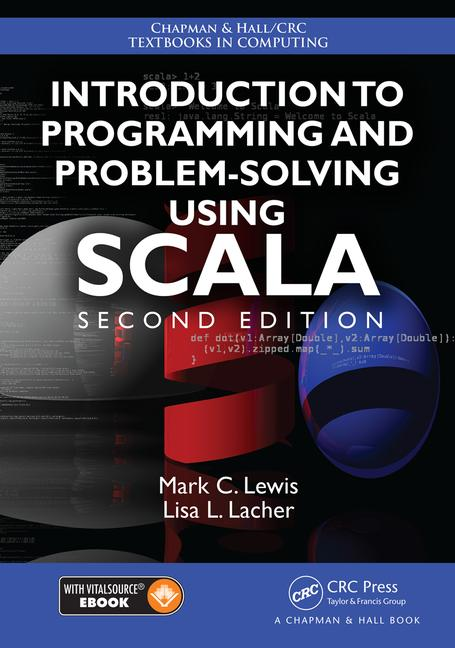
\includegraphics[width=0.33\textwidth]{../img/lewisbook.jpg}\hskip4mm
%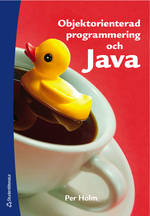
\includegraphics[width=0.33\textwidth]{../img/ankbok.jpg}

\noindent -- för de som \Emph{redan kan OO}:
\vskip0.7mm
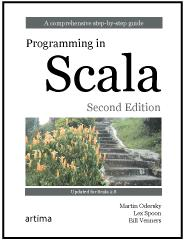
\includegraphics[width=0.45\textwidth]{../img/pinsbook.jpg}\hskip4mm
%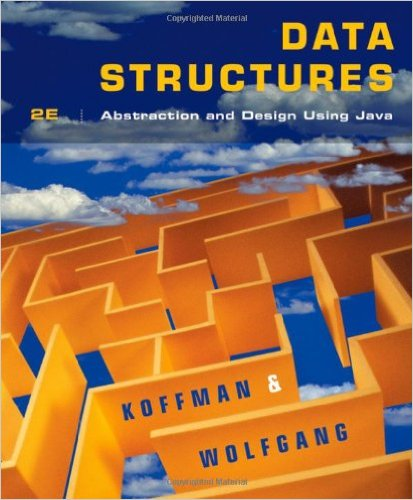
\includegraphics[width=0.47\textwidth]{../img/koffmanbook.jpg}
\end{minipage}
\end{SlideExtra}
\fi

\ifkompendium
\noindent Kompendiet är den huvudsakliga kurslitteraturen och definierar kursinnehållet. Föreläsningar, övningar och laborationer i kompendiet är kursens primära kunskapskällor, tillsammans med de öppna resurser på nätet som kompendiet hänvisar till. Kompendiet är öppen källkod och du välkomnas varmt att bidra!

Om du gärna vill ha en eller flera mer traditionella läroböcker som bredvidläsning rekommenderas följande:
\begin{itemize}[noitemsep, leftmargin=*]
\item För de som aldrig kodat, och vill läsa om kodning från grunden:
\begin{itemize}[nolistsep]
\item ''Introduction to Programming and Problem-Solving Using Scala'' Second Edition (2016), Mark C. Lewis, Lisa Lacher.  %{\href{https://www.crcpress.com/Introduction-to-Programming-and-Problem-Solving-Using-Scala-Second-Edition/Lewis-Lacher/p/book/9781498730952}{www.crcpress.com/Introduction-to-Programming-and-Problem-Solving-Using-Scala-Second-Edition/Lewis-Lacher/p/book/9781498730952}}

\item Lewis \& Lacher täcker stora delar av kursen, men innehåller även en del material som ingår i senare LTH-kurser. Ordningen är ganska annorlunda, men det går bra att läsa boken i en annan ordning än den är skriven.
% \item ''Objektorienterad programmering och Java'', Per Holm, Tredje upplagan (2007). \href{https://www.studentlitteratur.se/#6735}{www.studentlitteratur.se/\#6735}
\end{itemize}
\item För de som redan kodat en hel del i ett objektorienterat språk:
\begin{itemize}[nolistsep, noitemsep]
\item ''Programming in Scala'', Third Edition (2016), Martin Odersky, Lex Spoon, and Bill Venners.  %\\\href{http://www.artima.com/shop/programming_in_scala_3ed}{www.artima.com/shop/programming\_in\_scala\_3ed}
  \item Martin Odersky är upphovspersonen bakom Scala och denna välskrivna bok innehåller en komplett genomgång av Scala-språket med många exempel och tips. ''Third Edition'' täcker Scala version 2.12. Boken riktar sig till de som redan har kunskap om något objektorienterat språk, t.ex. Java. Det finns ett bra index som gör det lätt att anpassa din läsning efter kursens upplägg. Bokens ca 800 sidor innehåller mycket material som är på en mer avancerad nivå än denna kurs, men du kommer att ha nytta av innehållet i kommande kurser.
% \item ''Data Structures: Abstraction and Design Using Java, 3rd Edition'', Elliot B. Koffman, Paul A. T. Wolfgang. \\
% \href{http://eu.wiley.com/WileyCDA/WileyTitle/productCd-1119186528.html}{http://eu.wiley.com/WileyCDA/WileyTitle/productCd-1119186528.html}
\end{itemize}
\end{itemize}
Dessa läroböcker följer inte direkt kursens upplägg vad gäller omfång och progression och du får själv göra den nyttiga hemläxan att koppla  deras innehåll till det vi går igenom i kursens olika moduler.

\else


\begin{SlideExtra}{Beställning av kompendium och snabbreferens}\SlideFontSmall
\begin{itemize}

\item \Emph{Kompendiet} finns i pdf för fri nedladdning enl. CC-BY-SA, men det \Alert{rekommenderas starkt} att du köper den tryckta bokversionen.

\item Det är mycket lättare att ha övningar och labbar \Alert{på papper} \Emph{bredvid skärmen}, när du ska tänka, koda och plugga!

\item \Emph{Snabbreferensen} finns också i pdf men du behöver ha en tryckt version eftersom det är \Alert{enda tillåtna hjälpmedlet} på skriftliga kontrollskrivningen och tentamen.

\item Kompendiet och snabbreferens trycks här i E-huset och säljs av institutionen till \Emph{självkostnadspris}.

\item Pris för kompendium \Alert{beror på hur många som beställer}. Om tillräckligt många köper blir det \Emph{220 kr} inkl. snabbreferens annars \Alert{320} vid köp av enstaka ex i efterhand.

\item Snabbreferens kostar \Alert{40 kr} i enstaka ex men \Emph{ingår i paketet} om du beställer kompendium idag.

\item Kryssa i \Alert{BOK} på listan som snart skickas runt -- tryckning sker sedan enligt din beställning.

\item Du betalar med \Alert{Swish} till \code{123 170 4584} och visar upp betalningsbevis i mobilen för kurssekreterare på \Emph{institutionens expedition}, våning 2.

\end{itemize}
\end{SlideExtra}

\begin{SlideExtra}{Föreläsningsanteckningar}
\begin{itemize}
\item Föreläsningbilder uppdateras under kursens gång.
\item \url{http://cs.lth.se/pgk/foerelaesningar/}
\item Fram till mån kl 13 aktuell vecka är de bilder som ligger ute under pågående uppdatering sedan förra årets version.
\item Latex-koden för alla bilder finns här: \\
\href{https://github.com/lunduniversity/introprog/tree/master/slides}{github.com/lunduniversity/introprog/tree/master/slides}
\item Kom gärna med förslag på innehåll!
\end{itemize}
\end{SlideExtra}
\fi

\ifkompendium\else
\begin{SlideExtra}{Personal \CurrentYear}\SlideFontSmall
\begin{description}
\item [\bfseries Kursansvarig:] Prof. Björn Regnell, bjorn.regnell@cs.lth.se, E:2413
\item [\bfseries Handledare:]\Emph{15st teknologer:}\\
% \Emph{Koordinator}: \\
% %2017:
% Adjunkt Sandra Nilsson
% % 2016: Doktorander MSc. Gustav Cedersjö, Tekn. Lic. Maj Stenmark \\
% \Emph{Teknologer}: (19st) \\
%2019:
\TODO Lista med namn
%2018:
% Emil Wihlander,
% Erik Präntare,
% Henrik Olsson,
% Ivar Henckel,
% Jonatan Nilsson,
% Jos Rosenqvist,
% Klara Broman,
% Linnea Bokelund,
% Ludvig Pärsson,
% Oliver Persson,
% Oskar Berg,
% Oskar Widmark,
% Samer Alkhodary,
% Stefan Jonsson,
% Victor Winberg
%2017:
% Anders	Buhl,
% Erik	Grampp,
% Hampus	Weslien,
% Jakob	Hök,
% Johannes	Tykesson,
% Jonas	Danebjer,
% Jos	Rosenqvist,
% Ludvig	Pärsson,
% Måns	Magnusson,
% Martin	Jakobsson,
% Michael	Young,
% Oskar	Berg,
% Oskar	Widmark,
% Rasmus	Olsson,
% Roland	Holmberg,
% Stefan	Jonsson,
% Tobias	Bladh,
% Victor	Winberg
%2016:
%Anders Buhl,
%Anna Palmqvist Sjövall,
%Anton Andersson,
%Cecilia Lindskog,
%Emil Wihlander,
%Erik Bjäreholt,
%Erik Grampp,
%Filip Stjernström,
%Fredrik Danebjer,
%Henrik Olsson,
%Jakob Hök,
%Jonas Danebjer,
%Måns Magnusson,
%Oscar Sigurdsson,
%Oskar Berg,
%Oskar Widmark,
%Sebastian Hegardt,
%Stefan Jonsson,
%Tom Postema,
%Valthor Halldorsson
\item [\bfseries Kursadmin:]
Ulrika Templing, rum E:2179, Birger Swahn, rum E:2181 \\
Exp.tid: måndag till fredag 9.30-11.30  \\
\url{http://cs.lth.se/kontakt/expedition/} \\
\end{description}
\end{SlideExtra}
\fi


\begin{Slide}{Kursmoment --- varför?}\SlideOnly{\footnotesize}
\begin{itemize}

\item \Emph{Föreläsningar}: skapa översikt, ge struktur, förklara teori, svara på frågor, motivera varför.

\item \Emph{Övningar}: bearbeta teorin steg för steg, \Emph{grundövningar} för alla, \Emph{extraövningar} om du vill/behöver öva mer, \Emph{fördjupningsövningar} om du vill gå djupare; \Alert{förberedelse inför laborationerna}.

\item \Emph{Laborationer}: \Alert{obligatoriska}, sätta samman teorins delar i ett större program; lösningar redovisas för handledare; gk på alla för att få tenta.

\item \Emph{Resurstider}: få hjälp med övningar och laborationsförberedelser av handledare, fråga vad du vill.

\item \Emph{Samarbetsgrupper}: grupplärande genom samarbete, hjälpa varandra.

\item \Emph{Kontrollskrivning}: \Alert{obligatorisk}, diagnostisk, kamraträttad; kan ge samarbetsbonuspoäng till tentan.

\item \Emph{Individuell projektuppgift}: \Alert{obligatorisk}, du visar att du kan skapa ett större program självständigt; redovisas för handledare.

\item \Emph{Tentamen}: \Alert{obligatorisk}, skriftlig, enda hjälpmedel: snabbreferensen.\\   \url{http://cs.lth.se/pgk/quickref}
\end{itemize}
\end{Slide}

\ifkompendium\else
\begin{SlideExtra}{Detta är bara början... }
Exempel på efterföljande kurser som bygger vidare på denna:
\begin{itemize}
\item \Emph{Årskurs 1}
\begin{itemize}
\item Programmeringsteknik -- fördjupningskurs
\item Utvärdering av programvarusystem
\item Diskreta strukturer
\end{itemize}
\item \Alert{Årskurs 2}
\begin{itemize}
\item Objektorienterad modellering och design
\item Programvaruutveckling i grupp
\item Algoritmer, datastrukturer och komplexitet
\item Funktionsprogrammering
\end{itemize}
\end{itemize}
\end{SlideExtra}


\begin{SlideExtra}{Registrering}
\begin{itemize}
\item Fyll i listan \Emph{REGISTRERING EDAA45} som skickas runt.

\item Kryssa i kolumnen \Alert{ÅBEROPAR PLATS} om vill gå kursen\footnote{\scriptsize D1:a som redan gått motsvarande högskolekurs? Uppsök studievägledningen}\footnote{\scriptsize D2:a eller äldre som redan påbörjad EDA016/EDA011/EDA017 el likn.? Övergångsregler: Alla labbar gk: tenta EDA011/017; annars kom och prata på rasten}

\item Kryssa i kolumnen \Emph{BESTÄLLER BOK}

\item Kryssa i kolumnen \Emph{KAN VARA KURSOMBUD} om du kan tänka dig att vara kursombud under kursens gång:
\begin{itemize}
\item Alla LTH-kurser ska utvärderas under kursens gång och efter kursens slut.
\item Till det behövs kursombud -- ungefär \Alert{2 D-are} och \Alert{2 W-are}.
\item Ni kommer att bli kontaktade av studierådet.
\end{itemize}
\end{itemize}
\end{SlideExtra}

\fi


%%%
\ifkompendium\else

\begin{SlideExtra}{Förkunskaper}
\begin{itemize}
\item Förkunskaper $\neq$ Förmåga
\item Varken kompetens eller personliga egenskaper är statiska
\item ''Programmeringskompetens'' är inte \textit{en} enda enkel förmåga utan en komplex sammansättning av flera olika förmågor som \Emph{utvecklas} genom hela livet
\item Ett innovativt utvecklar\Alert{team} behöver många olika kompetenser för att vara framgångsrikt
\end{itemize}
\end{SlideExtra}
\fi

\ifkompendium\else

%%%
\begin{SlideExtra}{Förkunskapsenkät}
\begin{itemize}
\item Om du inte redan gjort det fyll i förkunskapsenkäten \Alert{snarast}:
\url{http://cs.lth.se/pgk/introsurvey}
\item Dina svar behandlas internt och all redovisad statistik anonymiseras.
\item Enkäten ligger till grund för randomiserad gruppindelning i samarbetsgrupper, så att det blir en spridning av förkunskaper inom gruppen.
\item Gruppindelning publiceras här: \\ \url{http://cs.lth.se/pgk/grupp}
\item Ditt gruppnummer (t.ex. D1.7b) styr vilken schema grupp du tillhör (t.ex. D1.7), se \url{http://cs.lth.se/pgk/schema/} Schema TimeEdit
\end{itemize}
\end{SlideExtra}

\begin{SlideExtra}{Samarbetgrupper}\footnotesize
\begin{itemize}
\item Ni delas in i \Emph{samarbetsgrupper} om ca 5 personer baserat på förkunskapsenkäten, så att olika förkunskapsnivåer sammanförs
\item En av laborationerna (\code{snake}) i lp2 är en mer omfattande \Emph{grupplabb} och kommer att göras i din samarbetsgrupp. \\ \vspace{1em}
\item Kontrollskrivningen i halvtid kan ge \Emph{samarbetsbonus} (max 5p) som adderas till ordinarie tentans poäng (max 100p) med medelvärdet av gruppmedlemmarnas individuella kontrollskrivningspoäng
\scriptsize \parbox{7cm}{Bonus $b$ för varje person i en grupp med $n$ medlemmar med $p_i$ poäng vardera på kontrollskrivningen:}
 \hspace{5mm} $\displaystyle b = \sum\limits_{i=1}^n \frac{p_i}{n}$
\end{itemize}
\end{SlideExtra}



%%%
\begin{SlideExtra}{Varför studera i samarbetsgrupper?}

Huvudsyfte: \Emph{Bra lärande!}

\begin{itemize}
\item Pedagogisk forskning stödjer tesen att lärandet blir mer djupinriktat om det sker i utbyte med andra
\item Ett studiesammanhang med \Alert{höga ambitioner} och \Alert{respektfull gemenskap} gör att vi \Emph{når mycket längre}
\item Varför ska du som redan kan mycket aktivt dela med dig av dina kunskaper?
\begin{itemize}
\item Förstå bättre själv genom att förklara för andra
\item Träna din pedagogiska förmåga
\item Förbered dig för ditt kommande yrkesliv som mjukvaruutvecklare
\end{itemize}
\end{itemize}
\end{SlideExtra}

%%%

\begin{SlideExtra}{Samarbetskontrakt}
Gör ett skriftligt \href{https://github.com/lunduniversity/introprog/tree/master/study-groups}{\Emph{samarbetskontrakt}} med dessa och ev. andra punkter som ni också tycker bör ingå:
\begin{enumerate}
\item Återkommande mötestider per vecka
\item Kom i tid till gruppmöten
\item Var väl förberedd genom självstudier inför gruppmöten
\item Hjälp varandra att förstå, men ta inte över och lös allt
\item Ha ett respektfullt bemötande även om ni har olika åsikter
\item Inkludera alla i gemenskapen
\end{enumerate}

Diskutera hur ni ska uppfylla dessa innan alla skriver på. \\ Ta med samarbetskontraktet och visa för handledare på labb 1.

\vskip1em

\Alert{Om arbetet i samarbetsgruppen inte fungerar ska ni mejla kursansvarig och boka mötestid!}
\end{SlideExtra}

\begin{SlideExtra}{Bestraffa inte frågor!}
\begin{itemize}
\item Det finns bättre och sämre frågor vad gäller hur mycket man kan lära sig av svaret, men \Emph{all undran är en chans} att i dialog utbyta erfarenheter och lärande.
\item Den som frågar \Emph{vill veta} och berättar genom frågan något om nuvarande kunskapsläge.
\item Den som svarar får chansen att \Emph{reflektera} över vad som kan vara svårt och olika vägar till djupare förståelse.
\item I en hälsosam lärandemiljö är det \Emph{helt tryggt} att visa att man \Alert{ännu inte förstår}, att man gjort ''fel'', att man har mer att lära, etc.
\item Det är viktigt att \Emph{våga försöka} även om det blir \Alert{''fel''}:\\ \Alert{det är ju då man lär sig!}
\end{itemize}
\end{SlideExtra}

%%%
\begin{SlideExtra}{Plagiatregler}
\begin{itemize}
\item Läs dessa regler noga och diskutera i samarbetsgrupperna:

\begin{itemize}
\footnotesize
\item \url{http://cs.lth.se/utbildning/samarbete-eller-fusk/}
\item \href{http://cs.lth.se/utbildning/foereskrifter-angaaende-obligatoriska-moment/}{Föreskrifter angående obligatoriska moment}
\end{itemize}
\item Ni ska lära er genom \Emph{eget arbete} och genom  \Emph{bra samarbete}.
\item Samarbete gör att man lär sig bättre, men man lär sig \Alert{inte} av att bara kopiera andras lösningar.
\item \Alert{Plagiering är förbjuden} och kan medföra \Alert{disciplinärende och avstängning}.
\item Du får \Alert{INTE} lägga ut laborationslösningar öppet på \Emph{\code{github}} eller på annan plats där någon annan kan komma åt dem!
\end{itemize}

\end{SlideExtra}

\fi %%%%%%%%%%%%%%%%%%%%%%%%%%%%%%%%

%%%
\begin{Slide}{En typisk kursvecka}
\begin{enumerate}
\item Gå på \Emph{föreläsningar} på \Alert{måndag--tisdag}
\item \Alert{Jobba} \Emph{individuellt} med teori, övningar, labbförberedelser på  \Alert{måndag--torsdag}
\item \Alert{Träffas} i \Emph{samarbetsgruppen} och hjälp varandra att förstå mer och fördjupa lärandet, förslagsvis på återkommande tider varje vecka då alla i gruppen kan
\item Kom till \Emph{resurstiderna} och få hjälp och tips av handledare och kurskamrater på \Alert{onsdag--torsdag}
\item Genomför den obligatoriska \Emph{laborationen} på \Alert{fredag}
\end{enumerate}
Se detaljerna och undantagen i schemat: \href{http://cs.lth.se/pgk/schema}{cs.lth.se/pgk/schema}
\end{Slide}

\ifkompendium\else  %%%%%%%%%%%%%%%%%%%%%%%%%
%%%
\begin{SlideExtra}{Övningar}\SlideFontSmall
\begin{itemize}
  \item \Alert{Programmering lär man sig bäst genom att programmera...}

\item Genom övningarna bearbetar du teorins olika delar via egna \Emph{undersökningar} med \Alert{Scala REPL} som viktigaste verktyg.

\item Fokusera på att \Emph{förstå} vad som händer när du kör din kod. Om du bara rusar vidare utan reflektion lär du dig inte alls lika bra.

\item Till de flesta övningar finns facit. Titta inte på facit förrän du själv gjort ett försök. Det finns ofta många olika sätt att åstadkomma samma sak, och din lösningsvariant kan vara lika bra som den i facit -- använd REPL för att verifiera att din lösning fungerar. Diskutera med handledare om du är osäker på vad som är ok.

\item Skapa en miljö för \Emph{koncentration} och lärande \Emph{på djupet}. Stäng telefon, be kompisar i datorsalen att inte prata för högt, etc.
\end{itemize}
\end{SlideExtra}

\begin{SlideExtra}{Laborationer}\SlideFontSmall
\begin{itemize}
\item På laborationerna \Emph{sammanför} du veckans koncept till en \Emph{helhet} i ett större program och kollar att du \Alert{kan grunderna} inför kommande veckor.
\item Labbarna är \Emph{individuella} (utom en) och \Emph{obligatoriska}.

\item Gör \Emph{övningarna} och \Emph{labbförberedelserna} noga \Alert{innan} själva labben -- detta är ofta helt nödvändigt för att du ska hinna klart. Dina labbförberedelser kontrolleras av handledare under labben.

\item Är du \Emph{sjuk?} Anmäl det \Alert{före} labben till \url{bjorn.regnell@cs.lth.se}, \\ få hjälp på resurstid och redovisa på resurstid (eller labbtid, när handledaren har tid över)

\item Hinner du inte med hela labben? Se till att handledaren noterar \Alert{''kompletteras''}, och fortsätt på resurstid och ev. uppsamlingstider.

\item Läs noga kapitel noll ''\Alert{Anvisningar}'' i kompendiet!

\item Laborationstiderna är gruppindelade enligt \href{http://cs.lth.se/pgk/schema/}{schemat}. Du ska gå till den tid och den sal som motsvarar din grupp som visas i \href{http://cs.lth.se/pgk/schema/timeedit/}{TimeEdit}.\\
\Emph{Gruppindelning} blir ''klar'' senast i morgon tisdag kl 13.
\\Nya versioner släpps här: \url{http://cs.lth.se/pgk/grupp}
\\OBS! Rensa cachen (Ctrl+F5) och kolla versionsnummer.
\end{itemize}
\end{SlideExtra}

%%%
\begin{SlideExtra}{Resurstider}\SlideFontTiny
\begin{itemize}
\item På resurstiderna får du \Emph{hjälp}  med \Alert{övningar} och labb\Alert{förberedelser}.

\item Kom till minst en resurstid per vecka, se \href{http://cs.lth.se/pgk/schema/timeedit}{Schema i TimeEdit}.

%\item Handledare gör ibland \Emph{genomgångar} för alla under resurstiderna. Tipsa om handledare om vad du finner svårt!
\item Du får i mån av plats gå på flera resurstider per vecka. Om det blir fullt i ett rum prioriteras schemagrupper:
\end{itemize}
\begin{table}[]
\centering\SlideFontTiny
\begin{tabular}{lllll}
\Emph{Tid Lp1} & \Emph{Sal} & \Alert{Grupper med prio} \\
\hline
Ons 10-12 v1-7 & Falk &  D1.01 \\
Ons 10-12 v1-7 & Val  &  D1.02 \\
Ons 13-15 v1-7 & Falk &  D1.11 \\
Ons 13-15 v1-7 & Val  &  D1.12 \\
Ons 13-15 v1-7 & Varg &  D1.13 \\
Ons 15-17 v1-7 & Falk &  D1.07 \\
Ons 15-17 v1-7 & Val  &  D1.08 \\ \hline
Tor 10-12 v1-7 & Falk &  D1.00 \\
Tor 10-12 v1-7 & Val  &  D1.10 \\
Tor 13-15 v1-7 & Falk &  D1.03 \\
Tor 13-15 v1-7 & Val  &  D1.04 \\
Tor 15-17 v1-7 & Falk &  D1.05 \\
Tor 15-17 v1-7 & Val  &  D1.06 \\
\end{tabular}
\end{table}
W-are tilldelas D-schemagrupp enl. samarbetsgruppindelningen.
\end{SlideExtra}

\fi


\ifkompendium\else
\begin{SlideExtra}{På Rasten...}
\begin{itemize}
  \item Uppropslista fastställs
  \item Ev. önskemål ang. gruppindelning pga speciella skäl
  \item Kompendietryckbeställning sista chansen
  \item Bläddra i bredvidläsning
  \item ...
\end{itemize}
\end{SlideExtra}
\fi

%!TEX encoding = UTF-8 Unicode
%!TEX root = ../lect-w01.tex

%%%%%%%%%%%%%%%%%%%%%%%%%%%%%%%%%%%%%%

\Subsection{Att lära denna läsvecka \texttt{w01}}

\ifkompendium\else  %%%%%%%%%%%%%%%%%%%%%%%%%%%%%%%%%%%%%%%%%%%%%%%%%
\begin{SlideExtra}{Att lära denna läsvecka \texttt{w01}}
%!TEX encoding = UTF-8 Unicode

    Modul \Emph{Introduktion}: Övn \Alert{\texttt{expressions}} $\rightarrow$ Labb \Alert{\texttt{kojo}}
    \begin{multicols}{3}\SlideFontTiny
    $\square$ sekvens \\
$\square$ alternativ \\
$\square$ repetition \\
$\square$ abstraktion \\
$\square$ editera \\
$\square$ kompilera \\
$\square$ exekvera \\
$\square$ datorns delar \\
$\square$ virtuell maskin \\
$\square$ litteral \\
$\square$ värde \\
$\square$ uttryck \\
$\square$ identifierare \\
$\square$ variabel \\
$\square$ typ \\
$\square$ tilldelning \\
$\square$ namn \\
$\square$ val \\
$\square$ var \\
$\square$ def \\
$\square$ definera och anropa funktion \\
$\square$ funktionshuvud \\
$\square$ funktionskropp \\
$\square$ procedur \\
$\square$ inbyggda grundtyper \\
$\square$ Int \\
$\square$ Long \\
$\square$ Short \\
$\square$ Double \\
$\square$ Float \\
$\square$ Byte \\
$\square$ Char \\
$\square$ String \\
$\square$ println \\
$\square$ typen Unit \\
$\square$ enhetsvärdet () \\
$\square$ stränginterpolatorn s \\
$\square$ if \\
$\square$ else \\
$\square$ true \\
$\square$ false \\
$\square$ MinValue \\
$\square$ MaxValue \\
$\square$ aritmetik \\
$\square$ slumptal \\
$\square$ math.random \\
$\square$ logiska uttryck \\
$\square$ de Morgans lagar \\
$\square$ while-sats \\
$\square$ for-sats \\
    \end{multicols}
    
\end{SlideExtra}
\fi

\Subsection{Om programmering}

\ifkompendium\else  %%%%%%%%%%%%%%%%%%%%%%%%%%%%%%%%%%%%%%%%%%%%%%%%%

\begin{SlideExtra}{Att skapa koden som styr världen}
\begin{multicols}{2}\footnotesize
I stort sett \Alert{alla} delar av samhället är beroende av programkod:
\begin{itemize}\scriptsize
\item kommunikation
\item transport
\item byggsektorn
\item statsförvaltning
\item finanssektorn
\item media \& underhållning
\item sjukvård
\item övervakning
\item integritet
\item upphovsrätt
\item miljö \& energi
\item sociala relationer
\item utbildning
\item ...
\end{itemize}
\columnbreak %---------
Hur blir ditt framtida yrkesliv som systemutvecklare?
\begin{itemize}
\item  Det är sedan lång tid en \Alert{skriande brist} på utvecklare och det blir bara värre... \\
\href{https://cio.idg.se/2.1782/1.710012/kompetenslarm-jobb-om-fem-ar?queryText=kompetensbrist}{CIO 2018-11-09} %\\
%\href{http://computersweden.idg.se/2.2683/1.663879/oppen-kallkod-brist-kompetens}{CS 2016-08-23} 

\item Störst brist är det på \Emph{kvinnliga} utvecklare: \\
\href{https://www.svt.se/nyheter/inrikes/stor-brist-pa-programmerare-kvinnor-lockas-till-yrket}{SVT 2016-12-03}

\item Global kompetensmarknad \\
  \href{https://cio.idg.se/2.1782/1.648294/hitta-it-kompetens/sida/2/global-rekrytering-aktivt-hr-arbete}{CIO 2016-02-01}\\
  \href{http://computersweden.idg.se/2.2683/1.630901/det-finns-programmerare-och-sa-finns-det-programmerare}{CS 2015-06-14} \\
  \href{http://computersweden.idg.se/2.2683/1.662186/25-miljoner-utvecklare?queryText=miljoner\%20utvecklare}{CS 2016-07-14 }
\end{itemize}
\end{multicols}

\end{SlideExtra}

\begin{SlideExtra}{Utveckling av mjukvara i praktiken}
\begin{itemize}
\item \Emph{Inte bara kodning:} kravbeslut, releaseplanering, design, test, versionshantering, kontinuerlig integration, driftsättning, återkoppling från dagens användare, ekonomi \& investering, gissa om morgondagens användare, ...
\item \Emph{Teamwork:} Inte ensamma hjältar utan autonoma team i decentraliserade organisationer med innovationsuppdrag
\item \Emph{Snabbhet:} Att koda innebär att hela tiden uppfinna nya ''byggstenar'' som ökar organisationens förmåga att snabbt skapa värde med hjälp av mjukvara. \Alert{Öppen källkod}. Skapa kraftfulla API:er.
\item \Emph{Livslångt lärande:} Lär nytt och dela med dig hela tiden. Exempel på pedagogisk utmaning: hjälp andra förstå och använda ditt API $\implies$ \Alert{Samarbetskultur}
\end{itemize}
\end{SlideExtra}


\fi %%%%%%%%%%%%%%%%%%%%%%%%%%%%%%%%%%%%%%%%%%%%%%%%%%%%


% \ifkompendium\else
% \SlideImg{Programming unplugged: Två frivilliga?}{../img/unplugged}
% \SlideImg{Editera och exekvera ett program}{../img/kojo}
% \fi

%%%

\ifkompendium\else
\SlideImg{Vad är en dator?}{../img/eniac}
\fi

\begin{Slide}{Hur fungerar en dator?}
\begin{tikzpicture}[node distance=2.0cm]
\node (input)  [startstop]               {Indata-enhet};
\node (cpu)    [process, below of=input] {CPU};
\node (output) [startstop,below of=cpu]  {Utdata-enhet};

\node (mem) [right of=cpu, xshift=0.4\textwidth, draw = black, thick] {
\begin{minipage}{0.5\textwidth}\centering
\textbf{Minne} med minnesceller
\vspace{1em}

\begin{tabular}{|l | l|}
address & innehåll \\ \hline
0   & 42 \\ \hline
1   & 13 \\ \hline
2   & 18 \\ \hline
3   & 21 \\ \hline
4   & 55 \\ \hline
5   & 64 \\ \hline
6   & 48 \\ \hline
... & ...
\end{tabular}
\end{minipage}
};

\draw [arrow] (input) -- (cpu);
\draw [arrow] (cpu) -- (output);
\draw [arrow] (cpu) -- (mem);
\draw [arrow] (mem) -- (cpu);

\end{tikzpicture}

{\hfill
\begin{minipage}{0.65\textwidth}\vspace{1em}
Minnet innehåller endast \Alert{heltal} som \newline representerar \Emph{data} \Alert{och} \Emph{instruktioner}.
\end{minipage}
}
\end{Slide}

\begin{Slide}{Vad är programmering?}
\begin{itemize}
\item Programmering innebär att ge instruktioner till en maskin.
\item Ett \Emph{programmeringsspråk} används av människor för att skriva \Emph{källkod} som kan översättas av en \Emph{kompilator} till \Emph{maskinspråk} som i sin tur \Emph{exekveras} av en dator.
\end{itemize}


\begin{minipage}{.8\textwidth}
\begin{itemize}
\item Ada Lovelace publicerade det första programmet redan på 1800-talet ämnat för en kugghjulsdator.
\end{itemize}
\end{minipage}%
\begin{minipage}{.2\textwidth}
\centering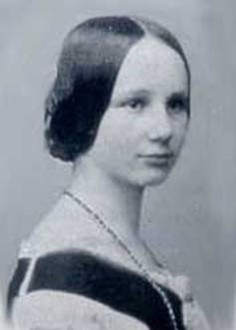
\includegraphics[width=0.6\columnwidth]{../img/ada}
\end{minipage}%
\begin{itemize}
\item \href{https://sv.wikipedia.org/wiki/Programmering}{sv.wikipedia.org/wiki/Programmering}
\item \href{https://en.wikipedia.org/wiki/Computer\_programming}{en.wikipedia.org/wiki/Computer\_programming}
\item Ha picknick i \href{http://kartor.lund.se/wiki/lundanamn/index.php/Ada_Lovelace-parken}{Ada Lovelace-parken} på Brunnshög!
\end{itemize}
\end{Slide}


\begin{Slide}{Vad är en kompilator?}
\begin{minipage}{.35\textwidth}
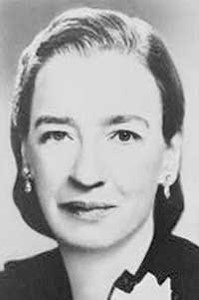
\includegraphics[width=0.6\textwidth]{../img/grace}
\end{minipage}%
\begin{minipage}{.67\textwidth}
%https://www.sharelatex.com/blog/2013/08/29/tikz-series-pt3.html
\begin{tikzpicture}[node distance=1.4cm,scale=0.8]
  \node (input) [startstop] {Källkod};
  \node(inptext) [right of=input, text width=2cm, scale=0.8,xshift=1.5cm]{För\\människor};
  \node (compile) [process, below of=input] {Kompilator};
  \node (output) [startstop, below of=compile] {Maskinkod};
  \node(outtext) [right of=output, text width=2cm, scale=0.8,xshift=1.5cm]{För\\maskiner};
  \draw [arrow] (input) -- (compile);
  \draw [arrow] (compile) -- (output);
  \end{tikzpicture}%

\vspace{1em}\noindent Grace Hopper uppfann kompilatorn 1952. \\ \href{https://en.wikipedia.org/wiki/Grace\_Hopper}{\SlideFontTiny en.wikipedia.org/wiki/Grace\_Hopper}
\end{minipage}%
\end{Slide}


\begin{Slide}{Virtuell maskin (VM) == abstrakt hårdvara}
\begin{multicols}{2}
\begin{itemize}
\item En VM är en ''dator'' implementerad i mjukvara som kan tolka en generell ''maskinkod'' som \Emph{översätts under körning} till den \Alert{verkliga} maskinens specifika maskinkod.

\item Med en VM blir källkoden \Emph{plattformsoberoende} och fungerar på många olika maskiner.

\item Exempel JVM: \\ \Emph{Java Virtual Machine}


\end{itemize}

\columnbreak %---------

%https://www.sharelatex.com/blog/2013/08/29/tikz-series-pt3.html
\begin{tikzpicture}[node distance=1.4cm]
\node (input) [startstop] {Källkod};
\node (compile) [process, below of=input] {Kompilator};
\node (output) [startstop, below of=compile] {Generell ''maskinkod''};
\node (interp) [process, below of=output] {VM interpreterar};
\node (output2) [startstop, below of=interp] {Specifik maskinkod};
\draw [arrow] (input) -- (compile);
\draw [arrow] (compile) -- (output);
\draw [arrow] (output) -- (interp);
\draw [arrow] (interp) -- (output2);
\end{tikzpicture}
\end{multicols}
\end{Slide}

\begin{Slide}{Vad består ett program av?}
\begin{itemize}
\item Text som följer entydiga språkregler (grammatik):
\begin{itemize}
\item \Emph{Syntax}: textens konkreta utseende
\item \Emph{Semantik}: textens betydelse (vad maskinen gör/beräknar)
\end{itemize}
\item \Emph{Nyckelord}: ord med speciell betydelse, t.ex. \code{if}, \code{else}
\item \Emph{Deklarationer}: definitioner av nya ord: \code{def gurka = 42}
\item \Emph{Satser} är instruktioner som \Alert{gör} något: \code{print("hej")}
\item \Emph{Uttryck} är instruktioner som beräknar ett \Alert{resultat}: \code{1 + 1}
\item \Emph{Data} är information som behandlas: t.ex. heltalet \code{42}
\item Instruktioner ordnas i kodstrukturer: \Alert{SARA}
\begin{itemize}
  \item \Emph{Sekvens}: ordningen spelar roll för vad som händer
  \item \Emph{Alternativ}: olika resultat beroende på uttrycks värde
  \item \Emph{Repetition}: instruktioner upprepas många gånger
  \item \Emph{Abstraktion}: nya byggblock skapas för att återanvändas
\end{itemize}
\end{itemize}
\end{Slide}

\begin{Slide}{Exempel på programmeringsspråk}
Det finns massor med olika språk och det kommer ständigt nya.
\vspace{1em}
\begin{multicols}{2}
Exempel:
\begin{itemize}
\item Java
\item C
\item C++
\item C\#
\item Python
\item JavaScript
\item Scala
\end{itemize}

\columnbreak %---------

Topplistor:
\begin{itemize}
\item \href{https://redmonk.com/sogrady/2020/07/27/language-rankings-6-20/}{Redmonk language rankings}   
%\item \href{https://redmonk.com/sogrady/2019/07/18/language-rankings-6-19/}{Redmonk language rankings}   
%\item \href{https://redmonk.com/sogrady/2018/08/10/language-rankings-6-18/}{Redmonk language rankings}   
\item \href{http://pypl.github.io/PYPL.html}{PYPL Index}
\item \href{http://www.tiobe.com/index.php/content/paperinfo/tpci/index.html}{TIOBE Index}
\end{itemize}
% \vspace{1em}
% 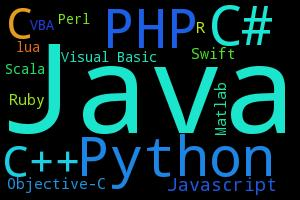
\includegraphics[width=0.8\columnwidth]{../img/pypl}\\\SlideFontSmall{[PYPL (2016)]}
\end{multicols}

\end{Slide}

\ifkompendium\else
\begin{SlideExtra}{Redmonk Language Rankings: Github, Stackoverflow}
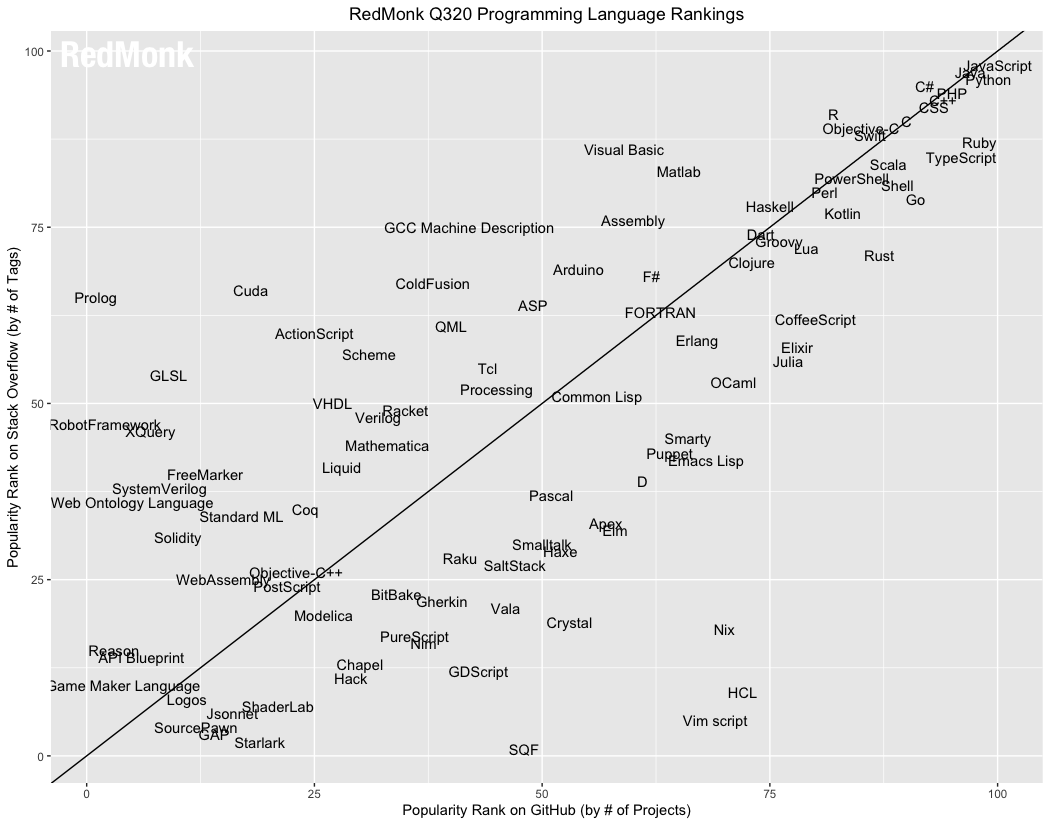
\includegraphics[width=0.95\columnwidth]{../img/redmonk-Q320}
\end{SlideExtra}
\begin{SlideExtra}{Några språks utveckling över tid enl. PYPL}
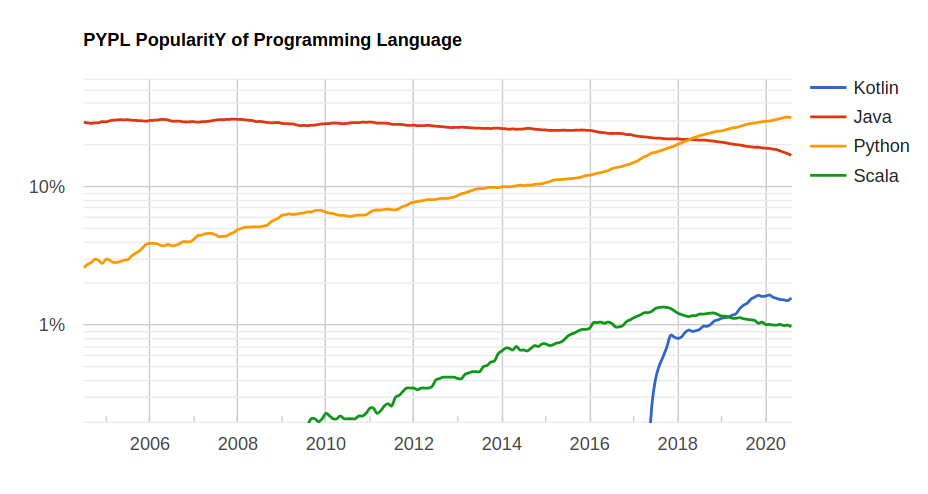
\includegraphics[width=0.95\columnwidth]{../img/pypl-06-20}
\end{SlideExtra}

\fi

\begin{Slide}{Olika programmeringsparadigm}
\begin{itemize}
\item Det finns många olika \href{https://en.wikipedia.org/wiki/Programming_paradigm}{programmeringsparadigm} (sätt att programmera på), till exempel:
\begin{itemize}\SlideFontSmall
\item \Emph{imperativ programmering:} programmet är uppbyggt av sekvenser av olika satser som påverkar systemets tillstånd
\item \Emph{objektorienterad programmering:} en sorts imperativ programmering där programmet består av objekt som sammanför data och operationer på dessa data
\item \Emph{funktionsprogrammering:} programmet är uppbyggt av samverkande (matematiska) funktioner som undviker föränderlig data och tillståndsändringar
\item \Emph{deklarativ programmering, logikprogrammering:} programmet är uppbyggt av logiska uttryck som beskriver olika fakta eller villkor och exekveringen utgörs av en bevisprocedur som söker efter värden som uppfyller fakta och villkor
\end{itemize}
\end{itemize}
\end{Slide}


\begin{Slide}{Hello world}

Scala-skript:
\begin{REPLnonum}
scala> println("Hello World!")
Hello World!
\end{REPLnonum}

Scala-applikation:
\begin{Code}
object Hello {
  def main(args: Array[String]): Unit = println("Hello world!")
}
\end{Code}

Java-applikation:
\begin{Code}[language=Java]
public class Hello {
    public static void main(String[] args) {
        System.out.println("Hello world!");
    }
}
\end{Code}

\end{Slide}

\begin{Slide}{Utvecklingscykeln}
editera; kompilera; hitta fel och förbättringar; editera; kompilera; hitta fel och förbättringar; editera; kompilera; hitta fel och förbättringar; editera; kompilera; hitta fel och förbättringar; editera; kompilera; hitta fel och förbättringar; editera; kompilera; hitta fel och förbättringar; ...

\begin{Code}
upprepa(1000){
  editera
  kompilera
  testa
}
\end{Code}
\end{Slide}

\begin{Slide}{Utvecklingsverktyg}
\begin{itemize}
\item Din verktygskunskap är mycket viktig för din produktivitet.
\item Lär dig kortkommandon för vanliga handgrep.
\item Verktyg vi använder i kursen:
\begin{itemize}
\item Scala \Emph{REPL}: från övn 1
\item \Emph{Texteditor} för kod, t.ex VS \code{code}: från övn 2
\item Kompilera med \Emph{\code{scalac}} och \Emph{\code{javac}}: från övn 2
\item Integrerad utvecklingsmiljö (IDE)
\begin{itemize}
\item \Emph{Kojo}: från lab 1
\item \Emph{IntelliJ IDEA} (alt. ScalaIDE/Eclipse): från läsperiod 2
\end{itemize}
\item \Emph{jar} för att packa ihop och distribuera klassfiler
\item \Emph{javadoc} och \Emph{scaladoc} för dokumentation av kodbibliotek
\end{itemize}
\item Andra verktyg som är bra att lära sig:
\begin{itemize}
\item git för versionshantering
\item GitHub för kodlagring -- men \Alert{inte} av lösningar till labbar!
\end{itemize}
\end{itemize}
\end{Slide}





\Subsection{De enklaste beståndsdelarna: litteraler, uttryck, variabler}


\begin{Slide}{Litteraler}
\begin{itemize}
\item En literal representerar ett fixt \Emph{värde} i koden och används för att skapa \Alert{data} som programmet ska bearbeta.
\item Exempel: \\
\begin{tabular}{l l}
\code|42| & heltalslitteral\\
\code|42.0| & decimaltalslitteral\\
\code|'!'| & teckenlitteral, omgärdas med 'enkelfnuttar' \\
\code|"hej"| & stränglitteral, omgärdas med ''dubbelfnuttar'' \\
\code|true| & litteral för sanningsvärdet ''sant''\\
\end{tabular}
\item Literaler har en \Emph{typ} som avgör vad man kan göra med dem.
\end{itemize}
\end{Slide}

\begin{Slide}{Exempel på inbyggda datatyper i Scala}\SlideFontSmall
\begin{itemize}
\item Alla värden, uttryck och variabler har en \href{https://sv.wikipedia.org/wiki/Datatyp}{\Emph{datatyp}}, t.ex.:
\begin{itemize}\footnotesize
\item \code{Int} för heltal
\item \code{Long} för \textit{extra} stora heltal (tar mer minne)
\item \code{Double} för decimaltal, så kallade flyttal med flytande decimalpunkt
\item \code{String} för strängar
\end{itemize}

\item Kompilatorn håller reda på att uttryck kombineras på ett \Emph{typsäkert} sätt. Annars blir det \Alert{kompileringsfel}.

\item Scala och Java är s.k. \href{https://sv.wikipedia.org/wiki/Typsystem}{\Emph{statiskt typade}} språk, vilket innebär att kontroll av typinformation sker vid kompilering \Eng{compile time}\footnote{Andra språk, t.ex. Python och Javascript är \Emph{dynamiskt typade} och där skjuts typkontrollen upp till körningsdags \Eng{run time} \\ Vilka är för- och nackdelarna med statisk vs. dynamisk typning?}.

\item Scala-kompilatorn gör \href{https://en.wikipedia.org/wiki/Type_inference}{\Emph{typhärledning}}: man \Alert{slipper skriva typerna} om kompilatorn kan lista ut dem med hjälp av typerna hos deluttrycken.

\end{itemize}
\end{Slide}


\begin{Slide}{Grundtyper i Scala}\SlideFontSmall
Dessa \Emph{grundtyper} \Eng{basic types} finns inbyggda i Scala:

\begin{table}[H]
\renewcommand{\arraystretch}{1.4}
\begin{tabular}{p{0.24\textwidth}|p{0.21\textwidth}|l}
\textit{Svenskt namn} & \textit{Engelskt namn} & \Emph{Grundtyper} \\ \hline
heltalstyp & integral type & \texttt{Byte}, \texttt{Short}, \texttt{Int}, \texttt{Long}, \texttt{Char} \\
flyttalstyp  &  floating point \newline number types & \texttt{Float}, \texttt{Double} \\
numeriska typer & numeric types & heltalstyper och flyttalstyper \\
strängtyp \newline (teckensekvens) & string type & \texttt{String}  \\
sanningsvärdestyp  \newline (boolesk typ)& truth value type & \texttt{Boolean} \\
\end{tabular}
\end{table}

\end{Slide}

\begin{Slide}{Grundtypernas implementation i JVM}\SlideFontSmall
\begin{table}[H]
\renewcommand{\arraystretch}{1.4}
\begin{tabular}{l|l|l|l}
\Alert{Grundtyp} i &  Antal                &      Omfång&\Alert{primitiv typ} i\\
 \Emph{Scala} & bitar & minsta/största värde &\Emph{Java} \& \Emph{JVM}\\ \hline
\texttt{Byte}   &  8  & $-2^7$ ... $2^7-1$   & \texttt{byte} \\
\texttt{Short}  &  16 & $-2^{15}$ ... $2^{15}-1$ & \texttt{short} \\
\texttt{Char}   &  16 & $0$ ... $2^{16}-1$ & \texttt{char} \\
\texttt{Int}    &  32 & $-2^{31}$ ... $2^{31}-1$ & \texttt{int} \\
\texttt{Long}   &  64 & $-2^{63}$ ... $2^{63}-1$ & \texttt{long} \\
\texttt{Float}  &  32 & ± $3.4028235 \cdot 10^{38}$  & \texttt{float} \\
\texttt{Double} &  64 & ± $1.7976931348623157 \cdot 10^{308}$ & \texttt{double} \\
\end{tabular}
\end{table}

Grundtypen \texttt{String} lagras som en \emph{sekvens} av 16-bitars tecken av typen \texttt{Char} och kan vara av godtycklig längd (tills minnet tar slut).

\end{Slide}


\begin{Slide}{Uttryck}
\begin{itemize}
\item Ett \Emph{uttryck} består av en eller flera delar som efter \Emph{evaluering} ger ett \Alert{resultat}.
\item Delar i ett uttryck kan t.ex. vara: \\ literaler (42), operatorer (+), funktioner (sin), ...
\item Exempel:
\begin{itemize}
\item Ett enkelt uttryck: \\ \code{42.0}
\item Sammansatta uttryck: \\
\code{40 + 2} \\
\code{(20 + 1) * 2} \\
\code{sin(0.5 * Pi)} \\
\code{"hej" + " på " + "dej"}
\end{itemize}

\item När programmet tolkas sker \Emph{evaluering} av uttrycket, vilket ger ett resultat i form av ett \Emph{värde} som har en \Emph{typ}.
\end{itemize}
\end{Slide}


\begin{Slide}{Variabler}\SlideFontSmall
\begin{itemize}
\item En \Emph{variabel} kan tilldelas värdet av ett enkelt eller sammansatt uttryck.
\item En variabel har ett \Emph{variabelnamn}, vars utformning följer språkets regler för s.k. \Emph{identifierare}.
\item En ny variabel införs i en \Emph{variabeldeklaration} och då den kan ges ett värde, \Emph{initialiseras}. Namnet användas som \Emph{referens} till värdet.
\item Exempel på variabeldeklarationer i Scala, notera \Emph{nyckelordet} \code{val}:
\begin{Code}
val a = 0.5 * Pi
val length = 42 * sin(a)
val exclamationMarks = "!!!"
val greetingSwedish = "Hej på dej" + exclamationMarks
\end{Code}

\item Vid exekveringen av programmet lagras variablernas värden i minnet och deras respektive värde hämtas ur minnet när de \Emph{refereras}.

\item Variabler som deklareras med \code{val} kan endast tilldelas ett värde \Alert{en enda gång}, vid den initialisering som sker vid deklarationen.
\end{itemize}

\end{Slide}


\begin{Slide}{Regler för identifierare}
\begin{itemize}
\item \Emph{Enkel} identifierare: t.ex. \code{gurka2tomat}
\begin{itemize}
\item Börja med bokstav
\item ...följt av bokstäver eller siffror
\item Kan även innehålla understreck
\end{itemize}

\item \Emph{Operator}-identifierare, t.ex. \code{+:}
\begin{itemize}
\item Börjar med ett \Emph{operatortecken}, t.ex. \code{+ - * / : ? ~ #}
\item Kan följas av fler operatortecken
\end{itemize}


\item En identifierare får \Alert{inte} vara ett \Emph{reserverat ord}, se \href{http://cs.lth.se/pgk/quickref}{snabbreferensen} för alla reserverade ord i Scala \& Java.

\item \Emph{Bokstavlig} identifierare: \code{`kan innehålla allt`}
\begin{itemize}
\item Börjar och slutar med \Emph{backticks}  \code{` `}
\item Kan innehålla vad som helst (utom backticks)
\item Kan användas för att undvika krockar med reserverade ord: \texttt{\code{`}val\code{`}}
\end{itemize}

\end{itemize}
\end{Slide}



%\begin{Slide}{Regler för identifierare i Java}\footnotesize
%När kompilatorn ''läser''  \footnote{man säger ofta ''parsa'' i stället för ''läsa'' när kompilatorn tolkar koden} koden och och försöker hitta variabelnamn, antar den att du följer de entydiga syntaktiska reglerna för språket.  \\ \vskip1em För namn i Java gäller följande regler: %https://docs.oracle.com/javase/tutorial/java/nutsandbolts/variables.html
%\begin{itemize}
%\item Namn får inte vara \href{https://docs.oracle.com/javase/tutorial/java/nutsandbolts/_keywords.html}{reserverade ord}
%\item Stora och små bokstäver spelar roll \Eng{case sensistive} \\ \lstinline{int highScore;} och \lstinline{int highscore;} ger alltså två \textit{olika} variabler
%\item Namnet måste börja med en bokstav, ett understreck \_ eller ett dollartecken \$
%\item Namn får \textit{inte} innehålla blanktecken
%\item Namn får innehålla bokstäver, siffror, understreck \_ och dollartecken \$, men \textit{inte} andra specialtecken (alltså inte \lstinline~%&@!{(})/+-*~ etc.)
%\end{itemize}
%\end{Slide}



\begin{Slide}{Att bygga strängar: konkatenering och interpolering}
\begin{itemize}
\item Man kan \Emph{konkatenera} strängar med operatorn + \\ \code{"hej" + " på " + "dej"}
\item Efter en sträng kan man konkatenera vilka uttryck som helst; uttryck inom parentes evalueras först och värdet görs sen om till en sträng före konkateneringen:
\begin{Code}
val x = 42
val msg = "Dubbla värdet av " + x + " är " + (x * 2) + "."
\end{Code}
\item Man kan i Scala (men inte Java) få hjälp av kompilatorn att övervaka bygget av strängar med \Emph{stränginterpolatorn} \Alert{s}:
\begin{Code}
val msg = s"Dubbla värdet av $x är ${x * 2}."
\end{Code}

\end{itemize}
\end{Slide}

\begin{Slide}{Heltalsaritmetik}\SlideFontSmall
\begin{itemize}
\item De fyra räknesätten skrivs som i matematiken (vanlig \href{https://en.wikipedia.org/wiki/Order_of_operations}{precedens}):
\begin{REPL}
scala> 3 + 5 * 2 - 1
res0: Int = 12
\end{REPL}
\item \Emph{Parenteser} styr \Alert{evalueringsordningen}:
\begin{REPL}
scala> (3 + 5) * (2 - 1)
res1: Int = 8
\end{REPL}
\item \Emph{Heltalsdivision} sker med \Alert{decimaler avkortade}:
\begin{REPL}
scala> 41 / 2
res2: Int = 20
\end{REPL}
\item \href{https://en.wikipedia.org/wiki/Modulo_operation}{\Emph{Moduloräkning}} med restoperatorn \code{%}
\begin{REPL}
scala> 41 % 2
res3: Int = 1
\end{REPL}
\end{itemize}
\end{Slide}


\begin{Slide}{Flyttalsaritmetik}\SlideFontSmall
\begin{itemize}
\item Decimaltal representeras med s.k. \href{https://sv.wikipedia.org/wiki/Flyttal}{\Emph{flyttal}} av typen \code{Double}:
\begin{REPL}
scala> math.Pi
res4: Double = 3.141592653589793
\end{REPL}

\item Stora tal så som $\pi*10^{12}$ skrivs:
\begin{REPL}
scala> math.Pi * 1E12
res5: Double = 3.141592653589793E12
\end{REPL}
\item Det finns \Alert{inte} oändligt antal decimaler vilket ger problem med \Alert{avvrundingsfel}:
\begin{REPL}
scala> 0.0000000000001
res6: Double = 1.0E-13

scala> 1E10 + 0.0000000000001
res7: Double = 1.0E10
\end{REPL}
\end{itemize}
\end{Slide}

% \ifkompendium\else
% \begin{SlideExtra}{På rasten}
% En per grupp kommer fram hit och tar en grupp-skylt
% \begin{itemize}
%   \item Samlas i era samarbetsgrupper i foajen
%   \item D1.01a längst västerut (mot havet), D1.12b längst österut
%   \item Lär allas namn
%   \item Bestäm tid för första möte
%   \item Vid behov: \\ Bestäm vem som mejlar till de i gruppen som inte är här idag 
% \end{itemize}  
% \end{SlideExtra}
% \fi

\Subsection{Funktioner}

\begin{Slide}{Definiera namn på uttryck}
\begin{itemize}
\item Med nyckelordet \code{def} kan man låta ett \Emph{namn} betyda samma sak som ett \Emph{uttryck}.
\item Exempel:
\begin{Code}
def gurklängd = 42 + x
\end{Code}
\item Uttrycket till höger evalueras \Alert{varje} gång \Emph{anrop} sker,\\
d.v.s. varje gång namnet används på annat ställe i koden.
\begin{Code}
gurklängd
\end{Code}

\end{itemize}
\end{Slide}

\begin{Slide}{Funktion, argument, parameter}\SlideFontSmall
\begin{itemize}
\item En \Emph{funktion} räknar ut \Alert{resultat} baserat på indata som kallas \Emph{argument}.

\item Argument ges namn genom deklaration av \Emph{parametrar}.

\item Exempel på deklaration av en funktion med en parameter:
\begin{Code}
def dubblera(x: Int) = 2 * x
\end{Code}

\item Parametrarnas typ \Alert{måste} beskrivas efter \Emph{kolon}.
\item Kompilatorn kan härleda \Emph{returtypen}, men den kan också med fördel, för tydlighetens skull, anges \Alert{explicit}:
\begin{Code}
def dubblera(x: Int): Int = 2 * x
\end{Code}

\item Observera att namnet \code{x} blir ett ''nytt fräscht'' \Emph{lokalt namn} som \Alert{bara finns och syns  ''inuti'' funktionen} och har inget med ev. andra \code{x} utanför funktionen att göra.

\item Beräkningen sker först vid \Alert{anrop} av funktionen:
\begin{REPL}
scala> dubblera(42)
res1: Int = 84
\end{REPL}

\end{itemize}
\end{Slide}






\begin{Slide}{Färdiga matte-funktioner i paketet \texttt{scala.math}}\SlideFontSmall
\begin{itemize}
\item I paketet \texttt{\Emph{scala.math}} finns många användbara funktioner: t.ex.\\
\code{math.random()} ger slumptal mellan \code{0.0} och \code{0.99999999999999999}
\begin{REPLnonum}
scala> val x = math.random()
x: Double = 0.27749191749889635

scala> val length = 42.0 * math.sin(math.Pi / 3.0)
length: Double = 36.373066958946424
\end{REPLnonum}

\item Studera dokumentationen här: \\{\SlideFontTiny
\url{http://www.scala-lang.org/api/current/scala/math/}}

\item Paketet \code{scala.math} delegerar ofta till Java-klassen \texttt{\Emph{java.lang.Math}} som är dokumenterad här: \\{\SlideFontTiny
\url{https://docs.oracle.com/javase/8/docs/api/java/lang/Math.html}}

\end{itemize}
\end{Slide}



\Subsection{Logik}

\begin{Slide}{Logiska uttryck}\SlideFontSmall
\begin{minipage}{.8\textwidth}
\begin{itemize}
\item Datorn kan ''räkna'' med sanning och falskhet: \\
s.k. \href{https://en.wikipedia.org/wiki/Boolean_algebra}{booelsk algebra} efter \href{https://en.wikipedia.org/wiki/George_Boole}{George Boole}

\item Enkla logiska uttryck: (finns bara två stycken)
\begin{itemize}
\item[] \code{true}
\item[] \code{false}
\end{itemize}
\end{itemize}
\end{minipage}%
\begin{minipage}{.2\textwidth}
\centering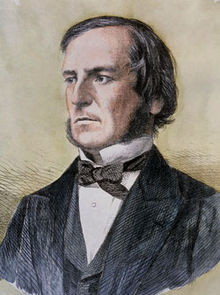
\includegraphics[width=0.9\columnwidth]{../img/boole}
\end{minipage}%
\begin{itemize}


\item Sammansatta logiska uttryck med logiska operatorer:\\
\code{&&} och, \texttt{||} eller, \texttt{!} icke, \code{==} likhet, \code{!=} olikhet,
relationer: \code{> < >= <=}

\item Exempel:
\begin{itemize}
\item[] \code{true && true}
\item[] \code{false || true}
\item[] \code{!false}
\item[] \code{42 == 43}
\item[] \code{42 != 43}
\item[] \code{(42 >= 43) || (1 + 1 == 2)}
\end{itemize}

\end{itemize}
\end{Slide}

\begin{Slide}{De Morgans lagar}

\href{https://en.wikipedia.org/wiki/Augustus_De_Morgan}{\Emph{De Morgans lagar}} beskriver vad som händer om man \Alert{negerar} ett logiskt uttryck. Kan användas för att göra \Emph{förenklingar}.

%$p$ och $q$ är logiska uttryck, $\neg$ står för ''icke'', $\wedge$ för ''och'', $\vee$ för ''eller'':
%\begin{eqnarray*}
%\neg (p \wedge q) & \Longleftrightarrow & (\neg p) \vee (\neg q)\\
%\neg (p \vee q) & \Longleftrightarrow & (\neg p) \wedge (\neg q)\\
%\end{eqnarray*}

\begin{itemize}
\item I all deluttryck sammanbundna med \code{&&} eller \code{||}, \\ ändra alla \code{&&} till \code{||} och omvänt.
\item Negera alla ingående deluttryck. En relation negeras genom att man byter \texttt{==} mot \texttt{!=}, \texttt{<} mot \texttt{>=}, etc.
\end{itemize}

Exempel på förenkling där de Morgans lagar används upprepat:

\begin{Code}[escapechar=X,backgroundcolor=,frame=none,basicstyle=\ttfamily\fontsize{10}{12}\selectfont]
! (a < b || (a == 1 && b == 1))             X$\iff$X
! (a < b) && ! (a == 1 && b == 1)           X$\iff$X
! (a < b) && (! (a == 1) || ! (b == 1))     X$\iff$X
a >= b && (a != 1 || b != 1)
\end{Code}
\end{Slide}

\begin{Slide}{Alternativ med if-uttryck}
\begin{itemize}
\item Ett if-uttryck börjar med nyckelordet \code{if}, följt av ett logiskt uttryck inom parentes och två grenar.
\begin{Code}
def slumpgrönsak = if (math.random() < 0.8) "gurka" else "tomat"
\end{Code}
\item Den ena grenen evalueras om uttrycket är \code{true}
\item Den andra \code{else}-grenen evalueras om uttrycket är \code{false}
\begin{REPLnonum}
scala> slumpgrönsak
res13: String = gurka

scala> slumpgrönsak
res14: String = gurka

scala> slumpgrönsak
res15: String = tomat

\end{REPLnonum}
\end{itemize}
\end{Slide}

\Subsection{Satser}


%%%%%%%%%%%%%%%%%%%%%%%%
\begin{Slide}{Variabeldeklaration och tilldelningssats}\SlideFontTiny

\begin{itemize}
\item En \Emph{variabeldeklaration} medför att \Alert{plats i datorns minne} reserveras så att värden av den typ som variabeln kan referera till får plats där.

\item Vid deklaration ska variabeln \Emph{initialiseras} med ett startvärde.

\item En \code{val}-deklaration ger en variabel som efter initialisering inte kan ändras.


\begin{multicols}{2}
Dessa deklarationer...
\begin{lstlisting}
var x = 42
val y = x + 1
\end{lstlisting}
... ger detta innehåll någonstans i minnet:

%http://tex.stackexchange.com/questions/18521/tikz-matrix-as-a-replacement-for-tabular
\begin{tikzpicture}[]
\matrix [matrix of nodes, row sep=0, column 2/.style={nodes={rectangle,draw,minimum width=3em}}]
{
x   & 42 \\
y   & 43 \\
};
\end{tikzpicture}
%\end{column}

%\end{columns}

\end{multicols}


\item Med en \Emph{tilldelningssats} ges en tidigare \code{var}-deklarerad variabel ett nytt värde:
\begin{lstlisting}
x = 13
\end{lstlisting}

\item Det gamla värdet försvinner för alltid och det nya värdet lagras istället: \\
\begin{tikzpicture}[]
\matrix [matrix of nodes, row sep=0, column 2/.style={nodes={rectangle,draw,minimum width=3em}}]
{
x   & 13 \\
y   & 43 \\
};
\end{tikzpicture}

Observera att \code{y} här inte påverkas av att x ändrade värde.
\end{itemize}
\end{Slide}

\begin{Slide}{Tilldelningssatser är \emph{inte} matematisk likhet}\SlideFontSmall

\begin{itemize}

\item Likhetstecknet används alltså för att \Emph{tilldela} variabler nya värden och det är \Alert{inte} samma sak som matematisk likhet. Vad händer här?
\begin{lstlisting}
x = x + 1
\end{lstlisting}

\item Denna syntax är ett arv från de gamla språken C, Fortran mfl.

\item I \href{https://en.wikipedia.org/wiki/Assignment_(computer_science)}{andra språk} används  t.ex.  \\\vspace{1em}
\texttt{x := x + 1}  \hspace{2em} eller  \hspace{2em} \texttt{x <- x + 1} \\\vspace{0.5em}

\item Denna syntax visar kanske bättre att tilldelning är en \Emph{stegvis process}:

\begin{enumerate}\SlideFontTiny
\item Först beräknas \Emph{uttrycket till höger} om tilldelningstecknet.
\item Sedan \Emph{ersätts värdet} som variabelnamnet refererar till av det beräknade uttrycket. Det gamla värdet \Alert{försvinner för alltid}.
\end{enumerate}

\end{itemize}

\end{Slide}


\begin{Slide}{Förkortade tilldelningssatser}
\begin{itemize}
\item Det är vanligt att man vill tilldela en variabel ett nytt värde som beror av det gamla, så som i \\\code{x = x + 1}

\item Därför finns \Emph{förkortade tilldelningssatser} som gör så att man sparar några tecken och det blir tydligare (?) vad som sker (när man vant sig vid detta skrivsätt):
\begin{Code}
x += 1
\end{Code}

\item Uttrycket ovan expanderas av kompilatorn till \code{x = x + 1}
\end{itemize}


\end{Slide}


\begin{Slide}{Exempel på förkortade tilldelningssatser}
\begin{REPLnonum}
scala> var x = 42
x: Int = 42

scala> x *= 2

scala> x
res0: Int = 84


scala> x /= 3

scala> x
res2: Int = 28
\end{REPLnonum}
\end{Slide}


\ifkompendium\else
\begin{Slide}{Övning: Tilldelningar i sekvens}\footnotesize

%\begin{columns}
%\begin{column}{0.32\textwidth}
\begin{minipage}{0.32\textwidth}

Rita hur minnet ser ut efter varje rad nedan:
\vskip1em
\begin{lstlisting}[ numbers=left,]
var u = 42
var x = 10
var y = 2 * x + 1
x = 20
var z = y + x + y - x
x += 1; y *= 2
\end{lstlisting}
%\end{column}
\end{minipage}\hspace{2em}%
%\begin{column}{0.6\textwidth}
\begin{minipage}{0.6\textwidth}


\scriptsize En variabel som ännu inte \Emph{initierats} har ett \Alert{odefinierat} värde, anges nedan med frågetecken.
\begin{table}[]
\centering\scriptsize
%http://tex.stackexchange.com/questions/83930/what-are-the-different-kinds-of-boxes-in-latex
\newcommand{\mybox}[1]{\raisebox{-0.5mm}{\framebox(21,14){#1}}\vspace{0.5mm}}
\begin{tabular}{@{}ccccccc}
 & rad 1 & rad 2 & rad 3 & rad 4  & rad 5 & rad 6\\
u& \mybox{42 } &  \mybox{}   &   \mybox{}   & \mybox{} & \mybox{} & \mybox{} \\
x& \mybox{? } &  \mybox{}   &   \mybox{}   & \mybox{} & \mybox{}  & \mybox{} \\
y& \mybox{? } &  \mybox{}   &   \mybox{}   & \mybox{} & \mybox{}  & \mybox{} \\
z& \mybox{? } &  \mybox{}   &   \mybox{}   & \mybox{} & \mybox{}  & \mybox{} \\
\end{tabular}
\end{table}

%\end{column}
%\end{columns}
\end{minipage}%
\end{Slide}
\fi



\begin{Slide}{Variabler som ändrar värden kan vara knepiga}
\begin{itemize}
\item Kod som innehåller variabler som \Alert{förändras} över tid är ofta svårare att läsa och begripa.

\item Många buggar beror på att variabler av misstag förändras på felaktiga och oanade sätt.

\item Föränderliga värden blir speciellt svåra i kod som körs jämlöpande (parallellt).

\item I kod som körs i skarpt läge med många användare (s.k. produktionskod) är därför \code{val} att föredra, medan \code{var} endast används om det \Alert{verkligen} behövs.
\item Alltså: räkna hellre ut nya värden än förändra befintliga.
\end{itemize}
\end{Slide}
%%%%%%%%%%



\begin{Slide}{Kontrollstrukturer: alternativ och repetition}\SlideFontSmall
Används för att kontrollera (förändra) sekvensen och skapa \Emph{alternativa} vägar genom koden. Vägen  bestäms vid körtid.
\begin{itemize}
\item if-sats:
\begin{Code}
if (math.random() < 0.8) println("gurka") else println("tomat")
\end{Code}
\end{itemize}

Olika sorters \Emph{loopar} för att repetera satser. Antalet repetitioner ges vid körtid.
\begin{itemize}
\item \code{while}-sats: bra när man \Alert{inte vet hur många gånger} det kan bli.
\begin{Code}
while (math.random() < 0.8) println("gurka")
\end{Code}

\item \code{for}-sats: bra när man \Alert{vill ange antalet repetitioner}:
\begin{Code}
for (i <- 1 to 10) println(s"gurka nr $i")
\end{Code}

\end{itemize}
\end{Slide}

%%%% GE mer detaljer eller överlåta till övning???
%\begin{Slide}{if-sats}
%\begin{itemize}
%\item
%\end{itemize}
%\end{Slide}
%
%\begin{Slide}{while-sats}
%\begin{itemize}
%\item
%\end{itemize}
%\end{Slide}
%
%\begin{Slide}{for-sats}
%\begin{itemize}
%\item
%\end{itemize}
%\end{Slide}

\begin{Slide}{Procedurer}\SlideFontSmall
\begin{itemize}
\item En \Emph{procedur} är en funktion som \Alert{gör} något intressant, men som \Alert{inte} lämnar något intressant returvärde.
\item Exempel på procedur i standardbiblioteket: \code{println("hej")}
\item Du \Emph{deklarerar egna procedurer} genom att ange \texttt{\Alert{Unit}} som returvärdestyp. Då returneras värdet \texttt{\Alert{()}} som betyder ''inget''.
\end{itemize}
\begin{REPLnonum}
scala> def hej(x: String): Unit = println(s"Hej på dej $x!")
hej: (x: String)Unit

scala> hej("Herr Gurka")
Hej på dej Herr Gurka!

scala> val x = hej("Fru Tomat")
Hej på dej Fru Tomat!
x: Unit = ()
\end{REPLnonum}
\begin{itemize}
\item Det som \Alert{görs} kallas (sido)\Emph{effekt}. Ovan är utskriften själva effekten.
\item Även funktioner kan ha sidoeffekter. De kallas då \Alert{oäkta} funktioner.
\end{itemize}
\end{Slide}

\begin{Slide}{Problemlösning: nedbrytning i abstraktioner som sen kombineras}\SlideFontSmall
\begin{itemize}
\item En av de allra viktigaste principerna inom programmering är \Emph{funktionell nedbrytning} där  \Emph{underprogram} i form av funktioner och procedurer skapas för att bli byggstenar som kombineras till mer avancerade funktioner och procedurer.

\item Genom de namn som definieras skapas \Emph{återanvändbara abstraktioner} som kapslar in det funktionen gör till ett ''byggblock''.

\item Bra ''byggblock'' gör det lättare att lösa svåra programmeringsproblem.

\item Abstraktioner som beräknar eller gör \Emph{en enda, väldefinierad sak} är enklare att använda, jämfört med de som gör många, helt olika saker.

\item Abstraktioner med \Emph{välgenomtänkta namn} är enklare att använda, jämfört med kryptiska eller missvisande namn.
\end{itemize}

\end{Slide}

\ifkompendium\else

\begin{SlideExtra}{Om veckans övning: \code{expressions}}\SlideFontSmall

\begin{itemize}
%!TEX encoding = UTF-8 Unicode

\item Förstå vad som händer när satser exekveras och uttryck evalueras.
\item Förstå sekvens, alternativ och repetition.
\item Känna till literalerna för enkla värden, deras typer och omfång.
\item Kunna deklarera och använda variabler och tilldelning, samt kunna rita bilder av minnessituationen då variablers värden förändras.
\item Förstå skillnaden mellan olika numeriska typer, kunna omvandla mellan dessa och vara medveten om noggrannhetsproblem som kan uppstå.
\item Förstå booleska uttryck och värdena \code{true} och \code{false}, samt kunna förenkla booleska uttryck.
\item Förstå skillnaden mellan heltalsdivision och flyttalsdivision, samt användning av rest vid heltalsdivision.
\item Förstå precedensregler och användning av parenteser i uttryck.
\item Kunna använda \code{if}-satser och \code{if}-uttryck.
\item Kunna använda \code{for}-satser och \code{while}-satser.
\item Kunna använda \code{math.random()} för att generera slumptal i olika intervaller.
\item Kunna beskriva skillnader och likheter mellan en procedur och en funktion.

\end{itemize}

\end{SlideExtra}

\begin{SlideExtra}{Om veckans labb: \code{kojo}}
\begin{itemize}
%!TEX encoding = UTF-8 Unicode

\item Kunna kombinera principerna sekvens, alternativ, repetition, och abstraktion i skapandet av egna program om minst 20 rader kod.
\item Kunna förklara vad ett program gör i termer av sekvens, alternativ, repetition, och abstraktion.
\item Kunna tillämpa principerna sekvens, alternativ, repetition, och abstraktion i enkla algoritmer.
\item Kunna formatera egna program så att de blir lätta att läsa och förstå.
\item Kunna förklara vad en variabel är och kunna skriva deklarationer och göra tilldelningar.
\item Kunna genomföra upprepade varv i cykeln \emph{editera-exekvera-felsöka/förbättra} för att successivt bygga upp allt mer utvecklade program.

\end{itemize}
\end{SlideExtra}

\fi

%%%%%%%%%%%%%%%%%%%%%%%%%%%%%%%%%%%%%% nedan redan meddelat i introveckan
%\ifkompendium\else
%\Subsection{Meddelande från \href{http://lth.se/code}{Code@LTH}}
%\fi


\Lecture{2}{Kodstrukturer}
%!TEX encoding = UTF-8 Unicode
%!TEX root = ../lect-w02.tex

\Subsection{Datastrukturer}

\begin{Slide}{Vad är en datastruktur?}\SlideFontSmall
\begin{itemize}
\item En \href{https://sv.wikipedia.org/wiki/Datastruktur}{datastruktur} är en struktur för organisering av data som...
\begin{itemize}\SlideFontTiny
\item kan innehålla \Alert{många} element,
\item kan refereras till som en helhet, och
\item ger möjlighet att komma åt enskilda element.
\end{itemize}

\item En \Emph{samling} \Eng{collection} är en datastruktur som kan innehålla många element av \Alert{samma typ}.

\item Exempel på olika samlingar där elementen är organiserade på olika vis: \\
\vspace{0.5em}
\begin{tabular}{l c}
\Emph{Sekvens} & 
\includegraphics[width=5cm]{../img/list.pdf} \\
\Emph{Träd}  & 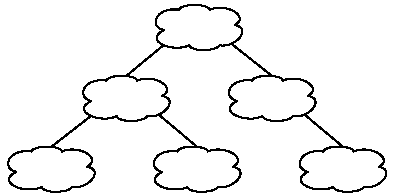
\includegraphics[width=2.2cm]{../img/tree.pdf} \\
\Emph{Graf}  & 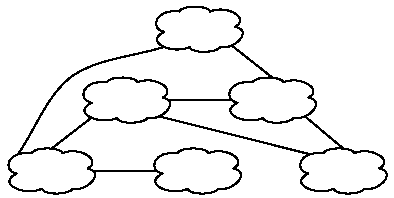
\includegraphics[width=2.2cm]{../img/graph.pdf} \\
\end{tabular}
\end{itemize}
{
\SlideFontTiny \vspace{1em }\hskip2em
Mer om sekvenser \& träd i \href{http://cs.lth.se/edaa01vt}{EDAA01 pfk}.
Mer om träd, grafer i \href{http://cs.lth.se/edaa40}{Diskreta strukturer.}
}

\end{Slide}




\begin{Slide}{Några samlingar i \texttt{scala.collection}}\SlideFontSmall
\setlength{\leftmargini}{0pt}
\begin{itemize}
\item En \Emph{samling} \Eng{collection} är en datastruktur som kan innehålla många element av \Alert{samma typ}.
\item En \Emph{sekvens} \Eng{sequence} är en samling där alla element är ordnade.

\item Exempel på \Emph{färdiga samlingar} i Scalas standardbibliotek där elementen är organiserade  internt på \Alert{olika} vis så att samlingen får olika egenskaper som passar \Alert{olika användningsområden}:
\begin{itemize}\SlideFontTiny
\item \texttt{scala.collection.immutable.\Emph{Vector}}, sekvens med snabb access \Alert{överallt}.
\item \texttt{scala.collection.immutable.\Emph{List}}, sekvens med snabb access \Alert{i början}.
\item \texttt{scala.collection.immutable.\Emph{Set}}, \texttt{scala.collection.\Alert{mutable}.\Emph{Set}}, mängd med unika element; ej i sekvens men snabb innehållstest.
\item \texttt{scala.collection.immutable.\Emph{Map}}, \texttt{scala.collection.\Alert{mutable}.\Emph{Map}}, mängd med par av nyckel \& tillhörande värde, snabb access via nyckel.
\item \texttt{scala.collection.\Alert{mutable}.\Emph{ArrayBuffer}}, förändringsbar sekvens kan ändra storlek.
\item \texttt{scala.\Emph{Array}}, förändringsbar sekvens som \Alert{inte} kan ändra storlek. Alla element är lagrade efter varandra i minnet: snabbast access av alla samlingar.
\end{itemize}
\end{itemize}
\end{Slide}


\begin{Slide}{Olika sätt att skapa datastrukturer}
\begin{itemize}
\item \Emph{Tupel} \Eng{tuple}
  \begin{itemize}
  \item samla $n$ st datavärden i element \Emph{\code{_1}}, \Emph{\code{_2}}, ...  \code{_}$n$
  \item elementen kan vara av \Alert{olika} typ
  \end{itemize}
\item \Emph{Klass} \Eng{class}
  \begin{itemize}
  \item samlar data i \Emph{attribut} med (väl valda!) namn
  \item attributen kan vara av \Alert{olika} typ
  \item definierar även \Emph{metoder} som använder attributen \\ (kallas även \Emph{operationer} på data)
  \end{itemize}

\item \Emph{Färdig samling}
  \begin{itemize}
  \item speciella klasser som samlar data i element av \Alert{samma} typ
  \item exempel: \code{scala.collection.immutable.Vector}
  \item har ofta \emph{många} färdiga \Emph{bra-att-ha-metoder}, \\ se snabbreferensen \url{http://cs.lth.se/pgk/quickref}
  \end{itemize}

\item \Emph{Egenimplementerade samlingar}
  \begin{itemize}
  \item $\rightarrow$ fördjupningskurs
  \end{itemize}

\end{itemize}
\end{Slide}





\begin{Slide}{Vad är en vektor?}\SlideFontSmall
En \Emph{vektor}\footnote{Vektor kallas ibland på svenska även \href{https://sv.wikipedia.org/wiki/F\%C3\%A4lt_\%28datastruktur\%29}{fält}, men det skapar stor förvirring eftersom det engelska ordet \emph{field} ofta används för \emph{attribut} (förklaras senare).}
\Eng{vector} är en \Emph{sekvens} som är \Alert{snabb} att \Emph{indexera} i.
Åtkomst av element i en sekvens som t.ex. heter \code{xs} sker i Scala med \code{xs.apply(platsnummer)}:

\begin{REPL}
scala> val heltal = Vector(42, 13, -1, 0, 1)
heltal: scala.collection.immutable.Vector[Int] = Vector(42, 13, -1, 0, 1)

scala> heltal.apply(0)   // platsnummer räknas från noll
res0: Int = 42

scala> heltal(1)         // man kan i Scala skippa .apply före (
res1: Int = 13

scala> heltal(5)         // ger körtidsfel då sjätte platsen inte finns
java.lang.IndexOutOfBoundsException: 5
  at scala.collection.immutable.Vector.checkRangeConvert(Vector.scala:132)
\end{REPL}
Utelämnar du \code{.apply} så skapar kompilatorn automatiskt ett anrop av \code{apply}.
\end{Slide}

\begin{Slide}{En konceptuell bild av en vektor}

\begin{REPLnonum}
scala> val heltal = Vector(42, 13, -1, 0, 1)

scala> heltal(0)
res0: Int = 42
\end{REPLnonum}

\begin{tikzpicture}[font=\ttfamily]
\matrix [matrix of nodes, row sep=0, column 2/.style={nodes={rectangle,draw,minimum width=3em}}] (var) at (0cm, 2.8cm)
{
heltal   &  \makebox(16,12){ }\\
};
\matrix [matrix of nodes, draw=black,row sep=0, column 2/.style={nodes={rectangle,draw,minimum width=4em}}] (vec) at (4cm, 1cm)
{
\textit{plats} &  \\
0   &  \makebox(16,12){42}\\
1   &  \makebox(16,12){13}\\
2   &  \makebox(16,12){-1}\\
3   &  \makebox(16,12){0}\\
4   &  \makebox(16,12){1}\\
};
\filldraw[black] (0.7cm,2.8cm) circle (3pt) node[] (ref) {};
 \draw [arrow] (ref) -- (vec);
\end{tikzpicture}

%\vspace{1em} Elementen ligger på rad någonstans i minnet.
\end{Slide}



\begin{Slide}{En samling strängar}

\begin{itemize}
\item En vektor kan lagra många värden av samma typ.
\item Elementen kan vara till exempel heltal eller strängar.
\item Eller faktiskt vad som helst. (En s.k. \emph{generisk} samling.)
\end{itemize}

\begin{REPL}
scala> val grönsaker = Vector("gurka","tomat","paprika","selleri")
grönsaker: scala.collection.immutable.Vector[String] =
  Vector(gurka, tomat, paprika, selleri)

scala> val g = grönsaker(1)
g: String = tomat

scala> val xs = Vector(42, "gurka", true, 42.0)
xs: scala.collection.immutable.Vector[Any] = Vector(42, gurka, true, 42.0)
\end{REPL}
Notera typen \code{Any} som betyder ''\Emph{vilken typ som helst}''. \footnote{(\code{Any} liknar Java's \code{Object} men är \Alert{mer generell}; mer om \code{Any} senare).}
\end{Slide}



\Subsection{Kontrollstrukturer}


\begin{Slide}{Vad är en kontrollstruktur?}
\begin{itemize}
\item En \Emph{kontrollstruktur} påverkar \Alert{sekvensen}.
\begin{itemize}
\item[] Exempel på inbyggda kontrollstrukturer:
\\\vspace{0.5em}\code{for}-sats, \code{while}-sats, \code{for}-\code{yield}-uttryck
\end{itemize}

\item[]

\item I Scala kan man definiera \Emph{egna} kontrollstrukturer.
\begin{itemize}
\item[] Exempel: \code{upprepa} som du använt i Kojo
\\\vspace{0.5em}\code|upprepa(4){fram; höger}|
\end{itemize}
\end{itemize}
\end{Slide}

\ifkompendium\else
\begin{Slide}{Mitt första program: en oändlig loop på ABC80}
\begin{minipage}{0.8\textwidth}
\begin{verbatim}
10 print "hej"
20 goto 10
\end{verbatim}
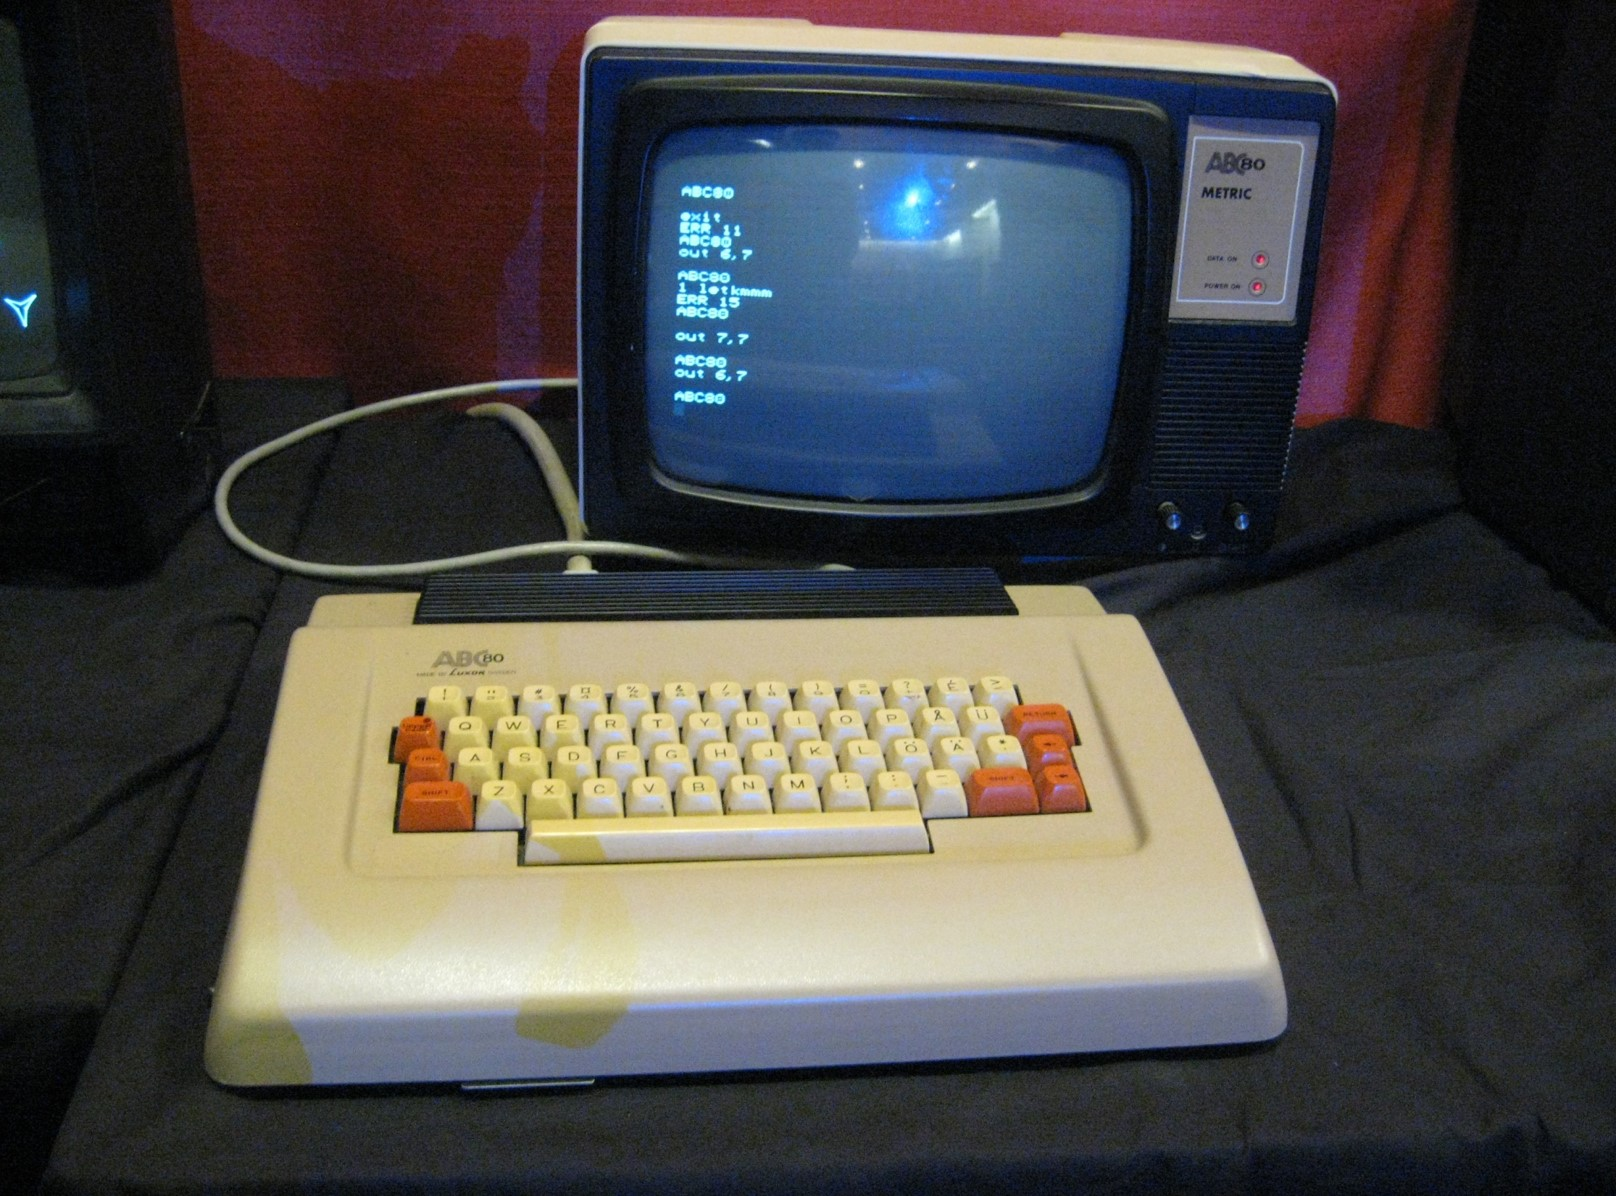
\includegraphics[width=0.8\textwidth]{../img/abc80.jpg}
\end{minipage}%
\begin{minipage}{0.2\textwidth}
\pause
\begin{verbatim}
hej
hej
hej
hej
hej
hej
hej
hej
hej
hej
hej
hej
<Ctrl+C>
\end{verbatim}
\end{minipage}
\end{Slide}
\fi

\begin{Slide}{Loopa genom elementen i en vektor}
En \code{for}-\Emph{sats} som skriver ut alla element i en vektor:
\begin{REPL}
scala> val grönsaker = Vector("gurka","tomat","paprika","selleri")

scala> for (g <- grönsaker) println(g)
gurka
tomat
paprika
selleri

\end{REPL}
Den stiliserade bakåtpilen \code{<-} betyder:\\Plocka ut varje element ur samlingen och låt namnet före pilen (här \code{g}) referera till ett nytt värde för varje runda i loopen.\\Detta namn motsvarar en \Emph{lokal} \code{val}-variabel.
\end{Slide}


\begin{Slide}{Bygg ny samling från befintlig med for-yield-uttryck}
Ett \code{for}-\code{yield}-\Emph{uttryck} som \Emph{skapar en \Alert{ny} samling}.

\begin{Code}[basicstyle=\ttfamily\fontsize{12}{14}\selectfont]
for (g <- grönsaker) yield "god " + g
\end{Code}

\begin{REPL}
scala> val grönsaker = Vector("gurka","tomat","paprika","selleri")

scala> val åsikter = for (g <- grönsaker) yield "god " + g
åsikter: scala.collection.immutable.Vector[String] =
  Vector(god gurka, god tomat, god paprika, god selleri)
\end{REPL}

\end{Slide}


\begin{Slide}{Samlingen \code{Range} håller reda på intervall}
\begin{itemize}
\item Med en \code{Range(start, slut)} kan du skapa ett intervall: \\ från och med \code{start} till (men inte med) \code{slut}
\end{itemize}

\begin{REPLnonum}
scala> Range(0, 42)
res0: scala.collection.immutable.Range =
  Range(0, 1, 2, 3, 4, 5, 6, 7, 8, 9, 10, 11, 12, 13, 14,
    15, 16, 17, 18, 19, 20, 21, 22, 23, 24, 25, 26, 27, 28,
    29, 30, 31, 32, 33, 34, 35, 36, 37, 38, 39, 40, 41)
\end{REPLnonum}

\begin{itemize}
\item Men alla värden däremellan skapas inte förrän de behövs:
\end{itemize}

\begin{REPL}
scala> val jättestortIntervall = Range(0, Int.MaxValue)
jättestortIntervall: scala.collection.immutable.Range = Range(0, 1, 2, 3, 4, 5, ...

scala> jättestortIntervall.end
res1: Int = 2147483647

scala> jättestortIntervall.toVector
java.lang.OutOfMemoryError: GC overhead limit exceeded
\end{REPL}

\end{Slide}

\begin{Slide}{Loopa med Range}
\code{Range} används i for-loopar för att hålla reda på antalet rundor.
\begin{REPLnonum}
scala> for (i <- Range(0, 6)) print(" gurka " + i)
 gurka 0 gurka 1 gurka 2 gurka 3 gurka 4 gurka 5
\end{REPLnonum}
Du kan skapa en \code{Range} med \code{until} efter ett heltal:
\begin{REPLnonum}
scala> 1 until 7
res1: scala.collection.immutable.Range =
  Range(1, 2, 3, 4, 5, 6)

scala> for (i <- 1 until 7) print(" tomat " + i)
 tomat 1 tomat 2 tomat 3 tomat 4 tomat 5 tomat 6

\end{REPLnonum}
\end{Slide}

\begin{Slide}{Loopa med Range skapad med \texttt{to}}

Med \code{to} efter ett heltal får du en \code{Range} till och \Emph{med} sista:
\begin{REPLnonum}
scala> 1 to 6
res2: scala.collection.immutable.Range.Inclusive =
  Range(1, 2, 3, 4, 5, 6)

scala> for (i <- 1 to 6) print(" gurka " + i)
 gurka 1 gurka 2 gurka 3 gurka 4 gurka 5 gurka 6

\end{REPLnonum}


\end{Slide}



\begin{Slide}{Vad är en \code{Array} i JVM?}


\begin{itemize}
\item En \href{https://en.wikipedia.org/wiki/Array_data_structure}{\code{Array}} liknar en \code{Vector} men har en särställning i JVM:
\begin{itemize}
\item Lagras som en sekvens i minnet på efterföljande adresser.
\item \Emph{Fördel}: snabbaste samlingen för element-access i JVM.
\item Men det finns en hel del \Alert{nackdelar} som vi ska se senare.
\end{itemize}

\end{itemize}

\begin{REPLnonum}
scala> val heltal = Array(42, 13, -1, 0 , 1)
\end{REPLnonum}

\begin{tikzpicture}[font=\ttfamily,scale=0.75, every node/.style={scale=0.75}]
\matrix [matrix of nodes, row sep=0, column 2/.style={nodes={rectangle,draw,minimum width=3em}}] (var) at (0cm, 2.8cm)
{
heltal   &  \makebox(16,12){ }\\
};
\matrix [matrix of nodes, draw=black,row sep=0, column 2/.style={nodes={rectangle,draw,minimum width=4em}}] (vec) at (4cm, 1cm)
{
\textit{plats} &  \\
0   &  \makebox(16,12){42}\\
1   &  \makebox(16,12){13}\\
2   &  \makebox(16,12){-1}\\
3   &  \makebox(16,12){0}\\
4   &  \makebox(16,12){1}\\
};
\filldraw[black] (0.7cm,2.8cm) circle (3pt) node[] (ref) {};
 \draw [arrow] (ref) -- (vec);
\end{tikzpicture}
\end{Slide}

\begin{Slide}{Några likheter \& skillnader mellan \texttt{Vector} och \texttt{Array}}\SlideFontSmall
\begin{multicols}{2}
\begin{REPLnonum}
scala> val xs = Vector(1,2,3)
\end{REPLnonum}

\columnbreak

\begin{REPLnonum}
scala> val xs = Array(1,2,3)
\end{REPLnonum}
\end{multicols}


Några likheter mellan \texttt{Vector} och \texttt{Array}
\begin{itemize}
\item Båda är samlingar som kan innehålla många element.

\item Med båda kan man snabbt accessa vilket element som helst: \code{xs(2)}
\end{itemize}
Några viktiga skillnader:

\vspace{-0.5em}\begin{multicols}{2}
\Emph{Vector}
\begin{itemize}
\item Är \Emph{oföränderlig}: du kan lita på att elementreferenserna aldrig någonsin kommer att ändras.

\item Är \Emph{snabb på att skapa en delvis förändrad kopia}, t.ex. tillägg/borttagning/uppdatering mitt i sekvensen.

\end{itemize}


\columnbreak

\Alert{Array}
\begin{itemize}
\item Är \Alert{föränderlig}: \code{xs(2) = 42}

\item Är \Alert{snabb} om man bara vill läsa eller skriva på befintliga platser.

\item Är \Alert{långsam} om man vill lägga till eller ta bort element mitt i sekvensen.
\item Kan \Alert{ej} ändra storlek.

\end{itemize}
\end{multicols}
\end{Slide}



\Subsection{Huvudprogram med \texttt{main} i Scala och Java}

\begin{Slide}{Ett minimalt fristående program i Scala och Java}
Nedan Scala-kod skrivs i en editor, spara med valfritt filnamn:
\begin{Code}
// this is Scala

object Hello {
  def main(args: Array[String]): Unit = {
    println("Hejsan scala-appen!")
  }
}
\end{Code}

\pause
\vspace{1em}
Nedan Java-kod skrivs i en editor, filen \Alert{måste} heta \texttt{Hi.java}

\begin{Code}[language=Java]
// this is Java

public class Hi {
    public static void main(String[] args) {
        System.out.println("Hejsan Java-appen!");
    }
}
\end{Code}

\end{Slide}


\begin{Slide}{Loopa genom en samling med en \texttt{while}-sats}
\begin{REPLnonum}
scala> val xs = Vector("Hej","på","dej","!!!")
xs: scala.collection.immutable.Vector[String] =
  Vector(Hej, på, dej, !!!)

scala> xs.size
res0: Int = 4

scala> var i = 0
i: Int = 0

scala> while (i < xs.size) { println(xs(i)); i = i + 1 }
Hej
på
dej
!!!
\end{REPLnonum}
\end{Slide}


\begin{Slide}{Loopa genom argumenten i ett Scala-huvudprogram}
Skriv denna kod och spara i filen \texttt{helloargs.scala}
\begin{REPLnonum}
$ atom helloargs.scala
\end{REPLnonum}
\begin{Code}
object HelloScalaArgs {
  def main(args: Array[String]): Unit = {
    var i = 0
    while (i < args.size) {
      println(args(i))
      i = i + 1
    }
  }
}
\end{Code}
Kompilera och kör:
\begin{REPL}
$ scalac helloargs.scala
$ scala HelloScalaArgs hej gurka tomat
hej
gurka
tomat
\end{REPL}
\end{Slide}


\begin{Slide}{Loopa genom argumenten i ett Java-huvudprogram}
\begin{REPLnonum}
$ atom HelloJavaArgs.java
\end{REPLnonum}
\begin{Code}[language=Java]
// this is Java

public class HelloJavaArgs {
    public static void main(String[] args) {
    int i = 0;
    while (i < args.length) {
      System.out.println(args[i]);
      i = i + 1;
    }
  }
}
\end{Code}
Kompilera och kör:
\begin{REPL}
$ javac HelloJavaArgs.java
$ java HelloJavaArgs hej gurka tomat
hej
gurka
tomat
\end{REPL}

\end{Slide}


\begin{Slide}{För kännedom (överkurs): Scala-\textbf{skript}}
\begin{itemize}
\item Skala-kod kan köras som ett \Emph{skript}.\footnote{\SlideFontTiny Du får prova detta på övningen. Vi kommer mest att köra kompilerat i kursen, då Scala-skript saknar mekanism för inkludering av andra skript. Men det finns ett öppenkällkodsprojekt som löser det: \url{http://www.lihaoyi.com/Ammonite/}
}
\item Ett skript kompileras varje gång innan det körs och maskinkoden sparas inte som vid vanlig kompilering.
\item Då behövs ingen \code{main} och inget \code{object}
\end{itemize}

\begin{Code}[basicstyle=\ttfamily\fontsize{10}{12}\selectfont]
// spara nedan i filen 'myscript.scala'

println("Hej alla mina argument:")
for (arg <- args) println("Hej: " + arg)
\end{Code}

\begin{REPLnonum}
> scala myscript.scala
\end{REPLnonum}


\end{Slide}



\Subsection{Algoritmer: stegvisa lösningar}

\begin{Slide}{Vad är en algoritm?}
En \href{https://sv.wikipedia.org/wiki/Algoritm}{algoritm} är en sekvens av instruktioner som beskriver \\hur man löser ett problem.\\
\vspace{1em}
\Emph{Exempel}:
\begin{itemize}
\item	 baka en kaka
\pause\item räkna ut din pensionsprognos
\pause\item köra bil
\pause\item kolla om highscore i ett spel
\item ...
\end{itemize}

\begin{tikzpicture}[overlay]
\node[xshift=0.85\textwidth, scale=2.0] { 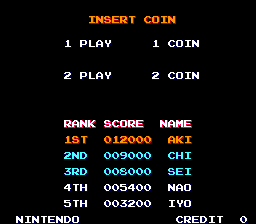
\includegraphics[width=0.25\textwidth]{../img/highscore}};
\end{tikzpicture}
\end{Slide}


\ifkompendium\else
\begin{Slide}{Algoritm-exempel: HIGHSCORE}
\Emph{Problem}: Kolla om high-score i ett spel \\ \vspace{1em}

\Emph{Varför?} \pause Så att de som spelar uppmuntras att spela mer :) \\ \vspace{1em}

\Emph{Algoritm:}\pause
\begin{enumerate}
\item $points$ $\leftarrow$ poängen efter senaste spelet
\item $highscore$ $\leftarrow$ bästa resultatet innan senaste spelet
\item \Key{om} $points$ är större än $highscore$
\begin{enumerate}[ ~~]
\item  Skriv ''Försök igen!''
\end{enumerate}
\Key{annars}
\begin{enumerate}[ ~~]
\item  Skriv ''Grattis!''
\end{enumerate}
\end{enumerate}
\pause
\scriptsize \Alert{Hittar du buggen?}

\pause Utskriften blir fel; vänd villkor eller byt plats på grenarna i if-satsen
\end{Slide}
\fi


\begin{Slide}{HIGHSCORE implementerad i Scala}
\begin{Code}
import scala.io.StdIn.readLine

object HighScore {
  def main(args: Array[String]): Unit = {
    val points = readLine("Hur mång poäng fick du?").toInt
    val highscore = readLine("Vad var highscore före senaste spelet?").toInt
    val msg = if (points > highscore) "GRATTIS!" else "Försök igen!"
    println(msg)
  }
}
\end{Code}
\SlideFontSmall %(Mer om \code{import} senare.)\\
\pause
Är det en bugg eller en feature att det står\\ \texttt{points > highscore} \\ och inte \\ \texttt{points >= highscore} \\ ?
\pause Man får ej GRATTIS om poäng == highscore vilket är tråkigt :)
\end{Slide}


\begin{Slide}{HIGHSCORE implementerad i Java}
\begin{Code}[language=Java]
import java.util.Scanner;

public class HighScore {
    public static void main(String[] args){
        Scanner scan = new Scanner(System.in);
        System.out.println("Hur många poäng fick du?");
        int points =  scan.nextInt();
        System.out.println("Vad var highscore före senaste spelet?");
        int highscore = scan.nextInt();
        if (points > highscore) {
            System.out.println("GRATTIS!");
        } else {
            System.out.println("Försök igen!");
        }
    }
}
\end{Code}
\end{Slide}


\begin{Slide}{Algoritmexempel: N-FAKULTET}
\begin{algorithm}[H]
 \SetKwInOut{Input}{Indata}\SetKwInOut{Output}{Resultat}

 \Input{heltalet $n$}
 \Output{utskrift av produkten av de första $n$ heltalen }
 ~\\
 $prod \leftarrow 1$ \\
 $i \leftarrow 2$  \\
 \While{$i \leq n$}{
  $prod \leftarrow prod * i$\\
  $i \leftarrow i + 1$
 }
 skriv ut $prod$
\end{algorithm}
\pause\vspace{1em}
\begin{itemize}\SlideFontSmall
\item Vad händer om $n$ är noll?
\item Vad händer om $n$ är ett?
\item Vad händer om $n$ är två?
\item Vad händer om $n$ är tre?
\end{itemize}
\end{Slide}

\begin{Slide}{Algoritmexempel: MIN}
\begin{algorithm}[H]
 \SetKwInOut{Input}{Indata}\SetKwInOut{Output}{Resultat}

 \Input{Array $args$ med strängar som alla innehåller heltal}
 \Output{utskrift av minsta heltalet }
 ~\\
 $min \leftarrow$ det största heltalet som kan uppkomma  \\
 $n \leftarrow $ antalet heltal \\
 $i \leftarrow 0$ \\
 \While{$i < n$}{
   $x \leftarrow args(i).toInt$ \\
   \If{( x < $min$)}{$min \leftarrow x$}
   $i \leftarrow i + 1$
 }
 skriv ut $min$
\end{algorithm}
\pause{\hfill \SlideFontTiny \Emph{Testa med indata}: \code{args = Array("2", "42", "1", "2")}}
\end{Slide}


\Subsection{Funktioner skapar struktur}

\begin{Slide}{Mall för funktionsdefinitioner}
\SlideFontSmall
\code{def} funktionsnamn(parameterdeklarationer): returtyp = uttryck

\pause\vspace{0.5em}\Emph{Exempel}:

\begin{Code}[basicstyle=\ttfamily\fontsize{9}{11}\selectfont]
def öka(i: Int): Int = i + 1
\end{Code}
\pause Returtypen kan härledas:
\begin{Code}[basicstyle=\ttfamily\fontsize{9}{11}\selectfont]
def öka(i: Int) = i + 1
\end{Code}
Men för att få hjälp av kompilatorn är det bra att ange returtyp!\\
\pause Om flera parametrar använd kommatecken. Om flera satser använd\code|{}|
\begin{Code}[basicstyle=\ttfamily\fontsize{9}{11}\selectfont]
def isHighscore(points: Int, high: Int): Boolean = {
  val highscore: Boolean = points > high
  if (highscore) println(":)") else print(":(")
  highscore
}
\end{Code}
\pause Ovan funktion har \Alert{sidoeffekten} att skriva ut en smiley.
\end{Slide}

\begin{Slide}{Bättre många små abstraktioner som gör en sak var}

\begin{Code}[basicstyle=\ttfamily\fontsize{8}{11}\selectfont]
def isHighscore(points: Int, high: Int): Boolean = points > high

def printSmiley(isHappy: Boolean): Unit =
  if (isHappy) println(":)") else print(":(")
\end{Code}

\pause\vspace{2em}
\begin{REPLnonum}
  printSmiley(isHighscore(113,99))
\end{REPLnonum}

\pause\vspace{2em} \code{isHighscore} är en \Emph{äkta funktion} som alltid ger samma svar för samma inparametrar och saknar \Alert{sidoeffekter}.

\end{Slide}



\begin{Slide}{Vad är ett block?}

\begin{itemize}
\item Ett block \Emph{kapslar in} flera satser/uttryck och ser ''utifrån'' ut som en enda sats/uttryck.

\item Ett block skapas med hjälp av klammerparenteser (''krullparenteser'')

\item [] {\fontsize{14}{18}\selectfont \code|{ uttryck1; uttryck2; ... uttryckN }|}\\~

\pause

\item I Scala (till skillnad från många andra språk) har ett block ett \Emph{värde} och är alltså ett \Emph{uttryck}.

\item Värdet ges av \Emph{sista uttrycket} i blocket.

\begin{REPLnonum}
scala> val x = { println(1 + 1); println(2 + 2); 3 + 3 }
2
4
x: Int = 6
\end{REPLnonum}


\end{itemize}

\end{Slide}

\begin{Slide}{Namn i block blir \textbf{lokala}}
Synlighetsregler:
\begin{enumerate}
\item Identifierare deklarerade inuti ett block blir \Emph{lokala}.

\item Lokala namn \Alert{överskuggar} namn i yttre block om samma.


\item Namn syns i nästlade underblock.

\end{enumerate}

\begin{REPL}
scala> { val lokaltNamn = 42; println(lokaltNamn) }
42

scala> println(lokaltNamn)
<console>:12: error: not found: value lokaltNamn
       println(lokaltNamn)

scala> { val x = 42; { val x = 76; println(x) }; println(x) }
76
42

scala> { val x = 42; { val y = x + 1; println(y) } }
43
\end{REPL}

\end{Slide}


\begin{Slide}{Parameter och argument}

Skilj på parameter och argument!
\begin{itemize}
\item En \Alert{parameter} är det deklarerade namnet som används \Alert{lokalt} i en funktion för att referera till...

\item \Emph{argumentet} som är värdet som skickas med \Emph{vid anrop} och binds till det lokala parameternamnet.

\end{itemize}


\begin{REPLnonum}
scala> val ettArgument = 42

scala> def öka(minParameter: Int) = minParameter + 1

scala> öka(ettArgument)
\end{REPLnonum}


Speciell syntax: anrop med s.k. \Emph{namngiven parameter}
\begin{REPLnonum}
scala> öka(minParameter = ettArgument)
\end{REPLnonum}

\end{Slide}

\begin{Slide}{Procedurer}\SlideFontSmall
\begin{itemize}
\item En \Emph{procedur} är en funktion som \Alert{gör} något intressant, men som \Alert{inte} lämnar något intressant returvärde.
\item Exempel på befintlig procedur: \code{println("hej")}
\item Du \Emph{deklarerar egna procedurer} genom att ange \texttt{\Alert{Unit}} som returvärdestyp. Då ges värdet \texttt{\Alert{()}} som betyder ''inget''.
\end{itemize}
\begin{REPL}
scala> def hej(x: String): Unit = println(s"Hej på dej $x!")
hej: (x: String)Unit

scala> hej("Herr Gurka")
Hej på dej Herr Gurka!

scala> val x = hej("Fru Tomat")
Hej på dej Fru Tomat!
x: Unit = ()
\end{REPL}
\begin{itemize}
\item Det som \Alert{görs} kallas (sido)\Emph{effekt}. Ovan är utskriften själva effekten.
\item Funktioner kan också ha sidoeffekter. De kallas då \Alert{oäkta} funktioner.
\end{itemize}
\end{Slide}

\begin{Slide}{''Ingenting'' \emph{är} faktiskt någonting i Scala}
\begin{itemize}
\item I många språk (Java, C, C++, ...) är funktioner som saknar värden speciella.
 Java m.fl. har speciell syntax för procedurer med nyckelordet \jcode{void}, men \Alert{inte} Scala.

\item I Scala är procedurer inte specialfall; de är vanliga funktioner som returnerar ett värde som \Emph{representerar} ingenting, nämligen () som är av typen Unit.

\item På så sätt blir procedurer inget undantag utan följer vanlig syntax och semantik precis som för alla andra funktioner.

\item Detta är typiskt för Scala: generalisera koncepten och vi slipper besvärliga undantag! \\(Men vi måste förstå generaliseringen...)


\item [] {\SlideFontSmall
\url{https://en.wikipedia.org/wiki/Void_type}
\url{https://en.wikipedia.org/wiki/Unit_type}
}

\end{itemize}

\end{Slide}

\begin{Slide}{Abstraktion: Problemlösning genom nedbrytning i enkla funktioner och procedurer som kombineras}\SlideFontSmall
\begin{itemize}
\item En av de allra viktigaste principerna inom programmering är \Emph{funktionell nedbrytning} där  \Emph{underprogram} i form av funktioner och procedurer skapas för att bli byggstenar som kombineras till mer avancerade funktioner och procedurer.

\item Genom de namn som definieras skapas \Emph{återanvändbara abstraktioner} som kapslar in det funktionen gör.

\item Problemet blir med bra byggblock lättare att lösa.

\item Abstraktioner som beräknar eller gör \Emph{en enda, väldefinierad sak} är enklare att använda, jämfört med de som gör många, helt olika saker.

\item Abstraktioner med \Emph{välgenomtänkta namn} är enklare att använda, jämfört med kryptiska eller missvisande namn.
\end{itemize}

\end{Slide}



\begin{Slide}{Exempel på \textbf{funktionell nedbrytning}}

Kojo-labben gav exempel på \Emph{funktionell nedbrytning} där ett antal abstraktioner skapas och återanvänds.

\begin{Code}
// skapa abstraktioner som bygger på varandra

def kvadrat = upprepa(4){fram; höger}

def stapel = {
  upprepa(10){kvadrat; hoppa}
  hoppa(-10*25)
}

def rutnät = upprepa(10){stapel; höger; fram; vänster}

// huvudprogram

sudda; sakta(200)
rutnät
\end{Code}
\end{Slide}


\begin{Slide}{Varför abstraktion?}
\begin{itemize}
\item Stora program behöver delas upp annars blir det mycket svårt att förstå och bygga vidare på programmet.
\item Vi behöver kunna välja namn på saker i koden \textit{lokalt}, utan att det krockar med samma namn i andra delar av koden.
\item Abstraktioner hjälper till att hantera och kapsla in komplexa delar så att de blir enklare att använda om och om igen.

\item Exempel på \Emph{abstraktionsmekanismer} i Scala och Java:
\begin{itemize}

\item \href{https://sv.wikipedia.org/wiki/Klass_\%28programmering\%29}{Klasser} är ''byggblock'' med kod som används för att skapa \href{https://sv.wikipedia.org/wiki/Objektorienterad_programmering\#Objekt}{objekt}, innehållande delar som hör ihop. \\ Nyckelord: \code{class} och \code{object}

\item \href{https://en.wikipedia.org/wiki/Method_\%28computer_programming\%29}{Metoder} är funktioner som finns i klasser/objekt och används för att lösa specifika uppgifter.  Nyckelord: \code{def}

\item \href{https://en.wikipedia.org/wiki/Java_package}{Paket} används för att organisera kodfiler i en hierarkisk katalogstruktur och skapa namnrymder. \\Nyckelord: \Key{package}

\end{itemize}

\end{itemize}
\end{Slide}


\Subsection{Katalogstruktur för kodfiler med paket}



\begin{Slide}{Källkodsfiler och klassfiler}
\begin{tikzpicture}[node distance=1.5cm]
\node (input) [startstop] {\texttt{Hello.scala}};
\node(inptext) [right of=input, text width=5cm, scale=1.2,xshift=3.5cm]{Källkodsfil};
\node (compile) [process, below of=input] {\texttt{scalac}};
\node (output) [startstop, below of=compile] {\texttt{Hello.class}};
\node(outtext) [right of=output, text width=5cm, scale=1.2,xshift=3.5cm]{\texttt{.class}-fil med byte-kod};
\node (jvm) [process, below of=output] {JVM};
\node(jvmtext) [right of=jvm, text width=5.5cm, scale=0.8,xshift=4.5cm]{\textit{Java Virtual Machine}\\Översätter till maskinkod\\ som passar din specifika CPU\\medan programmet kör};
\draw [arrow] (input) -- (compile);
\draw [arrow] (compile) -- (output);
\draw [arrow] (output) -- (jvm);
\end{tikzpicture}
\end{Slide}




\begin{Slide}{Paket}\SlideFontSmall
\begin{itemize}
\item Paket ger struktur åt kodfilerna. Bra om man har många kodfiler.

\item Byte-koden placeras av kompilatorn i kataloger enligt paketstrukturen.


\end{itemize}

\vspace{1em}
\begin{tikzpicture}[node distance=1.5cm,scale=0.8, every node/.style={transform shape}]
\node (input) [startstop] {\texttt{greeting/Hello.scala}};
\node(inptext) [right of=input, text width=4cm, scale=1.2,xshift=4.5cm]{\lstinline{package greeting}\\\lstinline{object Hello { ... }};
\node (compile) [process, below of=input] {\texttt{scalac  greeting/Hello.java}};
\node (output) [startstop, below of=compile] {\texttt{greeting/Hello.class}};
\node(outtext) [right of=output, text width=4cm, scale=1.2,xshift=4.5cm]{Paketens bytekod hamnar i katalog med samma namn som paketnamnet};
\node (jvm) [process, below of=output] {\texttt{scala greeting.Hello}};
\draw [arrow] (input) -- (compile);
\draw [arrow] (compile) -- (output);
\draw [arrow] (output) -- (jvm);
\end{tikzpicture}

{\SlideFontTiny\vspace{1em} Katalogstrukturen för källkoden måste i Java motsvara paketstrukturen, \\men inte i Scala. Dock kräver många IDE att så görs även för Scala.}
\end{Slide}

\begin{Slide}{Import}
Med hjälp av punktnotation kommer man åt innehåll i ett paket.\\
\begin{Code}
val age = scala.io.StdIn.readLine("Ange din ålder:")
\end{Code}

En \code{import}-sats...

\begin{Code}
import scala.io.StdIn.readLine
\end{Code}

...gör så att kompilatorn ''ser'' namnet, och man slipper skriva hela sökvägen till namnet:
\begin{Code}
val age = readLine("Ange din ålder:")
\end{Code}

Man säger att det importerade namnet hamnar \Emph{\textit{in scope}}.
\end{Slide}





\begin{Slide}{Jar-filer}
\texttt{jar}-filer liknar \texttt{zip}-filer och används för att packa ihop bytekod i en enda fil för enkel distribution och körning.

\vspace{2em}
\begin{tikzpicture}[node distance=1.5cm,scale=0.8, every node/.style={transform shape}]
\node (input) [startstop] {\texttt{greeting/}};
\node(inptext) [right of=input, text width=4cm, scale=1.2,xshift=4.5cm]{en katalog med filer};
\node (jar) [process, below of=input]
{\texttt{jar cvf minjarfil.jar greeting}};

\node (output) [startstop, below of=compile] {\texttt{minjarfil.jar}};

\node(outtext) [right of=output, text width=4cm, scale=1.2,xshift=4.5cm]{En jar-fil med alla filer inpackade};

\node (jvm) [process, below of=output] {\texttt{scala -cp minjarfil.jar}};

\node(outtextjvm) [right of=jvm, text width=4cm, scale=1.2,xshift=4.5cm]{Lägg jar-filen till \\ ''classpath''};
\draw [arrow] (input) -- (jar);
\draw [arrow] (jar) -- (output);
\draw [arrow] (output) -- (jvm);
\end{tikzpicture}
\end{Slide}

\Subsection{Dokumentation}

\begin{Slide}{Dokumentation}\footnotesize
För att kod ska bli begriplig för människor är det bra att dokumentera vad den gör. Det finns \Emph{tre olika sorters kommentarer} som man kan skriva direkt i Scala/Java-koden, \Alert{som kompilatorn struntar fullständigt i}:
\begin{lstlisting}
// Enradskommentarer börjar med dubbla snedstreck
//       men de gäller bara till radslut

/* Flerradskommentarer börjar med
   snedstreck-asterisk
   och slutar med asterisk-snedstreck.  */

/** Dokumentationskommentarer placeras före
 *   t.ex. en funktion och berättar vad den gör
 *   och vad eventuella parametrar används till.
 *   Börjar med snedstreck-asterisk-asterisk.
 *   Varje ny kommentarsrad börjar med asterisk.
 *   Avslutas med asterisk-stjärna.
 */
\end{lstlisting}
\end{Slide}

\begin{Slide}{scaladoc}
Programmet \texttt{scaladoc} läser källkod och skapar en webbsajt med dokumentation.

\vspace{2em}
\begin{tikzpicture}[node distance=1.5cm,scale=0.8, every node/.style={transform shape}]

\node (input) [startstop] {\texttt{greeting/}};

\node(inptext) [right of=input, text width=4cm, scale=1.2,xshift=4.5cm]{en katalog med \texttt{.scala}-filer};

\node (scaladoc) [process, below of=input]
{\texttt{scaladoc greeting/*.scala}};

\node (output) [startstop, below of=compile] {\texttt{index.html} ~~med mera...};

\node(outtext) [right of=output, text width=4cm, scale=1.2,xshift=4.5cm]{En webbsajt};


\draw [arrow] (input) -- (scaladoc);
\draw [arrow] (scaladoc) -- (output);
\end{tikzpicture}
\end{Slide}


\ifkompendium\else

\subsection{Att göra denna vecka}
%%%
\begin{Slide}{Att göra denna vecka: Förstå grundläggande kodstrukturer}

\begin{enumerate}
%\item Laborationer är \Alert{obligatoriska}.\\ Ev. sjukdom måste anmälas \Alert{före} via mejl till kursansvarig!
\item Gör övning \texttt{programs}
\item OBS! Ingen lab denna vecka w02. Använd tiden att komma ikapp om du ligger efter!
\item Träffas i samarbetsgrupper och hjälp varandra att förstå.
\item Vi har nosat på flera koncept som vi kommer tillbaka till senare: du kommer förstå mer detaljer på djupet då.
\item Om ni inte redan gjort det: \\Visa \href{https://github.com/bjornregnell/lth-eda016-2015/tree/master/assignments}{samarbetskontrakt} för handledare på resurstid.
\item \Alert{Koda på resurstiderna} och få hjälp och tips!
\end{enumerate}
\end{Slide}

\begin{Slide}{Veckans övning: \texttt{\ExeWeekTWO}}\SlideFontTiny
\vspace{-0.5em}
\setlength{\leftmargini}{0pt}
\begin{itemize}
%!TEX encoding = UTF-8 Unicode
%!TEX root = ../compendium2.tex

\item Kunna skapa samlingarna Range, Array och Vector med heltals- och strängvärden.
\item Kunna indexera i en indexerbar samling, t.ex. Array och Vector.
\item Kunna anropa operationerna size, mkString, sum, min, max på samlingar som innehåller heltal.
\item Känna till grundläggande skillnader och likheter mellan samlingarna Range, Array och Vector.
\item Förstå skillnaden mellan en for-sats och ett for-uttryck.
\item Kunna skapa samlingar med heltalsvärden som resultat av enkla for-uttryck.
\item Förstå skillnaden mellan en algoritm i pseudo-kod och dess implementation.
\item Kunna implementera algoritmerna SUM, MIN/MAX på en indexerbar samling med en \code{while}-sats.
\item Kunna köra igång enkel Scala-kod i REPL, som skript och som applikation.
\item Kunna skriva och köra igång ett enkelt Java-program.
\item Känna till några grundläggande syntaxskillnader mellan Scala och Java, speciellt variabeldeklarationer och indexering i Array.
\item Förstå vad ett block och en lokal variabel är.
\item Förstå hur nästlade block påverkar namnsynlighet och namnöverskuggning.
\item Förstå kopplingen mellan paketstruktur och kodfilstruktur.
\item Kunna skapa en jar-fil.
\item Kunna skapa dokumentation med scaladoc.

\end{itemize}
\end{Slide}

\begin{Slide}{Labb läsvecka 3:  \texttt{\LabWeekTHREE}}\SlideFontSmall
\begin{itemize}
\item Skapa ett \Emph{lagom} irriterande textspel som körs i terminalen:
\begin{itemize}\SlideFontTiny
  \item ska vara \Emph{lagom} irriterande om man \Emph{först läser koden}
  \item får gärna vara \Alert{orimligt} irriterande om man \Alert{inte läser koden}
  \item koden ska vara \Emph{lättläst} och uppdelad i \Emph{många små funktioner} med bra, förklarande funktionsnamn, parameternamn och variablenamn
\end{itemize}
\item Använd en editor, kompilera och kör i terminalen
\item Mål: skapa \Emph{eget} program med \Emph{många små funktioner} och träna på \Emph{alla begrepp} vi använt hittills. Ju fler begrepp du kan använda på olika sätt desto bättre. Fokusera på det \Alert{du} behöver träna mest på.
\item Spela varandras textspel inom din samarbetsgrupp
\item Utveckla ditt spel \Emph{stegvis} och spela varandras halvfärdiga spel i flera omgångar. Ge varandra tips om förbättringar för att spelet ska bli mer lagom irriterande på ett kul sätt och för att koden ska bli mer lättläst.
\item Skriv ner den återkoppling du fått av din grupp inför labbredovisningen.
\item Läs igenom labbuppgiften redan nu och börja fundera. Ta dig inte ''vatten över huvudet''. Ta små steg i början och ha hela tiden körbar kod.


\end{itemize}
\end{Slide}
\fi


\Lecture{3}{Funktioner}
%!TEX encoding = UTF-8 Unicode
%!TEX root = ../lect-w03.tex


% \ifkompendium\else
% \Subsection{Scala 2.12.10}

% \begin{SlideExtra}{Scala 2.12.10}
%   Den 10:e September släpptes Scala 2.12.10 med viktigaste förbättringen att filtrering i Scaladoc nu fungerar igen. 
%   \\~\\
%   \url{https://www.scala-lang.org/news/2.12.10}
%   \\~\\ Du kan gärna installera 2.12.10 om du vill, men inte nödvändigt.
%   \\~\\ När du kollar api-dokumentationen för Scalas standardbibliotek så använd denna länk:\\ 
%   \url{https://www.scala-lang.org/api/2.12.10}

% \end{SlideExtra}
% \fi

\Subsection{Vad är en funktion?}


\ifkompendium\else
\begin{SlideExtra}{Om veckans tema: Funktioner}
\begin{itemize}
  \item Funktioner är en av de viktigaste abstraktionsmekanismerna inom datavetenskapen
  \item Du kan redan massor om funktioner, bl.a. från matematiken.
  \item Denna vecka ska vi fördjupa förståelsen:
  \begin{itemize}\SlideFontSize{6}{8}
    \item överlagring
    \item enhetlig access
    \item defaultargument
    \item namngivna argument
    \item lokala funktioner
    \item funktioner som äkta värden
    \item anonyma funktioner
    \item klammerparentes vid ensam paramenter
    \item multipla parameterlistor
    \item egendefinierade kontrollstrukturer
    \item fördröjd evaluering (''call-by-name'')
    \item stegade funktioner (''Curry-funktioner'')
    \item fångad variablelrymd (''closure'')
    \end{itemize}
\end{itemize}  
\end{SlideExtra}

\begin{SlideExtra}{Om veckans tema: Funktioner}
  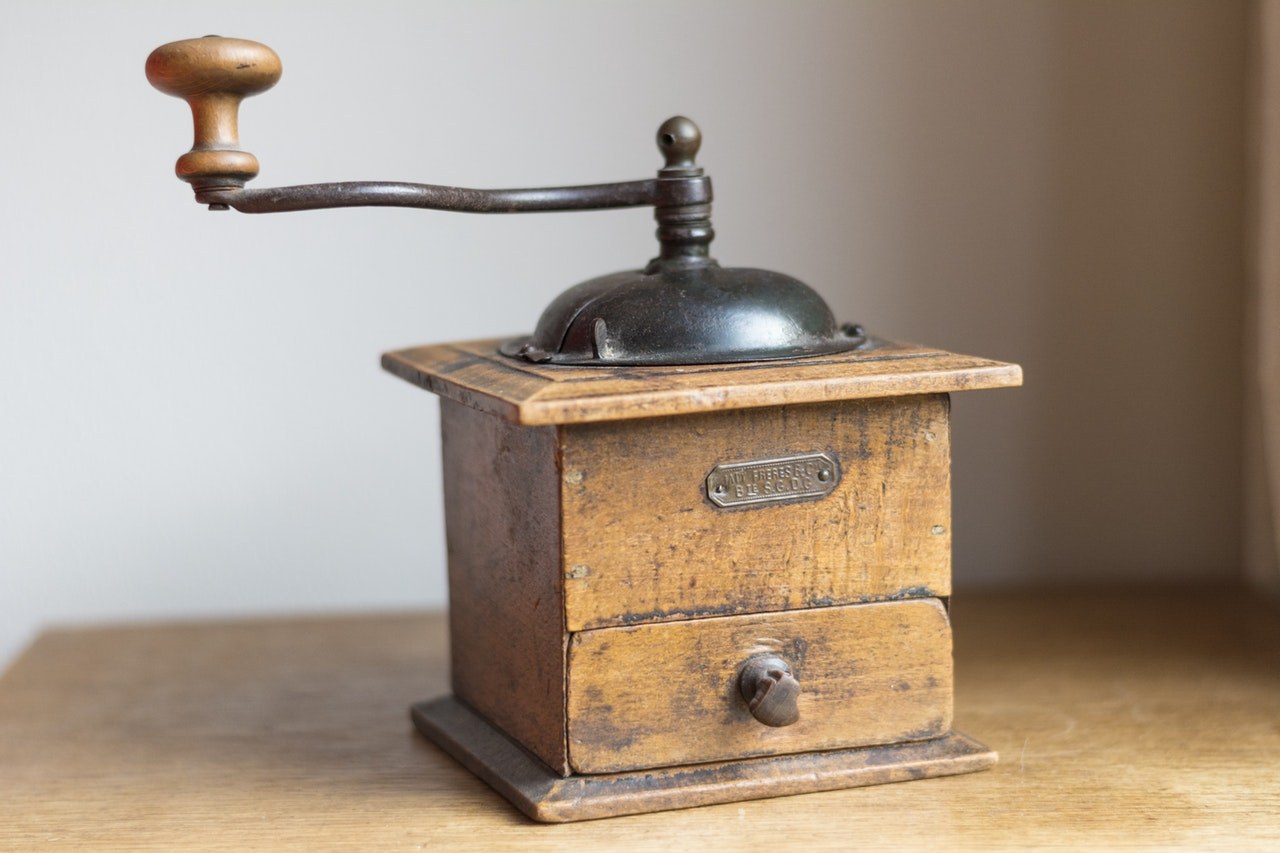
\includegraphics[width=1.0\textwidth]{../img/coffee-grinder}
\end{SlideExtra}
\fi


\begin{Slide}{Funktion: deklaration och anrop}
\SlideOnly{\setlength{\leftmargini}{0pt}}

\code{def} funktionsnamn(parameterdeklarationer): returtyp = uttryck
\vspace{0.5em}

% \begin{Code}
% def namn(param1: Typ1, param2: Typ2): Returtyp = uttryck
% \end{Code}

\begin{itemize}\SlideFontSmall
  \item En funktion har ett \Emph{huvud} och efter \code{=} kommer dess \Emph{kropp}.
  \item En \Alert{namngiven} funktion \Emph{deklareras} med nyckelordet \code{def}
  \item En funktion kan ha \Emph{parametrar} som deklareras i huvudet. 
  \item Kroppen ska vara ett uttryck (ev. ett block med flera uttryck).
  \item Parametrar binds till argument vid anrop.
  \item Uttrycket i funktionens kropp \Emph{evalueras} vid \Alert{varje anrop}. 
  \item Värdet av uttrycket blir funktionen \Emph{returvärde}. 
\end{itemize}

\pause
Exempel:
\begin{Code}
def öka(a: Int, b: Int): Int = a + b
\end{Code}
\pause
\begin{REPLnonum}
scala> öka(42, 1)
val res0: Int = 43
\end{REPLnonum}

\end{Slide}


\begin{Slide}{Deklarera funktioner, överlagring}
\begin{itemize}
\item En parameter, och sedan två parametrar:
\begin{REPL}
scala> def öka(a: Int): Int = a + 1

scala> def öka(a: Int, b: Int): Int = a + b

scala> öka(1)
val res0: Int = 2

scala> öka(1,1)
val res1: Int = 2

\end{REPL}
\item Båda funktionerna ovan kan finnas samtidigt! Trots att de har \Emph{samma namn} är de \Alert{olika funktioner}; kompilatorn kan skilja dem åt med hjälp av de \Alert{olika parameterlistorna}.

\item Detta kallas \Emph{överlagring} \Eng{overloading} av funktioner.
\item Överlagring ger flexibilitet i användningen; vi slipper hitta på nytt namn så som \code{öka2} vid 2 parametrar.
\end{itemize}
\end{Slide}



\begin{Slide}{Funktioner med defaultargument}\SlideFontSmall

\begin{itemize}
\item Vi kan ofta åstadkomma samma flexibilitet som vid överlagring, men med \Alert{en enda} funktion, om vi i stället använder \Emph{defaultargument}:
\begin{REPLnonum}
scala> def inc(a: Int, b: Int = 1) = a + b

scala> inc(42, 2)
val res0: Int = 44

scala> inc(42, 1)
val res1: Int = 43

scala> inc(42)
val res2: Int = 43

\end{REPLnonum}
\item Om ett argument utelämnas och parametern deklarerats med defaultargument så appliceras detta. Kompilatorn fyller alltså i argumentet åt oss, om det är entydigt vilken parameter som avses.
\end{itemize}
\end{Slide}


\begin{Slide}{Funktioner med namngivna argument}
\begin{itemize}
\item Genom att använda \Emph{namngivna argument} behöver man inte hålla reda på ordningen på parametrarna, bara man känner till parameternamnen.
\item Namngivna argument går fint att \Alert{kombinera} med defaultargument.
\begin{REPLnonum}[basicstyle=\SlideFontSize{7}{9}\ttfamily\color{white}]
scala> def namn(förnamn: String,
                efternamn: String,
                förnamnFörst: Boolean = true,
                ledtext: String = "Namn:"): String =
         if förnamnFörst then s"$ledtext $förnamn $efternamn"
         else s"$ledtext $efternamn, $förnamn"

scala> namn(ledtext = "Name:", efternamn = "Coder", förnamn = "Kim")
val res0: String = Name: Kim Coder
\end{REPLnonum}
\end{itemize}
\end{Slide}


\begin{Slide}{Enhetlig access}\SlideFontSmall
\begin{itemize}
\item Om en funktion \Emph{deklareras} \Alert{med} tom parameterlista \code{()} så ska den \Emph{anropas} \Alert{med} tom parameterlista.
\begin{REPLsmall}
scala> def tomParameterlista() = 42

scala> tomParameterlista()
val res1: Int = 42

scala> tomParameterlista                                                                                                                    
1 |tomParameterlista
  |^^^^^^^^^^^^^^^^^
  |method tomParameterlista must be called with () argument
\end{REPLsmall}

\item En parameterlös funktion deklarerad \Alert{utan} \code{()} ska anropas \Alert{utan} \code{()}. 
\begin{REPLsmall}
scala> def ingenParameterlista = 42
scala> ingenParameterlista()
1 |ingenParameterlista()
  |^^^^^^^^^^^^^^^^^^^
  |method ingenParameterlista does not take parameters
\end{REPLsmall}

\item Deklaration utan \code{()} möjliggör \Emph{enhetlig access}: implementationen kan ändras från \code{val} till \code{def} eller tvärtom, \Emph{utan} att \Alert{användandet} påverkas.
\pause
%\item Om parameterlista saknas får man alltså \Alert{inte} använda \code{()} vid anrop:

\end{itemize}
\end{Slide}

\Subsection{Hur ser det ut i minnet när funktioner anropas?}

\begin{Slide}{Anropsstacken och objektheapen}\SlideFontSmall
Minnet som innehåller ett programs data är uppdelat i två delar:
\begin{itemize}
\item \Emph{Anropsstacken}: 
\begin{itemize}\SlideFontSmall
\item På stackminnet läggs en \Emph{aktiveringspost} \Eng{stack frame\footnote{\href{https://en.wikipedia.org/wiki/Call_stack}{en.wikipedia.org/wiki/Call\_stack}}, activation record} för varje funktionsanrop med plats för \Alert{parametrar} och \Alert{lokala variabler}.
\item Aktiveringsposten \Alert{raderas} när \Emph{returvärdet} har levererats.
\item Stacken \Alert{växer} vid \Emph{nästlade funktionsanrop}, då en funktion i sin tur anropar en annan funktion.
\end{itemize}
\item \Emph{Objektheapen}: I heapminnet\footnote{\href{https://en.wikipedia.org/wiki/Memory_management}{en.wikipedia.org/wiki/Memory\_management}}$^{,}$\footnote{Ej att förväxlas med datastrukturen heap  \href{https://sv.wikipedia.org/wiki/Heap}{sv.wikipedia.org/wiki/Heap}} sparas alla objekt (data) som allokeras under körning. Heapen städas då och då av \Emph{skräpsamlaren} \Eng{garbage collector}, och minne som inte används längre frigörs. \\\vspace{0.5em}
%\href{http://stackoverflow.com/questions/1565388/increase-heap-size-in-java}{stackoverflow.com/questions/1565388/increase-heap-size-in-java}
% \href{https://stackoverflow.com/questions/1441373/increase-jvm-heap-size-for-scala}{stackoverflow.com/questions/1441373/increase-jvm-heap-size-for-scala}
% \begin{REPLnonum}
% scala -J-Xmx16g -J-XX:-UseGCOverheadLimit Main
% \end{REPLnonum}
\end{itemize}
\end{Slide}

% \begin{Slide}{Aktiveringspost}\SlideFontSmall
% Nästlade anrop ger växande anropsstack.
% \begin{REPL}
% scala> def f(x: Int, y: Int): Int = { val z = x + y; println(z); z}
% scala> def g(a: Int, b: Int): Int = { val c = a + b; println(c); f(c, 2 * c) }
% scala> def h(i: Int): Int = { val n = 5; g(i, i * n) }
% scala> h(2)
% \end{REPL}
%
% \pause
% \Alert{Stacken}
%
% \begin{tabular}{|r | l | l |} \hline
%
% variabel & värde & Aktiveringspost för anrop av... \\ \hline \hline
% \pause
%  i & 2 & h \\
%  n & 5 & \\ \hline
%  \pause
%  a & 2 & g \\
%  b & 10 &  \\
%  c & 12  &  \\  \hline
%  \pause
%  x & 12  & f \\
%  y & 24 &  \\
%  z & 36 & \\ \hline
% \end{tabular}
% \end{Slide}

\begin{Slide}{Aktiveringspost}\SlideFontSmall
Nästlade anrop ger växande anropsstack.
\begin{REPLsmall}
scala> def h(x: Int, y: Int) = { val z = x + y; println(z) }

scala> def g(a: Int, b: Int) = { val x = 1; h(x + 1, a + b) }

scala> def f() = { val n = 5; g(n, 2 * n) }

scala> f()

\end{REPLsmall}

\pause
\Alert{Stacken}

\begin{tabular}{|r | l | l |} \hline

variabel & värde & Aktiveringspost för anrop av... \\ \hline \hline
\pause
 n & 5 & f \\ \hline
 \pause
 a & 5 & g \\
 b & 10 &  \\
 x & 1  &  \\  \hline
 \pause
 x & 2  & h \\
 y & 15 &  \\
 z & 17 & \\ \hline
\end{tabular}
\end{Slide}

\begin{Slide}{Anropsstacken i Kojo Desktop}
Tryck på orange playknapp i Kojo och se anropsstacken.\vspace{0.5em}

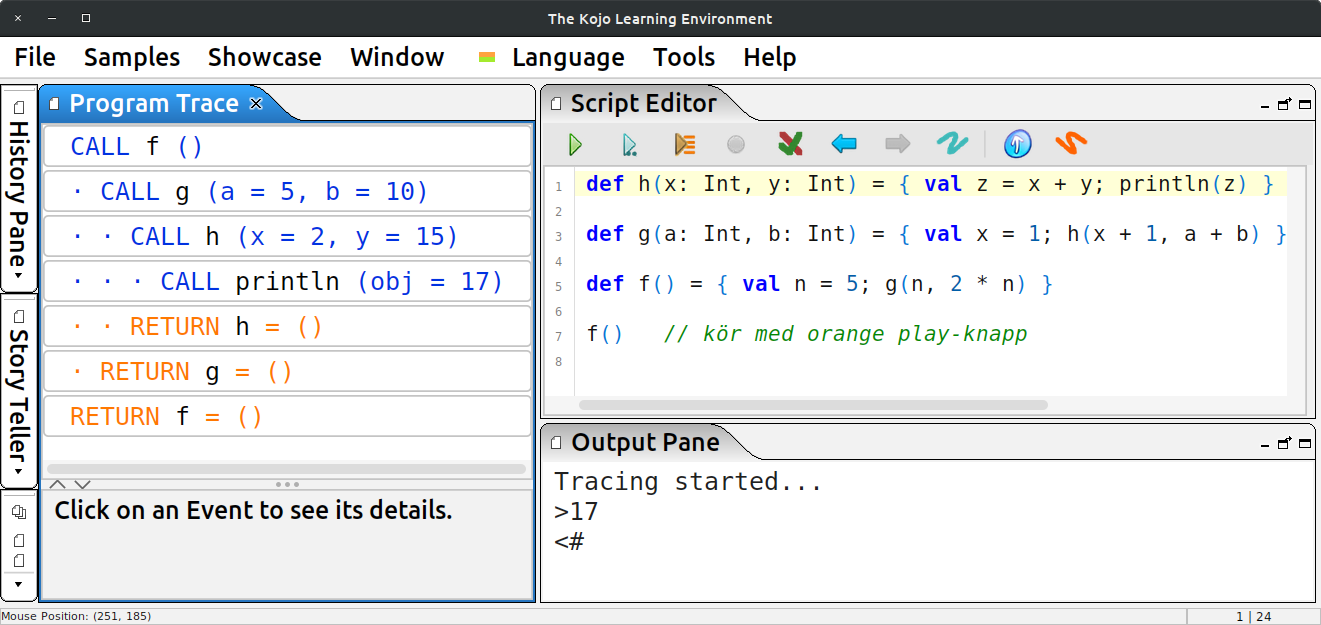
\includegraphics[width=1.0\textwidth]{../img/kojo-trace.png}  
\end{Slide}

\begin{Slide}{Anropsstacken i VS Code}
Lägg till en brytpunkt på rad 4 nedan och klicka på debug över \code{@main} i VS Code och se anropsstacken.\vspace{0.5em}

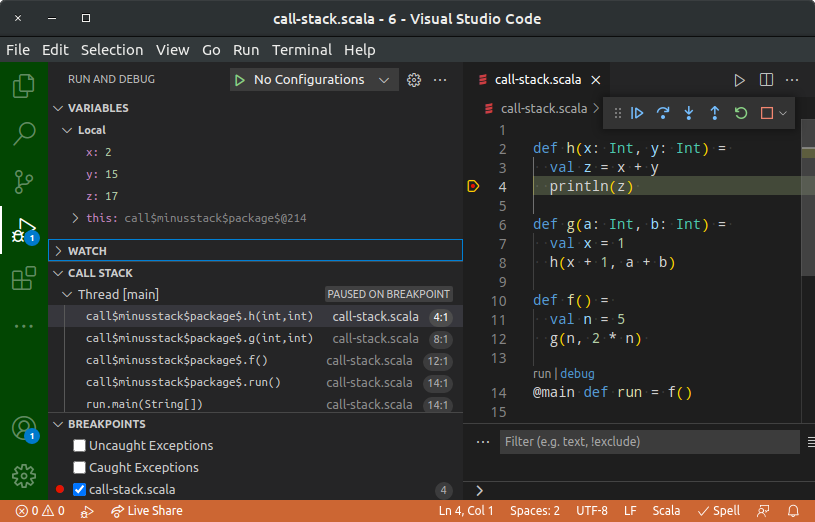
\includegraphics[width=0.85\textwidth]{../img/vscode-trace.png}  
\end{Slide}


\begin{Slide}{Vad är en stack trace?}\SlideFontSmall
När du letar buggar vid körtidsfel har du nytta av att \Alert{noga studera} \Emph{utskriften av anropsstacken} \Eng{stack trace}:
% \begin{CodeSmall}
% // Program i filen BMI.scala
% object BMI: 
%   def main(args: Array[String]): Unit = 
%     println(bmi(args(0).toInt, args(1).toInt))

%   def bmi(heightCm: Int, weightKg: Int) = 
%     safeDiv(weightKg, heightCm * heightCm) 

%   def safeDiv(numerator: Int, denominator: Int): (Int, String) = 
%     if (denominator == 0) (numerator / denominator, "ok")  // ser du buggen?
%     else (0, "division by zero") 
% \end{CodeSmall}
  
\begin{Code}[numbers=left]
// Program i filen bmi.scala

@main 
def bmi(heightCm: Int, weightKg: Int) = 
  safeDiv(weightKg, heightCm * heightCm) 

def safeDiv(numerator: Int, denominator: Int): (Int, String) = 
  if denominator == 0 then (numerator / denominator, "")  // ser du buggen?
  else (0, "division by zero")

\end{Code}
\begin{REPL}
> scalac bmi.scala 
> scala bmi 0 42
Exception in thread "main" java.lang.ArithmeticException: / by zero
        // HÄR KOMMER STACK TRACE pga körtidsfel - se nästa bild
\end{REPL}
\end{Slide}

\begin{Slide}{Hur läsa en stack trace?}
\begin{REPL}
Exception in thread "main" java.lang.ArithmeticException: / by zero
        at bmi$package$.safeDiv(bmi.scala:8)
        at bmi$package$.bmi(bmi.scala:5)
        at bmi.main(bmi.scala:3)

\end{REPL}
\begin{itemize}\SlideFontSmall
  \item En \Emph{stack trace} skrivs ut efter en krasch p.g.a. körtidsfel.
  \item Körtidsfel känns igen med ordet \Alert{Exception}.
  \item Först kommer en beskrivning av felet som orsakat kraschen, här: \\\code{java.lang.ArithmeticException: \ by zero} 
  \item Därefter visas anropsstacken.
  \item För varje funktionsanrop anges: \Emph{\texttt{klass.metod(kodfil:radnummer)}}
  \item Main-funktioner läggs i ett singelobjekt i ett speciellt paket
  \item Singelobjekt i Scala kodas som en Java-klass med dollar-tecken efter namnet, eftersom det inte finns singelobjekt i JVM.
  %\item Efter anropet av din \code{main}-procedur ligger JVM-interna anrop (\code{java.base} etc.) som du inte behöver bry dig om. %% syns inte längre i Scala 3 stack trace
\end{itemize}
\end{Slide}
  

\begin{Slide}{Lokala funktioner}\SlideFontSmall
Med lokala funktioner kan delproblem lösas med nästlade abstraktioner.

\begin{CodeSmall}
def gissaTalet(max: Int, min: Int = 1): Unit = 
  def gissat = io.StdIn.readLine(s"Gissa talet mellan $min och $max: ").toInt

  val hemlis = (math.random() * (max - min) + min).toInt

  def skrivLedtrådOmEjRätt(gissning: Int): Unit =
    if gissning > hemlis then println(s"$gissning är för stort :(")
    else if gissning < hemlis then println(s"$gissning är för litet :(")

  def inteRätt(gissning: Int): Boolean = 
    skrivLedtrådOmEjRätt(gissning)
    gissning != hemlis
  

  def loop: Int = { var i = 1; while inteRätt(gissat) do i += 1; i }

  println(s"Du hittade talet $hemlis på $loop gissningar :)")
\end{CodeSmall}

Lokala, nästlade funktionsdeklarationer är tyvärr inte tillåtna i många andra språk, t.ex. Java.\footnote{\href{http://stackoverflow.com/questions/5388584/does-java-support-inner-local-sub-methods}{\SlideFontSize{8}{9}stackoverflow.com/questions/5388584/does-java-support-inner-local-sub-methods}}

\end{Slide}

\Subsection{En funktion är ett värde}

\begin{Slide}{Funktioner är äkta värden i Scala}\SlideFontSmall
\begin{itemize}
\item En funktion är ett \Alert{äkta värde}.
\item Vi kan till exempel tilldela en variabel ett funktionsvärde.
\pause
\item Med hjälp av blank+understreck efter funktionsnamnet får vi funktionen som ett \Alert{värde} (inga argument appliceras än):
\begin{REPLnonum}
scala> def add(a: Int, b: Int) = a + b

scala> val f = add _ 
val f: (Int, Int) => Int = Lambda7210/0x0000000841e4e040@1ce2db23

scala> f(21, 21)
val res0: Int = 42
\end{REPLnonum}
\item Ett funktionsvärde har en \Alert{typ} precis som alla värden: \\
\code{f: (Int, Int) => Int}
\pause
\item Ett funktionsvärde har till skillnad från en funktionsdeklaration inget namn (variabeln \code{f} har ett namn men inte själva funktionen). Den kallas därför en \Emph{anonym} funktion eller \Alert{lambda} (mer om detta snart).
\end{itemize}
\end{Slide}

\begin{Slide}{Du kan vanligtvis skippa understreck}\SlideFontSmall
\begin{itemize}\SlideFontSmall

\item Nytt i Scala 3: Om det är otvetydigt att du vill skapa ett funktionsvärde så kan du skippa understreck:
\begin{REPLnonum}
scala> def add(a: Int, b: Int) = a + b

scala> val f = add     // inget understreck behövs 
val f: (Int, Int) => Int = Lambda7210/0x0000000841e4e040@1ce2db23
\end{REPLnonum}

\item Specialfall då understreck behövs: (se speciellt typen \code{() => Int})
\begin{REPLsmall}
scala> def a() = 42
def a(): Int

scala> val b = a
1 |val b = a
  |        ^
  |        method a must be called with () argument

scala> val b = a _
val b: () => Int = Lambda7214/0x0000000841e50440@565d794
\end{REPLsmall}
\item Börja utan understreck och se om det funkar utan kompileringsfel...
\end{itemize}
\end{Slide}

\begin{Slide}{Funktionsvärden kan vara argument}
En funktion kan ha en annan funktion som parameter:
\begin{REPL}
scala> def tvåGånger(x: Int, f: Int => Int) = f(f(x))

scala> def öka(x: Int) = x + 1

scala> def minska(x: Int) = x - 1

scala> tvåGånger(42, öka)
val res1: Int = 44

scala> tvåGånger(42, minska)
val res1: Int = 40
\end{REPL}
\end{Slide}



\begin{Slide}{Applicera funktioner på element i samlingar med \texttt{map}}\SlideFontSmall
\begin{Code}
def öka(x: Int) = x + 1

def minska(x: Int) = x - 1

val xs = Vector(1, 2, 3)
\end{Code}
\pause
Metoden \Emph{\texttt{map}} fungerar på alla Scala-samlingar och tar \Emph{en funktion som argument} och applicerar denna funktion på alla element och \Alert{skapar en ny samling} med resultaten:
\begin{REPL}
scala> xs.map(öka)
val res0: ???   // vad blir resultatet?

scala> xs.map(minska)
val res1: ???   // vad blir resultatet?
\end{REPL}
En funktion som har funktionsvärden som indata (eller utdata) kallas en\\ \Emph{högre ordningens funktion}  \Eng{higher-order function}.
\end{Slide}


\begin{Slide}{Applicera funktioner på element i samlingar med \texttt{map}}\SlideFontSmall
\begin{Code}
def öka(x: Int) = x + 1

def minska(x: Int) = x - 1

val xs = Vector(1, 2, 3)
\end{Code}
Metoden \Emph{\texttt{map}} fungerar på alla Scala-samlingar och tar \Emph{en funktion som argument} och applicerar denna funktion på alla element och \Alert{skapar en ny samling} med resultaten:
\begin{REPL}
scala> xs.map(öka)
val res0: scala.collection.immutable.Vector[Int] = Vector(2, 3, 4)

scala> xs.map(minska)
val res1: scala.collection.immutable.Vector[Int] = Vector(0, 1, 2)
\end{REPL}
En funktion som har funktionsvärden som indata kallas en\\ \Emph{högre ordningens funktion}  \Eng{higher-order function}.
\end{Slide}

\Subsection{Äkta funktioner}

\begin{Slide}{Äkta funktioner}
\begin{itemize}\SlideFontSmall
\item En \Emph{äkta} \Eng{pure} funktion är en funktion som ger ett resultat som \Alert{enbart} beror av dess argument. Alltså som funktioner i matematiken.
\item En äkta (matematisk) funktion är \Emph{referentiellt transparent} \Eng{referentially transparent}, vilket innebär att varje anrop kan bytas ut mot funktionskroppen där parametrarna ersatts med motsvarande argument.
\item En äkta funktion har \Alert{inga sidoeffekter}, t.ex. utskrift, skriva/läsa filer,  eller uppdateringar av variabler \Alert{synliga utanför} funktionen.
\item Exempel:
\begin{Code}
def add(x: Int, y: Int): Int = x + y              // äkta funktion
def rnd(n: Int): Int = (math.random() * n).toInt  // oäkta funktion
\end{Code} 
\begin{itemize}\SlideFontTiny

\item Uttrycket \code{add(41, 1)} kan ersättas med 41 +1 som i sin tur kan ersättas med 42 utan att det påverkar resultatet. Resultatet av \code{add(41, 1)} blir \Emph{samma varje gång} funktionen appliceras med dessa argument
\item Uttrycket \code{rnd(42)} kan \Alert{inte} bytas ut mot ett specifikt uttryck som säkert ger samma resultat varje gång. Alltså: \emph{ej referentiell transparens}.
\end{itemize}  
\end{itemize}  
\end{Slide}

\begin{Slide}{Exempel på oäkta funktioner: slumptal}

  \begin{itemize}
    \item Funktioner vars värden på något sätt beror av slumpen är \Alert{inte} äkta funktioner.
    \item Även om samma argument ges vid upprepad applicering, så kan ju resultatet bli olika.
    \item Studera dokumentationen för \code{scala.util.Random} här:\\ \href{https://www.scala-lang.org/api/current/scala/util/Random.html}{\SlideFontSmall https://www.scala-lang.org/api/current/scala/util/Random.html}
    \item Du har nytta av funktionen \code{Random.nextInt} och slumptalsfrö \Eng{random seed} i veckans uppgifter.
  \end{itemize}

\end{Slide}

\begin{Slide}{Slumptalsfrö: få samma slumptal varje gång}\SlideFontTiny
\begin{itemize}
\item Om man använder slumptal kan det vara svårt att leta buggar, efter som det blir \Alert{olika varje gång} man kör programmet och buggen kanske bara uppstår ibland.

\item Med klassen \code{scala.util.Random} kan man skapa \Emph{pseudo}-slumptalssekvenser.
\pause
\item Om man ger ett s.k. \Emph{frö} \Eng{seed}, av heltalstyp, som argument till konstruktorn när man skapar en instans av klassen \code{scala.util.Random}, får man samma ''slumpmässiga'' sekvens \Alert{varje gång} man kör programmet.

\begin{Code}
  val seed = 42
  val rnd = util.Random(seed) // skapa ny slumpgenerator med frö 42
  val r = rnd.nextInt(6) // ger slumptal mellan 0 till och med 5
\end{Code}
\pause
\item Om man \Alert{inte} ger ett \Emph{frö} så sätts fröet till ''\emph{a value very likely to be distinct from any other invocation of this constructor}''. Då vet vi inte vilket fröet blir och det blir olika varje gång man kör programmet.
\begin{Code}
  val rnd = util.Random() // OLIKA frö varje körning
  val r = rnd.nextInt(6) // ger slumptal mellan 0 till och med 5
\end{Code}
\pause
\end{itemize}
\end{Slide}

%\begin{Slide}{Syresättning av hjärnan vid sövande föreläsning}
%Prova nedan kod som finns här:\\
%%\href{https://github.com/lunduniversity/introprog/blob/master/compendium/examples/workspace/w05-seqalg/src/NanananananananaNanananananananaBatman.scala}{\SlideFontTiny github.com/lunduniversity/introprog/.../NanananananananaNanananananananaBatman.scala} \\
%
%
%
%\vspace{0.65em}\scalainputlisting[numbers=left,numberstyle=,basicstyle=\fontsize{6.5}{8}\ttfamily\selectfont]{../compendium/examples/workspace/w05-seqalg/src/FixSleepyBrain.scala}
%
%\pause
%Medan du lyssnar till: \href{https://www.youtube.com/watch?v=zUwEIt9ez7M}{\SlideFontSmall www.youtube.com/watch?v=zUwEIt9ez7M}\\
%Eller: \href{https://www.youtube.com/watch?v=rvXxlXg_V-k}{\SlideFontSmall www.youtube.com/watch?v=rvXxlXg\_V-k}
%\end{Slide}

\Subsection{Anonyma funktioner}


\begin{Slide}{Anonyma funktioner}
\begin{itemize}
\item  Man behöver inte ge funktioner namn. De kan i stället skapas med hjälp av \Emph{funktionsliteraler}.\footnote{Även kallat ''lambda-värde'' eller bara ''lambda'' efter den s.k. lambdakalkylen. \href{https://en.wikipedia.org/wiki/Anonymous_function}{en.wikipedia.org/wiki/Anonymous\_function}}

\item En funktionsliteral har ...
\begin{enumerate}
\item en parameterlista (utan funktionsnamn, utan returtyp),
\item sedan den reserverade teckenkombinationen \code{=>}
\item och sedan ett uttryck (eller ett block).
\end{enumerate}
\pause
\item Exempel:
\begin{Code}[basicstyle=\ttfamily\SlideFontSize{9}{11}]
(x: Int, y: Int) => x + y             // vilken typ?
\end{Code}
\pause
\item Om kompilatorn kan gissa typerna från sammanhanget så behöver typerna inte anges i själva  funktionsliteralen:
\begin{Code}[basicstyle=\ttfamily\SlideFontSize{9}{11}]
val f: (Int, Int) => Int = (x, y) => x + y
\end{Code}
\end{itemize}
\end{Slide}


\begin{Slide}{Applicera anonyma funktioner på element i samlingar}\SlideFontSmall
Anonym funktion skapad med funktionsliteral direkt i anropet:
\begin{REPL}
scala> val xs = Vector(1, 2, 3)

scala> xs.map((x: Int) => x + 1)
res0: scala.collection.immutable.Vector[Int] = Vector(2, 3, 4)
\end{REPL}
\pause
Eftersom kompilatorn här kan härleda typerna så behövs de inte:
\begin{REPL}
scala> xs.map(x => x + 1)
res1: scala.collection.immutable.Vector[Int] = Vector(2, 3, 4)
\end{REPL}
\pause
Om man bara använder parametern en enda gång i funktionen så kan man byta ut parameternamnet mot ett understreck.
\begin{REPL}
scala> xs.map(_ + 1)
res2: scala.collection.immutable.Vector[Int] = Vector(2, 3, 4)
\end{REPL}
\end{Slide}



\begin{Slide}{Platshållarsyntax för anonyma funktioner}\SlideFontSmall
Understreck i funktionsliteraler kallas \Emph{platshållare} \Eng{placeholder} och medger ett förkortat skrivsätt \Alert{om} den parameter som understrecket representerar används \Alert{endast en gång}.
\begin{Code}[basicstyle=\ttfamily\fontsize{10}{12}\selectfont]
_ + 1
\end{Code}
Ovan expanderas av kompilatorn till följande funktionsliteral \\(där namnet på parametern är godtyckligt):
\begin{Code}[basicstyle=\ttfamily\fontsize{10}{12}\selectfont]
x => x + 1
\end{Code}
\pause
Det kan förekomma flera understreck; det första avser första parametern, det andra avser andra parametern etc.
\begin{Code}[basicstyle=\ttfamily\fontsize{10}{12}\selectfont]
_ + _
\end{Code}
\pause
... expanderas till:
\begin{Code}[basicstyle=\ttfamily\fontsize{10}{12}\selectfont]
(x, y) => x + y
\end{Code}
\end{Slide}


\begin{Slide}{Exempel på platshållarsyntax med \texttt{reduceLeft}}\SlideFontSmall
Metoden \code{reduceLeft} applicerar en funktion på de två första elementen i en sekvens och tar sedan resultatet som första argument och nästa element som andra argument och upprepar detta genom hela samlingen.
\begin{REPL}
scala> def summa(x: Int, y: Int) = x + y

scala> val xs = Vector(1, 2, 3, 4, 5)

scala> xs.reduceLeft(summa)
res20: Int = 15

scala> xs.reduceLeft((x, y) => x + y)
res21: Int = 15

scala> xs.reduceLeft(_ + _)
res22: Int = 15

scala> xs.reduceLeft(_ * _)
res23: Int = 120
\end{REPL}
\end{Slide}


\begin{Slide}{Predikat, med och utan namn}
\begin{itemize}\SlideFontSmall
\item En funktion som har \code{Boolean} som returtyp kallas för ett \Emph{predikat}. 
\item Exempel:
\begin{Code}
def isTooLong(name: String): Boolean = name.length > 10

def isTall(heightInMeters: Double, limit: Double = 1.78): Boolean = 
  heightInMeters > limit
\end{Code}
\item Predikat ges ofta ett namn som börjar på \code{is} eller \code{has} så att man lätt kan se att det är ett predikat när man läser kod som anropar funktionen.
\item Många av samlingsmetoderna i Scalas standardbibliotek tar predikat som funktionsargument. Exempel med predikat som anonym funktion: 
\begin{REPLnonum}
scala> val parts = Vector(3, 1, 0, 5).partition(_ > 1)
val parts: (Vector[Int], Vector[Int]) = 
  (Vector(3, 5),Vector(1, 0))
\end{REPLnonum} 
\item Studera snabbreferensen och försök hitta samlingsmetoder som tar predikat som funktionsargument. \url{http://cs.lth.se/pgk/quickref} \\I anropsexempel med predikat-argument används bokstaven \code{p}.
\end{itemize}  
\end{Slide}


\Subsection{Skapa din egen kontrollstruktur}  

\begin{Slide}{Hur fungerar egentligen \code{upprepa} i Kojo?}
\begin{Code}[basicstyle=\ttfamily\SlideFontSize{14}{16}]
upprepa(10) {
  println("hej")
}
\end{Code}

\pause
Vi ska nu se hur vi, genom att kombinera ett antal koncept, kan skapa egna kontrollstrukturer likt upprepa ovan:
\begin{itemize}
\item klammerparentes vid ensam paramenter
\item multipla parameterlistor
\item namnanrop (fördröjd evaluering)
\end{itemize}
\end{Slide}



\begin{Slide}{Multipla parameterlistor}
Vi har tidigare sett att man kan ha mer än en parameter:
\begin{REPLnonum}
scala> def add(a: Int, b: Int) = a + b

scala> add(21, 21)
res0: Int = 42
\end{REPLnonum}
Man kan även ha \Alert{mer än en} \Emph{parameterlista}:
\begin{REPLnonum}
scala> def add(a: Int)(b: Int) = a + b

scala> add(21)(21)
res1: Int = 42
\end{REPLnonum}
\Eng{multiple parameter lists}

\href{http://docs.scala-lang.org/style/declarations.html#multiple-parameter-lists}{\SlideFontTiny docs.scala-lang.org/style/declarations.html\#multiple-parameter-lists}
\end{Slide}



\begin{Slide}{Värdeanrop och namnanrop}\SlideFontSmall
Det vi sett hittills är \Emph{värdeanrop}: argumentet evalueras \Alert{först} innan dess \Alert{värde} \emph{sedan} appliceras:
\begin{REPL}
scala> def byValue(n: Int): Unit = for i <- 1 to n do print(" " + n)

scala> byValue(21 + 21)
 42 42 42 42 42 42 42 42 42 42 42 42 42 42 42 42 42 42 42 42 42 42 42 42 42 42 42 42 42 42 42 42 42 42 42 42 42 42 42 42 42 42

scala> byValue({print(" hej"); 21 + 21})
 hej 42 42 42 42 42 42 42 42 42 42 42 42 42 42 42 42 42 42 42 42 42 42 42 42 42 42 42 42 42 42 42 42 42 42 42 42 42 42 42 42 42 42
\end{REPL}
\pause
Men man kan med \code{=>} före parametertypen åstadkomma \Emph{namnanrop}: argumentet \Alert{''klistras in''} i stället för \Alert{namnet} och evalueras \Alert{varje gång} (kallas även \Emph{fördröjd evaluering}):
\begin{REPL}
scala> def byName(n: => Int): Unit = for i <- 1 to n do print(" " + n)

scala> byName({print(" hej"); 21 + 21})
 hej hej 42 hej 42 hej 42 hej 42 hej 42 hej 42 hej 42 hej 42 hej 42 hej 42 hej 42 hej 42 hej 42 hej 42 hej 42 hej 42 hej 42 hej 42 hej 42 hej 42 hej 42 hej 42 hej 42 hej 42 hej 42 hej 42 hej 42 hej 42 hej 42 hej 42 hej 42 hej 42 hej 42 hej 42 hej 42 hej 42 hej 42 hej 42 hej 42 hej 42 hej 42 hej 42
\end{REPL}
\Alert{Kluring}: Varför skrivs ''hej'' ut en extra gång i början? \pause ledtråd: \texttt{1 to \Alert{n}}
%evalueringen av n i 1 to n ger ett extra hej
\end{Slide}

\begin{Slide}{Klammerparenteser vid ensam parameter}
Så här har vi sett nyss att man man göra:
\begin{REPL}
scala> def twice(action: => Unit): Unit = { action; action }

scala> twice( { print("hej"); print("san ") } )
hejsan hejsan
\end{REPL}

Det ser rätt klyddigt ut med \code+{(+  och \code+)}+ eller vad tycker du? \pause Men...
För alla funktioner \code{f} gäller att: \\ det är helt ok att byta ut vanliga parenteser: \hfill\code{f(uttryck)} \\ mot krullparenteser: \hfill\code|f{uttryck}| \\ \Alert{om} parameterlistan har \Alert{exakt en} parameter.

\vspace{0.5em}Man kan alltså skippa det yttre parentesparet för bättre läsbarhet:
\begin{REPLnonum}
scala> twice { print("hej"); print("san ") }
\end{REPLnonum}
\end{Slide}



\begin{Slide}{Skapa din egen kontrollstruktur}
\begin{itemize}
\item Genom att \Alert{kombinera} \Emph{multipla parameterlistor} med \Emph{namnanrop} med \Emph{klammerparentes vid ensam parameter} kan vi skapa vår egen kontrollstruktur: \code{upprepa} \pause
\begin{Code}
upprepa(42){
  if math.random() < 0.5 then print(" gurka")
  else print(" tomat")
}
\end{Code}
Hur då?
\pause
 Till exempel så här:
\begin{Code}
def upprepa(n: Int)(block: => Unit) = 
  for i <- 0 until n do block
\end{Code}

\pause

\begin{REPLnonum}
gurka gurka gurka tomat tomat gurka gurka gurka gurka tomat tomat tomat tomat tomat
\end{REPLnonum}
\end{itemize}
\end{Slide}


\begin{Slide}{Stegade funktioner, ''Curry-funktioner''}
Om en funktion har multipla parameterlistor kan man skapa \Emph{stegade funktioner}, även kallat \Emph{partiellt applicerade} funktioner \Eng{partially applied functions} eller \Emph{''Curry''-funktioner}.
\begin{REPLnonum}
scala> def add(x: Int)(y: Int) = x + y

scala> val öka = add(1)
val öka: Int => Int = Lambda7339/0x0000000841eb7040@19c8add7

scala> Vector(1,2,3).map(öka)
val res0: Vector[Int] = Vector(2, 3, 4)

scala> Vector(1,2,3).map(add(2))
val res1: Vector[Int] = Vector(3, 4, 5)
\end{REPLnonum}
\end{Slide}


\begin{Slide}{Funktion med fångad variabelrymd: \textit{closure}}
\begin{Code}
def f(x: Int): Int => Int = 
  val a = 42 + x
  def g(y: Int): Int = y + a
  g
\end{Code}
Funktionen \code{g} \Alert{fångar} den lokala variabeln \code{a} i ett \Emph{funktionsobjekt}.
\pause
\begin{REPLnonum}
scala> val funkis = f(1)
val funkis: Int => Int = Lambda7356/0x0000000841ed2840@1bda26bc

scala> funkis(2)
val res0: Int = 45
\end{REPLnonum}
\pause
Ett funktionsobjekt med ''fångade'' variabler kallas \Alert{closure}. \\
(Mer om funktioner som objekt senare.)
\end{Slide}

\ifkompendium\else
\begin{SlideExtra}{Översikt av begrepp vi gått igenom hittills}
\begin{enumerate}
\item överlagring
\item utelämna tom parameterlista (enhetlig access)
\item defaultargument
\item namngivna argument
\item lokala funktioner
\item funktioner som äkta värden
\item anonyma funktioner
\item klammerparentes vid ensam paramenter
\item multipla parameterlistor
\item namnanrop (fördröjd evaluering)
\item egendefinierade kontrollstrukturer
\item stegade funktioner (''Curry-funktioner'')
\item fångad variablelrymd i funktionsobjekt (''closure'')
\end{enumerate}
\end{SlideExtra}
\fi



\Subsection{Kort om rekursion}

\begin{Slide}{Rekursiva funktioner}
\begin{itemize}
\item Funktioner som \Alert{anropar sig själv} kallas \Emph{rekursiva}.


\begin{REPLnonum}
scala> def fakultet(n: Int): Int =
         if n < 2 then 1 else n * fakultet(n - 1)

scala> fakultet(5)
val res0: Int = 120
\end{REPLnonum}

\item För varje nytt anrop läggs en ny aktiveringspost på stacken.

\item I aktiveringsposten sparas varje returvärde som gör att \code{5 * (4 * (3 * (2 * 1)))} kan beräknas.

\item Rekrusionen avbryts när man når \Emph{basfallet}, här \code{n < 2}

\item En rekursiv funktion \Alert{måste} ha en returtyp.

\end{itemize}

\end{Slide}

\begin{Slide}{Loopa med rekursion}
\begin{Code}
def gissaTalet(max: Int, min: Int = 1): Unit =
  def gissat = 
    io.StdIn.readLine(s"Gissa talet mellan [$min, $max]: ").toInt

  val hemlis = (math.random() * (max - min) + min).toInt

  def skrivLedtrådOmEjRätt(gissning: Int): Unit =
    if gissning > hemlis then println(s"$gissning är för stort :(")
    else if (gissning < hemlis) println(s"$gissning är för litet :(")

  def ärRätt(gissning: Int): Boolean = 
    skrivLedtrådOmEjRätt(gissning)
    gissning == hemlis

  def loop(n: Int = 1): Int = if ärRätt(gissat) then n else loop(n + 1)

  println(s"Du hittade talet $hemlis på ${loop()} gissningar :)")
\end{Code}
\end{Slide}


\begin{Slide}{Rekursiva datastrukturer}
\begin{itemize}
\item Datastrukturena Lista och Träd är exempel på datastrukturer som passar bra ihop med rekursion.
\item Båda dessa datastrukturer kan beskrivas rekursivt:
\begin{itemize}
\item En lista består av ett huvud och en lista, som i sin tur består av ett huvud och en lista, som i sin tur...
\item Ett träd består av grenar till träd som i sin tur består av grenar till träd som i sin tur, ...
\end{itemize}
\item Dessa datastrukturer bearbetas med fördel med rekursiva algoritmer.
\item I denna kursen ingår rekursion endast ''för kännedom'': \\ du ska veta vad det är och kunna skapa en enkel rekursiv funktion, t.ex. fakultets-beräkning. Du kommer jobba mer med rekursion och rekursiva datastrukturer i fortsättningskursen.
\end{itemize}
\end{Slide}

\Subsection{Automatisera kompilering: byggverktyg}

\begin{Slide}{Bygga applikationer}
\begin{itemize}
  \item Den kreativa programmeringsprocessen innehåller många korta cykler av koda, ändra, testa.
  \item Det blir många omkompileringar och då vill man gärna slippa skriva samma kommando om och om igen. En lösning är att skapa ett skript, t.ex. i språket \Emph{bash}, som kör kompileringen.
  \item  Om man bara gör en liten ändring vill man bara kompilera om det som ändrats och inte kompilera om rubbet varje gång. En lösning på detta problem är att använda ett \Emph{byggverktyg}, t.ex. Scala Build Tool (\code{sbt}), se Appendix F.

\end{itemize}
\end{Slide}

\begin{Slide}{Bash-skript för kompilering}\SlideFontSmall
\begin{itemize}
  \item Det gamla skriptspråket \Emph{bash} funkar i Linux och MacOS.
  \item Bash är smidigt för enkla program som använder terminalkommando, men syntaxen är knepig och det finns många fallgropar.
  \item I ett bash-skript kan du t.ex. kompilera och köra ett program. Exempel i filen \code{build.sh} nedan:
\begin{Code}
scalac mitt-program.scala && scala MinMain
\end{Code}
Med pil-upp kan du enkelt kompilera om efter varje ändring:
\begin{REPLnonum}
> sh build.sh
\end{REPLnonum}
  \item Det går att få \Emph{bash} och ubuntu-terminalen att funka i Windows 10 med WSL (Windows Linux Subsystem) där du kan välja Ubuntu 18.04 LTS: \\
  {\SlideFontTiny\url{https://docs.microsoft.com/en-us/windows/wsl/install-win10}}
\end{itemize}
{\noindent   Det finns dock stora begränsningar med WSL och om du vill ha Linux ''på riktigt'' rekommenderas att du installera Ubuntu med dual-boot: \SlideFontTiny\url{https://linoxide.com/distros/install-ubuntu-18-04-dual-boot-windows-10/}}
\end{Slide}

\begin{Slide}{Scala Build Tool: \texttt{sbt}}
\begin{itemize}
  \item Ett byggverktyg, t.ex. \code{sbt}, kan användas för att kompilera, testköra, ladda ner, paketer, distribuera programbibliotek och applikationer.
  \item Det är mycket enkelt att använda \code{sbt} för att kompilera och köra om ditt program varje gång du sparar din fil, tex. med \code{Ctrl+S} så här:
\begin{REPLnonum}
> sbt
sbt> ~run   // tecknet ~ ger omkörning vid ändring
\end{REPLnonum}
Tecknet \code{~} kallas \emph{tilde} och skrivs med högra Alt-tangenten nere och två tryck på tangenten bredvid Enter.
  \item LTH:s datorer har \code{sbt} förinstallerat. Ladda ner till din dator: \\
  \url{https://www.scala-sbt.org/download.html}
  \item Läs mer om byggverktyg i Appendix F.

\end{itemize}

\end{Slide}




\ifkompendium\else
\Subsection{Veckans uppgifter}

\begin{SlideExtra}{Mål med övning \ExeWeekTHREE}
\begin{itemize}\SlideFontSmall
  %!TEX encoding = UTF-8 Unicode
%!TEX root = ../exercises.tex

\item Kunna skapa och använda funktioner med en eller flera parametrar, default-argument, och namngivna argument.
\item Kunna förklara nästlade funktionsanrop med aktiveringsposter på stacken.
\item Kunna förklara skillnaden mellan äkta och ''oäkta'' funktioner.
\item Kunna applicera en funktion på alla element i en samling.

\item Kunna använda funktioner som äkta värden.
\item Kunna skapa och använda anonyma funktioner (ä.k. lambda-funktioner).

\item Känna till att funktioner kan ha uppdelad parameterlista.
\item Känna till att det går att partiellt applicera argument på funktioner med uppdelad parameterlista för att skapa s.k. stegade funktioner (ä.k. curry-funktioner).

\item Känna till rekursion och kunna beskriva vad som kännetecknar en rekursiv funktion.
%\item Känna till att man kan loopa med rekursion och att svansrekursiva funktioner kan optimeras till while-loopar.

\item Känna till att det går att skapa egna kontrollstrukturer med hjälp av namnanrop.
\item Känna till skillnaden mellan värdeanrop och namnanrop.
\item Kunna tolka en stack trace.

\end{itemize}
\end{SlideExtra}

\begin{SlideExtra}{Mål med laboration \LabWeekTHREE}
\begin{itemize}
  %!TEX encoding = UTF-8 Unicode
%!TEX root = ../compendium2.tex

%\item Kunna kompilera Scalaprogram med \texttt{scalac}.
%\item Kunna köra Scalaprogram med \texttt{scala}.
%\item Kunna definiera och anropa funktioner.
%\item Kunna använda och förstå default-argument.
%\item Kunna ange argument med parameternamn.
\item Kunna skapa ett större program med din egen kod efter dina egna idéer.
\item Kunna använda en editor och terminalen för att iterativt editera, kompilera, och testa din kod.
\item Kunna använda variabler i kombination med alternativ och repetetition i flera nivåer.
\item Kunna stegvis förbättra din kod för att underlätta förändring och öka läsbarhet.
\item Kunna skapa och använda abstraktioner för att generalisera och möjliggöra återanvändning av kod.

\end{itemize}
Ni ska spela \Emph{varandras} textspel i din \Alert{samarbetsgrupp}.\\
Läs labbinstruktioner:\url{http://cs.lth.se/pgk/compendium/}
\end{SlideExtra}


\begin{SlideExtra}{Tips till ditt textspel.}
\begin{CodeSmall}
"Yes".toLowerCase.startsWith("y")    // true
"hejsan".contains("ejsa")            // true
"42".toInt                           // 42
"?".toIntOption.getOrElse(42)        // 42
Thread.sleep(1000)                   // ger lagom irriterande fördröjning (1 sekund)

val i = 42
s"Livets mening är $i!" // dollar $ före namn vid stränginterpolering med s""
s"Livets mening är inte ${i-1}!"  // klamrar ${} vid evaluering av uttryck

"""|en sträng som spänner över
   |flera rader där marginalen fram till vertikalstreck
   |är bortplockad med stripMargin (kan kombineras med s-interpolatorn)
""".stripMargin

math.random() < 0.8                  // true i 80% av fallen
scala.util.Random.nextInt(42)      // ger slumptal mellan 0 och 41
scala.io.StdIn.readLine("prompt>") // ger sträng som användaren skriver

val x = try { "?".toInt } catch { case e: Exception => 42 }  // förhindrar krasch
Thread.sleep(1000)    // sova i 1000 milliskeunder
\end{CodeSmall}
Kolla \Emph{snabbreferensen} vad mer du kan göra med strängar!
\end{SlideExtra}

\begin{SlideExtra}{Exempel på en början till ett textspel}
  Här finns en exempel på en enkel \emph{början} på ett textspel som du stegvis kan ändra och bygga ut till något du själv vill göra:
  \url{https://github.com/lunduniversity/introprog/tree/master/workspace/w03_irritext}

\begin{itemize}
  \item Vilka begrepp och principer ger koden träning i?
\end{itemize}

\end{SlideExtra}

\begin{SlideExtra}{Jobba så här}
\begin{itemize}
  \item Skriv koden i en editor.
  \item Ha ett terminalfönster med \code{sbt} där du kör \code{~compile} eller \code{~run} så att din kod kompileras eller körs om varje gång du sparar.
  \item Ha ett terminalfönster med en fristående scala REPL där du kan göra mindre undersökningar rad för rad.
  \item Börja enkelt och bygg vidare steg för steg.
  \item Bygg om koden allteftersom den växer genom att införa nya abstraktioner med väl valda namn (s.k. ''refaktorisering'') .
  \item Fixa \Alert{alla} kompileringsfel \code{||} körtidsfel \Emph{innan} du går vidare.
  \item Fokusera på kodens \Alert{läsbarhet}.
\end{itemize}

\end{SlideExtra}

\fi


\Lecture{4}{Objekt}
%!TEX encoding = UTF-8 Unicode
%!TEX root = ../lect-w04.tex

\Subsection{Objekt}


\begin{Slide}{Vad är ett objekt?}
\begin{itemize}
\item Ett objekt är en abstraktion som finns i datorns minne och
\begin{itemize}
  \item kan innehålla \Emph{data} som objektet ''håller reda på'' och
  \item kan erbjuda \Emph{operationer} som \emph{gör} något eller ger ett \emph{värde}
\end{itemize}

\pause

\item Exempel: Sköldpaddan i Kojo 
\includegraphics[width=0.08\textwidth]{../img/turtle.png}
\begin{itemize}
  \item Vilken \Emph{data} sparas av sköldpaddan?
  \pause
  \item[] position, färg på pennan, vinkel, pennans bredd, ...

  \item Vilka \Emph{operationer} kan man be sköldpaddan att utföra?

  \item[] fram, höger, vänster, ...
  \pause


\end{itemize}

\item Terminologi:
\begin{itemize}
  \item objektets data sparas i variabler som kallas \Alert{attribut}
  \item operationerna är funktioner i objektet och kallas \Alert{metoder}
  \item alla variabelvärden utgör tillsammans objektets \Alert{tillstånd}
  \item attribut, metoder (och annat i objektet) kallas \Alert{medlemmar}
\end{itemize}
\end{itemize}
\end{Slide}


\begin{Slide}{Deklarera, skapa och använda objekt}
\begin{itemize}
  \item
\end{itemize}
\end{Slide}

\begin{Slide}{Vad är ett singelobjekt?}
\begin{itemize}
\item Ett \code{object} användas ofta för att samla \Emph{medlemmar} \Eng{members} som \Alert{hör ihop} och ge dem en egen \Emph{namnrymd} \Eng{name space}.
\item Medlemmarna kan vara t.ex.:
\begin{itemize}
\item  \code{val} \item \code{var} \item \code{def}
\end{itemize}

\item Ett sådant objekt kallas även för \Emph{modul}.\footnote{
Även paket som skapas med \code{package} har en egen namnrymd och är därmed också en slags modul. Objekt kan alltså i Scala användas som ett alternativ till paket; en skillnad är att objekt kan ha tillstånd och att objekt inte skapar underkataloger vid kompilering (det finns iofs s.k. \code{package object}) \href{https://en.wikipedia.org/wiki/Modular_programming}{en.wikipedia.org/wiki/Modular\_programming}}

\end{itemize}
\end{Slide}




\begin{Slide}{Singelobjekt och metod} \SlideFontSmall
Ett Scala-\code{object} är ett s.k. \Emph{singelobjekt} \Eng{singleton object} och finns bara i \Alert{en} enda upplaga. \\ Minne för objektets variabler allokeras första gången objektet refereras. \\ En funktion som finns i ett objekt kallas en \Emph{metod} \Eng{method}.
\begin{Code}[basicstyle=\ttfamily\fontsize{9}{11}\selectfont]
object mittBankkonto {
  val kontonr: Long        = 1234567L
  var saldo: Int           = 1000
  def ärSkuldsatt: Boolean = saldo < 0
}
\end{Code}
\begin{REPLnonum}
scala> mittBankkonto.saldo -= 25000

scala> mittBankkonto.ärSkuldsatt
res0: Boolean = true
\end{REPLnonum}

(Vi ska i nästa vecka se hur man med s.k. klasser kan skapa många upplagor av samma  typ av objekt, så att vi kan ha flera olika bankkonto.)
\end{Slide}



\begin{Slide}{Vad är ett tillstånd?}
Ett objekts \Emph{tillstånd} är den samlade uppsättningen av värden av alla de variabler som finns i objektet.
\begin{Code}[basicstyle=\ttfamily\fontsize{9}{11}\selectfont]
object mittBankkonto {
  val kontonr: Long        = 1234567L
  var saldo: Int           = 1000
  def ärSkuldsatt: Boolean = saldo < 0
}
\end{Code}
\begin{tikzpicture}[font=\large\sffamily]
\matrix [matrix of nodes, row sep=0, column 2/.style={nodes={rectangle,draw,minimum width=0.8cm}}] (mat)
{
\texttt{mittBankkonto}   &  \makebox(10,10){ }\\
%\texttt{g2}   &  \makebox(16,12){ }\\
};
\node[cloud, cloud puffs=13.0, cloud ignores aspect, minimum width=2cm, minimum height=3.8cm,
 align=center, draw] (x) at (5.8cm, -1.5cm) {
 \begin{tabular}{r l}
 \texttt{kontonr} & \fbox{1234567L} \\
 \texttt{saldo} & \fbox{1000}\\
 \end{tabular}
 };
\filldraw[black] (1.7cm,0.0cm) circle (3pt) node[] (ref) {};
 \draw [arrow, line width=0.7mm] (ref) -- (x);
% \node[cloud, cloud puffs=15.7, cloud ignores aspect, %minimum width=5cm, minimum height=2cm,
% align=center, draw] (g2) at (5cm, -2cm) {Gurka-\\objekt};
% \filldraw[black] (0.4cm,-0.4cm) circle (3pt) node[] (g2ref) {};
% \draw [arrow] (g2ref) -- (g2);
\end{tikzpicture}
\end{Slide}


\begin{Slide}{Tillståndsändring}

När en variabel tilldelas ett nytt värde sker en \Emph{tillståndsändring}. Ett \Emph{förändringsbart objekt} \Eng{mutable object} har ett \Emph{förändringsbart tillstånd} \Eng{mutable state}.

\begin{REPLnonum}
scala> mittBankkonto.saldo -= 25000

scala> mittBankkonto.saldo
res1: Int = -24000
\end{REPLnonum}
\begin{tikzpicture}[font=\large\sffamily]
\matrix [matrix of nodes, row sep=0, column 2/.style={nodes={rectangle,draw,minimum width=0.8cm}}] (mat)
{
\texttt{mittBankkonto}   &  \makebox(10,10){ }\\
%\texttt{g2}   &  \makebox(16,12){ }\\
};
\node[cloud, cloud puffs=13.0, cloud ignores aspect, minimum width=2cm, minimum height=3.8cm,
 align=center, draw] (x) at (5.8cm, -1.5cm) {
 \begin{tabular}{r l}
 \texttt{kontonr} & \fbox{1234567L} \\
 \texttt{saldo} & \fbox{-24000}\\
 \end{tabular}
 };
\filldraw[black] (1.7cm,0.0cm) circle (3pt) node[] (ref) {};
 \draw [arrow, line width=0.7mm] (ref) -- (x);
% \node[cloud, cloud puffs=15.7, cloud ignores aspect, %minimum width=5cm, minimum height=2cm,
% align=center, draw] (g2) at (5cm, -2cm) {Gurka-\\objekt};
% \filldraw[black] (0.4cm,-0.4cm) circle (3pt) node[] (g2ref) {};
% \draw [arrow] (g2ref) -- (g2);
\end{tikzpicture}
\end{Slide}




\begin{Slide}{Vad rymmer sköldpaddan i Kojo i sitt tillstånd?}
\centering
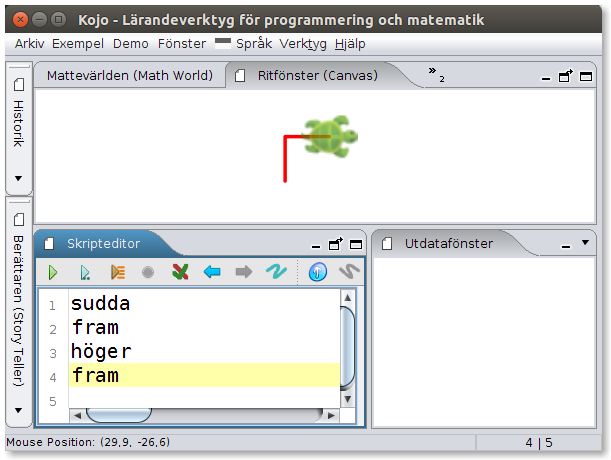
\includegraphics[width=0.7\textwidth]{../img/kojo}

\pause position, rikting, pennfärg, pennbredd, penna uppe/nere, fyllfärg
\end{Slide}




\begin{Slide}{Lata variabler och fördröjd evaluering}
Med nyckelordet \code{lazy} före \code{val} skapas en s.k. ''lat'' \Eng{lazy} variabel.
\begin{REPL}
scala> val striktVektor = Vector.fill(1000000)(math.random)
striktVektor: scala.collection.immutable.Vector[Double] =
 Vector(0.7583305221813246, 0.9016192590993339, 0.770022134260162, 0.15667718184929746, ...

scala> lazy val latVektor = Vector.fill(1000000)(math.random)
latVektor: scala.collection.immutable.Vector[Double] = <lazy>

scala> latVektor
res0: scala.collection.immutable.Vector[Double] =
  Vector(0.5391685014341797, 0.14759775960530275, 0.722606095900537, 0.9025572787055386, ...
\end{REPL}

En \code {lazy val} initialiseras \Alert{inte} vid deklarationen utan när den \Alert{refereras första gången}. Yttrycket som anges i deklarationen evalueras med s.k. \Emph{fördröjd evaluering} (även ''lat'' evaluering).
\end{Slide}

\begin{Slide}{Vad är egentligen skillnaden mellan \texttt{val}, \texttt{var}, \texttt{def} och \texttt{lazy val}?}
\begin{Code}[basicstyle=\ttfamily\fontsize{8}{11}\selectfont]
object slump {
  val förAlltidSammaReferens  = math.random
  var kanÄndrasMedTilldelning = math.random
  def evaluerasVidVarjeAnrop  = math.random
  lazy val fördröjdInit       = Vector.fill(1000000)(math.random)
}
\end{Code}
\vspace{1em}\pause
Lat evaluering är en viktig princip inom funktionsprogrammering som möjliggör effektiva, oföränderliga datastrukturer där element allokeras först när de behövs. \\
\href{https://en.wikipedia.org/wiki/Lazy_evaluation}{en.wikipedia.org/wiki/Lazy\_evaluation}
\end{Slide}





\Subsection{Funktioner är objekt}

\begin{Slide}{Programmeringsparadigm}
\href{https://en.wikipedia.org/wiki/Programming_paradigm}{en.wikipedia.org/wiki/Programming\_paradigm}:
\begin{itemize}
\item \Emph{Imperativ programmering}: programmet är uppbyggt av sekvenser av olika satser som läser och \Alert{ändrar} tillstånd
\item \Emph{Objektorienterad programmering}: en sorts imperativ programmering där programmet består av objekt som kapslar in tillstånd och erbjuder operationer som läser och \Alert{ändrar} tillstånd.
\item \Emph{Funktionsprogrammering}: programmet är uppbyggt av samverkande (matematiska) funktioner som \Alert{undviker} föränderlig data och tillståndsändringar. Oföränderliga datastrukturer skapar effektiva program i kombination med lat evaluering och rekursion.
\end{itemize}
\end{Slide}


\begin{Slide}{Funktioner är äkta objekt i Scala}
Scala visar hur man kan \Alert{förena} \Eng{unify} \\ \Emph{objekt-orientering} och \Emph{funktionsprogrammering}: \\\vspace{0.5em}

\textbf{\Large En funktion är ett objekt av funktionstyp\\ som har en \code{apply}-metod.}
\pause
\begin{REPLnonum}
scala> object öka extends (Int => Int) {
         def apply(x: Int) = x + 1
       }


scala> öka(1)
res0: Int = 2

scala> öka.   // tryck TAB
andThen   apply   compose   toString
\end{REPLnonum}
Mer om \code{extends} senare i kursen... %extends (Int => Int skrivs om till Function1[Int, Int]
\end{Slide}



\Subsection{SimpleWindow}
\begin{Slide}{Färdiga, enkla funktioner för att rita finns i klassen \texttt{cslib.window.SimpleWindow}}
På labben ska du använda \code{cslib.window.SimpleWindow}
\begin{itemize}
\item Paketet \code{cslib} innehåller paketet \code{window} som innehåller Java-klassen \code{SimpleWindow}.
%\item En \Emph{klass} är en ''mall'' för att göra \Emph{objekt}.
\item Med \code{SimpleWindow} kan man skapa ritfönster.
%\item När man skapar ett objekt från en klass använder man nyckelordet \code{new}.
\item Ladda ner \url{http://cs.lth.se/pgk/cslib} och lägg sedan jar-filen den katalog där du startar REPL med: \code{scala -cp cslib.jar}
\end{itemize}
\pause
\begin{REPLnonum}
$ scala -cp cslib.jar
scala> val w = new SimpleWindow(200,200,"hejsan")
\end{REPLnonum}
\pause Studera dokumentationen för \code{cslib.window.SimpleWindow} här: \url{http://cs.lth.se/pgk/api/}
\end{Slide}


\ifkompendium\else


\Subsection{Veckans övning och laboration}

\begin{Slide}{Övning \texttt{functions}}\SlideFontTiny
\setlength{\leftmargini}{0pt}
\begin{itemize}
%!TEX encoding = UTF-8 Unicode
%!TEX root = ../exercises.tex

\item Kunna skapa och använda funktioner med en eller flera parametrar, default-argument, och namngivna argument.
\item Kunna förklara nästlade funktionsanrop med aktiveringsposter på stacken.
\item Kunna förklara skillnaden mellan äkta och ''oäkta'' funktioner.
\item Kunna applicera en funktion på alla element i en samling.

\item Kunna använda funktioner som äkta värden.
\item Kunna skapa och använda anonyma funktioner (ä.k. lambda-funktioner).

\item Känna till att funktioner kan ha uppdelad parameterlista.
\item Känna till att det går att partiellt applicera argument på funktioner med uppdelad parameterlista för att skapa s.k. stegade funktioner (ä.k. curry-funktioner).

\item Känna till rekursion och kunna beskriva vad som kännetecknar en rekursiv funktion.
%\item Känna till att man kan loopa med rekursion och att svansrekursiva funktioner kan optimeras till while-loopar.

\item Känna till att det går att skapa egna kontrollstrukturer med hjälp av namnanrop.
\item Känna till skillnaden mellan värdeanrop och namnanrop.
\item Kunna tolka en stack trace.

\end{itemize}
\end{Slide}

\begin{Slide}{Lab \texttt{blockmole}}%\SlideFontTiny
%\setlength{\leftmargini}{0pt}
\begin{itemize}
%!TEX encoding = UTF-8 Unicode
%!TEX root = ../compendium2.tex

%\item Kunna kompilera Scalaprogram med \texttt{scalac}.
%\item Kunna köra Scalaprogram med \texttt{scala}.
%\item Kunna definiera och anropa funktioner.
%\item Kunna använda och förstå default-argument.
%\item Kunna ange argument med parameternamn.
\item Kunna skapa ett större program med din egen kod efter dina egna idéer.
\item Kunna använda en editor och terminalen för att iterativt editera, kompilera, och testa din kod.
\item Kunna använda variabler i kombination med alternativ och repetetition i flera nivåer.
\item Kunna stegvis förbättra din kod för att underlätta förändring och öka läsbarhet.
\item Kunna skapa och använda abstraktioner för att generalisera och möjliggöra återanvändning av kod.

\end{itemize}

\end{Slide}
\fi


\Lecture{5}{Klasser}
%!TEX encoding = UTF-8 Unicode
%!TEX root = ../lect-w05.tex

%%%

%TODO:
%  \begin{itemize}
%  \item Bygg upp \code{case class Complex(re: Double, im: Double)} steg för steg inspirerat av Pins3ed kap 6 i likhet med hur de gör med Rational
%  \item Illustrera följande begrepp: this (behövs i max(that)), method overloading behövs för att plussa med både Complex och Double
%  \item Till fördjupningsövning: dekorera Double med metoderna im och re samt (Double, Double) med metoden ir (för irrational) med implicit klass
%  \item Till extrauppgift: implementera klassen Polar(r, fi) med polära koordinater \url{https://sv.wikipedia.org/wiki/Pol%C3%A4ra_koordinater}
%  \end{itemize}

\Subsection{Vad är en klass?}

\ifkompendium
Begreppet \Emph{klass} är en viktig abstraktionsmekanism inom \Emph{objekt-orienterad programmering} (OOP). Klasser används för att samla funktioner och data. En klass har ett namn och kan ha parametrar. En klass deklareras med nyckelordet \code{class} och är en beskrivning hur en viss typ av objekt ska utformas när de så småningom skapas. Det går att skapa \Alert{många} objekt ur en och samma klass. 
\fi


\begin{Slide}{En metafor för klass: Stämpel}\SlideFontSmall
\begin{multicols}{2}

En klass liknar en \Emph{stämpel}.

\vspace{1em}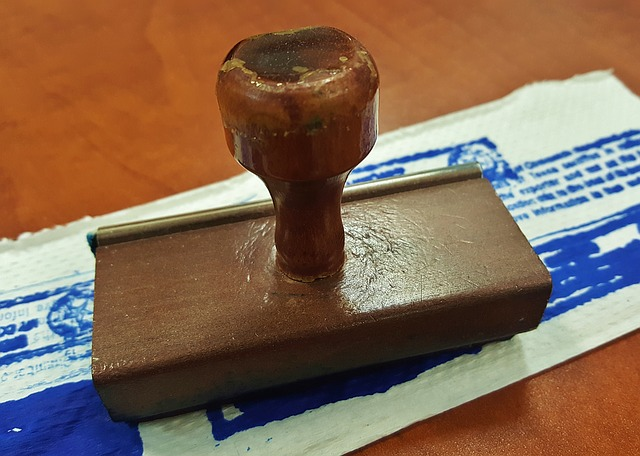
\includegraphics[width=0.5\textwidth]{../img/stamp}

\columnbreak

\pause

\begin{itemize}
\item En stämpel kan \Alert{tillverkas} -- motsvarar \Emph{deklaration} av klassen.
 \item Det händer inget förrän man \Alert{stämplar} -- motsvarar \Emph{instansiering}.
\item Då skapas \Alert{avbildningar} av stämpeln -- motsvarar \Emph{allokering av ett objekt} som är en \Emph{instans} av klassen.
\item Allokering kallas också \Emph{konstruktion} och funktionen/koden som gör själva allokeringen kallas \Emph{konstruktor}.
\end{itemize}

\end{multicols}
\end{Slide}


\begin{Slide}{Vad är en klass?}
\begin{itemize}
\item En klass är en mall \Eng{template} för att skapa objekt.
\item Objekt kan skapas med \code{new Klassnamn}, vilket kallas \Emph{instansiering}. 
\item I Scala 3 är \code{new} valfritt, det räcker med \code{Klassnamn()}. 
\item Ett objekt som skapats med en klassen \code{Klassnamn} som mall kallas för en \Emph{instans} av klassen \code{Klassnamn}.
\item En klass innehåller \Emph{medlemmar} \Eng{members}, som bl.a. kan vara:
  \begin{itemize}
  \item \Emph{attribut}, kallas även fält \Eng{field}: \code{val}, \code{lazy val}, \code{var}
  \item \Emph{metoder}, kallas även operationer: \code{def}
  \end{itemize}
\item Varje instans har sin uppsättning värden på attributen
vilka tillsammans utgör instansens \Emph{tillstånd}.
\end{itemize}

\end{Slide}
  


% \begin{Slide}[t]{Klass och instans}
% \vspace{-0.65em}
% \begin{REPLnonum}
% scala> class C { var attr = 42 }
%
% scala> val objRef1 = new C
% \end{REPLnonum}
% \vspace{3.7em}
% \begin{tikzpicture}[font=\SlideFontSmall\sffamily]
% \matrix [matrix of nodes, row sep=0, column 2/.style={nodes={rectangle,draw,minimum width=0.8cm}}] (mat)
% {
% \texttt{objRef1}   &  \makebox(10,10){ }\\
% };
%
% \node[cloud, cloud puffs=15.0, cloud ignores aspect, minimum width=2cm, minimum height=2cm,
%  align=center, draw] (instance1) at (3.8cm, 0.0cm) {
%  \begin{tabular}{r l}
%  \texttt{attr} & \fbox{42} \\
%  \end{tabular}
%  };
%
%
% \filldraw[black] ($ (mat-1-2) + (0.0cm,0.0cm) $) circle (3pt) node[] (ref1)  {};
% \draw [arrow, line width=0.7mm] (ref1) -- (instance1);
% \end{tikzpicture}
% \end{Slide}
%
%
%
% \begin{Slide}[t]{Klass och instans}
% \vspace{-0.5em}
% \begin{REPLnonum}
% scala> class C { var attr = 42 }
%
% scala> val objRef1 = new C
%
% scala> val objRef2 = new C
% \end{REPLnonum}
% \vspace{2em}
% \begin{tikzpicture}[font=\SlideFontSmall\sffamily]
% \matrix [matrix of nodes, row sep=0, column 2/.style={nodes={rectangle,draw,minimum width=0.8cm}}] (mat)
% {
% \texttt{objRef1}   &  \makebox(10,10){ }\\
% \texttt{objRef2}   &  \makebox(10,10){ }\\
% };
%
% \node[cloud, cloud puffs=15.0, cloud ignores aspect, minimum width=2cm, minimum height=2cm,
%  align=center, draw] (instance1) at (3.8cm, 0.35cm) {
%  \begin{tabular}{r l}
%  \texttt{attr} & \fbox{42} \\
%  \end{tabular}
%  };
%
% \node[cloud, cloud puffs=15.0, cloud ignores aspect, minimum width=2cm, minimum height=2cm,
%  align=center, draw] (instance2) at (5.8cm, -1.5cm) {
%  \begin{tabular}{r l}
%  \texttt{attr} & \fbox{42} \\
%  \end{tabular}
%  };
%
% \filldraw[black] ($ (mat-1-2) + (0.0cm,0.0cm) $) circle (3pt) node[] (ref1)  {};
% \draw [arrow, line width=0.7mm] (ref1) -- (instance1);
%
% \filldraw[black] ($ (mat-2-2) + (0.0cm,0.0cm) $) circle (3pt) node[] (ref2)  {};
% \draw [arrow, line width=0.7mm] (ref2) -- (instance2);
% \end{tikzpicture}
% \end{Slide}
%
%
%
% \begin{Slide}[t]{Klass och instans}
% \vspace{-0.5em}
% \begin{REPLnonum}
% scala> class C { var attr = 42 }
%
% scala> val objRef1 = new C
%
% scala> val objRef2 = new C
%
% scala> objRef2.attr = 43
% \end{REPLnonum}
% \begin{tikzpicture}[font=\SlideFontSmall\sffamily]
% \matrix [matrix of nodes, row sep=0, column 2/.style={nodes={rectangle,draw,minimum width=0.8cm}}] (mat)
% {
% \texttt{objRef1}   &  \makebox(10,10){ }\\
% \texttt{objRef2}   &  \makebox(10,10){ }\\
% };
%
% \node[cloud, cloud puffs=15.0, cloud ignores aspect, minimum width=2cm, minimum height=2cm,
%  align=center, draw] (instance1) at (3.8cm, 0.35cm) {
%  \begin{tabular}{r l}
%  \texttt{attr} & \fbox{42} \\
%  \end{tabular}
%  };
%
% \node[cloud, cloud puffs=15.0, cloud ignores aspect, minimum width=2cm, minimum height=2cm,
%  align=center, draw] (instance2) at (5.8cm, -1.5cm) {
%  \begin{tabular}{r l}
%  \texttt{attr} & \fbox{43} \\
%  \end{tabular}
%  };
%
%
% \filldraw[black] ($ (mat-1-2) + (0.0cm,0.0cm) $) circle (3pt) node[] (ref1)  {};
% \draw [arrow, line width=0.7mm] (ref1) -- (instance1);
%
% \filldraw[black] ($ (mat-2-2) + (0.0cm,0.0cm) $) circle (3pt) node[] (ref2)  {};
% \draw [arrow, line width=0.7mm] (ref2) -- (instance2);
% \end{tikzpicture}
% \end{Slide}



\begin{Slide}{Singelobjekt jämfört med klass}\SlideFontSmall
Vi har tidigare deklarerat \Emph{singelobjekt} som bara finns i \Alert{en} enda upplaga:
\begin{REPLnonum}
scala> object Björn { var ålder = 53; val längd = 178 }
\end{REPLnonum}

Med en \Emph{klass} kan man skapa \Alert{godtyckligt många} \Emph{instanser av klassen} med hjälp av nyckelordet \code{new} följt av klassens namn:

\begin{REPLnonum}
scala> class Person { var ålder = 0; var längd = 0 }

scala> val björn = new Person   // allokera plats i minnet
björn: Person = Person@7ae75ba6  // unikt id för instansen
\end{REPLnonum}
\begin{tikzpicture}[font=\small\sffamily]
\matrix [matrix of nodes, row sep=0, column 2/.style={nodes={rectangle,draw,minimum width=0.8cm}}] (mat)
{
\texttt{björn}   &  \makebox(10,10){ }\\
};
\node[cloud, cloud puffs=12.0, cloud ignores aspect, minimum width=2cm, minimum height=3.8cm,
 align=center, scale=0.8, draw] (x) at (3.8cm, -1.0cm) {
 \begin{tabular}{r l}
 \multicolumn{2}{c}{\ttfamily\itshape Person@7ae75ba6}\\ \\
 \texttt{ålder} & \fbox{~0~} \\
 \texttt{längd} & \fbox{~0~}\\
 \end{tabular}
 };
\filldraw[black] (0.6cm,0.0cm) circle (3pt) node[] (ref) {};
\draw [arrow, line width=0.7mm] (ref) -- (x);
\end{tikzpicture}
\end{Slide}


\begin{Slide}{Förändring av objektets tillstånd}
\begin{REPLnonum}
scala> björn.ålder = 53

scala> björn.längd = 178
björn: Person = Person@7ae75ba6
\end{REPLnonum}

\begin{tikzpicture}[font=\large\sffamily]
\matrix [matrix of nodes, row sep=0, column 2/.style={nodes={rectangle,draw,minimum width=0.8cm}}] (mat)
{
\texttt{björn}   &  \makebox(10,10){ }\\
};
\node[cloud, cloud puffs=13.0, cloud ignores aspect, minimum width=2cm, minimum height=3.8cm,
 align=center, draw] (x) at (5.8cm, -1.2cm) {
 \begin{tabular}{r l}
 \multicolumn{2}{c}{\ttfamily\itshape Person@7ae75ba6}\\ \\
 \texttt{ålder} & \fbox{~53~} \\
 \texttt{längd} & \fbox{~178~}\\
 \end{tabular}
 };
\filldraw[black] (0.75cm,0.0cm) circle (3pt) node[] (ref) {};
\draw [arrow, line width=0.7mm] (ref) -- (x);
\end{tikzpicture}
%{\SlideFontTiny{\ttfamily\itshape Person@7ae75ba6} är en unik idenfierare för instansen, så att JVM hittar den i heapen.}
\end{Slide}


\begin{Slide}{Bättre att initialisera med hjälp av klassparametrar}
\begin{REPLnonum}
scala> class Person(var ålder: Int, var längd: Int)

scala> val sandra = new Person(42, 166)
sandra: Person = Person@7878bbdb
\end{REPLnonum}

\begin{tikzpicture}[font=\large\sffamily]
\matrix [matrix of nodes, row sep=0, column 2/.style={nodes={rectangle,draw,minimum width=0.8cm}}] (mat)
{
\texttt{sandra}   &  \makebox(10,10){ }\\
};
\node[cloud, cloud puffs=13.0, cloud ignores aspect, minimum width=2cm, minimum height=3.8cm,
 align=center, draw] (x) at (5.8cm, -1.2cm) {
 \begin{tabular}{r l}
 \multicolumn{2}{c}{\ttfamily\itshape Person@7878bbdb}\\ \\
 \texttt{ålder} & \fbox{~42~} \\
 \texttt{längd} & \fbox{~166~}\\
 \end{tabular}
 };
\filldraw[black] (0.75cm,0.0cm) circle (3pt) node[] (ref) {};
\draw [arrow, line width=0.7mm] (ref) -- (x);
\end{tikzpicture}
%{\SlideFontTiny{\ttfamily\itshape Person@7ae75ba6} är en unik idenfierare för instansen, så att JVM hittar den i heapen.}
\end{Slide}


\begin{Slide}{Klassdeklarationer och instansiering}\SlideFontSmall
\setlength{\leftmargini}{0pt}
\begin{itemize}
\item Syntax för deklaration av klass: \\ \vspace{0.5em}{\SlideFontSize{13}{16}\code|class Klassnamn(parametrar){ medlemmar }|}\vspace{0.5em}
\item Exempel: \Emph{deklaration}
\begin{Code}
class Klassnamn(val attribut1: Int, attribut2: String){
  val attribut3: Double = 42.0              //publikt oföränderligt attribut
  private var attribut4: Boolean = false    //privat medlem syns inte utåt
  def metod(parameter: Int) = parameter + 1 //funktion i klass kallas metod
  lazy val attr5 = Vector.fill(100000)(42.0)     //fördröjd initialisering
}
\end{Code}

\item Parametrar initialiseras med de argument som ges vid \code{new}.
\item Exempel: \Emph{instansiering} med argument för initialisering av klassparametrar
\begin{Code}
val instansReferens = new Klassnamn(42, "hej")  // new är valfritt här 
\end{Code}

\item Parametrar som inte föregås av modifierare (t.ex. private val, val, var) blir \Emph{attribut} som är \code{ private[this] val } och bara är synliga i \Alert{denna} instans.
\item Attribut i klasskroppen är \Emph{publika} (alltså synliga utåt) om inte \code{private} anges.
\end{itemize}
\end{Slide}




\begin{Slide}{Övning: en klass som representerar en person}
\begin{enumerate}
  \item Deklarera en klass \code{Person} med dessa publika attribut:
  \begin{itemize}
    \item oföränderligt förnamn
    \item oföränderligt efternamn
    \item förändringsbar ålder med defaultargument \code{0}
  \end{itemize}
  \item lägg till en metod i klasskroppen med explicit returtyp som ger en 2-tupel med förnamn och efternamn
  \item skriv en deklaration som deklarerar en variabel \code{p} som initialiseras med värdet av ett uttryck som instansierar klassen \code{Person} med ditt namn och din ålder som nyfödd.
  \item skriv en sats som skriver ut ditt förnamn genom att referera attribut med punktnotation
  \item skriv en tilldelningssats som ändrar tillståndet för den instans som referensen \code{p} refererar till så att åldersattributets värde blir din nuvarande ålder
\end{enumerate}
\end{Slide}



\begin{Slide}{Lösning: klassen Person}
\begin{Code}[basicstyle=\SlideFontSize{6.9}{9}\ttfamily]
class Person(val givenName: String, val familyName: String, var age: Int = 0){
  def name: (String, String) = (givenName, familyName)
}
\end{Code}
\begin{REPLnonum}[basicstyle=\SlideFontSize{7}{9}\ttfamily\color{white}]
val p = Person("Björn", "Regnell")
println(p.name._1)
p.age = 50
\end{REPLnonum}
\end{Slide}


\begin{Slide}{Instansprivata klassparametrar}\SlideFontSmall
\setlength{\leftmargini}{0pt}

\begin{itemize}
\item Parametrar som inte föregås av modifierare (t.ex. private val, val, var) blir \Emph{attribut} som är \code{ private[this] val } och bara är synliga i \Alert{denna} instans.
\item Exempel på konsekvensen av \code{private[this]}:
\begin{REPL}[basicstyle=\SlideFontSize{6.7}{9}\ttfamily\color{white}]
scala> class C(a: Int){ def add(other: C): Int = a + other.a }
error: value a is not a member of C

// betyder samma sak som:

scala> class C(private[this] val a: Int){ def add(other: C): Int = a + other.a }
error: value a is not a member of C
\end{REPL}
\item Men detta fungerar fint:
\begin{REPL}
scala> class D(val a: Int){ def add(other: D): Int = a + other.a }

scala> D(42).add(D(43))
res0: Int = 85
\end{REPL}
...eftersom modifieraren \code{val} framför klassparameter ger publik synlighet.
\item Vad händer om du skriver \code{private val} framför klassparametern \code{a} ovan?
\end{itemize}
\end{Slide}


\begin{Slide}{\texttt{private} jämfört med \texttt{private[this]}}\SlideFontSmall
\code{private[this]} är \Alert{ännu} mer privat än \code{private}
\begin{Code}
class Hemlis(private val hemlis: Int) {
  def ärSammaSom(annan: Hemlis) = hemlis == annan.hemlis   // Funkar!
}

class Hemligare(private[this] val hemlis: Int) {
  def ärSammaSom(annan: Hemligare) = hemlis == annan.hemlis //KOMPILERINGSFEL
}
\end{Code}
\pause Vad händer om man inte skriver ens \code{val}? \pause Olika för klass och s.k. case-klass:
\begin{Code}
class Hemligare(hemlis: Int) { // motsvarar private[this] val
  def ärSammaSom(annan: Hemligare) = hemlis == annan.hemlis //KOMPILERINGSFEL
}

case class InteHemlig(seMenInteRöra: Int) { // blir automatiskt val
  def ärSammaSom(annan: InteHemlig): Boolean =
    seMenInteRöra == annan.seMenInteRöra
}

\end{Code}
{\SlideFontTiny Vi ska lära mer om det godis man får på köpet med \code{case}-klasser om ett litet tag.}
\end{Slide}



%%%%%%%%%%%% ÄR EXEMPEL KOMPLEXA TAL ÄR FÖR SVÅR MATEMATIK för lp1???? %%%%%%%%%
%% Nej komplexa tal som vektor med polära koordinater ingår i matte 4 som är krav för LTH: %%%


\begin{Slide}{Övning: Klassen Complex i Scala}\SlideFontSmall
Implementera klassen \code{Complex} nedan som representerar komplexa tal:
\begin{Code}
  class Complex(val re: Double, val im: Double):
    def r  = ???  // absolutbeloppet
    def fi = ???  // vinkeln i radianer
    def +(other: Complex): Complex = ???  // resultatet av addition
    var imSymbol = 'i'  // symbol för imaginärdel, används i toString
    override def toString = ???  // en strängrepresentation av talet
\end{Code}

\begin{minipage}{0.3\textwidth}
  Exempel: \\$z = 3 + 4i$
\end{minipage}
\begin{minipage}{0.5\textwidth}
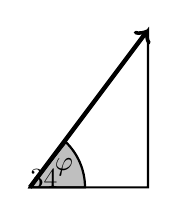
\begin{tikzpicture}[thick]
\coordinate (O) at (0,0);
\coordinate (A) at (1.5,0);
\coordinate (B) at (1.5,2.0);

%\tkzMarkAngle[fill=orange,size=0.5cm, opacity=.4](A,O,B) 
%\tkzLabelAngle[pos=0.8](A,O,B){\texttt{$\varphi$}}
 %%% AAAARGH ovan slutade funka så gjorde nedan HACK i stället
\draw[fill=lightgray, thick] (0,0) -- (0:0.7cm) arc (0:46:0.8cm) node at (30:0.5cm) {$\varphi$} -- cycle;
%\draw[fill=lightgray, thick] (0,0) -- (0:0.7cm) arc (0:45:0.8cm) node at (30:0.5cm) {$\varphi$} -- cycle;
%https://tex.stackexchange.com/questions/96459/automatically-draw-and-labels-angles-of-a-triangle-in-tikz

\draw (O)--(A)--(B)--cycle;
\draw [->, ultra thick] (O)--(B);

\tkzLabelSegment[below=5pt](O,A){\textit{real-delen} är $3$}
\tkzLabelSegment[above left=5pt](O,B){\textit{r}}
\tkzLabelSegment[right=5pt](A,B){\textit{imaginär-delen} är $4$}


\end{tikzpicture}
\end{minipage}

\end{Slide}


\begin{Slide}{Exempel: Klassen Complex i Scala}\SlideFontSmall
\scalainputlisting[basicstyle=\ttfamily\SlideFontSize{7}{9}]{../compendium/examples/complex1.scala}
%Klassparametrarna är parametrar till den s.k. \Emph{primärkonstruktorn}.
\begin{REPL}
scala> val z = new Complex(3, 4)  // konstruktion av instans av Complex
z: Complex = 3.0 + 4.0i

scala> val polärForm = (c1.r, c1.fi)
polärForm: (Double, Double) = (5.0,0.6435011087932844)

scala> val z2 = new Complex(1, 2)
z2: Complex = 1.0 + 2.0i

scala> z1 + z2
res0: Complex = 4.0 + 6.0i
\end{REPL}
\end{Slide}



\begin{Slide}{Exempel: Principen om enhetlig access}\SlideFontSmall
\scalainputlisting[basicstyle=\ttfamily\SlideFontSize{7}{9}]{../compendium/examples/complex2.scala}
\pause
\begin{itemize}
\item Efter som attributen \code{re} och \code{im} är oföränderliga, kan vi lika gärna ändra i klass-implementationen och göra om metoderna \code{r} och \code{fi} till \code{val}-variabler utan att klientkoden påverkas.

\item Då anropas \code{math.hypot} och \code{math.atan2} bara en gång vid initialisering (och inte varje gång som med \code{def}).

\item Vi skulle även kunna använda \code{lazy val} och då bara räkna ut \code{r} och \code{fi} om och när de verkligen refereras av klientkoden, annars inte.

\item Eftersom klientkoden inte ser skillnad på metoder och variabler, kallas detta \Emph{principen om enhetlig access}. (Många andra språk har \Alert{inte} denna möjlighet, tex Java där metoder \emph{måste} ha parenteser.)
\end{itemize}
\end{Slide}



\Subsection{Olika sätt att skapa instanser}

\begin{Slide}{Instansiering med direkt användning av \texttt{new}}

Instansiering genom \Emph{direkt användning} av \code{new}\\
{\SlideFontSmall (här första varianten av Complex med \code{r} och \code{fi} som metoder)}
\begin{REPLnonum}
scala> val c1 = new Complex(3, 4)
\end{REPLnonum}
\begin{tikzpicture}[font=\SlideFontSmall\sffamily]
\matrix [matrix of nodes, row sep=0, column 2/.style={nodes={rectangle,draw,minimum width=0.8cm}}] (mat)
{
\texttt{c1}   &  \makebox(10,10){ }\\
};

\node[cloud, cloud puffs=15.0, cloud ignores aspect, minimum width=2cm, minimum height=3.8cm,
 align=center, draw] (instance1) at (5.8cm, -1.5cm) {
 \begin{tabular}{r l l}
 \texttt{re:} & \texttt{Double} & \fbox{3.0} \\
 \texttt{im:} & \texttt{Double} & \fbox{4.0}\\
 \texttt{imSymbol:} & \texttt{Char} & \fbox{i}\\
 \end{tabular}
 };

\filldraw[black] ($ (mat-1-2) + (0.0cm,0.0cm) $) circle (3pt) node[] (ref1)  {};

\draw [arrow, line width=0.7mm] (ref1) -- (instance1);
\end{tikzpicture}
\pause
Ofta vill man göra \Alert{indirekt} instansiering så att vi senare har friheten att ändra hur instansiering sker.
\end{Slide}



\begin{Slide}{Indirekt instansiering med fabriksmetoder}\SlideFontSmall
En \Emph{fabriksmetod} är en metod som används för att instansiera objekt.
\begin{Code}[basicstyle=\SlideFontSize{8}{12}\ttfamily\selectfont]
object MyFactory {
  def createComplex(re: Double, im: Double) = new Complex(re, im)
  def createReal(re: Double)                = new Complex(re, 0)
  def createImaginary(im: Double)           = new Complex(0, im)
}
\end{Code}
\pause
Instansiera \Alert{inte direkt}, utan \Emph{indirekt} genom användning av \Emph{fabriksmetoder}:
\begin{REPL}
scala> import MyFactory._

scala> createComplex(3, 4)
res0: Complex = 3.0 + 4.0i

scala> createReal(42)
res1: Complex = 42.0 + 0.0i

scala> createImaginary(-1)
res2: Complex = 0.0 + -1.0i
\end{REPL}
\end{Slide}



\begin{Slide}{Hur förhindra direkt instansiering?}
Om vi vill \Emph{förhindra direkt instansiering} kan vi göra primärkonstruktorn \Alert{privat}:
\scalainputlisting[basicstyle=\ttfamily\SlideFontSize{7}{9}]{../compendium/examples/complex3.scala}
MEN... då går det ju \Alert{inte} längre att instansiera något alls!  \code{   :(}
\begin{REPLnonum}
scala> new Complex(3,4)
error:
 constructor Complex in class Complex cannot be accessed
\end{REPLnonum}
\end{Slide}



\begin{Slide}{Kompanjonsobjekt med indirekt instansiering}\SlideFontSmall
\setlength{\leftmargini}{0pt}
\begin{itemize}
\item Ett \Emph{kompanjonsobjekt} \Eng{companion object} är ett singelobjekt som ligger i \Alert{samma kodfil} som en klass, och som har \Alert{samma namn} som klassen.

\item Medlemmar i ett kompanjonsobjekt \Alert{får accessa privata} medlemmar i kompanjonsklassen (och vice versa) och kompanjonsobjektet får därför accessa privat konstruktor och kan göra \code{new}.
\scalainputlisting[basicstyle=\ttfamily\SlideFontSize{7}{9}]{../compendium/examples/complex4.scala}

\item Fabriksmetoder i kompanjonsobjektet ovan och privat konstruktor gör att vi \Alert{enbart} tillåter \Emph{indirekt instansiering}.
\end{itemize}
\end{Slide}

\begin{Slide}{Användning av kompanjonsobjekt med fabriksmetoder}
Nu kan vi \Alert{bara} instansiera \Emph{indirekt}!  \code{   :)}
\begin{REPLnonum}
scala> Complex.real(42.0)
res0: Complex = 42.0 + 0.0i

scala> Complex.imag(-1)
res1: Complex = 0.0 + -1.0i

scala> Complex.apply(3,4)
res2: Complex = 3.0 + 4.0i

scala> Complex(3,4)
res3: Complex = 3.0 + 4.0i

scala> new Complex(3, 4)
error:
     constructor Complex in class Complex cannot be accessed
\end{REPLnonum}
\end{Slide}


\begin{Slide}{Alternativa direktinstansieringar med default-argument}\SlideFontSmall
Med \Emph{default-argument} kan vi erbjuda \Emph{alternativa} sätt att direktinstansiera.
\scalainputlisting[basicstyle=\ttfamily\SlideFontSize{7}{9}]{../compendium/examples/complex5.scala}
\begin{REPL}
scala> new Complex()
res0: Complex = 0.0 + 0.0i

scala> new Complex(re = 42)  //anrop med namngivet argument
res1: Complex = 42.0 + 0.0i

scala> new Complex(im = -1)
res2: Complex = 0.0 + -1.0i

scala> new Complex(1)
res3: Complex = 1.0 + 0.0i
\end{REPL}
\end{Slide} 

\begin{Slide}{Alternativa sätt att instansiera med fabriksmetod}
Vi kan också erbjuda \Emph{alternativa} sätt att instansiera \Emph{indirekt} med fabriksmetoden \code{apply} i ett kompanjonsobjekt genom default-argument:
\scalainputlisting[basicstyle=\ttfamily\SlideFontSize{7}{9}]{../compendium/examples/complex6.scala}

\end{Slide}

\begin{Slide}{Medlemmar som bara behövs i en enda upplaga}
Attributet \code{imSymbol} passar bättre att ha i \Emph{kompanjonsobjektet}, eftersom det räcker att ha \Alert{en enda upplaga}, som kan vara gemensam för alla objekt:
\scalainputlisting[basicstyle=\ttfamily\SlideFontSize{7}{9}]{../compendium/examples/complex7.scala}

\end{Slide}



\begin{Slide}{Medlemmar i singelobjekt är statiskt allokerade}\SlideFontTiny

Minnesplatsen för \Emph{attribut i singelobjekt} allokeras automatiskt en gång för alla, och kallas därför \Emph{statiskt} allokerad. Singelobjektets namn \code{Complex} utgör en statisk referens till den enda instansen och är av typen \texttt{Complex.type}.

\begin{tikzpicture}[font=\SlideFontSmall\sffamily]
\matrix [matrix of nodes, row sep=0, column 2/.style={nodes={rectangle,draw,minimum width=0.8cm}}] (mat)
{
\texttt{Complex}   &  \makebox(10,10){ }\\
};

\node[cloud, cloud puffs=15.0, cloud ignores aspect, minimum width=1cm, minimum height=2cm,
 align=center, draw] (instance1) at (5.8cm, 0.0cm) {
 \begin{tabular}{r l l}
 \texttt{imSymbol:} & \texttt{Char} & \fbox{i}\\
 \end{tabular}
 };

\filldraw[black] ($ (mat-1-2) + (0.0cm,0.0cm) $) circle (3pt) node[] (ref1)  {};

\draw [arrow, line width=0.7mm] (ref1) -- (instance1);
\end{tikzpicture}

Nu bereder vi inte plats för \code{imSymbol} i varenda \Emph{dynamiskt} allokerade instans:
\begin{REPLnonum}
scala> val c1 = Complex(3, 4)
\end{REPLnonum}

\begin{tikzpicture}[font=\SlideFontSmall\sffamily]
\matrix [matrix of nodes, row sep=0, column 2/.style={nodes={rectangle,draw,minimum width=0.8cm}}] (mat)
{
\texttt{c1}   &  \makebox(10,10){ }\\
};

\node[cloud, cloud puffs=15.0, cloud ignores aspect, minimum width=2cm, minimum height=2cm,
 align=center, draw] (instance1) at (5.8cm, -0.0cm) {
 \begin{tabular}{r l l}
 \texttt{re:} & \texttt{Double} & \fbox{3.0} \\
 \texttt{im:} & \texttt{Double} & \fbox{4.0}\\
 \end{tabular}
 };

\filldraw[black] ($ (mat-1-2) + (0.0cm,0.0cm) $) circle (3pt) node[] (ref1)  {};

\draw [arrow, line width=0.7mm] (ref1) -- (instance1);
\end{tikzpicture}


\end{Slide}




\begin{Slide}{Attribut i kompanjonsobjekt användas för sådant som är gemensamt för alla instanser}

Om vi ändrar på statiska \code{imSymbol} så ändras \code{toString} för \Alert{alla} dynamiskt allokerade instanser.
\begin{REPLnonum}
scala> val c1 = Complex(3, 4)
c1: Complex = 3.0 + 4.0i

scala> Complex.imSymbol = 'j'
Complex.imSymbol: Char = j

scala> val c2 = Complex(5, 6)
c2: Complex = 5.0 + 6.0j

scala> c1
res0: Complex = 3.0 + 4.0j
\end{REPLnonum}
\end{Slide}


\Subsection{Case-klasser och fördelen med oföränderlighet}

\ifkompendium\else
\begin{frame}[plain]
  
\includegraphics[width=1.0\textwidth]{../img/mutant.png}
\end{frame}
\fi

\begin{Slide}{Övning: en läskig mutant}\SlideFontSmall
\begin{enumerate}
\item Skapa en klass med namnet \code{Mutant} som har ett förändringsbart attribut som klassparameter med namnet \code{i} av typen \code{Int} med default-argumentet \code{5}.
\vspace{0.5em}

\item \begin{minipage}{0.5\textwidth}
Deklarera två \code{val}-variabler som kallas \code{fem1} och \code{fem2} och som båda refererar till \Alert{samma} \code{Mutant}-instans.
\end{minipage}
\hfill\begin{minipage}{0.32\textwidth}
\hfill
\includegraphics[width=3.4cm]{../img/mutant.png}

En \code{Mutant}-instans där \code{i} kanske är fem.
\vspace{1em}
\end{minipage}

\item Skriv kod som ändrar tillstånd via den ena mutantreferensen.

\item Syns ändringen via den andra mutantreferensen?
\end{enumerate}
\end{Slide}




\begin{Slide}{Case-klasser}
Case-klasser är ett smidigt sätt att skapa \Emph{oföränderliga} datastrukturer. Med nyckelordet \code{case} framför \code{class} får du mycket ''godis på köpet'':

\begin{itemize}
\item Klassparametrar blir automatiskt publika oföränderliga attribut\footnote{alltså \Alert{inte} \texttt{private[this] val } som i vanliga klasser.} och du slipper alltså skriva \code{val}
\item Du får en automatisk \Emph{toString} med klassens namn och värdet av alla \code{val}-attribut som ges av klassparametrarna och du slipper alltså skriva en egen toString
\item Du får ett automatiskt kompanjonsobjekt med en fabriksmetod \code{apply} för indirekt instansiering där alla klassparametrarnas \code{val}-attribut initialiseras.
\pause
\item ... och mer därtill men mer om det senare...
\end{itemize}
\end{Slide}




\begin{Slide}{Exempel: oföränderliga case-klassen \code{Point}}

\begin{Code}[basicstyle=\SlideFontSize{10}{12}\ttfamily]
case class Point(x: Double, y: Double)
\end{Code}

\begin{REPLnonum}
scala> val p1 = Point(3, 4)
p1: Point = Point(3.0,4.0)

scala> val p2 = p1
p2: Point = Point(3.0,4.0)

scala> p1.x = 42
error: reassignment to val
\end{REPLnonum}
Vi kan utan risk dela med oss av en referens till en oföränderlig klass -- ingen kan ändra dess innehåll. (Jämför läskiga mutanten i tidigare exempel.)

\end{Slide}






\Subsection{Konstruktor}



\begin{Slide}{Vad är en konstruktor?}
\begin{itemize}
\item En \Emph{konstruktor} är den maskinkod som exekveras när klasser instansieras med \code{new}.

\item Konstruktorn skapar ett nytt objekt i minnet vid varje anrop.

\item I Scala \Alert{genererar kompilatorn} en \Emph{primärkonstruktor} åt dig med maskinkod som initialiserar alla attribut baserat på klassparametrarna som du deklarerat.

\pause

%\item I Java och många andra språk får man \Alert{explicit} skriva kod för konstruktorer med speciell syntax och göra alla initialiseringar av attribut själv, och det behövs många olika konstruktorer för att motsvara defaultargument.

\item I Scala \Emph{kan} man också skriva egna alternativa s.k. \Emph{hjälpkonstruktorer}, men det är \Alert{ovanligt}, eftersom man har möjligheten med fabriksmetoder i kompanjonsobjekt och default-argument.
\end{itemize}
\end{Slide}


\begin{Slide}{Hjälpkonstruktorer i Scala (ovanliga)}%\SlideFontSmall
Fördjupning för kännedom:
\begin{itemize}
\item I Scala kan man skapa ett alternativ till primärkonstruktorn, en så kallad \Emph{hjälpkonstruktor} \Eng{auxilliary constructor} genom att deklarera en metod med det speciella namnet \code{this}.


\item Hjälpkonstruktorer \Alert{måste} börja med att anropa en \Alert{annan} konstruktor som står \Alert{före} i koden, till exempel primärkonstruktorn.
\end{itemize}

\begin{Code}
class Point(val x: Int, val y: Int, val z: Int): // primärkonstruktor
  def this(x: Int, y: Int) = this(x, y, 0) // anropa primärkonstruktorn
  def this(x: Int) = this(x, 0) // anropa hjälpkonstruktor
\end{Code}

%{\SlideFontSmall Överlagrade hjälpkonstruktorer i Scala liknar användning av konstruktorer i Java, där man inte har default-argument och apply i kompanjonsobj. etc.}

\end{Slide}

\begin{Slide}{Användning av hjälpkonstruktor}
\begin{REPL}
scala> val p1 = Point(1)
p1: Point = Point@21312342

scala> val p2 = Point(1, 2)
p2: Point = Point@43254325

scala> val p3 = Point(1, 2, 3)
p3: Point = Point@346654
\end{REPL}
\pause
Men man gör \Alert{mycket oftare} så här i Scala:
\begin{Code}[basicstyle=\ttfamily\SlideFontSize{8.5}{12}]
case class Point(x: Int, y: Int = 0, z: Int = 0)
\end{Code}
Använd alltså defaultargument hellre än hjälpkonstruktor.\\
(Eller överlagrad fabriksmetod i kompanjonsobjekt.)
\end{Slide}



% \begin{Slide}{Vad gör skräpsamlaren?}\SlideFontSmall
% \begin{itemize}
% \item Scala och Java är båda programmeringsspråk som förutsätter en körmiljö med \Alert{automatisk}  \Emph{skräpsamling} \Eng{garbage collection}.
%
% \item \Emph{Skräpsamlaren} \Eng{the garbage collector} är ett program som automatiskt körs i bakgrunden då och då och \Emph{städar minnet} genom att frigöra den plats som upptas av \Alert{objekt som inte längre används}.
%
% \item JVM:en bestämmer själv när skräpsamlaren ska jobba och programmeraren har ingen kontroll över detta.
%
% \item Den stora \Emph{fördelen} med automatisk skärpsamling är att man slipper bry sig om det svåra och felbenägna arbetet att \Alert{avallokera} minne.
%
% \item \Alert{Nackdelen} är att man inte kan styra exakt hur och när skräpsamlingen ska ske och man kan därmed inte bestämma när processorn ska belastas med minneshanteringen. Detta är normalt inget problem, utom i vissa tidskritiska realtidssystem med hårda minnesbegränsningar och svarstidskrav.
%
% \item I språk utan automatisk skräpsamling, t.ex. C++, måste man ta hand om destruktion av objekt och skriva egna s.k. \Emph{destruktorer}.
% \end{itemize}
% \end{Slide}


\Subsection{Referens saknas: \texttt{null}}

\begin{Slide}{Referens saknas: \texttt{null}}
\begin{itemize}
\item I Java och många andra språk använder man ofta literalen \code{null} för att representera att ett \Alert{värde saknas}.

\item En referens som är \code{null} refererar inte till någon instans.

\item Om du försöker referera till instansmedlemmar med punktnotation genom en referens som är \code{null} kastas ett \Alert{undantag} \code{NullPointerException}.

\item Oförsiktig användning av \code{null} är en vanlig källa till \Alert{buggar}, som kan vara svåra att hitta och fixa.

\end{itemize}
\end{Slide}


\begin{Slide}{Exempel: \texttt{null}}
\begin{REPL}
scala> class Gurka(val vikt: Int)

scala> var g: Gurka = null        // ingen instans allokerad än
val g: Gurka = null

scala> g.vikt
java.lang.NullPointerException

scala> g = Gurka(42)          // instansen allokeras
val g: Gurka = Gurka@1ec7d8b3

scala> g.vikt
val res0: Int = 42

scala> g = null         // instansen kommer att destrueras av skräpsamlaren
\end{REPL}

\begin{itemize} \SlideFontSmall
\item Scala har \code{null} av kompabilitetsskäl, men det är brukligt att \Alert{endast} använda \code{null} om man anropar Java-kod.

\item Scala erbjuder smidiga \code{Option}, \code{Some} och \code{None} för säker hantering av saknade värden; mer om detta kommande vecka.



\end{itemize}
\end{Slide}


\Subsection{Referensen \texttt{this}}
\begin{Slide}{Referensen \texttt{this}}\SlideFontSmall
\begin{itemize}
\item Nyckelordet \code{this} ger en referens till den aktuella instansen.
\begin{REPLnonum}
scala> class Gurka(var vikt: Int){def jagSjälv = this}

scala> val g = Gurka(42)
val g: Gurka = Gurka@5ae9a829

scala> g.jagSjälv
val res0: Gurka = Gurka@5ae9a829

scala> g.jagSjälv.vikt
val res1: Int = 42

scala> g.jagSjälv.jagSjälv.vikt
val res2: Int = 42
\end{REPLnonum}
\item Referensen \code{this} används ofta för att komma runt ''namnkrockar'' där variabler med samma namn gör så att den ena variabeln inte syns.
\end{itemize}
\end{Slide}



\Subsection{Getters och setters}

\begin{Slide}{Getters och setters}\SlideFontSmall
\begin{itemize}
\item I många språk (t.ex. Java, Python) finns inget motsvarande nyckelord \code{val} som garanterar oföränderliga attributreferenser.
\footnote{Java har visserligen \jcode{final} men det är annorlunda som vi ska se senare.}

\item Därför gör man i dessa språk nästan alltid alla attribut \Alert{privata} för att förhindra att de ändras på ett okontrollerat sätt.

% \item Många språk följer \Alert{inte} principen om enhetlig access: åtkomst av metoder och variabler sker med olika syntax.

\item Därför är det normalt att införa metoder som kallas \Emph{getters} och \Emph{setters}, som används för att \Alert{indirekt} läsa och uppdatera \Emph{attribut}.

\item Dessa metoder känns i många språk igen genom konventionen att de heter något som börjar med \Emph{get} respektive \Emph{set}. (Men \Alert{ej} vanligt i Scala.)

\item Med \Emph{indirekt access} av attribut kan man åstadkomma \Emph{flexibilitet}, så att implementationen kan ändras utan att ändra i klientkoden:
\begin{itemize}\SlideFontSmall
\item[--] man kan t.ex. i efterhand ändra representation av de privata attributen eftersom all access sker genom getters och setters.
\end{itemize}

\item Man kan åstadkomma \Emph{oföränderliga} datastrukturer där attributreferenserna inte förändras efter allokering om klassen \Alert{inte} erbjuder en \Alert{setter} för privata attribut.
\end{itemize}
\end{Slide}



\begin{Slide}{Java-exempel: Klassen JPerson}\SlideFontSmall
\Emph{Indirekt} access av \Alert{privata} attribut:
\vspace{-1em}\begin{multicols}{2}
\javainputlisting[basicstyle=\SlideFontSize{7}{8}\ttfamily\selectfont]{../compendium/examples/JPerson.java}

\columnbreak

\begin{REPLnonum}[basicstyle=\SlideFontSize{7}{9}\ttfamily\color{white}]
$ javac JPerson.java
$ scala
Welcome to Scala 2.11.8 (Java HotSpot(TM) 64-Bit Server VM, Java 1.8.0_66).
Type in expressions for evaluation. Or try :help.

scala> val p = new JPerson("Björn")
p: JPerson = JPerson@7e774085

scala> p.getAge
res0: Int = 0

scala> p.setAge(42)

scala> p.getAge
res1: Int = 42

scala> p.age
error:
value age is not a member of JPerson
\end{REPLnonum}
\end{multicols}
\end{Slide}


\begin{Slide}{Motsvarande JPerson men i Scala}
Så här brukar man åstadkomma ungefär motsvarande i Scala: \\~
\begin{Code}[basicstyle=\SlideFontSize{12}{15}\ttfamily\selectfont]
class Person(val name: String):
  var age = 0
\end{Code}
~\\
Notera att alla attribut här är \Emph{publika}.
\end{Slide}


\begin{Slide}{Förhindra felaktiga attributvärden med setters}\SlideFontSmall
Med hjälp av \Emph{setters} kan vi förhindra \Alert{felaktig} uppdatering av attributvärden, till exempel \Alert{negativ ålder} i klassen \code{JPerson} i Java:
\begin{Code}[language=Java]
    public void setAge(int age){
        if (age >= 0) {
            this.age = age;
        } else {
            this.age = 0;
        }
    }
\end{Code}
Hur kan vi åstadkomma \Emph{motsvarande i Scala}? \\
\pause
Antag att vi började med nedan variant, men \Alert{ångrar} oss och sedan vill införa funktionalitet som förhindrat negativ ålder \Emph{utan att ändra i klientkod}:
\begin{Code}
class Person(val name: String):
  var age = 0
\end{Code}
Om vi inför en ny metod \code{setAge} och gör attributet \code{age} privat så funkar det \Alert{inte} längre att skriva  \code{ p.age = 42 } och vi ''kvaddar'' klientkoden! \code{  :(}
\end{Slide}



\begin{Slide}{Getters och setters i Scala}\SlideFontSmall
\setlength{\leftmargini}{0pt}
\begin{itemize}
\item Principen om \Emph{enhetlig access} tillsammans med \Alert{specialsyntax} för \Emph{setters} kommer till vår räddning!

\item
En \Emph{setter} kan i Scala skapas med \textbf{procedur vars namn slutar med} \texttt{\_=}
\pause
\item I Scala kan man utan att kvadda klientkod införa getter+setter så här:
\end{itemize}
\begin{Code}
class Person(val name: String): // ändrad implementation men samma access
  private var myPrivateAge = 0
  def age = myPrivateAge         // getter
  def age_=(a: Int): Unit =      // setter
    if (a >= 0) myPrivateAge = a else myPrivateAge = 0
\end{Code}
\pause\vspace{-0.5em}
\begin{REPL}
scala> val p = Person("Björn")
val p: Person = Person@28ac3dc3

scala> p.age = 42      // najs syntax om getter parad med setter enl ovan
val p.age: Int = 42

scala> p.age = -1      // nu förhindras negativ ålder
val p.age: Int = 0
\end{REPL}
\end{Slide}

%%%%%%%%%%%%%% TODO BORTPRIORITERADE SLIDES NEDAN MEN KANSKE BRA EXEMPEL SOM SKA IN IGEN??? %%%%%%%%%%%%%%%%%%%%

% \begin{Slide}{Med punktnotation kan förändringsbara variabler tilldelas nya värden och objektets tillstånd uppdateras.}
% \begin{REPLnonum}
% scala> björn.ålder = 49
% scala> björn.längd = 178
% \end{REPLnonum}
%
% \begin{tikzpicture}[font=\large\sffamily]
% \matrix [matrix of nodes, row sep=0, column 2/.style={nodes={rectangle,draw,minimum width=0.8cm}}] (mat)
% {
% \texttt{björn}   &  \makebox(10,10){ }\\
% };
% \node[cloud, cloud puffs=13.0, cloud ignores aspect, minimum width=2cm, minimum height=3.8cm,
%  align=center, draw] (x) at (5.8cm, -1.5cm) {
%  \begin{tabular}{r l}
%  \multicolumn{2}{c}{\ttfamily\itshape Person@7ae75ba6}\\ \\
%  \texttt{ålder} & \fbox{~49~~} \\
%  \texttt{längd} & \fbox{~178}\\
%  \end{tabular}
%  };
% \filldraw[black] (0.75cm,0.0cm) circle (3pt) node[] (ref) {};
% \draw [arrow, line width=0.7mm] (ref) -- (x);
% % \node[cloud, cloud puffs=15.7, cloud ignores aspect, %minimum width=5cm, minimum height=2cm,
% % align=center, draw] (g2) at (5cm, -2cm) {Gurka-\\objekt};
% % \filldraw[black] (0.4cm,-0.4cm) circle (3pt) node[] (g2ref) {};
% % \draw [arrow] (g2ref) -- (g2);
% \end{tikzpicture}
% \end{Slide}
%
%
%
%
%
% \begin{Slide}{En klass kan ha parametrar som initialiserar attribut}
% \begin{itemize}
% \item Med en parameterlista efter klassnamnet får man en så kallad \Emph{primärkonstruktor} för initialisering av attribut.
% \item Argumenten för initialiseringen ges vid \code{new}.
% \begin{REPLnonum}
% scala> class Person(var ålder: Int, var längd: Int)
%
% scala> val björn = new Person(49, 178)
% björn: Person = Person@354baab2
%
% scala> println(s"Björn är ${björn.ålder} år gammal.")
% Björn är 49 år gammal.
%
% scala> björn.ålder = 18
%
% scala> println(s"Björn är ${björn.ålder} år gammal.")
% Björn är 18 år gammal.
% \end{REPLnonum}
% \end{itemize}
% \end{Slide}
%
%
%
%
% \begin{Slide}{En klass kan ha privata medlemmar}
% Med \code{private} blir en medlem \Emph{privat}: access utifrån \Alert{medges ej}.
%
% \vspace{0.1em}
% \begin{REPL}
% scala> class Person(private var minÅlder: Int, private var minLängd: Int){
%          def ålder = minÅlder
%        }
%
% scala> val björn = new Person(42, 178)
% björn: Person = Person@4b682e71
%
% scala> println(s"Björn är ${björn.ålder} år gammal.")
% Björn är 42 år gammal.
%
% scala> björn.minÅlder = 18
% error: variable minÅlder in class Person cannot be accessed in Person
%
% scala> björn.längd
% error: value längd is not a member of Person
% \end{REPL}
% Med \code{private} kan man förhindra tokiga förändringar.
% \end{Slide}
%
%
% \begin{Slide}{Privata förändringsbara attribut och publika metoder}
% \begin{Code}
% class Människa(val födelseLängd: Double, val födelseVikt: Double){
%   private var minLängd = födelseLängd
%   private var minVikt  = födelseVikt
%   private var ålder    = 0
%
%   def längd = minLängd  // en sådan här metod kallas "getter"
%   def vikt  = minVikt   // vi förhindrar attributändring "utanför" klassen
%
%   val slutaVäxaÅlder      = 18
%   val tillväxtfaktorLängd = 0.00001
%   val tillväxtfaktorVikt  = 0.0002
%
%   def ät(mat: Double): Unit = {
%     if (ålder < slutaVäxaÅlder) minLängd += tillväxtfaktorLängd * mat
%     minVikt += tillväxtfaktorVikt * mat
%   }
%
%   def fyllÅr: Unit = ålder += 1
%
%   def tillstånd: String = s"Tillstånd: $minVikt kg, $minLängd cm, $ålder år"
% }
% \end{Code}
% \end{Slide}
%
% \begin{Slide}{Tillstånd kan förändras indirekt genom metodanrop}
% \begin{REPL}
% scala> val björn = new Människa(födelseVikt=3.5, födelseLängd=52.1)
% björn: Människa = Människa3e52
%
% scala> björn.tillstånd
% res0: String = Tillstånd: 3.5 kg, 52.1 cm, 0 år
%
% scala> for (i <- 1 to 42) björn.fyllÅr
%
% scala> björn.tillstånd
% res2: String = Tillstånd: 3.5 kg, 52.1 cm, 42 år
%
% scala> björn.ät(mat=5000)
%
% scala> björn.tillstånd
% res3: String = Tillstånd: 4.5 kg, 52.1 cm, 42 år
% \end{REPL}
% \end{Slide}
%
%
%
% \begin{Slide}{Metoden \texttt{isInstanceOf} och rot-typen \texttt{Any}}
% \SlideFontSmall\vspace{-0.5em}
% \begin{multicols}{2}
%
% \begin{REPL}
% scala> class X(val i: Int)
%
% scala> val a = new X(42)
% a: X = X@117b2cc6
%
% scala> a.isInstanceOf[X]
% res0: Boolean = true
%
% scala> val b = new X(42)
% b: X = X@61ab6521
%
% scala> b.isInstanceOf[X]
% res1: Boolean = true
%
% scala> a == b
% res2: Boolean = false
%
% scala> a.i == b.i
% res3: Boolean = true
%
% \end{REPL}
%
% \columnbreak
%
%
% \begin{itemize}\SlideFontTiny
%
% \item Ett objekt skapat med \code{new X} är en instans av \Emph{typen} \code{X}.
%
% \item Detta kan testas med metoden \code{isInstanceOf[X]: Boolean}
%
% \pause
%
% \item Typen \Emph{\texttt{Any}} är sypertyp till \Alert{alla} typer och kallas för \Emph{rot-typ} i Scalas  typhierarki.
%
% \begin{REPL}
% scala> a.isInstanceOf[Any]
% res4: Boolean = true
%
% scala> b.isInstanceOf[Any]
% res5: Boolean = true
%
% scala> 42.isInstanceOf[Any]
% res6: Boolean = true
%
% \end{REPL}
% \item Se quickref sid 4. (Mer i w10.)
% \item I klassen \href{http://www.scala-lang.org/api/current/scala/Any.html}{\code{Any}} finns bl.a. \code{toString}
% \end{itemize}
% \end{multicols}
% \end{Slide}
%
%
%
% \begin{Slide}{Överskugga \texttt{toString}}
% Alla objekt får automatiskt en metod \code{toString} som ger en sträng med objektets unika identifierare, här \texttt{Gurka@3830f1c0}:
% \begin{REPL}
% scala> class Gurka(val vikt: Int)
%
% scala> val g = new Gurka(42)
% g: Gurka = Gurka@3830f1c0
%
% scala> g.toString
% res0: String = Gurka@3830f1c0
% \end{REPL}
% Man kan \Emph{överskugga} den automatiska \code{toString}  med en \Alert{egen implementation}. Observera nyckerordet \code{override}.
% \begin{REPL}
% scala> class Tomat(val vikt: Int){override def toString = s"Tomat($vikt g)"}
%
% scala> val t = new Tomat(142)
% t: Tomat = Tomat(142 g)
%
% scala> t.toString
% res1: String = Tomat(142 g)
%
% \end{REPL}
% \end{Slide}
%
%
%
%
%
% \begin{Slide}{Objektfabrik i kompanjonsobjekt}%\SlideFontSmall
% \begin{itemize}
% \item Om det finns ett objekt i samma kodfil med samma namn som klassen blir det objektet ett s.k.  \Emph{kompanjonsobjekt} \Eng{companion object}.
%
% \item Ett kompanjonsobjekt får \Alert{accessa privata medlemmar} i den klass till vilken objektet är kompanjon.
%
% \item Kompanjonsobjekt är en bra plats för s.k. \Emph{fabriksmetoder} som skapar instanser. Då slipper vi skriva \code{new}.
% \begin{REPL}
% scala> :paste   // måste skrivas tillsammans annars ingen kompanjon
%
% class Broccoli(var vikt: Int)
%
% object Broccoli {
%   def apply(vikt: Int) = new Broccoli(vikt)
% }
%
% scala> val b = Broccoli(420)
% b: Broccoli = Broccoli@32e8d5a4
% \end{REPL}
%
% \end{itemize}
% \end{Slide}
%
%
% \begin{Slide}{Kompanjonsobjekt kan accessa privata medlemmar}%\SlideFontSmall
% \begin{Code}
% class Gurka(startVikt: Double) {
%   private var vikt = startVikt
%   def ät(tugga: Int): Unit = if (vikt > tugga) vikt -= tugga else vikt = 0
%   override def toString = s"Gurka($vikt)"
% }
% object Gurka {
%   private var totalVikt = 0.0
%   def apply(): Gurka = {
%     val g = new Gurka(math.random() * 0.42 + 0.1)
%     totalVikt += g.vikt  // hade blivit kompileringsfel om ej vore kompanjon
%     g
%   }
%   def rapport: String = s"Du har skapat ${totalVikt.toInt} kg gurka."
% }
% \end{Code}
% \pause
% \begin{REPL}
% scala> val gs = Vector.fill(1000)(Gurka())
% gs: scala.collection.immutable.Vector[Gurka] =
%   Vector(Gurka(0.49018400799506734), Gurka(0.2462822679714138), Gurka(0.17391397513818804), Gurka(0.5146514905924656), Gurka(0.47077333689159606)
%
% scala> println(Gurka.rapport)
% Du har skapat 305 kg gurka.
%
% \end{REPL}
%
% \end{Slide}
%
%
%
% \begin{Slide}{Förändringsbara och oföränderliga objekt}
% Ett \Emph{oföränderligt objekt} där nya instanser skapas i stället för tillståndsändring ''på plats''.
% \begin{Code}
% class Point(val x: Int, val y: Int) {
%   def moved(dx: Int, dy: Int): Point = new Point(x + dx, y + dy)
%
%   override def toString: String = s"Point($x, $y)"
% }
% \end{Code}
%
% Ett \Alert{förändringsbart} objekt där \Alert{tillståndet uppdateras}.
% \begin{Code}
% class MutablePoint(private var x: Int, private var y: Int) {
%   def move(dx: Int, dy: Int): Unit = {x += dx; y += dy}  // Mutation!!!
%
%   override def toString: String = s"MutablePoint($x, $y)"
% }
% \end{Code}
% \end{Slide}
%
%
% \begin{Slide}{Oföränderliga objekt}
%
% \begin{minipage}{0.5\textwidth}
% \begin{REPL}
% scala> var p1 = new Point(3, 4)
% p1: Point = Point(3, 4)
%
% scala> val p2 = p1.moved(2, 3)
% p2: Point = Point(5, 7)
%
% scala> println(p1)
% Point(3, 4)
%
% scala> p1 = new Point(0, 0)
% p1: Point = Point(0, 0)
% \end{REPL}
% \end{minipage}
% \pause\begin{minipage}{0.49\textwidth}
% {\SlideFontSmall \hfill Minnessituationen efter rad 7:}
%
% \vspace{1em}
% \begin{tikzpicture}[font=\SlideFontSmall\sffamily,scale=0.75, every node/.style={scale=0.75}]
% \matrix [matrix of nodes, row sep=0, column 2/.style={nodes={rectangle,draw,minimum width=0.6cm}}] (mat)
% {
% \texttt{p1}   &  \makebox(7,7){ }\\
% };
% \node[cloud, cloud puffs=13.0, cloud ignores aspect, minimum width=2cm, minimum height=1cm,
%  align=center, draw] (x) at (3cm, -0.0cm) {
%  \begin{tabular}{r l}
%  \texttt{x} & \fbox{~3~} \\
%  \texttt{y} & \fbox{~4~}\\
%  \end{tabular}
%  };
% \filldraw[black] (0.25cm,0.0cm) circle (3pt) node[] (ref) {};
% \draw [arrow, line width=0.5mm] (ref) -- (x);
% \end{tikzpicture}
%
% \begin{tikzpicture}[font=\SlideFontSmall\sffamily,scale=0.75, every node/.style={scale=0.75}]
% \matrix [matrix of nodes, row sep=0, column 2/.style={nodes={rectangle,draw,minimum width=0.6cm}}] (mat)
% {
% \texttt{p2}   &  \makebox(7,7){ }\\
% };
% \node[cloud, cloud puffs=13.0, cloud ignores aspect, minimum width=2cm, minimum height=1cm,
%  align=center, draw] (x) at (3cm, -0.0cm) {
%  \begin{tabular}{r l}
%  \texttt{x} & \fbox{~5~} \\
%  \texttt{y} & \fbox{~7~}\\
%  \end{tabular}
%  };
% \filldraw[black] (0.25cm,0.0cm) circle (3pt) node[] (ref) {};
% \draw [arrow, line width=0.5mm] (ref) -- (x);
% \end{tikzpicture}
%
% \end{minipage}
%
% \end{Slide}
%
%
%
% \begin{Slide}{Oföränderliga objekt}
%
% \begin{minipage}{0.5\textwidth}
% \begin{REPL}
% scala> var p1 = new Point(3, 4)
% p1: Point = Point(3, 4)
%
% scala> val p2 = p1.moved(2, 3)
% p2: Point = Point(5, 7)
%
% scala> println(p1)
% Point(3, 4)
%
% scala> p1 = new Point(0, 0)
% p1: Point = Point(0, 0)
% \end{REPL}
% \end{minipage}
% \begin{minipage}{0.49\textwidth}
% {\SlideFontSmall \hfill Minnessituationen efter rad 10:}
%
% \vspace{1em}
% \begin{tikzpicture}[font=\SlideFontSmall\sffamily,scale=0.75, every node/.style={scale=0.75}]
% \node[cloud, cloud puffs=13.0, cloud ignores aspect, minimum width=2cm, minimum height=1cm,
%  align=center, draw] (x) at (3cm, 2.0cm) {
%  \begin{tabular}{r l}
%  \texttt{x} & \fbox{~3~} \\
%  \texttt{y} & \fbox{~4~}\\
%  \end{tabular}
%  };
%
%  \node[left of=x, text width=2.5cm,align=right] (text) at (1,2) {kommer att raderas av skräpsamlaren:};
% \end{tikzpicture}
%
% \begin{tikzpicture}[font=\SlideFontSmall\sffamily,scale=0.75, every node/.style={scale=0.75}]
% \matrix [matrix of nodes, row sep=0, column 2/.style={nodes={rectangle,draw,minimum width=0.6cm}}] (mat)
% {
% \texttt{p2}   &  \makebox(7,7){ }\\
% };
% \node[cloud, cloud puffs=13.0, cloud ignores aspect, minimum width=2cm, minimum height=1cm,
%  align=center, draw] (x) at (3cm, -0.0cm) {
%  \begin{tabular}{r l}
%  \texttt{x} & \fbox{~5~} \\
%  \texttt{y} & \fbox{~7~}\\
%  \end{tabular}
%  };
% \filldraw[black] (0.25cm,0.0cm) circle (3pt) node[] (ref) {};
% \draw [arrow, line width=0.5mm] (ref) -- (x);
% \end{tikzpicture}
%
% \begin{tikzpicture}[font=\SlideFontSmall\sffamily,scale=0.75, every node/.style={scale=0.75}]
% \matrix [matrix of nodes, row sep=0, column 2/.style={nodes={rectangle,draw,minimum width=0.6cm}}] (mat)
% {
% \texttt{p1}   &  \makebox(7,7){ }\\
% };
% \node[cloud, cloud puffs=13.0, cloud ignores aspect, minimum width=2cm, minimum height=1cm,
%  align=center, draw] (x) at (3cm, -0.0cm) {
%  \begin{tabular}{r l}
%  \texttt{x} & \fbox{~0~} \\
%  \texttt{y} & \fbox{~0~}\\
%  \end{tabular}
%  };
% \filldraw[black] (0.25cm,0.0cm) circle (3pt) node[] (ref) {};
% \draw [arrow, line width=0.5mm] (ref) -- (x);
% \end{tikzpicture}
%
% \end{minipage}
%
% \pause\vspace{1em}Vi kan \Emph{lugnt dela referenser} till vårt oföränderliga objekt eftersom det \Emph{aldrig} kommer att ändras.
%
% \end{Slide}
%
%
% \newcommand{\MutaVarning}{\vspace{2em}\Alert{Varning!} Vem som helst som har tillgång till en referens till ditt förändringsbara objekt kan \Alert{manipulera} det, vilket ibland ger överaskande och \Alert{problematiska} konsekvenser!}
%
%
%
% \begin{Slide}{Förändringsbara objekt}
%
% \begin{minipage}{0.5\textwidth}
% \begin{REPL}
% scala> val mp1 = new MutablePoint(3, 4)
% mp1: MutablePoint = MutablePoint(3, 4)
%
% scala> val mp2 = mp1
% mp2: MutablePoint = MutablePoint(3, 4)
%
% scala> mp1.move(2,3)
%
% scala> println(mp2)
% MutablePoint(5, 7)
% \end{REPL}
% \end{minipage}
% \begin{minipage}{0.49\textwidth}
% {\SlideFontSmall \hfill Minnessituationen efter rad 4:}
%
% \vspace{1em}
% \begin{tikzpicture}[font=\SlideFontSmall\sffamily,scale=0.75, every node/.style={scale=0.75}]
% \matrix [matrix of nodes, row sep=0.5cm, column 2/.style={nodes={rectangle,draw,minimum width=0.6cm}}] (mat)
% {
% \texttt{mp1}   &  \makebox(7,7){ }\\
% \texttt{mp2}   &  \makebox(7,7){ }\\
% };
% \node[cloud, cloud puffs=13.0, cloud ignores aspect, minimum width=2cm, minimum height=1cm,
%  align=center, draw] (x) at (3cm, -0.0cm) {
%  \begin{tabular}{r l}
%  \texttt{x} & \fbox{~3~} \\
%  \texttt{y} & \fbox{~4~}\\
%  \end{tabular}
%  };
% \filldraw[black] (0.35cm,0.65cm) circle (3pt) node[] (ref1) {};
% \draw [arrow, line width=0.5mm] (ref1) -- (x);
%
% \filldraw[black] (0.35cm,-0.65cm) circle (3pt) node[] (ref2) {};
% \draw [arrow, line width=0.5mm] (ref2) -- (x);
%
%
% \end{tikzpicture}
%
% \end{minipage}
%
% \pause\MutaVarning
% \end{Slide}
%
%
%
%
% \begin{Slide}{Förändringsbara objekt}
%
% \begin{minipage}{0.5\textwidth}
% \begin{REPL}
% scala> val mp1 = new MutablePoint(3, 4)
% mp1: MutablePoint = MutablePoint(3, 4)
%
% scala> val mp2 = mp1
% mp2: MutablePoint = MutablePoint(3, 4)
%
% scala> mp1.move(2,3)
%
% scala> println(mp2)
% MutablePoint(5, 7)
% \end{REPL}
% \end{minipage}
% \begin{minipage}{0.49\textwidth}
% {\SlideFontSmall \hfill Minnessituationen efter \Alert{rad 7}:}
%
% \vspace{1em}
% \begin{tikzpicture}[font=\SlideFontSmall\sffamily,scale=0.75, every node/.style={scale=0.75}]
% \matrix [matrix of nodes, row sep=0.5cm, column 2/.style={nodes={rectangle,draw,minimum width=0.6cm}}] (mat)
% {
% \texttt{mp1}   &  \makebox(7,7){ }\\
% \texttt{mp2}   &  \makebox(7,7){ }\\
% };
% \node[cloud, cloud puffs=13.0, cloud ignores aspect, minimum width=2cm, minimum height=1cm,
%  align=center, draw] (x) at (3cm, -0.0cm) {
%  \begin{tabular}{r l}
%  \texttt{x} & \fbox{~5~} \\
%  \texttt{y} & \fbox{~7~}\\
%  \end{tabular}
%  };
% \filldraw[black] (0.35cm,0.65cm) circle (3pt) node[] (ref1) {};
% \draw [arrow, line width=0.5mm] (ref1) -- (x);
%
% \filldraw[black] (0.35cm,-0.65cm) circle (3pt) node[] (ref2) {};
% \draw [arrow, line width=0.5mm] (ref2) -- (x);
%
%
% \end{tikzpicture}
%
% \end{minipage}
%
% \MutaVarning
% \end{Slide}
%
%
%
% \Subsection{Case-klasser}
%
% \begin{Slide}{Vad är en case-klass?}\SlideFontSmall
% \setlength{\leftmargini}{0pt}
% \begin{itemize}
% \item En \code{case}-klass är ett smidigt sätt att skapa \Emph{oföränderliga objekt}.
% \item Kompilatorn ger dig \Alert{en massa ''godis''} på köpet (ca 50-100 rader kod), inkl.:
% \begin{itemize}\SlideFontTiny
% \item klassparametrar blir automatiskt \code{val}-attribut, alltså \Emph{publika} och \Emph{oföränderliga},
% \item en automatisk \Emph{\texttt{toString}} som visar klassparametrarnas värde,
% \item ett automatiskt \Emph{kompanjonsobjekt} med \Emph{fabriksmetod} så du slipper skriva \code{new},
% \item automatiska metoden \Emph{\texttt{copy}} för att skapa kopior med andra attributvärden, m.m...
% \end{itemize}
%
% \pause
% \item Det \Alert{enda} du behöver göra är att lägga till nyckelordet \code{case} före \code{class}...
% \end{itemize}
%
% \vspace{-0.5em}\begin{REPLnonum}
% scala> case class Point(x: Int, y: Int)
%
% scala> val p = Point(3, 5)
% p: Point = Point(3,5)
%
% scala> p.  // tryck TAB och se lite av allt case-klass-godis
% scala> Point.  // tryck TAB och se ännu mer godis
%
% scala> val p2 = p.copy(y= 30)
% p2: Point = Point(3,30)
% \end{REPLnonum}
%
%
% \end{Slide}
%
%
% \begin{Slide}{Exempel på case-klasser}
% \begin{Code}
% case class Person(namn: String, ålder: Int) {
%   def fyllerJämt: Boolean = ålder % 10 == 0
%   def hyllning = if (fyllerJämt) "Extra grattis!" else "Vi gratulerar!"
%   def ärLikaGammalSom(annan: Person) = ålder == annan.ålder
% }
%
% case class Point(x: Int = 0, y: Int = 0) {
%   def distanceTo(other: Point) = math.hypot(x - other.x, y - other.y)
%   def dx(d: Int): Point = copy(x + d, y)
%   def dy(d: Int): Point = copy(y= y + d)  //namngivet arg. och defaultarg.
% }
% object Point {
%   def origin = new Point()
% }
% \end{Code}
%
% \begin{REPL}
% scala> Point().dx(10).dy(10).dx(32)
% res0: Point = Point(42,10)
%
% scala> Point(3,4) distanceTo Point.origin
% res1: Double = 5.0
%
% \end{REPL}
% \end{Slide}

%!TEX encoding = UTF-8 Unicode
%!TEX root = ../lect-w05.tex

%%%


\Subsection{Likhet}
\begin{Slide}{Referenslikhet eller strukturlikhet?}\SlideFontSmall
Det finns två \Alert{principiellt olika} sorters \Emph{likhet}:
\begin{itemize}
\item \Emph{Referenslikhet} \Eng{reference equality} där två referenser anses lika om de refererar till \Emph{samma instans} i minnet.
\item \Emph{Strukturlikhet} \Eng{structural equality} där två referenser anses lika om de refererar till instanser med \Emph{samma innehåll}.

\pause

\item I Scala finns flera metoder som testar likhet:
\begin{itemize}\SlideFontSmall
\item metoden \code{eq} testar referenslikhet och \code{r1.eq(r2)} ger \code{true} om \code{r1} och \code{r2} refererar till \Emph{samma} instans.

\item metoden \code{ne} testar referens\textbf{o}likhet och \code{r1.ne(r2)} ger \code{true} om \code{r1} och \code{r2} refererar till \Alert{olika} instanser.

\item metoden \code{==} som anropar metoden \code{equals} som default testar referenslikhet men som \Alert{kan överskuggas} om man \Emph{själv vill bestämma} om det ska vara referenslikhet eller strukturlikhet.
\end{itemize}

\pause

\item Scalas \Emph{standardbibliotek} och \Emph{grundtyperna} \code{Int}, \code{String} etc. testar \Emph{strukturlikhet} genom metoden \code{==}
\pause
\item I Java är det annorlunda: symbolen \code{==} är ingen metod i Java utan specialsyntax som  testar referenslikhet mellan instanser, medan metoden \code{equals} kan överskuggas med valfri likhetstest.
\end{itemize}
\end{Slide}


\begin{Slide}{Exempel: referenslikhet och strukturlikhet}
I Scalas standardbibliotek har man överskuggat \code{equals} så att metoden \code{==} ger test av \Emph{strukturlikhet} mellan instanser:
\begin{REPL}
scala> val v1 = Vector(1,2,3)
v1: scala.collection.immutable.Vector[Int] = Vector(1, 2, 3)

scala> val v2 = Vector(1,2,3)
v2: scala.collection.immutable.Vector[Int] = Vector(1, 2, 3)

scala> v1 eq v2                //referenslikhetstest: olika instanser
res0: Boolean = false

scala> v1 ne v2
res1: Boolean = true

scala> v1 == v2                //strukturlikhetstest: samma innehåll
res2: Boolean = true

scala> v1 != v2
res3: Boolean = false
\end{REPL}
\end{Slide}


\begin{Slide}{Referenslikhet och egna klasser}
Om du inte gör något speciellt med dina egna klasser så ger metoden \code{==} test av \Emph{referenslikhet} mellan instanser:
\begin{REPLnonum}
scala> class Gurka(val vikt: Int)

scala> val g1 = new Gurka(42)
g1: Gurka = Gurka@2cc61b3b

scala> val g2 = new Gurka(42)
g2: Gurka = Gurka@163df259

scala> g1 == g2       // samma innehåll men olika instanser
res0: Boolean = false

scala> g1.vikt == g2.vikt
res1: Boolean = true
\end{REPLnonum}
\end{Slide}

\ifkompendium\else
\fi

%!TEX encoding = UTF-8 Unicode
%!TEX root = ../lect-w05.tex

%%%

\begin{Slide}{Case-klasser ger innehållslikhet}
Förutom annat ''godis på köpet'' får du med \code{case class} även detta:
\begin{itemize}
\item Metoden \code{==} ger \Emph{innehållslikhet} (och inte referenslikhet).
\end{itemize}
\end{Slide}



\begin{Slide}{Likhet och case-klasser}
Metoden \code{equals} är i case-klasser automatiskt överskuggad så att metoden \code{==} ger test av strukturlikhet.
\begin{REPL}
scala> case class Gurka(vikt: Int)

scala> val g1 = Gurka(42)
g1: Gurka = Gurka(42)

scala> val g2 = Gurka(42)
g2: Gurka = Gurka(42)

scala> g1 eq g2          // olika instanser
res0: Boolean = false

scala> g1 == g2          // samma innehåll!
res1: Boolean = true
\end{REPL}
\end{Slide}



\begin{Slide}{Sammanfattning case-klass-godis}
Kom-ihåg-lista med ''godis'' i \code{case}-klasser så här långt:
\begin{enumerate}
\item klassparametrar blir \code{val}-attribut
\item najs toString
\item automatisk fabriksmetod \code{apply} i kompanjonsobjekt
\item == ger innehållslikhet \Eng{structural equality}
\pause~\\...
\end{enumerate}

\vspace{1em}Men vi har inte sett allt godis än: \\Mönstermatchning (mer om det senare).
\end{Slide}

%!TEX encoding = UTF-8 Unicode
%!TEX root = ../lect-w05.tex

%%%


\Subsection{Implementation saknas: ???}

\begin{Slide}{Implementation saknas: ???}
\begin{itemize}
\item Ofta vill man bygga kod iterativt och steg för steg lägga till olika funktionalitet.

\item Standardfunktionen \code{???} ger vid anrop undantaget \Alert{\texttt{NotImplementedError}} och kan användas på platser i koden där man ännu inte är färdig.

\item \code{???} tillåter \Emph{kompilering av ofärdig kod}.

\pause

\item Undantag har bottentypen \code{Nothing} som är subtyp till \emph{alla} typer och kan därmed tilldelas referenser av godtycklig typ.

\begin{REPLnonum}
scala> lazy val sprängsSnart: Int = ???

scala> sprängsSnart + 42
scala.NotImplementedError: an implementation is missing
\end{REPLnonum}

\end{itemize}
\end{Slide}

\begin{Slide}{Exempel: ofärdig kod}
\begin{Code}[basicstyle=\SlideFontSize{9}{11}\ttfamily\selectfont]
case class Person(name: String, age: Int):
  def ärTonåring = age >= 13 && age <= 19
  def ärUng = !ärGammal
  def ärGammal: Boolean = ???   //def ännu ej bestämd
\end{Code}
\begin{REPLnonum}
scala> Person("Björn", 51).ärTonåring
res23: Boolean = false

scala> Person("Sandra", 39).ärUng
scala.NotImplementedError: an implementation is missing
\end{REPLnonum}
\end{Slide}


% \Subsection{Klass-specifikationer}
%
%
%
%
% \begin{Slide}{Specifikationer av klasser i Scala}\footnotesize
% \begin{itemize}
% \item Specifikationer av klasser innehåller information som \emph{den som ska implementera} klassen behöver veta.
% \item Specifikationer innehåller liknande information som dokumentationen av klassen (scaladoc), som beskriver vad \emph{användaren} av klassen behöver veta.
% \end{itemize}
% \begin{ScalaSpec}{Person}
% /** Encapsulate immutable data about a Person: name and age. */
% case class Person(name: String, age: Int = 0){
%   /** Tests whether this Person is more than 17 years old. */
%   def isAdult: Boolean = ???
% }
% \end{ScalaSpec}
% \begin{itemize}
% \item Specifikationer av Scala-klasser utgör i denna kurs ofullständig kod som kan kompileras utan fel.
% \item Saknade implementationer markeras med \code{???}
% \item \Emph{Dokumentationskommentarer} utgör \Alert{krav} på implementationen.
% \end{itemize}
%
% \end{Slide}
%
%
% \begin{Slide}{Specifikationer av klasser och objekt}
% \begin{ScalaSpec}{MutablePerson}
% /** Encapsulates mutable data about a person. */
% class MutablePerson(initName: String, initAge: Int){
%   /** The name of the person. */
%   def getName: String = ???
%
%   /** Update the name of the Person */
%   def setName(name: String): Unit = ???
%
%   /** The age of this person. */
%   def getAge: Int = ???
%
%   /** Update the age of this Person */
%   def setAge(age: Int): Unit = ???
%
%   /** Tests whether this Person is more than 17 years old. */
%   def isAdult: Boolean = ???
%
%   /** A string representation of this Person, e.g.: Person(Robin, 25) */
%   override def toString: String = ???
% }
% object MutablePerson {
%   /** Creates a new MutablePerson with default age. */
%   def apply(name: String): MutablePerson = ???
% }
% \end{ScalaSpec}
%
% \end{Slide}
%
% \ifkompendium
% Man brukar inte använda \code{get} och \code{set} i metodnamn i Scala. Mer senare om principen om enhetlig access \Eng{uniform access principle} och hur man gör ''setters'' som möjliggör tilldelningssyntax.
% \fi

% \ifkompendium
% \begin{Slide}{Specifikationer av Java-klasser på extentor}
% \begin{itemize}\small
% \item Specificerar signaturer för konstruktorer och metoder.
% \item Kommentarerna utgör krav på implementationen.
% \item Används flitigt på extentor i EDA016, EDA011, EDA017...
% \item Javaklass-specifikationerna \Alert{saknar} \Emph{implementationer} och behöver kompletteras med metodkroppar och klassrubriker innan de kan kompileras.
% \end{itemize}
% \begin{JavaSpec}{class Person}
% /** Skapar en person med namnet name och åldern age. */
% Person(String name, int age);

% /** Ger en sträng med denna persons namn. */
% String getName();

% /** Ändrar denna persons ålder. */
% void setAge(int age);

% /** Anger åldersgränsen för när man blir myndig. */
% static int adultLimit = 18;
% \end{JavaSpec}
% \end{Slide}
% \fi

%!TEX encoding = UTF-8 Unicode
%!TEX root = ../lect-week06.tex

%%%

\ifkompendium\else

\Subsection{Grumligt-lådan}
\begin{Slide}{Grumligt-lådan}
Veckans skörd av lappar i ''grumligtlådan'':
\begin{multicols}{2}
\begin{lstlisting}[basicstyle=\SlideFontSize{7}{9},language=]
12	case class
8	Map och map
8	private, public
5	override
3	toString
3	kompanjonsobjekt
2	typparametrar [Int]
2	Specialfall, sekvensalgoritmer
\end{lstlisting}

\columnbreak

\begin{lstlisting}[basicstyle=\SlideFontSize{5}{6},language=]
1	lab pirates
1	Hur ska jag träna datastrukturer?
1	underscore i olika sammanhang
1	Stränginterpolator s"\$x" 
1	heap
1	Assume
1	Mutable / immutable
1	Vad är en typ och hur kan klass bli en typ?
1	tomma parenteser ()
1	skillnad mellan argument och parameter
1	pseudokod
1	Hur hitta buggar?
1	w04 datastrukturer
1	skillnad på olika parenteser \{[(
1	terminologi allmänt
1	uppdatering av variabler som refererar till varandra
1	val, lazy val, var
1	när använda terminal, editor, IDE?
1	Formattering/upplägg av kod, indrag, var ska objekt vara?
-	Bättre instruktioner på labbarna
-	bra med sammanfattning på slutet av föreläsningarna
\end{lstlisting}
\end{multicols}
\end{Slide}

\fi


%!TEX encoding = UTF-8 Unicode
%!TEX root = ../lect-w05.tex

%%%

\ifkompendium\else

\Subsection{Veckans uppgifter}
\begin{Slide}{Övning: \texttt{classes}}
\begin{itemize}\SlideFontSmall
%!TEX encoding = UTF-8 Unicode

%!TEX root = ../compendium1.tex

\item Kunna deklarera klasser med klassparametrar.
\item Kunna skapa instanser med \code{new}.
\item Kunna ge argument vid instansiering.
\item Förstå innebörden av referensvariabler och värdet \code{null}.

\item Kunna använda nyckelordet \code{private} för att styra synlighet av attribut och konstruktorparametrar.

\item Förstå syftet med getters och setters.
\item Kunna förklara accessregler för kompanjonsobjekt.
\item Kunna skapa fabriksmetod i kompanjonsobjekt.
\item Känna till nyttan med en privat konstruktor.

%\item Kunna implementera en klass utifrån en specifikation.
\item Förstå skillnaden mellan referenslikhet och strukturlikhet.
\item Känna till skillnaden mellan \code{==} och \code{eq}, samt \code{!=} och \code{ne}.

\item Kunna förklara hur case-klasser hanterar instansiering.
\item Känna till hur case-klasser hanterar likhet.

\end{itemize}
\end{Slide}

\begin{Slide}{Laboration: \texttt{turtlegraphics}}
\begin{itemize}
%!TEX encoding = UTF-8 Unicode

%!TEX root = ../compendium2.tex

\item Kunna skapa en klass utifrån en textuell beskrivning. % av dess medlemmar.
%\item Kunna skapa en klass utifrån ofärdig kod och dokumentationskommentarer.
%\item Kunna införa privata attribut med lämpliga namn som representerar instansers förändringsbara tillstånd.
\item Kunna förklara skillnaden mellan klasser och instanser av klasser.
\item Kunna förklara skillnader och likheter mellan ett singelobjekt och objekt som är instanser av klasser.
\item Kunna förklara skillnaden mellan förändringsbara och oföränderliga objekt.
%\item Förstå innebörden av instansreferensen \code{this}.
\item Kunna skapa och använda klasser vars instanser innehåller referenser till andra instanser (aggregering).

\end{itemize}
\end{Slide}

\fi



\Lecture{6}{Sekvensalgoritmer}
%!TEX encoding = UTF-8 Unicode
%!TEX root = ../lect-w06.tex

%%%




\Subsection{SEQ-COPY}

\begin{Slide}{Algoritm: SEQ-COPY}
\Emph{Pseudokod} för algoritmen SEQ-COPY som kopierar en sekvens, här en Array med heltal:\\
\noindent\hrulefill
\begin{algorithm}[H]
 \SetKwInOut{Input}{Indata}\SetKwInOut{Output}{Resultat}
 \Input{Heltalsarray $xs$}
 \Output{En ny heltalsarray som är en kopia av $xs$. \\ \vspace{1em}}
 $result \leftarrow$ en ny array med plats för $xs.length$ element\\
 $i \leftarrow 0$  \\
 \While{$i < xs.length$}{
  $result(i) \leftarrow xs(i)$\\
  $i \leftarrow i + 1$\\
 }
 \Return $result$
\end{algorithm}
\noindent\hrulefill
\end{Slide}

\begin{Slide}{Implementation av SEQ-COPY med \texttt{while}}
\lstinputlisting[numbers=left]{../compendium/examples/workspace/w05-seqalg/src/seqCopy.scala}
\end{Slide}

\begin{Slide}{Implementation av SEQ-COPY med \texttt{for}}
\lstinputlisting[numbers=left]{../compendium/examples/workspace/w05-seqalg/src/seqCopyFor.scala}
\end{Slide}

\begin{Slide}{Implementation av SEQ-COPY med \texttt{for-yield}}
\lstinputlisting[numbers=left]{../compendium/examples/workspace/w05-seqalg/src/seqCopyForYield.scala}
\end{Slide}

\Subsection{For-satser och arrayer i Java}

\begin{Slide}{For-satser och arrayer i Java}
En for-sats i Java har följande struktur:
\begin{Code}[language=Java, basicstyle=\fontsize{10}{12}\ttfamily\selectfont]
for (initialisering; slutvillkor; inkrementering) {
    sats1;
    sats2;
    ...
}
\end{Code}
En primitiv heltals-array deklareras så här i Java:
\begin{Code}[language=Java, basicstyle=\fontsize{9}{11}\ttfamily\selectfont]
int[] xs = new int[42];  // rymmer 42 st heltal, init 0:or
int[] ys = {10, 42, -1}; // initera med 3 st heltal
\end{Code}
Exempel på for-sats: fyll en array med 1:or
\begin{Code}[language=Java, basicstyle=\fontsize{9}{11}\ttfamily\selectfont]
for (int i = 0; i < xs.length; i = i + 1){ // vanligare: i++
  xs[i] = 1;                             // indexera med [i]
}
\end{Code}

\end{Slide}

\begin{Slide}{Implementation av SEQ-COPY i Java med \texttt{for}-sats}
\begin{minipage}{0.55\textwidth}
\vspace{-0.5em}
\javainputlisting[numbers=left,numberstyle=,basicstyle=\fontsize{6.5}{8}\ttfamily\selectfont]{../compendium/examples/workspace/w05-seqalg/src/SeqCopyForJava.java}
\end{minipage}
\begin{minipage}{0.44\textwidth}\SlideFontTiny\vspace{-1.5em}
~~~Lite syntax och semantik för Java:
\begin{itemize}
\item En Java-klass med enbart statiska medlemmar motsvarar ett singelobjekt i Scala.

\item Typen kommer \Alert{före} namnet.

\item Man \Alert{måste} skriva \code{return}.

\item Man \Alert{måste} ha semikolon efter varje sats.

\item Metodnamn \Alert{måste} följas av parenteser; om inga parametrar finns används \code{()}

\item En array i Java är inget vanligt objekt, men har ett ''attribut'' \code{length} som ger antal element.

\item \Emph{Övning}: skriv om med \code{while}-sats i stället; har samma syntax i Scala \& Java.

\end{itemize}
\end{minipage}

\end{Slide}


\Subsection{Exempel: PolygonWindow}

\begin{Slide}{Exempel: PolygonWindow}
\setlength{\leftmargini}{0pt}
\begin{itemize}
\item En polygon kan representeras som en sekvens av punkter, där varje punkt är en 2-tupel:  \code{Seq[(Int, Int)]}

\item \code{PolygonWindow} nedan är ett fönster som kan rita en polygon.
\end{itemize}

\vspace{-0.0em}\scalainputlisting[numbers=left,numberstyle=,basicstyle=\fontsize{6.5}{8}\ttfamily\selectfont]{../compendium/examples/workspace/w05-seqalg/src/PolygonWindow.scala}
\pause
\vspace{0em}\scalainputlisting[numbers=left,numberstyle=,basicstyle=\fontsize{6.5}{8}\ttfamily\selectfont]{../compendium/examples/workspace/w05-seqalg/src/polygonTest1.scala}
\end{Slide}

\begin{Slide}{Typ-alias för att abstrahera typnamn}\SlideFontSmall
Med hjälp av nyckelordet \code{type} kan man deklarera ett \Emph{typ-alias} för att ge ett \Alert{alternativt} namn till en viss typ. Exempel:
\begin{REPL}
scala> type Pt = (Int, Int)

scala> def distToOrigo(pt: Pt): Int = math.hypot(pt._1, pt._2)

scala> type Pts = Vector[Pt]

scala> def firstPt(pts: Pts): Pt = pts.head

scala> val xs: Pts = Vector((1,1),(2,2),(3,3))

scala> firstPt(xs)
res0: Pt = (1,1)
\end{REPL}

Detta är bra om:
\begin{itemize}
\item man har en lång och krånglig typ och vill använda ett kortare namn,

\item om man vill abstrahera en typ och öppna för möjligheten att byta implementation senare (t.ex. till en egen klass), medan man ändå kan fortsätta att använda befintligt namn.
\end{itemize}
\end{Slide}


\Subsection{SEQ-INSERT/REMOVE-COPY}

\begin{Slide}{Exempel: SEQ-INSERT/REMOVE-COPY}
Nu ska vi ''uppfinna hjulet'' och som träning implementera \Emph{insättning} och \Emph{borttagning} till en \Alert{ny} sekvens utan användning av sekvenssamlingsmetoder (förutom \code{length} och \code{apply}):
\begin{Code}
object pointSeqUtils {
  type Pt = (Int, Int)  // a type alias to make the code more concise

  def primitiveInsertCopy(pts: Array[Pt], pos: Int, pt: Pt): Array[Pt] = ???

  def primitiveRemoveCopy(pts: Array[Pt], pos: Int): Array[Pt] = ???
}
\end{Code}
\end{Slide}




\begin{Slide}{Pseudo-kod för SEQ-INSERT-COPY}\SlideFontSmall
\begin{algorithm}[H]
 \SetKwInOut{Input}{Indata}\SetKwInOut{Output}{Resultat}

 \Input{\texttt{pts: Array[Pt],}\\\texttt{pt: Pt,}\\\texttt{pos: Int}} ~\\
 \Output{En ny sekvens av typen \texttt{Array[Pt]} som är en kopia av $pts$ men där $pt$ är infogat på plats $pos$}

 \noindent\hrulefill\\
 $result \leftarrow$ en ny \texttt{Array[Pt]} med plats för $pts.length + 1$ element \\
 \For{$i \leftarrow 0$ \KwTo $pos - 1$}{
  $result(i) \leftarrow pts(i)$
 }
 $result(pos) \leftarrow pt$ \\
 \For{$i \leftarrow pos + 1$ \KwTo $xs.length$}{
  $result(i) \leftarrow xs(i - 1)$
 }

 \Return $result$

  \noindent\hrulefill\\
\end{algorithm}
\pause\vspace{0.5em}\Emph{Övning}: Skriv pseudo-kod för SEQ-REMOVE-COPY
\end{Slide}

\begin{Slide}{Insättning/borttagning i kopia av primitiv Array}
\vspace{-0.6em}\scalainputlisting[numbers=left,numberstyle=,basicstyle=\fontsize{6}{7.2}\ttfamily\selectfont]{../compendium/examples/workspace/w05-seqalg/src/pointSeqUtils.scala}

\pause
\SlideFontSmall Man gör \Alert{mycket lätt fel} på gränser/specialfall: +-1, to/until, tom sekvens etc.
\end{Slide}

\begin{Slide}{Exempel: Test av SEQ-INSERT/REMOVE-COPY}
\vspace{-0.6em}\scalainputlisting[numbers=left,numberstyle=,basicstyle=\fontsize{6.5}{8}\ttfamily\selectfont]{../compendium/examples/workspace/w05-seqalg/src/polygonTest2.scala}
\end{Slide}

\begin{Slide}{Exempel: Göra insättning med take/drop}\SlideFontSmall
Om du inte vill ''uppfinna hjulet'' och inte använda \code{patch} kan du göra så här: \\Använd \code{take} och \code{drop} tillsammans med \code{:+} och \code{++} \\Du kan också göra insättningen generiskt användbar för alla sekvenser:
\begin{REPLnonum}
scala> val xs = Vector(1,2,3)
xs: scala.collection.immutable.Vector[Int] =
  Vector(1, 2, 3)

scala> val ys = (xs.take(2) :+ 42) ++ xs.drop(2)
ys: scala.collection.immutable.Vector[Int] =
  Vector(1, 2, 42, 3)

scala> def insertCopy[T](xs: Seq[T], elem: T, pos: Int) =
        (xs.take(pos) :+ elem) ++ xs.drop(pos)

scala> insertCopy(xs, 42, 2)
res0: Seq[Int] = Vector(1, 2, 42, 3)

\end{REPLnonum}
\Emph{Övning}: Implementera \code{insertCopy[T]} med \code{patch} istället.
\end{Slide}

%!TEX encoding = UTF-8 Unicode
%!TEX root = ../lect-w06.tex

%%%

\Subsection{Variabelt antal argument, ''varargs''}

\begin{Slide}{Parameter med variabelt antal argument, ''varargs''}\SlideFontSmall
Med en asterisk efter parametertypen kan antalet argument variera:
\begin{Code}[basicstyle=\fontsize{10}{12}\selectfont\ttfamily]
def sumSizes(xs: String*): Int = xs.map(_.size).sum
\end{Code}
\begin{REPLnonum}
scala> sumSizes("Zaphod")
res0: Int = 6

scala> sumSizes("Zaphod","Beeblebrox")
res1: Int = 16

scala> sumSizes("Zaphod","Beeblebrox","Ford","Prefect")
res3: Int = 27

scala> sumSizes()
res4: Int = 0
\end{REPLnonum}
Typen på \code{xs} blir en \code{Seq[String]}, egentligen en \code{WrappedArray[String]} som kapslar in en array så den beter sig mer som en ''vanlig'' Scala-samling.
\end{Slide}

\begin{Slide}{Sekvenssamling som argument till varargs-parameter}
\begin{Code}[basicstyle=\fontsize{10}{12}\selectfont\ttfamily]
def sumSizes(xs: String*): Int = xs.map(_.size).sum

val veg = Vector("gurka","tomat")
\end{Code}
Om du \emph{redan har} en sekvenssamling så kan du applicera den på en parameter som accepterar variabelt antal argument med typannoteringen \\ {\vspace{1em}\Large\code{: _* }} \\ \vspace{1em}direkt \Alert{efter} sekvenssamlingen.
\begin{REPLnonum}
scala> sumSizes(veg: _*)
res5: Int = 10
\end{REPLnonum}

\end{Slide}









%!TEX encoding = UTF-8 Unicode
%!TEX root = ../lect-week05.tex

%%%

\ifkompendium\else

\Subsection{SEQ-APPEND/INSERT/REMOVE i förändringsbar polygon}

\begin{Slide}{Implementera Polygon}
\begin{itemize}
\item En polygon kan representeras som en sekvens av punkter.
\item Vi vill kunna lägga till punkter, samt ta bort punkter.
\item En polygon kan implementeras på många olika sätt:
\pause
\begin{itemize}
\item \Alert{Förändringsbar} \Eng{mutable}
\begin{itemize}
\item Med punkterna i en \Alert{\texttt{Array}}  
\item Med punkterna i en \Alert{\texttt{ArrayBuffer}}
\item Med punkterna i en \Alert{\texttt{ListBuffer}}
\item Med punkterna i en \Emph{\texttt{Vector}}
\item Med punkterna i en \Emph{\texttt{List}}
\end{itemize}
\item \Emph{Oföränderlig} \Eng{immutable}
\begin{itemize}
\item Som en case-klass med en oföränderlig \Emph{\texttt{Vector}} som returnerar nytt objekt vid uppdatering. Vi kan låta datastrukturen vara \Emph{publik} eftersom allt är oföränderligt. 
\item Som en ''vanlig'' klass med någon lämplig \Alert{privat} datastruktur där vi \Alert{inte} möjliggör förändring av efter initialisering och där vi returnerar nytt objekt vid uppdatering.  
\end{itemize}
\end{itemize}
\end{itemize}
\pause
Val av implementation \Alert{beror på} sammanhang \& användning!
\end{Slide}

\begin{Slide}{Exempel: PolygonArray, ändring på plats}
\vspace{-0.6em}\scalainputlisting[numbers=left,numberstyle=,basicstyle=\fontsize{6.5}{7.7}\ttfamily\selectfont]{../compendium/examples/workspace/w05-seqalg/src/PolygonArray.scala}
\end{Slide}

\begin{Slide}{Test av PolygonArray, ändring på plats}
\vspace{0em}\scalainputlisting[numbers=left,numberstyle=,basicstyle=\fontsize{6.5}{8}\ttfamily\selectfont]{../compendium/examples/workspace/w05-seqalg/src/polygonTest3.scala}
\end{Slide}


\begin{Slide}{Exempel: PolygonVector, variabel referens till oföränderlig datastruktur}
\vspace{-0.6em}\scalainputlisting[numbers=left,numberstyle=,basicstyle=\fontsize{6.5}{7.7}\ttfamily\selectfont]{../compendium/examples/workspace/w05-seqalg/src/PolygonVector.scala}
\end{Slide}

\begin{Slide}{Test av PolygonVector, variabel referens till oföränderlig datastruktur}
\vspace{0em}\scalainputlisting[numbers=left,numberstyle=,basicstyle=\fontsize{6.5}{8}\ttfamily\selectfont]{../compendium/examples/workspace/w05-seqalg/src/polygonTest4.scala}
\end{Slide}



\Subsection{SEQ-APPEND/INSERT/REMOVE med oföränderlig Polygon}

\begin{Slide}{Exempel: Polygon som oföränderlig case class}
\vspace{-0.6em}\scalainputlisting[numbers=left,numberstyle=,basicstyle=\fontsize{6.5}{7.7}\ttfamily\selectfont]{../compendium/examples/workspace/w05-seqalg/src/Polygon.scala}
\begin{itemize}\SlideFontTiny
\item Nu är attributet points en publik \code{val} som vi kan dela med oss av eftersom datastrukturen \code{Vector} är oföränderlig.

\item Vi behöver inte införa ett beroende till \code{PolygonWindow} här då vi ger tillgång till sekvensen av punkter som kan användas vid anrop av \code{PolygonWindow.draw}

\item Att ändra implementationen till något annat än \code{Vector} blir lätt om klientkoden använder typ-alias \code{Polygon.Pts} i stället för \code{Vector[(Int, Int)]}. 
\end{itemize}
\end{Slide}

\begin{Slide}{Test av Polygon som oföränderlig case class}
\vspace{0em}\scalainputlisting[numbers=left,numberstyle=,basicstyle=\fontsize{6.5}{8}\ttfamily\selectfont]{../compendium/examples/workspace/w05-seqalg/src/polygonTest5.scala}
\end{Slide}


\fi








%!TEX encoding = UTF-8 Unicode
%!TEX root = ../lect-week05.tex

%%%

\ifkompendium\else

\Subsection{Förändringsbar eller oföränderlig? String || StringBuilder?}

\begin{Slide}{Förändringsbar eller oföränderlig?}
\begin{itemize}
\item Om den underliggande \Emph{oföränderliga} datastrukturen är \Alert{smart} implementerad så att den \Emph{återanvänder redan allokerade objekt} -- vilket ju är ofarligt eftersom de aldrig kommer att ändras -- så är oföränderlighet \Emph{minst lika snabbt} som förändring på plats.

\item Det är först när man gör \Alert{väldigt många} upprepade ändringar på, för datastrukturen ogynnsam plats, som det blir långsamt. 

\item Hur många är ''väldigt många''?  \\ \pause $\rightarrow$ Det ska vi undersöka nu.

\end{itemize}
\end{Slide}

\begin{Slide}{String eller StringBuilder?}
\begin{itemize}
\item Strängar i JVM är \Emph{oföränderliga}. 

\item Implementationen av sekvensdatastrukturen \code{java.lang.String} är \Alert{mycket effektivt} implementerad, där \Emph{redan allokerade objekt ofta kan återanvänds}.

\item \Alert{MEN} väldigt många tillägg på slutet blir långsamt. Därför finns den föränderliga \code{StringBuilder} med den effektivt implementerade metoden \code{append} som \Alert{ändrar på plats}.

\pause
\item Undersök dokumentationen för \code{StringBuilder} här:
{\SlideFontTiny\url{https://docs.oracle.com/javase/8/docs/api/java/lang/StringBuilder.html}}

\pause
\item För vilka teckensekvensalgoritmer är det lönt att använda \code{StringBuilder}? \\
\pause $\rightarrow$ Det ska vi undersöka nu.

\end{itemize}
\end{Slide}

\begin{Slide}{Timer}\SlideFontSmall
\setlength{\leftmargini}{0pt}
\begin{itemize}
\item \href{https://docs.oracle.com/javase/8/docs/api/java/lang/System.html#currentTimeMillis--}{\code{System.currentTimeMillis}} ger tiden i millisekunder sedan januari 1970.

\item Med \code|Timer.measure{ xxx }| nedan kan man mäta tiden det tar för xxx.

\item Ett par \code{(elapsedMillis, result)} returneras som innehåller tiden det tar att köra blocket, samt resultatet av blocket.
\end{itemize}
\vspace{0em}\scalainputlisting[numbers=left,numberstyle=,basicstyle=\fontsize{6.5}{8}\ttfamily\selectfont]{../compendium/examples/workspace/w05-seqalg/src/Timer.scala}
\end{Slide}


\begin{Slide}{NanananananananaNanananananananaBatman}\SlideFontTiny
Prova denna kod:
\href{https://github.com/lunduniversity/introprog/blob/master/compendium/examples/workspace/w05-seqalg/src/NanananananananaNanananananananaBatman.scala}{compendium/examples/workspace/w05-seqalg/src/\\NanananananananaNanananananananaBatman.scala} \\

medan du lyssnar till: \href{https://www.youtube.com/watch?v=oDc-1zfffMw}{www.youtube.com/watch?v=oDc-1zfffMw}

\vspace{0.7em}\scalainputlisting[numbers=left,numberstyle=,basicstyle=\fontsize{6.5}{8}\ttfamily\selectfont]{../compendium/examples/workspace/w05-seqalg/src/NanananananananaNanananananananaBatman.scala}
\end{Slide}

\fi








%!TEX encoding = UTF-8 Unicode
%!TEX root = ../lect-week05.tex

%%%

\ifkompendium\else

\Subsection{Scanna filer och strängar med \texttt{java.util.Scanner}}

\begin{Slide}{Scanna filer och strängar med \texttt{java.util.Scanner}}\SlideFontTiny
\setlength{\leftmargini}{0pt}
\begin{itemize}
\item I Scala kan man läsa från fil så här (se quickref sid 3 längst ner):

\begin{Code}
val names = scala.io.Source.fromFile("src/names.txt").getLines.toVector
\end{Code}

\item Klassen \code{java.util.Scanner} kan också läsa från fil (se Java Snabbref sid 4):


\begin{Code}
def readFromFile(fileName: String): Vector[String] = {
  val file = new java.io.File(fileName)
  val scan = new java.util.Scanner(file)
  val buffer = scala.collection.mutable.ArrayBuffer.empty[String]
  while (scan.hasNext) {
    buffer += scan.next
  }
  scan.close
  buffer.toVector
}
\end{Code}

\item Med \code{new java.util.Scanner(System.in)} kan man även scanna tangentbordet.

\item Med \code{new java.util.Scanner("hej 42")} kan man även scanna en sträng.

\item Scanna \code{Int} och \code{Double} med metoderna \code{nextInt} och \code{nextDouble}. Se doc: \href{https://docs.oracle.com/javase/8/docs/api/java/util/Scanner.html}{\SlideFontTiny docs.oracle.com/javase/8/docs/api/java/util/Scanner.html}
\end{itemize}
\end{Slide}


\begin{Slide}{Exempel: Scanner}
\begin{REPL}
scala> val scan = new java.util.Scanner("hej 42 42.0   42 slut")

scala> scan.hasNext
res0: Boolean = true

scala> scan.hasNextInt
res1: Boolean = false

scala> scan.next
res2: String = hej

scala> scan.hasNextInt
res3: Boolean = true

scala> scan.nextInt
res4: Int = 42

scala> while (scan.hasNext) println(scan.next)
42.0
42
slut
\end{REPL}
\end{Slide}

\fi








%!TEX encoding = UTF-8 Unicode
%!TEX root = ../lect-w06.tex

%%%

\Subsection{Slumptalssekvenser och slumptalsfrö}

\begin{Slide}{Klassen java.util.Random}\SlideFontTiny
\begin{itemize}
\item Om man använder slumptal kan det vara svårt att leta buggar, efter som det blir \Alert{olika varje gång} man kör programmet och buggen kanske bara uppstår ibland.

\item Med klassen \code{java.util.Random} kan man skapa \Emph{pseudo}-slumptalssekvenser.
\pause
\item Om man ger ett \Emph{frö} \Eng{seed} av typen \code{Long} som argument till konstruktorn när man skapar en instans av klassen \code{Random}, får man samma ''slumpmässiga'' sekvens \Alert{varje gång} man kör programmet.

\begin{Code}
  val seed = 42
  val rnd = new java.util.Random(seed)  // SAMMA sekvens varje körning
  val r = rnd.nextInt(6) // ger slumptal mellan 0 till och med 5
\end{Code}
\pause
\item Om man \Alert{inte} ger ett \Emph{frö} så sätts fröet till ''\emph{a value very likely to be distinct from any other invocation of this constructor}''. Då vet vi inte vilket fröet blir och det blir olika varje gång man kör programmet.
\begin{Code}
  val rnd = new java.util.Random  // OLIKA sekvens varje körning
  val r = rnd.nextInt(6) // ger slumptal mellan 0 till och med 5
\end{Code}
\pause
\item Studera dokumentationen för klassen \code{java.util.Random} här: \href{https://docs.oracle.com/javase/8/docs/api/java/util/Random.html}{\SlideFontSmall docs.oracle.com/javase/8/docs/api/java/util/Random.html}

\end{itemize}
\end{Slide}

%\begin{Slide}{Syresättning av hjärnan vid sövande föreläsning}
%Prova nedan kod som finns här:\\
%%\href{https://github.com/lunduniversity/introprog/blob/master/compendium/examples/workspace/w05-seqalg/src/NanananananananaNanananananananaBatman.scala}{\SlideFontTiny github.com/lunduniversity/introprog/.../NanananananananaNanananananananaBatman.scala} \\
%
%
%
%\vspace{0.65em}\scalainputlisting[numbers=left,numberstyle=,basicstyle=\fontsize{6.5}{8}\ttfamily\selectfont]{../compendium/examples/workspace/w05-seqalg/src/FixSleepyBrain.scala}
%
%\pause
%Medan du lyssnar till: \href{https://www.youtube.com/watch?v=zUwEIt9ez7M}{\SlideFontSmall www.youtube.com/watch?v=zUwEIt9ez7M}\\
%Eller: \href{https://www.youtube.com/watch?v=rvXxlXg_V-k}{\SlideFontSmall www.youtube.com/watch?v=rvXxlXg\_V-k}
%\end{Slide}

%!TEX encoding = UTF-8 Unicode
%!TEX root = ../lect-w06.tex

%%%

\Subsection{Registrering}

\begin{Slide}{Registrering}
\begin{itemize}
\item \Emph{Registrering} innefattar algoritmer för att räkna antalet förekomster av olika saker.

\item Exempel: 
\\\vspace{0.5em}Utfallsfrekvens vid kast med en tärning 1000 gånger:

\vspace{1em}\begin{tabular}{r c l}
utfall & & antal \\ \hline
1 & $\rightarrow$ & 178 \\
2 & $\rightarrow$ & 187 \\
3 & $\rightarrow$ & 167 \\
4 & $\rightarrow$ & 148 \\
5 & $\rightarrow$ & 155 \\
6 & $\rightarrow$ & 165 \\
\end{tabular}
\end{itemize}
\end{Slide}

\begin{Slide}{Registrering av tärningskast i \code{Array}}
Vi låter plats 0 representera antalet ettor, plats 1 representerar antalet tvåor etc.
\begin{REPLnonum}
scala> val rnd = new java.util.Random(42L)
rnd: java.util.Random = java.util.Random@6d946eee

scala> val reg = new Array[Int](6)
reg: Array[Int] = Array(0, 0, 0, 0, 0, 0)

scala> for (i <- 1 to 1000) reg(rnd.nextInt(6)) += 1

scala> for (i <- 1 to 6) println(i +": " + reg(i - 1))
1: 178
2: 187
3: 167
4: 148
5: 155
6: 165
\end{REPLnonum}
\end{Slide}

\begin{Slide}{Registrering av tärningskast i \code{Map}, imperativ lösning}
Vi registrerar antalet i en Map[Int, Int] där nyckeln är antalet tärningsögon och värdet är frekvensen.
\begin{REPLnonum}
scala> val rnd = new java.util.Random(42L)
rnd: java.util.Random = java.util.Random@6d946eee

scala> var reg = (1 to 6).map(i => i -> 0).toMap
reg: scala.collection.immutable.Map[Int,Int] = 
  Map(5 -> 0, 1 -> 0, 6 -> 0, 2 -> 0, 3 -> 0, 4 -> 0)

scala> for (i <- 1 to 1000) {
         val t = rnd.nextInt(6) + 1
         reg = reg + ((t, reg(t) + 1))
       }
       
scala> reg
res0:scala.collection.immutable.Map[Int,Int]= Map(5 -> 155, 
1 -> 178, 6 -> 165, 2 -> 187, 3 -> 167, 4 -> 148)
\end{REPLnonum}
\end{Slide}

\begin{Slide}{Registrering av tärningskast i \code{collection.mutable.Map}, imperativ lösning}
Om vi är bekymrade över prestanda:
\begin{REPL}
scala> val rnd = new java.util.Random(42L)
rnd: java.util.Random = java.util.Random@6d946eee

scala> val initPairs = (1 to 6).map(i => i -> 0)
initPairs: scala.collection.immutable.IndexedSeq[(Int, Int)] = 
Vector((1,0), (2,0), (3,0), (4,0), (5,0), (6,0))

scala> var reg = scala.collection.mutable.Map(initPairs: _*)

scala> for (i <- 1 to 1000) {
         val t = rnd.nextInt(6) + 1
         reg(t) = reg(t) + 1
       }
       
scala> reg
res0: scala.collection.mutable.Map[Int,Int] = 
Map(2 -> 187, 5 -> 155, 4 -> 148, 1 -> 178, 3 -> 167, 6 -> 165)

\end{REPL}
\end{Slide}

\begin{Slide}{Registrering av tärningskast i \code{Map}, funktionell lösning}
Oföränderlighet: Skapa nya samlingar utan att ändra något.
\begin{REPLnonum}
scala> val rnd = new java.util.Random(42L)
rnd: java.util.Random = java.util.Random@6d946eee

scala> val dice = (1 to 1000).map(i => rnd.nextInt(6) + 1)

scala> dice.groupBy(i => i).mapValues(_.size)
res0:scala.collection.immutable.Map[Int,Int]= Map(5 -> 155, 
1 -> 178, 6 -> 165, 2 -> 187, 3 -> 167, 4 -> 148)
\end{REPLnonum}
Övn. för den nyfikne: mät prestanda för de olika lösningarna.
\end{Slide}

\begin{Slide}{Syresättning av hjärnan med registrering av utvalda}\SlideFontTiny

\vspace{-0.65em}\scalainputlisting[numbers=left,numberstyle=,basicstyle=\fontsize{6.5}{8}\ttfamily\selectfont]{../compendium/examples/workspace/w05-seqalg/src/FixSleepyBrainRegisterChosen.scala}

\vspace{-0.65em}Medan du lyssnar till: \href{https://www.youtube.com/watch?v=ZVrgj3A0_BY}{ https://www.youtube.com/watch?v=ZVrgj3A0\_BY}
\end{Slide}









%!TEX encoding = UTF-8 Unicode
%!TEX root = ../lect-w06.tex

%%%

\ifkompendium\else
\Subsection{Veckans uppgifter}

\begin{SlideExtra}{Veckans övning: \texttt{patterns}}
  Mål: Träna på matchning och undantag
\begin{itemize}
\item Uppg. 1--8: Matchning, \code{Option}
\item Uppg. 9--11: Undantag, \code{Try}
\item Uppg. 12: Laborationsförberedelse \code{Cell} och \code{Table}
\item Uppg. 13: Matchning eller dynamisk bindning?
\item Uppg. 14: avgöra likhet med matchning, \code{equals} utan arv
\item Uppg. 15--22: diverse fördjupningsuppgifter om matchning, undantag, hash-koder, likhet vid arvshierarki
\end{itemize}
\end{SlideExtra}


\begin{SlideExtra}{Veckans labb: \texttt{tabular}}\SlideFontTiny
%  \setlength{\leftmargini}{0pt}
\hspace{-2em}\begin{minipage}{0.7\textwidth}
\vspace{0.25em}
\Emph{Förberedelse:}
\begin{itemize}
\item Gör övning \code{patterns}, speciellt uppg. 12
\item Studera givna koden: {\SlideFontTiny \href{https://github.com/lunduniversity/introprog/tree/master/workspace/w13_tabular}{workspace/w10\_tabular}}
\item Fyll i denna enkät:
\\{\SlideFontTiny \url{https://goo.gl/forms/hC6JK2UQXVpbGECc2}}
\item Se svar här (snapshot uppdateras då och då): \url{http://cs.lth.se/pgk/favorit}
\end{itemize}

\Emph{Grunduppgift:}
\begin{itemize}
\item Terminalapp för hantering av kolumndata i textfiler.
\item Matchning används vid kommandotolkning.
\item \code{Option} används för inkapsling av ev. saknade värden
\item \code{Try} används för inkapsling av ev. undantag
\end{itemize}
\Emph{Extrauppgifter:} (Minst en)
\begin{itemize}
\item dialoger: \code{load}, \code{save}, kommando: \code{pie}, \code{bar}
\end{itemize}
\end{minipage}
\hfill\begin{minipage}{0.3\textwidth}
\centering
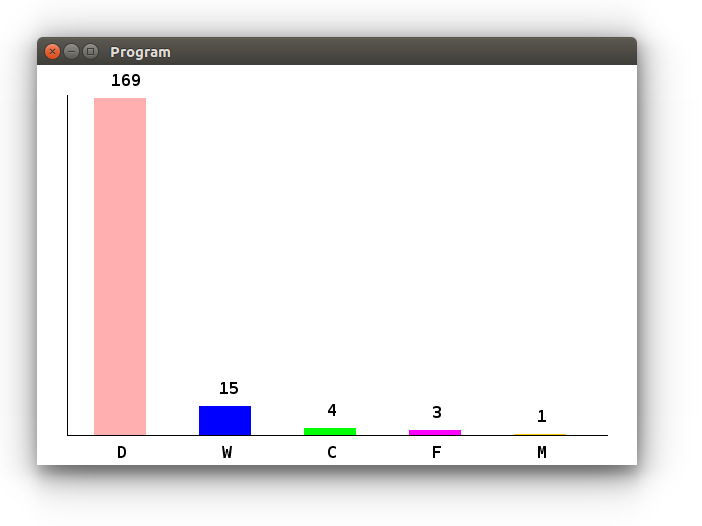
\includegraphics[width=0.95\textwidth]{../img/survey/bar}

\vspace{2em}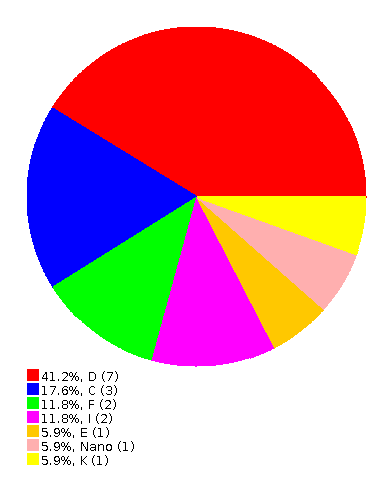
\includegraphics[width=0.7\textwidth]{../img/survey/pie}
\end{minipage}
\end{SlideExtra}

\begin{SlideExtra}{Extraundervisning del 3}
\begin{itemize}
\item  \Alert{Extraundervisning} i \Emph{E:1406} onsdag 21/11 kl 15:15-17:00
\item Hitta dit: \url{http://fileadmin.cs.lth.se/ehus/E1406.pdf}
\item Det finns gott om platser i den salen >70 platser så alla är välkomna
\item Fokus: grundläggande, långsam behandling på begäran, grumliga begrepp etc.
\end{itemize}
\end{SlideExtra}
\fi


%!TEX encoding = UTF-8 Unicode
%!TEX root = ../lect-w06.tex

\Subsection{Scala Build Tool \texttt{sbt} för smidig omkompilering}
\begin{Slide}{Scala Build Tool: \texttt{sbt}}\SlideFontSmall
\begin{itemize}
\item Du kan låta \code{sbt} automatiskt sköta omkompilering och körning vid varje Ctrl+S med kommandot \code{~run}
och enbart omkompilering med \code{~compile}
\begin{REPL}
> sbt              # kör igång sbt i en katalog med .scala-filer
[info] Set current project to hellosbt (in build file:/home/bjornr/tmp/hellosbt/)
[info] sbt server started at 127.0.0.1:5320
sbt:hellosbt> ~run
\end{REPL}
Avsluta med Enter. Om flera \code{main} gör: \code{ ~runMain DettaMainObj}
\item Kod antas finnas direkt i \Emph{aktuell katalog} eller i \code{src/main/scala}
\item Lägg \code{.jar}-filer i en katalog \code{lib} så hamnar de automatiskt på classpath
\item Om du vill: skapa en fil med namnet \code{build.sbt} som konfigurerar \code{sbt}
\begin{Code}
name := "hellosbt"           // bestäm namnet på mitt projekt
scalaVersion := "2.12.6"    // bestäm version av Scala-kompilatorn
\end{Code}
\item Exempel på andra inställningar i \code{bild.sbt}:
\begin{CodeSmall}
scalaSource in Compile := baseDirectory.value / "src"      // bestäm kodkatalog
unmanagedBase := baseDirectory.value / "../annanstans/lib" // bestäm jarfil-katalog
\end{CodeSmall}
Se vidare: Appendix F i kompendiet, \url{http://www.scala-sbt.org/}
\end{itemize}
\end{Slide}


\Lecture{7}{Mängder, tabeller}
%!TEX encoding = UTF-8 Unicode
%!TEX root = ../lect-w07.tex


\Subsection{Kontrollskrivning}

\begin{Slide}{Kontrollskrivning}
Ta med \Alert{legitimation} och \Emph{snabbreferens}, blyertspenna, suddgummi, \Alert{röd} penna till rättningen, förtäring. Ingen mobil. Jackor och väskor vid väggen.
\begin{itemize}
  \item \textbf{Diagnostisk}: vad har du lärt dig hittills?
  \item \textbf{Kamraträttad}: träna på att läsa och bedöma kod
  \item \textbf{Obligatorisk}: sjukdom \Alert{måste} meddelas i förväg
  \item Kan ge \Emph{samarbetsbonus} \Alert{om man har visat samarbetskontrakt}
  %\SlideFontSmall
  \begin{itemize}
    \item[] Max 5p i samarbetsbonus på första ordinarie tentamen, som adderas i slutet av kursen till din tentamenspoäng (max 100) och baseras på \Emph{medelvärdet} av resultaten på kontrollskrivningen i din samarbetsgrupp (se kap ''Anvisningar'' i kompendiet).
  \end{itemize}
\end{itemize}
OBS! Du ska gå på kontrollskrivningen \Alert{även} om du inte har alla labbar godkända.
\end{Slide}

\begin{Slide}{Kontrollskriving -- upplägg}\SlideFontSmall
\begin{itemize}
  \item \textbf{Moment 1}: ca 2 h 15 min: Du löser uppgifterna individuellt
  \item \textbf{Moment 2}: ca 1 h 15 min: Parvis kamratbedömning
  \item \textbf{Moment 3}: ca 30 min: Inspektera din egen skrivning

\item Läs \Alert{noga} igenom instruktionerna på tidigare kontrollskrivning här: 
\url{http://fileadmin.cs.lth.se/pgk/kontroll2018okt30.pdf}
%\url{http://fileadmin.cs.lth.se/pgk/kontroll2017okt24.pdf}

\end{itemize}


\end{Slide}

\begin{Slide}{Plugga själv OCH i din samarbetsgrupp}
\begin{itemize}\SlideFontSmall
  \item Träffas och prata i din samarbetsgrupp om hur ni bäst pluggar \Emph{individuellt} och \Alert{tillsammans} inför kontrollskrivningen för att maximera lärandet i gruppen!

  \item Repetera teorin i läsperiod 1.
  
  \item Repetera lösningar till övningarna och labbarna.

  \item Träna på att koda med papper och penna!

  \item Använd tidigare års kontrollskrivningar: \\ \url{http://cs.lth.se/pgk/examination/}

\pause

\begin{itemize}\SlideFontTiny\vspace{1em}
    \item Observera: 2016 ingick \Emph{arv} i lp1 men sedan 2017 kommer detaljerna om \code{extends} och \code{trait} och \code{abstract} i lp2.
\item Snabbkurs om arv:
\begin{itemize}\SlideFontTiny
\item Med \code{trait Grönsak} skapas en typ med namnet \code{Grönsak} som kan användas som \Emph{bastyp} i en hierarki av typer.
\item Med \code{extends Grönsak} anges att en typ \Alert{är en} \code{Grönsak}:
\end{itemize}

\end{itemize}

\end{itemize}
\begin{Code}
  trait Grönsak { var vikt: Int }   // alla grönsaker har en vikt
  class Gurka(var vikt: Int) extends Grönsak  // Gurka är en Grönsak
  class Tomat(var vikt: Int) extends Grönsak  // Tomat är en Grönsak
\end{Code}
\end{Slide}


% \begin{Slide}{Beställning av tryck av kompendium lp 2}\SlideFontSmall

% \begin{itemize}
% \item Nu är det dags att beställa tryck av kompendiet del 2 som innehåller
% övningar och laborationer inför kommande läsperiod.

% \item Beställ här: \url{http://cs.lth.se/pgk/tryck2}

% \item Priset är till självkostnad och beror på hur många som beställer.
% \item Priset blir max 270kr om färre än 100st beställer
% och ca 165kr om minst 100st beställer.

% \item Svara *snarast* dock senast 19 Oktober kl 0900.

% \item \Alert{Det är himla bra att ha kompendiet på papper, bredvid skärmen speciellt när du jobbar med en IDE med massor av fönster!!}

% \end{itemize}
% \end{Slide}

% \ifkompendium\else
% \begin{SlideExtra}{Grumligt-lådan}
% \begin{itemize}
% \item Jag skickar runt \Emph{Grumligt}-lådan.
% \item Skriv lappar, \Alert{en lapp per begrepp}, som du tycker är \Emph{''grumligt''} och  önskar förstå bättre.
% \item Skicka vidare lådan så fort du är klar.
% \item Sista person i salen lämnar tillbaka lådan till mig på rasten.
% \item Jag kommer att försöka reda ut några högfrekventa grumligheter på kommande föreläsning.
% \end{itemize}
% \end{SlideExtra}
% \fi

\ifkompendium\else
\begin{SlideExtra}{}
  \begin{center}
    \huge\Alert{Lycka till på kontrollskrivningen!}
  \end{center}
\end{SlideExtra}
\fi
%!TEX encoding = UTF-8 Unicode
%!TEX root = ../lect-w07.tex

\Subsection{Samlingar}

\begin{Slide}{Vad är en samling?}
En \Emph{samling} \Eng{collection} är en datastruktur som kan innehålla många element av \Alert{samma typ}.

\pause 
\vspace{2em}\emph{Exempel:} \\Heltalsvektor: \hfill\code{val xs = Vector(2, -1, 3, 42, 0)}

\pause 
{\SlideFontSmall\vspace{2em}Samlingar implementeras med hjälp av klasser. \\ I standardbiblioteken \code{scala.collection} och \code{java.util} finns \Alert{många} \Emph{färdiga samlingar}, så man behöver sällan implementera egna. 

\pause\vspace{0.5em}\emph{Om} man behöver en egen, speciell datastruktur är det ofta lämpligt att skapa en klass som \emph{innehåller} en \emph{färdig} samling och utgå från dess färdiga metoder.

}

\end{Slide}


\begin{Slide}{Typparameter möjliggör generiska samlingar}\SlideFontSmall
Funktioner och klasser kan, förutom vanliga parametrar, även ha \Emph{typparametrar} som skrivs i en egen parameterlista med \Alert{hakparenteser}. En typparameter gör så att funktioner och datastrukturer blir \Emph{generiska} och kan hantera element av \Alert{godtycklig} typ på ett typsäkert sätt. (Mer om detta i w09.)

\begin{REPLnonum}
scala> def strängLängd[T](x: T): Int = x.toString.length
strängLängd: [T](x: T)Int

scala> strängLängd[Double](42.0)  //Double är typargument
res0: Int = 4

scala> strängLängd(42.0) //Kompilatorn härleder T=Double
res1: Int = 4

scala> Vector.empty[Int] //Här kan den ej härleda typen...
res2: scala.collection.immutable.Vector[Int] = Vector()

scala> strängLängd[Vector[Int]](Vector.empty) //...men här
res3: Int = 8
\end{REPLnonum}
\end{Slide}

\begin{Slide}{Hierarki av samlingar i scala.collection}
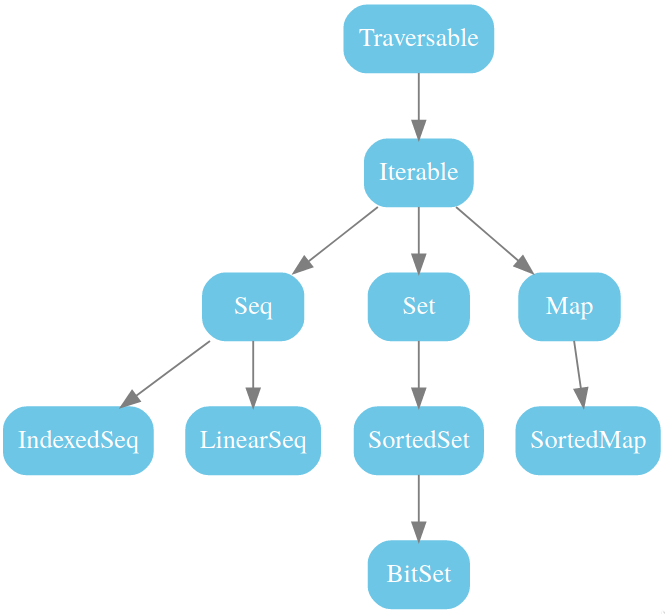
\includegraphics[width=1.0\textwidth]{../img/collection/collection-traits}
\end{Slide}
\noindent Läs mer om Scalas samlingar här: \\ 
\url{http://docs.scala-lang.org/overviews/collections/overview}


\begin{Slide}{Hierarki av samlingstyper i \texttt{scala.collection}}

\begin{multicols}{2}
\begin{tikzpicture}[sibling distance=6.1em,->,>=stealth', inner sep=3pt, %scale=0.5, 
  every node/.style = {shape=rectangle, draw, align=center,font=\small\ttfamily},
  class/.style = {fill=blue!20},
  trait/.style = {rounded corners, fill=red!20}]
  \node[trait] {Traversable}
    child { node[trait] {Iterable} 
      child { node[trait] {Seq} 
       }
      child { node[trait] {Set} 
      }
      child { node[trait] {Map} 
      }
    };
\end{tikzpicture}

\columnbreak
 
{\SlideFontTiny 

\code{Traversable} har metoder som är implementerade med hjälp av: \\
\code{def foreach[U](f: Elem => U): Unit}\\

\vspace{1em}\code{Iterable} har metoder som är implementerade med hjälp av: \\
\code{def iterator: Iterator[A] } 

}

\begin{itemize}\SlideFontTiny 
\item[] \code{Seq}: ordnade i sekvens
\item[] \code{Set}: unika element
\item[] \code{Map}: par av (nyckel, värde)
\end{itemize}


\end{multicols}

{\SlideFontSmall Samlingen \Emph{\texttt{Vector}} är en \code{Seq} som är en \code{Iterable} som är en \code{Traversable}.}
\end{Slide}

\begin{Slide}{Använda \texttt{iterator}}\SlideFontSmall
Med en \code{iterator} kan man \Emph{iterera} med \code{while} över alla element, men endast \Alert{en   gång}; sedan är iteratorn ''förbrukad''. (Men man kan be om en ny.)
\begin{REPL}
scala> val xs = Vector(1,2,3,4)
xs: scala.collection.immutable.Vector[Int] = Vector(1, 2, 3, 4)

scala> val it = xs.iterator
it: scala.collection.immutable.VectorIterator[Int] = non-empty iterator

scala> while (it.hasNext) print(it.next)
1234

scala> it.hasNext
res1: Boolean = false

scala> it.next
java.util.NoSuchElementException: reached iterator end
  at scala.collection.immutable.VectorIterator.next(Vector.scala:674)
\end{REPL}
\Emph{Normalt} behöver man \Alert{inte} använda \code{iterator}: det finns oftast färdiga metoder som gör det man vill, till exempel \code{foreach}, \code{map}, \code{sum}, \code{min} etc.
\end{Slide}

\begin{Slide}{Några användbara metoder på samlingar}\SlideFontTiny
\begin{tabular}{r r l}\hline
\texttt{\Emph{Traversable}} 
  & \code|xs.size| & antal elementet \\
  & \code|xs.head| & första elementet \\
  & \code|xs.last| & sista elementet \\
  & \code|xs.take(n)| & ny samling med de första n elementet \\
  & \code|xs.drop(n)| & ny samling utan de första n elementet \\
  & \code|xs.foreach(f)| & gör \code|f| på alla element, returtyp \code|Unit|\\
  & \code|xs.map(f)| & gör \code|f| på alla element, ger ny samling \\
  & \code|xs.filter(p)| & ny samling med bara de element där p är sant\\
  & \code|xs.groupBy(f)| & ger en \code|Map| som grupperar värdena enligt f\\ 
  & \code|xs.mkString(",")| & en kommaseparerad sträng med alla element\\ \hline
    
\texttt{\Emph{Iterable}} 
  & \code|xs.zip(ys)| & ny samling med par (x, y); ''zippa ihop'' xs och ys \\
  & \code|xs.zipWithIndex| & ger en \code|Map| med par (x, index för x) \\
  & \code|xs.sliding(n)| & ny samling av samlingar genom glidande ''fönster''\\ \hline

\texttt{\Emph{Seq}} 
  & \code|xs.length| & samma som \code|xs.size| \\
  & \code|xs :+ x| & ny samling med x sist efter xs \\
  & \code|x +: xs| & ny samling med x före xs \\ \hline
  
\end{tabular}

\pause
\vspace{0.5em}\Emph{Minnesregel} för \code{+:} och \code{:+  } \Alert{Colon on the collection side}

\pause
Prova fler samlingsmetoder ur snabbreferensen: ~~\url{http://cs.lth.se/quickref}
\end{Slide}



\begin{Slide}{Använda samlingsmetoder}
\begin{REPL}
scala> val tal = Vector(1,4,7,9,42)
tal: scala.collection.immutable.Vector[Int] = Vector(1, 4, 7, 9, 42)

scala> val jämna = tal.filter(_ % 2 == 0)
jämna: scala.collection.immutable.Vector[Int] = Vector(4, 42)

scala> val xs = Vector(("Kim","Smith"), ("Kim", "Jones"), ("Robin", "Smith"))
xs: scala.collection.immutable.Vector[(String, String)] = Vector((Kim,Smith), (Kim,Jones), (Robin,Smith))

scala> val grupperaEfterFörnamn = xs.groupBy(_._1)
grupperaEfterFörnamn: Map[String,Vector[(String, String)]] = 
Map(Kim -> Vector((Kim,Smith), (Kim,Jones)), Robin -> Vector((Robin,Smith)))

scala> val grupperaEfterEfternamn = xs.groupBy(_._2)
grupperaEfterEfternamn: Map[String,Vector[(String, String)]] = 
Map(Jones -> Vector((Kim,Jones)), Smith -> Vector((Kim,Smith), (Robin,Smith)))

\end{REPL}
\end{Slide}




\begin{Slide}{Mer specifik samlingstyper i \texttt{scala.collection}}
Det finns \Alert{mer specifika} \Emph{subtyper} av \code{Seq}, \code{Set} och \code{Map}:
\\ \vspace{1em}

\begin{tikzpicture}[sibling distance=5.8em,->,>=stealth', inner sep=3pt, %scale=0.5, 
  every node/.style = {shape=rectangle, draw, align=center,font=\small\ttfamily},
  class/.style = {fill=blue!20},
  trait/.style = {rounded corners, fill=red!20}]
  \node[trait] {Traversable}
    child { node[trait] {Iterable} 
      child { node[trait, xshift=-2.4cm] {Seq} 
        child { node[trait] {IndexedSeq} }
        child { node[trait] {LinearSeq} }
       }
      child { node[trait, yshift=-0.0cm] {Set} 
        child { node[trait] {SortedSet} }
        child { node[trait] {BitSet} }
      }
      child { node[trait, xshift=1.0cm] {Map} 
        child { node[trait] {SortedMap} }
      }
    };
\end{tikzpicture}

\vspace{0.5em}
\Emph{\texttt{Vector}} är en \Alert{\texttt{IndexedSeq}} medan
\Emph{\texttt{List}} är en \Alert{\texttt{LinearSeq}}.
\end{Slide}

\begin{Slide}{Några oföränderliga och förändringsbara sekvenssamlingar}\SlideFontSmall
\begin{tabular}{r l l}
\texttt{scala.collection.\Emph{immutable}.Seq.} & & \\
 & \code|IndexedSeq.| & \\
 & & \Emph{\texttt{Vector}} \\
 & & \Emph{\texttt{Range}} \\
 & \code|LinearSeq.| & \\
 & & \Emph{\texttt{List}} \\
   & & \Emph{\texttt{Queue}} \\

\texttt{scala.collection.\Alert{mutable}.Seq.} & & \\
 & \code|IndexedSeq.| & \\
 & & \Alert{\texttt{ArrayBuffer}} \\
 & & \Alert{\texttt{StringBuilder}} \\
 & \code|LinearSeq.| & \\
 & & \Alert{\texttt{ListBuffer}} \\
   & & \Alert{\texttt{Queue}} \\
\end{tabular}

Studera samlingars egenskaper här: \href{http://docs.scala-lang.org/overviews/collections/overview}{docs.scala-lang.org/overviews/collections/overview}
\end{Slide}


\begin{Slide}{scala.collection.immutable}
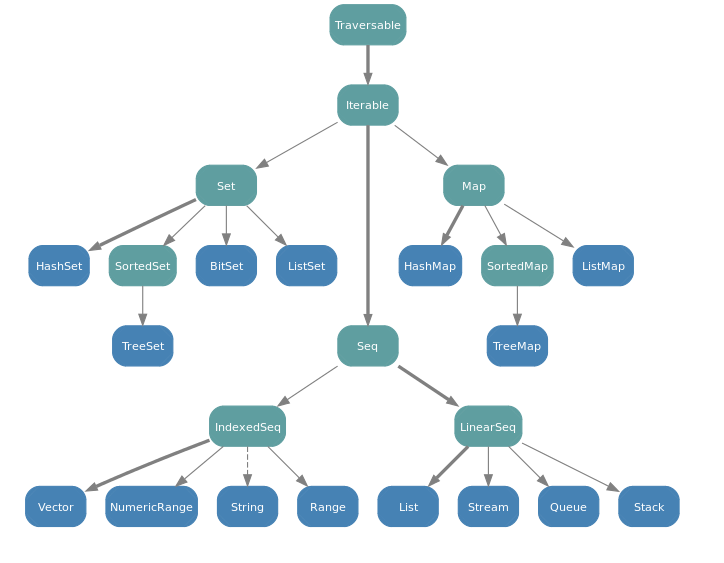
\includegraphics[width=0.82\textwidth]{../img/collection/collection-immutable}
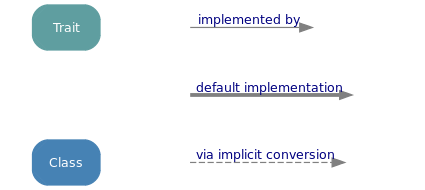
\includegraphics[width=0.33\textwidth]{../img/collection/collection-legend}
\end{Slide}


\begin{Slide}{scala.collection.mutable}
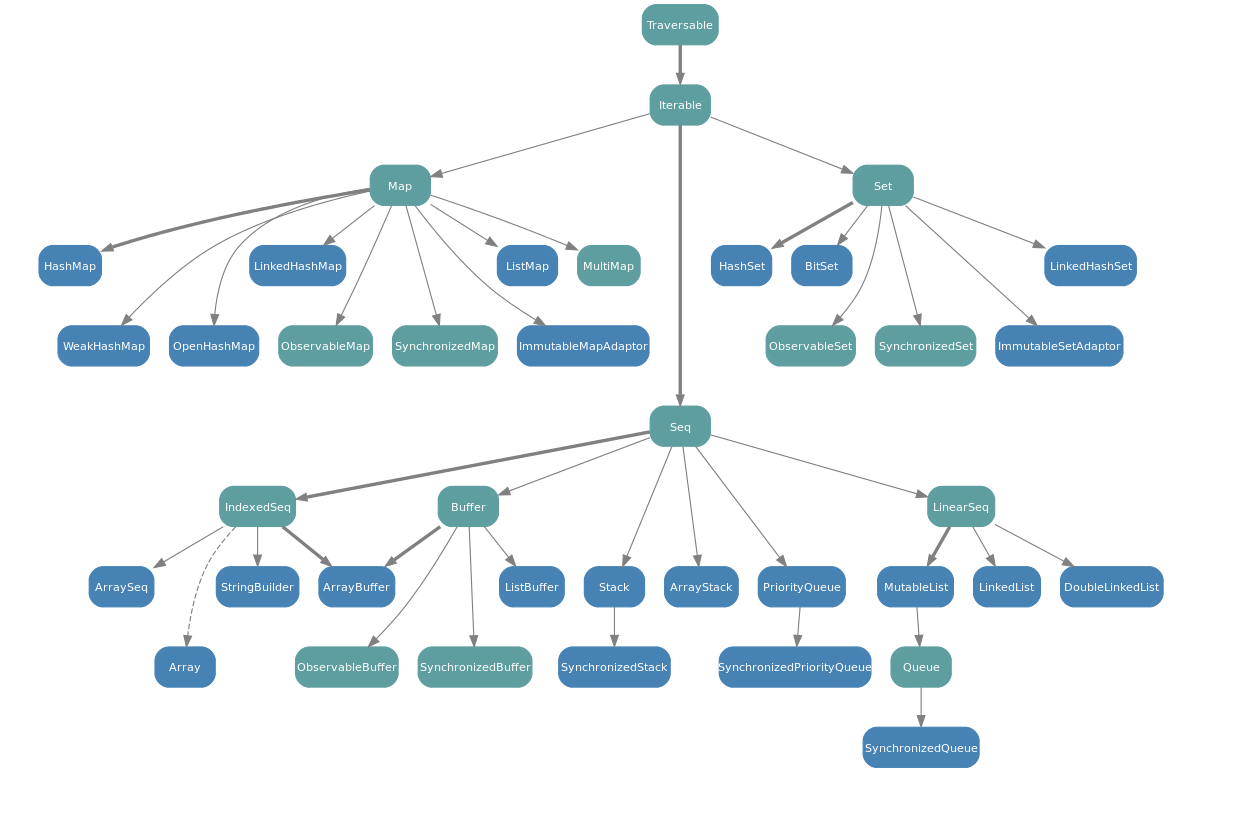
\includegraphics[width=1.05\textwidth]{../img/collection/collection-mutable}
\end{Slide}


\begin{Slide}{Strängar är implicit en \texttt{IndexedSeq[Char]}}\SlideFontSmall
Det finns en så kallad \Emph{implicit konvertering} mellan \code{String} och \code{IndexedSeq[Char]} vilket gör att \Alert{alla samlingsmetoder på \texttt{Seq} även funkar på strängar} och även flera andra smidiga strängmetoder erbjuds \Alert{utöver} de som finns i \href{http://docs.oracle.com/javase/8/docs/api/java/lang/String.html}{\code{java.lang.String}} genom klassen \href{http://www.scala-lang.org/api/current/#scala.collection.immutable.StringOps}{\code{StringOps}}.

\vspace{0.5em}
\begin{REPLnonum}
scala> "hej".  //tryck på TAB och se alla strängmetoder
\end{REPLnonum}
Detta är en stor fördel med Scala jämfört med många andra språk, som har strängar som inte kan allt som andra sekvenssamlingar kan.
\end{Slide}


\begin{Slide}{\texttt{Vector} eller \texttt{List}?}\SlideFontTiny
{\href{http://stackoverflow.com/questions/6928327/when-should-i-choose-vector-in-scala}{stackoverflow.com/questions/6928327/when-should-i-choose-vector-in-scala}}

\begin{enumerate}
\item If we only need to transform sequences by operations like map, filter, fold etc: basically it does not matter, we should program our algorithm generically and might even benefit from accepting parallel sequences. For sequential operations List is probably a bit faster. But you should benchmark it if you have to optimize.

\item If we need a lot of random access and different updates, so we should use vector, list will be prohibitively slow.

\item If we operate on lists in a classical functional way, building them by prepending and iterating by recursive decomposition: use list, vector will be slower by a factor 10-100 or more.

\item If we have an performance critical algorithm that is basically imperative and does a lot of random access on a list, something like in place quick-sort: use an imperative data structure, e.g. ArrayBuffer, locally and copy your data from and to it.
\end{enumerate}
{\href{http://stackoverflow.com/questions/20612729/how-does-scalas-vector-work}{stackoverflow.com/questions/20612729/how-does-scalas-vector-work}}\\
Mer om tids- och minneskomplexitet i fördjupningskursen och senare kurser.
\end{Slide}



\begin{Slide}{Mängd: snabb innehållstest, garanterat dubblettfri}\SlideFontSmall
En \Emph{mängd} \Eng{set} är en samling som \Alert{inte} kan innehålla \Alert{dubbletter} och som är snabb på att avgöra om ett element \Alert{finns eller inte} i mängden.

\begin{REPL}
scala> var veg = Set.empty[String]
veg: scala.collection.immutable.Set[String] = Set()

scala> veg = veg + "Gurka"
veg: scala.collection.immutable.Set[String] = Set(Gurka)

scala> veg = veg ++ Set("Broccoli", "Tomat", "Gurka")
veg: scala.collection.immutable.Set[String] = Set(Gurka, Broccoli, Tomat)

scala> veg.contains("Gurka")
res0: Boolean = true

scala> veg.apply("Gurka")   // samma som contains
res1: Boolean = true

scala> veg("Morot")
res2: Boolean = false
\end{REPL}

\end{Slide}

\begin{Slide}{Den fantastiska nyckel-värde-tabellen \texttt{Map}}\SlideFontSmall
\begin{itemize}
\item En \Emph{nyckel-värde-tabell} \Eng{key-value table} är en slags generaliserad vektor där man kan ''indexera'' med godtycklig typ. 

\item Kallas öven \href{https://sv.wikipedia.org/wiki/Hashtabell}{\Emph{hashtabell}} \Eng{hash table}, \Emph{lexikon} \Eng{dictionary} eller kort och gott \Emph{mapp} \Eng{map},

\item En hashtabell är en \Emph{samling av par}, där varje par består av en \Alert{unik} \Emph{nyckel} och ett tillhörande \Emph{värde}. 

\item Om man vet nyckeln kan man få fram värdet \Alert{snabbt}, på liknande sätt som indexering sker i en vektor om man vet heltalsindex. 

\item Denna datastruktur är \Alert{mycket användbar} och liknar en enkel databas.
\end{itemize}
\begin{REPL}
scala> val födelse = Map("C" -> 1972,  "C++" -> 1983, "C#" -> 2000, 
  "Scala" -> 2004, "Java" -> 1995, "Javascript" -> 1995, "Python" -> 1991)

födelse: scala.collection.immutable.Map[String,Int] = Map(Scala -> 2004, C# -> 2000, Python -> 1991, Javascript -> 1995, C -> 1972, C++ -> 1983, Java -> 1995)
  
scala> födelse.apply("Scala")
res0: Int = 2004

scala> födelse("Java")
res1: Int = 1995

\end{REPL}
\end{Slide}

\begin{Slide}{Exempel nyckel-värde-tabell}
\begin{REPL}
scala> val färg = Map("gurka" -> "grön", "tomat"->"röd", "aubergine"->"lila")
färg: scala.collection.immutable.Map[String,String] = 
  Map(gurka -> grön, tomat -> röd, aubergine -> lila)

scala> färg("gurka")
res0: String = grön

scala> färg.keySet
res1: scala.collection.immutable.Set[String] = Set(gurka, tomat, aubergine)

scala> val ärGrönSak = färg.map(elem => (elem._1, elem._2 == "grön"))
ärGrönSak: Map[String,Boolean] = Map(gurka -> true, tomat -> false, aubergine -> false)

scala> val baklängesFärg = färg.mapValues(s => s.reverse)
baklängesFärg: Map[String,String] = Map(gurka -> nörg, tomat -> dör, aubergine -> alil)

\end{REPL}
\begin{itemize}
\item \code{xs.keySet} ger en mängd av alla nycklar
\item \code{xs.map(f)} mappar funktionen f på alla par av (key, value)
\item \code{xs.mapValues(f)} mappar funktionen f på alla värden 
\end{itemize}

\end{Slide}

\begin{Slide}{Metoderna zipWithIndex, groupBy och mapValues}
\begin{REPL}
scala> val högaKort = Vector("Knekt", "Dam", "Kung", "Äss")

scala> val kortIndex = högaKort.zipWithIndex.toMap
kortIndex: Map[String,Int] = Map(Knekt -> 0, Dam -> 1, Kung -> 2, Äss -> 3)

scala> kortIndex("Kung") > kortIndex("Knekt") 
res0: Boolean = true

scala> val xs = Vector(("Kim","Smith"), ("Kim", "Jones"), ("Robin", "Smith"))
xs: Vector[(String, String)] = Vector((Kim,Smith), (Kim,Jones), (Robin,Smith))

scala> val grupperaEfterFörnamn = xs.groupBy(_._1)
grupperaEfterFörnamn: Map[String,Vector[(String, String)]] = 
Map(Kim -> Vector((Kim,Smith), (Kim,Jones)), Robin -> Vector((Robin,Smith)))

scala> val grupperaEfterEfternamn = xs.groupBy(_._2)
grupperaEfterEfternamn: Map[String,Vector[(String, String)]] = 
Map(Jones -> Vector((Kim,Jones)), Smith -> Vector((Kim,Smith), (Robin,Smith)))

scala> val frekvens = xs.groupBy(_._1).mapValues(_.size)
frekvens: Map[String,Int] = Map(Kim -> 2, Robin -> 1)
\end{REPL}
\end{Slide}


\begin{Slide}{Speciella metoder på förändringsbara samlingar}\SlideFontSmall
Både \code{Set} och \code{Map} finns i \Alert{förändringsbara} varianter med extra metoder för uppdatering av innehållet ''på plats'' utan att nya samlingar skapas.
\begin{REPL}
scala> import scala.collection.mutable

scala> val ms = mutable.Set.empty[Int]
ms: scala.collection.mutable.Set[Int] = Set()

scala> ms += 42
res0: ms.type = Set(42)

scala> ms += (1, 2, 3, 1, 2, 3); ms -= 1
res1: ms.type = Set(2, 42, 3)

scala> ms.mkString("Mängd: ", ", ", s" Antal: ${ms.size}")
res2: String = Mängd: 1, 2, 42, 3 Antal: 4

scala> val ordpar = mutable.Map.empty[String, String]
scala> ordpar += ("hej" -> "svejs", "abra" -> "kadabra", "ada" -> "lovelace")
scala> println(ordpar("abra"))
kadabra
\end{REPL}
\end{Slide}

\begin{Slide}{Fler exempel på samlingsmetoder}
Exempel: räkna bokstäver i ord.  \\
Undersök vad som händer i REPL:
\begin{Code}[basicstyle=\SlideFontSize{9}{13}\ttfamily]
val ord = "sex laxar i en laxask sju sjösjuka sjömän" 
val uppdelad = ord.split(' ').toVector
val ordlängd = uppdelad.map(_.length)
val ordlängdMap = uppdelad.map(s => (s, s.size)).toMap
val grupperaEfterFörstaBokstav = uppdelad.groupBy(s => s(0))
val bokstäver = ord.toVector.filter(_ != ' ')
val antalX = bokstäver.count(_ == 'x')
val grupperade = bokstäver.groupBy(ch => ch)
val antal = grupperade.map(kv => (kv._1, kv._2.size))
val sorterat = antal.toVector.sortBy(_._2)
val vanligast = antal.maxBy(_._2)
\end{Code}
\end{Slide}


\begin{Slide}{Jobba med föränderlig samling lokalt; \\ returnera oföränderlig samling när du är klar}
\SlideFontSmall
Om du vill implementera en imperativ algoritm med en föränderlig samling:\\ 
Gör gärna detta \Alert{lokalt} i en \Alert{förändringsbar} samling och returnera sedan en \Emph{oföränderlig} samling, genom att köra t.ex. \code{toSet} på en mängd, eller \code{toMap} på en hashtabell, eller \code{toVector} på en \code{ArrayBuffer} eller \code{Array}.

\begin{REPL}
scala> :paste
def kastaTärningTillsAllaUtfallUtomEtt(sidor: Int = 6) = {
  val s = scala.collection.mutable.Set.empty[Int]
  var n = 0
  while (s.size < sidor - 1) {
    s += (math.random * sidor + 1).toInt
    n += 1
  }
  (n, s.toSet)
}
scala> kastaTärningTillsAllaUtfallUtomEtt()
res0: (Int, scala.collection.immutable.Set[Int]) = (13,Set(5, 1, 6, 2, 3))

\end{REPL}

\end{Slide}







\Lecture{8}{Matriser, typparametrar}
%!TEX encoding = UTF-8 Unicode
%!TEX root = ../lect-week08.tex

%%%

\ifkompendium\else

\Subsection{Justeringar av kursupplägg}

\begin{Slide}{Justeringar av kursupplägg baserat på feedback}\SlideFontSmall
  Under instuderingsveckan har vi gjort följande \Emph{kursutveckling} baserat på feedback. (Alltså gäller \Alert{inte} upplägget som beskrivs i kompendium del 1 för andra läsperioden.)
  \begin{itemize}
    \item Två labbar är omgjorda från grunden och är nu mindre omfattande och en labb är väsentligt förenklad för att minska arbetsbelastningen.
    \item Omgjorda labbar:
    \begin{itemize}\SlideFontSmall
      \item \code{w08_maze} är väsentligt \Emph{förenklad} och förtydligad.
      \item \code{w10_music} helt ny och \Emph{förenklad} (ersätter \code{chords_team}).
      \item \code{w11_javatext} helt ny och \Emph{friare} (ersätter \code{lthopoly_team} men om (några) i samarbetsgruppen vill kan de välja att göra \code{lthopoly_team} i stället för \code{javatext}).
    \end{itemize}
    \item \code{w12_survey} som kombinerar matriser med sortering är ändrad till att vara \Emph{valfri} och \Alert{rekommenderad} för alla de som satsar på \Alert{betyg 4 el. 5}.

    \item I villkoret för att få tenta ingår alltså labb \code{1-11}, men inte 12.
  \end{itemize}
\end{Slide}

\Subsection{Kontrollskrivning}

\begin{Slide}{Resultat på kontrollskrivning 2016}
\pgfplotstableread[row sep=\\,col sep=&]{
    poäng & kamraträttat & korrigerat\\
    0     & 18  & 15\\
    1     & 29  & 29 \\
    2     & 17  & 15\\
    3     & 20  & 21 \\
    4     & 21  & 18 \\
    5     & 8   & 15 \\
    }\dataSexton

\begin{minipage}{0.6\textwidth}
\hspace*{-0.65cm}\begin{tikzpicture}[scale=0.9, every node/.style={scale=0.9}]
    \begin{axis}[
            ybar,
            symbolic x coords={0,1,2,3,4,5},
            xtick=data,
            nodes near coords,
            nodes near coords align={vertical},
            legend style={at={(0.5,1)},anchor=south,legend columns=-1,draw=none},
            ymin=0,ymax=35,
            ylabel={Antal},
            xlabel={Poäng},
        ]
        \addplot table[x=poäng,y=kamraträttat]{\dataSexton};
        \addplot table[x=poäng,y=korrigerat]{\dataSexton};
        \legend{kamraträttat, korrigerat}
    \end{axis}
\end{tikzpicture}
\end{minipage}%
\begin{minipage}{0.35\textwidth}
\begin{itemize}\SlideFontTiny
\item[] Totalt: 107 st (100\%)
\item[] 4 -- 5: 33st (29\%)
\item[] 3 -- 5: 54st (48\%)
\item[] 0 -- 2: 59st (52\%)
\item[] 0 -- 1: 44st (39\%)
\end{itemize}
\end{minipage}%
\end{Slide}



\begin{Slide}{Resultat på kontrollskrivning 2017}
\pgfplotstableread[row sep=\\,col sep=&]{
    poäng & kamraträttat & korrigerat\\
    0     & 10  & 4\\
    1     & 28  & 31 \\
    2     & 20  & 19\\
    3     & 22  & 21 \\
    4     & 17  & 18 \\
    5     & 17  & 22 \\
    }\dataSjutton

\begin{minipage}{0.6\textwidth}
\hspace*{-0.65cm}\begin{tikzpicture}[scale=0.9, every node/.style={scale=0.9}]
    \begin{axis}[
            ybar,
            symbolic x coords={0,1,2,3,4,5},
            xtick=data,
            nodes near coords,
            nodes near coords align={vertical},
            legend style={at={(0.5,1)},anchor=south,legend columns=-1,draw=none},
            ymin=0,ymax=35,
            ylabel={Antal},
            xlabel={Poäng},
        ]
        \addplot table[x=poäng,y=kamraträttat]{\dataSjutton};
        \addplot table[x=poäng,y=korrigerat]{\dataSjutton};
        \legend{kamraträttat, korrigerat}
    \end{axis}
\end{tikzpicture}
\end{minipage}%
\begin{minipage}{0.35\textwidth}
\begin{itemize}\SlideFontTiny
\item[] Totalt: 115 st (100\%) korrigerat:
\item[] 4 -- 5: 40st (34\%)
\item[] 3 -- 5: 61st (53\%)
\item[] 0 -- 2: 54st (47\%)
\item[] 0 -- 1: 35st (30\%)
\end{itemize}
\end{minipage}%
\end{Slide}




% \begin{Slide}{Genomgång av kontrollskrivning}
% \begin{itemize}
% \item Förstå uppgiften
%
% \item Strategi för lösning
%
% \item Skapa lösning iterativt
%
% \item Kontrollera lösning
% \end{itemize}
% \end{Slide}



\Subsection{REBOOT CAMP}

\begin{Slide}{Reboot Camp och Extraundervisning}

\begin{itemize}
  \item
  Träffas i din samarbetsgrupp och organisera själva en \Emph{REBOOT CAMP} baserat på kontrollskrivningsresultatet.

\begin{itemize}
  \item
  3-5: GRATTIS! Bli ännu starkare!
  \item
  0-2: Fixa trösklar och luckor!
\end{itemize}

\item \Alert{EXTRAUNDERVISNING} för de som har det \Alert{allra svårast}
\begin{itemize}
  \item Anmälan sker genom att komma till\\\Emph{E:2116} kl 13-15 på tordag den 2 november.
%  \item De som fick 0--1 på kontrollskrivningen har förtur
%  \item De med 0 på kontrollen rekommenderas starkt att delta!
\end{itemize}

\end{itemize}


\vspace{0.5em} \Emph{STAY CALM} \\\vspace{0.5em} \Alert{GET ON TRACK}
\end{Slide}

%
% \begin{Slide}{Omplanering: w08 = REBOOT CAMP}\SlideFontSmall
% Det är \Alert{för många} som ligger \Alert{för långt efter}: \\
% \Emph{Vi måste göra något!}
% \begin{itemize}
% \item Omplanering: w08 = REBOOT CAMP
% \begin{itemize}\SlideFontTiny
% \item \Alert{GE JÄRNET} för att stärka dig inför resten av kursen!
% \item Noggrann genomgång av kontrollskrivning
% \item Gör självdiagnostik och kämpa dig över trösklar och fyll igen luckor
% \item Slipa dina inlärningsverktyg!
% \item Resurstider: \code{reboot-init}: \Emph{planera, arbeta}
% \item Labb: \code{reboot-check}: \Emph{visa hur det går, arbeta}
% \end{itemize}
% \item Vi senarelägger alla kvarvarande labbar en vecka så att w08 frigörs;
%  lab \code{chords-team} görs alltså i vecka w09 etc.
%
% \item Sista labben \code{life} omdefinieras till att ingå bland projektalternativen i slutet av kursen (man får ändå öva på matriser på lab \code{maze})
%
% \item Stoffet i veckorna w12 \& w13 slås ihop och minskas ned
%
% \item Övn threads blir frivilligt extramaterial och ingår ej i examinationen.
%
% \end{itemize}
% \end{Slide}


%\Subsection{Slipa verktygen}



% \begin{Slide}{Slipa verktygen}
% För dig som har det \Alert{svårt}:
% \begin{itemize}
% \item Man kan inte lära sig ett språk bara genom att \Alert{passivt} läsa
% \item Om du inte börjat än: nu måste du verkligen börja skriva, prata, uppfinna, konstruera, göra själv, vara \Emph{aktiv}, ...
% \end{itemize}
% För dig som har det \Emph{lätt}:
% \begin{itemize}
% \item Om du utmanar dig når du \Emph{mycket} längre
% \item Analysera dina styrkor och svagheter
% \item Utveckla din studieteknik och problemlösningsförmåga
% \end{itemize}
% \end{Slide}
%
% \begin{Slide}{Vad avgör studieframgång?}
% Studieteknik, Attityd till sina studier, (Talang)
% \url{https://www.youtube.com/watch?v=gSbpRjxYq24}
%
% \vspace{2em} Att repetera:
% \url{https://www.youtube.com/watch?v=mmAmsaRH_VA}
%
% \vspace{2em} Att planera:
% \url{https://www.youtube.com/watch?v=g2BTFzYnNNY}
% \end{Slide}

\begin{Slide}{Självdiagnostik och planering}
\begin{itemize}
%\item Hur lär jag mig bäst?
\item Vad behöver jag extra träning på?
\begin{itemize}
\item Vad hade jag lätt resp. svårt för på kontrollskrivingen?
\item Vilka är mina \Alert{trösklar}? Extra svårt?
\item Vilka är mina \Alert{luckor}? Inte provat alls?
\item Vilka är mina \Emph{intressen}? Hur fördjupa mig?
\end{itemize}
% \item Hur ska jag planera min REBOOT CAMP?
% \begin{itemize}
% \item Gör ett schema dag för dag.
% \item Vilken undervisning ska jag gå på?
% \item Du som fick 0-2: gå på minst 2 resurstider.
% \item Hur mycket fritid kan jag frigöra till REBOOT CAMP?
% \end{itemize}
\end{itemize}
\end{Slide}



% \begin{Slide}{Strategier för problemlösning i programmering}
% \begin{itemize}
% \item Börja med ett litet men fungerande program; ta sedan många små steg och testa hela tiden att det fungerar
% \item Om problemet är för \Alert{svårt}:\\ lös först ett \Emph{lättare}, relaterat problem
% \item Dela upp problemet i delar
% \begin{itemize}
% \item \code{val braNamn = delresultat}
% \item \code{def delLösning = algoritm som löser delproblem}
% \item \code{??? // inte klart än}
% \end{itemize}
% \item Problemlösning är inte linjärt: du måste kunna knåpa på ditt program i olika ''ändar''; skriva lite här och där; stoppa in; flytta runt; ändra
% \end{itemize}
% \end{Slide}
%
% \begin{Slide}{Strategier för att komma över trösklar}\SlideFontSmall
% \Alert{tröskel} == jag har svårt att begripa och komma vidare; kan ej själv konstruera
%
% \begin{itemize}\SlideFontTiny
% \item Du måste först \Emph{identifiera tröskeln} och tydligt formulera vad du inte förstår eller inte kan klara av att själv skapa.
%
% \item Du måste hitta ett sätt att \Emph{konkretisera} begrepp och \Emph{visualisera} vad som händer \\
% Använd analogier: kaffekvarnen för funktion, stämpla för instansiering, etc.
%
% \item Använd flera exempel på samma sak: försök se \Emph{mönster} \\
% Exempel: Tomat och Gurka är Grönsak; Student och Lärare är Person. \\ Lär dig pseudokodexempel på vanliga algoritmer i kompendiet utantill!
%
% \item Gör \Emph{enklast möjliga} exempel som du exekverar: \\ Skapa en enkel klass med bara en heltalsmedlem och ''lek'' med den.
%
% \item Bygg vidare på det du lär dig och \Emph{utvidga} stegvis med större exempel.\\ Exekvera allt större kod som du själv skriver!
%
% \item \Emph{Avancera}: Kombinera med begrepp du redan känner. Exekvera!
%
% \end{itemize}
% Utgå från det du vet om hur just \Emph{du} lär dig bäst. Hur ska du vara \Alert{aktiv}? \\ Rita. Prata. Skriv sammanfattningar. Skapa egna program. ...
% \end{Slide}
%
% \begin{Slide}{Uppdrag under rasten}
% \begin{itemize}
% \item Tala med med en eller två som är \Emph{ungefär på din nivå} med ledning av resultatet på kontrollskrivningen. (Eller skriv ner för dig själv om du helst vill vara ensam)
%
% \item 5 minuter var: berätta för den andre om...
% \begin{itemize}
%  \item dina trösklar: vad är extra svårt?
%  \item dina luckor: vad har jag inte ens provat själv?
%  \item dina fördjupningsintressen: vad vill jag veta mer om?
%  \item övningar och laborationer som behöver kompletteras
% \end{itemize}
% \item \Alert{Fastna inte} i orsaker/ursäkter till situationen: \Emph{utgå från nuläget} och  indentifiera trösklar/luckor/fördjupning
% \end{itemize}
% \end{Slide}
%
%
% \begin{Slide}{Tillbaka efter rasten:}
% %Påbörja detta arbete som du sedan fortsätter med i eftermiddag/kväll:
% \begin{itemize}
% \item Gör en lista på vad just \Alert{du} behöver göra för att \Emph{slipa dina verktyg} i programmering?
% \item För varje begreppslista i w01-w07:
% \begin{itemize}
% \item Välj ut några begrepp som är viktiga för dig att träna mer på.
% \item Välj ut några övningar som är kopplade till begreppen.
% \item Gör en \Emph{prio-lista} för begreppen/övningarna.
% \item Planera ditt arbete för veckan:
% \begin{itemize}
% \item Övningar
% \item Ev. labbar att komplettera
% \end{itemize}
% \end{itemize}
% \item Ta med dig \Emph{prio-listan} till \Alert{resurstiderna} och diskutera med handledare!
% \end{itemize}
% \end{Slide}
%
%
% %\Subsection{Prioritera dina uppgifter}
%
% \begin{Slide}{Inventering av trösklar, luckor, fördjupning}
% I ditt arbete med att identifiera trösklar, luckor, fördjupning kan du använda:
% \begin{itemize}
% \item Kontrollskrivningen
% \item Målen på övningarna
% \item Begreppslistan i varje modul
% \end{itemize}
% Gör en inventering och markera det du har någorlunda koll på och det du tycker är extra svårt (tröskel) eller sådant du missat (luckor). Om du är redo för fördjupning markera intressanta delar att lära dig mer om.
% \end{Slide}
%
% \begin{Slide}{Prioritera och definiera dina anpassade träning}
% \begin{itemize}
% \item Gör klart eventuella labbar som behöver kompletteras.
% \item Välj en lagom stor mängd övningar ur kompendiet som hjälper dig med trösklar och luckor. Modifiera gärna övningarna efter dina behov.
% \item Definiera ett program du ska jobba med fram till och med reboot-check.
% \end{itemize}
% \end{Slide}

% \begin{Slide}{Hur blir jag godkänd på reboot-check?}
% \begin{itemize}
% \item Förbered en kort genomgång som du ska göra när du får tid med handledare:
% \begin{itemize}
% \item Vilka trösklar/luckor/fördjupningar har du identifierat?
% \item Vad har du gjort under veckan?
% \item Visa ditt program som du jobbar med under labben och förklara hur programmet hänger ihop med dina trösklar/luckor/fördjupningar?
% \end{itemize}
% \item Använd tiden under labben till något vettigt;  jobba vidare på ditt eget program medan du väntar.
% \end{itemize}
% Du blir godkänd om du kan resonera om kopplingen mellan dina behov och dina åtgärder.
% \end{Slide}

\fi

%!TEX encoding = UTF-8 Unicode
%!TEX root = ../lect-w08.tex

% \Subsection{TODO TABORT Integrerad utvecklingsmiljö (IDE)}

% \begin{Slide}{\TODO TABORT Välja IDE}\SlideFontSmall
% \begin{itemize}
% \item En \Emph{integrerad utvecklingsmiljö} \Eng{Integrated Development Environment, IDE} innehåller \\ editor + kompilator + debugger + en massa annat\\och gör utvecklingen enklare när man lärt sig alla finesser.

% \item Läs om vad en IDE kan göra i appendix.

% \pause

% \item På LTH:s datorer finns tre populära IDE installerade:
% \begin{enumerate}\SlideFontSmall

% \item \Emph{VS Code} med tillägget Metals. \Alert{Rekommenderas!}
% \begin{REPL}[numbers=none]
% > code
% \end{REPL}


% \item \Emph{IntelliJ IDEA} med Scala-plugin. Välj denna om du vill ha en IDE som är mer avancerad och är sugen på att lära dig något nytt.
% \begin{REPL}[numbers=none]
% > idea
% \end{REPL}

% \item \Emph{Eclipse} med plugin \Emph{ScalaIDE} förinstallerad, men rekommenderas ej då den ligger efter i Scala-version.
% \begin{REPL}[numbers=none]
% > scalaide
% \end{REPL}

% \end{enumerate}
% %Läs mer om dessa i appendix.
% %  innan du väljer vilken du vill lära dig.
% % \\Där står även hur du installerar dem på din egen dator.
% % \\IntelliJ anses av många för tillfället ha det bästa Scala-stödet, men är du van vid Eclipse så kanske du vill använda ScalaIDE.
% \end{itemize}
% \end{Slide}

% \begin{Slide}{\TODO SKA HANDLA OM DEBUG i VS Code med Scala-plugin Metals}
% 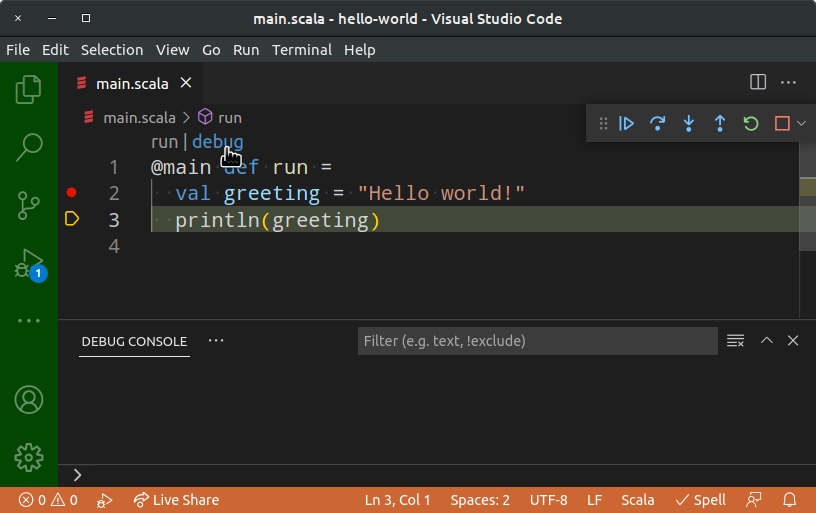
\includegraphics[width=\textwidth]{../img/vscode-debug.png}
% \end{Slide}
  

% \begin{Slide}{IntelliJ IDEA med Scala-plugin}
% 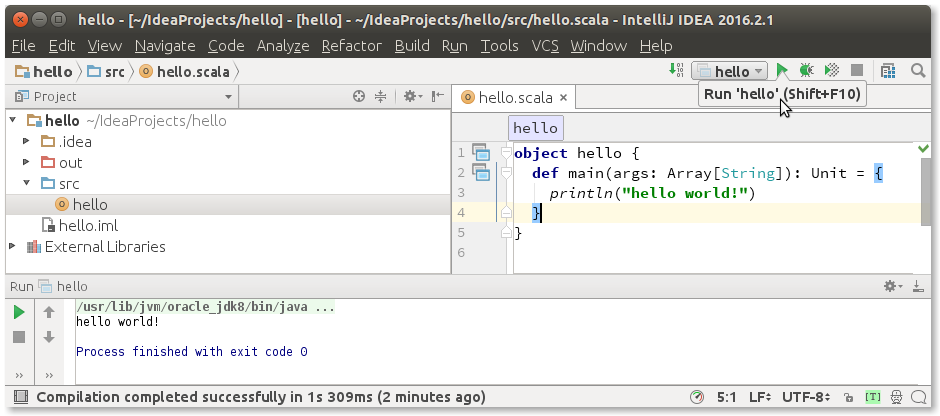
\includegraphics[width=\textwidth]{../img/intellij/idea-hello.png}
% \end{Slide}

% \begin{Slide}{Eclipse med ScalaIDE}
% 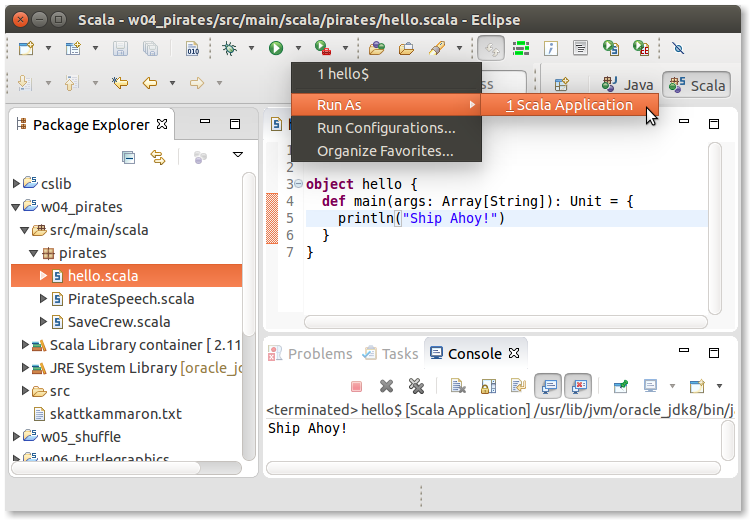
\includegraphics[width=\textwidth]{../img/eclipse/eclipse-pirates-hello.png}
% \end{Slide}


%!TEX encoding = UTF-8 Unicode
%!TEX root = ../lect-w08.tex

%%%

\Subsection{Veckans labb: \texttt{life}}

\begin{Slide}{Veckans labb: \texttt{life}}
\begin{minipage}{0.52\textwidth}
  \setlength{\leftmargini}{0pt}

\begin{itemize}
  \SlideFontSmall
\item Universum är en binär matris av \Emph{celler} där \Emph{levande} celler representeras med \code{true} och \Alert{döda} med \code{false}.
\item Följande regler gäller för \Emph{nästa generation} celler i universum:
\begin{itemize}\SlideFontTiny
  \item \textbf{Fortlevnad}: en levande cell med 2 eller 3 grannar \Emph{lever vidare}
  \item \textbf{Död}: en levande cell med färre än 2 eller fler än 3 grannar \Alert{dör}
  \item \textbf{Födelse}: en död cell med exakt tre grannar föds
\end{itemize}
\item Övning \code{matrices} uppgift 5: skapa en generisk \code{case class Matrix[T]}
\item På labben: använd \code{Matrix[Boolean]}
\end{itemize}

\end{minipage}%
\begin{minipage}{0.5\textwidth}
  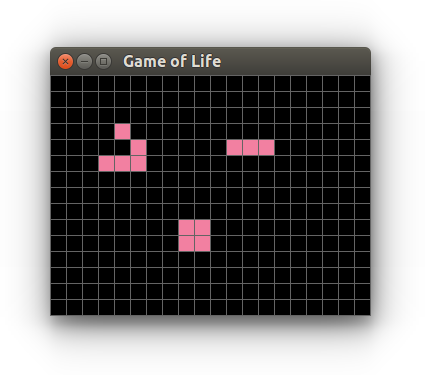
\includegraphics[width=1.0\textwidth]{../img/glider-blinker-block}

  \begin{itemize}\SlideFontTiny
  \item Du ska simulera \emph{Game of Life} i ett \code{introprog.PixelWindow}
  \item Fördjupning:\\{\SlideFontTiny\url{https://en.wikipedia.org/wiki/Conway%27s_Game_of_Life}}
  \end{itemize}
\end{minipage}%

\end{Slide}






\Subsection{Matriser}

\begin{Slide}{Vad är en matris?}\SlideFontSmall
\begin{itemize}

\item En \Emph{matris} inom \Alert{matematiken} innehåller \Emph{rader} och \Emph{kolumner}\footnote{även kallade \emph{kolonner}} med tal.

\item I en \Alert{matematisk} matris har alla rader \Emph{lika många} element och

\item även alla kolumner har \Emph{lika många} element.

\item En matris av dimension $2\times{}5$ har $2 \cdot 5 = 10$ stycken element.

\item Exempel på en matematisk matris av dimension $2\times{}5$:
\[
M_{2,5}=
  \begin{pmatrix}
    5 & 2 & 42 & 4 & 5 \\
    3 & 4 & 18 & 6 & 7
  \end{pmatrix}
\]
\end{itemize}
\end{Slide}

\begin{Slide}{Indexering i en matris}\SlideFontSmall
\begin{itemize}

  \item En matris av dimension $m\times{}n$ har $m \cdot n$ stycken element.

  \item En matris $A_{m,n}$ av dimension $m\times{}n$ ritas inom matematiken ofta så här:

  \[
  A_{m,n} =
   \begin{pmatrix}
    a_{1,1} & a_{1,2} & \cdots & a_{1,n} \\
    a_{2,1} & a_{2,2} & \cdots & a_{2,n} \\
    \vdots  & \vdots  & \ddots & \vdots  \\
    a_{m,1} & a_{m,2} & \cdots & a_{m,n}
   \end{pmatrix}
  \]


\item Matrisindexering inom matematiken sker ofta från $1$, men ofta från $0$ i datorprogram.

\item Vad har talet $42$ för index i matrisen $M_{2,5}$ nedan?
\begin{itemize}\SlideFontTiny
  \item[--] Inom matematiken?
  \item[--] I Scala och Java och många andra språk?

  \[
  M_{2,5}=
    \begin{pmatrix}
      5 & 2 & 42 & 4 & 5 \\
      3 & 4 & 18 & 6 & 7
    \end{pmatrix}
  \]
\end{itemize}
\end{itemize}
\end{Slide}

\begin{Slide}{En matris med array av arrayer}
Inom programmering används ordet \Emph{matris} ofta för att beteckna en \Alert{nästlad struktur} i två dimensioner, till exempel en instans av typen \code{Array[Array[Int]]}
\begin{REPL}
scala> val xss = Array(Array(5,2,42,4,5),Array(3,4,18,6,7))
xss: Array[Array[Int]] = Array(Array(5, 2, 42, 4, 5), Array(3, 4, 18, 6, 7))
\end{REPL}
\pause
Man indexerar i en nästlad sekvens med upprepad \code{apply}:
\begin{REPL}
scala> xss(0)(2)
res0: ???                   // Vad är typ och värde?

scala> xss.apply(0).apply(2)
res1: ???                   // Vad är typ och värde?

scala> xss(0)
res2: ???                   // Vad är typ och värde?
\end{REPL}

\end{Slide}

\begin{Slide}{En matris med array av arrayer}
Inom programmering används ordet \Emph{matris} ofta för att beteckna en \Alert{nästlad struktur} i två dimensioner, till exempel en instans av typen \code{Array[Array[Int]]}
\begin{REPL}
scala> val xss = Array(Array(5,2,42,4,5),Array(3,4,18,6,7))
xss: Array[Array[Int]] = Array(Array(5, 2, 42, 4, 5), Array(3, 4, 18, 6, 7))
\end{REPL}

Man indexerar i en nästlad sekvens med upprepad \code{apply}:
\begin{REPL}
scala> xss(0)(2)
res0: Int = 42

scala> xss.apply(0).apply(2)
res1: Int = 42

scala> xss(0)
res2: Array[Int] = Array(5, 2, 42, 4, 5)
\end{REPL}
\end{Slide}

\begin{Slide}{Uppdatering av en förändringsbar nästlad struktur}
Man kan förändra en array av arrayer ''på plats'' med tilldelning:
\begin{REPL}
scala> val xss = Array(Array(5,2,42,4,5),Array(3,4,18,6,7))

scala> xss(0)(0) = 100

scala> xss
res0: ???

scala> xss(0)(2) = xss(0)(2) - 1

scala> xss
res1: ???

scala> xss(1) = Array.fill(5)(-1)

scala> xss
res2: ???
\end{REPL}
\end{Slide}

\begin{Slide}{Uppdatering av en förändringsbar nästlad struktur}
Man kan förändra en array av arrayer ''på plats'' med tilldelning:
\begin{REPL}
scala> val xss = Array(Array(5,2,42,4,5),Array(3,4,18,6,7))

scala> xss(0)(0) = 100

scala> xss
res0: Array[Array[Int]]=Array(Array(100, 2, 42, 4, 5), Array(3, 4, 18, 6, 7))

scala> xss(0)(2) = xss(0)(2) - 1

scala> xss
res1: Array[Array[Int]]=Array(Array(100, 2, 41, 4, 5), Array(3, 4, 18, 6, 7))

scala> xss(1) = Array.fill(5)(-1)

scala> xss
res2: Array[Array[Int]]=Array(Array(100, 2, 41, 4, 5), Array(-1,-1,-1,-1,-1))
\end{REPL}
\end{Slide}

\begin{Slide}{Några olika sätt att skapa förändringsbara matriser}\SlideFontSmall
Det jobbiga, primitiva sättet:
\begin{REPL}
scala> val xs = new Array[Array[Int]](2)
xs: Array[Array[Int]] = Array(null, null)

scala> for (i <- xs.indices) {xs(i) = new Array[Int](5)}

scala> xs
res0: Array[Array[Int]] = Array(Array(0, 0, 0, 0, 0), Array(0, 0, 0, 0, 0))

scala> println(xs)
[[I@196a99d0
\end{REPL}
Enklare sätt:
\begin{REPL}
scala> val xs = Array.ofDim[Int](2,5)
xs: Array[Array[Int]] = Array(Array(0, 0, 0, 0, 0), Array(0, 0, 0, 0, 0))
\end{REPL}
Enklare och tydligare sätt, där initialvärdet anges explicit:
\begin{REPL}
scala> Array.fill(2,5)(0)
res37: Array[Array[Int]] = Array(Array(0, 0, 0, 0, 0), Array(0, 0, 0, 0, 0))
\end{REPL}

\end{Slide}

\begin{Slide}{Exempel på skapande av oföränderlig nästlad struktur}\SlideFontSmall
Om du kan beräkna initialvärde direkt, använd \code{Vector.fill}:\\
{\SlideFontTiny\code{def fill[A](n1: Int, n2: Int)(elem: => A): Vector[Vector[A]]}}
\begin{REPL}
scala> Vector.fill(2,5)(scala.util.Random.nextInt(6) + 1)
res0:
  typ???
  värde???

\end{REPL}
Om du kan beräkna initialvärde ur index, använd \code{Vector.tabulate}:\\
{\SlideFontTiny\code{def tabulate[A](n1: Int, n2: Int)(f: (Int, Int) => A): Vector[Vector[A]]}}
\begin{REPL}
scala> Vector.tabulate(5,2)((x,y) => x + y + 1)
res1:
  typ???
  värde???

\end{REPL}
\end{Slide}

\begin{Slide}{Exempel på skapande av oföränderlig nästlad struktur}\SlideFontSmall
Om du kan beräkna initialvärde direkt, använd \code{Vector.fill}:\\
{\SlideFontTiny\code{def fill[A](n1: Int, n2: Int)(elem: => A): Vector[Vector[A]]}}
\begin{REPL}
scala> Vector.fill(2,5)(scala.util.Random.nextInt(6) + 1)
res0:
  scala.collection.immutable.Vector[scala.collection.immutable.Vector[Int]] =
  Vector(Vector(1, 2, 6, 2, 1), Vector(1, 4, 3, 3, 2))

\end{REPL}
Om du kan beräkna initialvärde ur index, använd \code{Vector.tabulate}:\\
{\SlideFontTiny\code{def tabulate[A](n1: Int, n2: Int)(f: (Int, Int) => A): Vector[Vector[A]]}}
\begin{REPL}
scala> Vector.tabulate(5,2)((x,y) => x + y + 1)
res1:
  scala.collection.immutable.Vector[scala.collection.immutable.Vector[Int]] =
  Vector(Vector(1,2), Vector(2,3), Vector(3,4), Vector(4,5), Vector(5,	6))

\end{REPL}
\end{Slide}



\begin{Slide}{Uppdatering av en oföränderlig nästlad struktur}\SlideFontSmall
Uppdatering av endimensionell struktur med \code{xs.updated}:\\
{\SlideFontTiny\code{def updated[A](index: Int, elem: A): Vector[A]} }
\begin{REPL}
scala> var xs = Vector.tabulate(5)(x => x + 1)
xs: typ??? = värde???

scala> xs = xs.updated(1, 42)
xs: typ??? = värde???
\end{REPL}

Uppdatering av nästlad struktur i två dimensioner:
\begin{REPL}
scala> var xss = Vector.tabulate(2, 5)((x,y) => x + y + 1)
xss:
  typ??? =
  värde???

scala> xss = xss.updated(0, xss(0).updated(1, 42))
xss:
  typ??? =
  värde???
\end{REPL}

\end{Slide}



\begin{Slide}{Uppdatering av en oföränderlig nästlad struktur}\SlideFontSmall
Uppdatering av endimensionell struktur med \code{xs.updated}:\\
{\SlideFontTiny\code{def updated[A](index: Int, elem: A): Vector[A]} }
\begin{REPL}
scala> var xs = Vector.tabulate(5)(x => x + 1)
xs: scala.collection.immutable.Vector[Int] = Vector(1, 2, 3, 4, 5)

scala> xs = xs.updated(1, 42)
xs: scala.collection.immutable.Vector[Int] = Vector(1, 42, 3, 4, 5)
\end{REPL}

Uppdatering av nästlad struktur i två dimensioner:
\begin{REPL}
scala> var xss = Vector.tabulate(2, 5)((x,y) => x + y + 1)
xss:
  scala.collection.immutable.Vector[scala.collection.immutable.Vector[Int]] =
  Vector(Vector(1, 2, 3, 4, 5), Vector(2, 3, 4, 5, 6))

scala> xss = xss.updated(0, xss(0).updated(1, 42))
xss:
  scala.collection.immutable.Vector[scala.collection.immutable.Vector[Int]] =
  Vector(Vector(1, 42, 3, 4, 5), Vector(2, 3, 4, 5, 6))
\end{REPL}

\end{Slide}


\begin{Slide}{Iterera över nästlad struktur: for-sats}\SlideFontSmall
Iterera med nästlad for-sats:
\begin{REPL}
scala> val xss = Vector.tabulate(2,5)((x,y) => x + y + 1)

scala> for (???) {
         for (???) {
           print(xss(i)(j) + " ")
         }
         println
       }

1 2 3 4 5
2 3 4 5 6
\end{REPL}
\end{Slide}

\begin{Slide}{Iterera över nästlad struktur: for-sats}\SlideFontSmall
Iterera med nästlad for-sats:
\begin{REPL}
scala> val xss = Vector.tabulate(2,5)((x,y) => x + y + 1)

scala> for (i <- xss.indices) {
         for (j <- xss(i).indices) {
           print(xss(i)(j) + " ")
         }
         println
       }

1 2 3 4 5
2 3 4 5 6
\end{REPL}
\end{Slide}


\begin{Slide}{Övningsexempel: Yatzy}\SlideFontSmall
Skapa en funktion \code{roll} som ger utfallet av n st tärningskast:
\begin{REPL}
scala> import scala.util.Random

scala> def roll(n: Int): Vector[Int] = ???
\end{REPL}

Skapa en funktion \code{isYatzy} som ger \code{true} om alla utfall är lika:
\begin{REPL}
scala> def isYatzy(xs: Vector[Int]): Boolean = ???
\end{REPL}
Du kan anta att xs.length > 0\\
Tips: använd metoden xs.forall: \\
\code{def forall[A](p: A => Boolean): Boolean }
\end{Slide}


\begin{Slide}{Övningsexempel: Yatzy}\SlideFontSmall
Skapa en funktion \code{roll} som ger utfallet av n st tärningskast:
\begin{REPL}
scala> import scala.util.Random

scala> def roll(n: Int): Vector[Int] = Vector.fill(n)(Random.nextInt(6) + 1)
\end{REPL}

Skapa en funktion \code{isYatzy} som ger \code{true} om alla utfall är lika:
\begin{REPL}
scala> def isYatzy(xs: Vector[Int]): Boolean = xs.forall(x => x == xs(0))
\end{REPL}
Du kan anta att xs.length > 0\\
Tips: använd metoden xs.forall: \\
\code{def forall[A](p: A => Boolean): Boolean }
\end{Slide}

\begin{Slide}{Iterera över nästlad struktur: for-sats}\SlideFontSmall
Iterera med nästlad for-sats: (vad har xss för typ?)
\begin{REPL}
scala> val xss = Vector.fill(100)(roll(5))

scala> for (???) {
         for (???) {
           print(s"($i)($j) == " + xss(i)(j) + " ")
         }
         println(isYatzy(???))
       }

(0)(0) == 5 (0)(1) == 3 (0)(2) == 4 (0)(3) == 1 (0)(4) == 3 false
(1)(0) == 3 (1)(1) == 3 (1)(2) == 6 (1)(3) == 3 (1)(4) == 1 false
(2)(0) == 3 (2)(1) == 4 (2)(2) == 2 (2)(3) == 2 (2)(4) == 1 false
(3)(0) == 5 (3)(1) == 2 (3)(2) == 6 (3)(3) == 5 (3)(4) == 1 false
(4)(0) == 4 (4)(1) == 6 (4)(2) == 4 (4)(3) == 1 (4)(4) == 4 false
(5)(0) == 3 (5)(1) == 4 (5)(2) == 6 (5)(3) == 5 (5)(4) == 1 false
(6)(0) == 4 (6)(1) == 6 (6)(2) == 2 (6)(3) == 2 (6)(4) == 6 false
(7)(0) == 2 (7)(1) == 5 (7)(2) == 3 (7)(3) == 6 (7)(4) == 2 false
(8)(0) == 4 (8)(1) == 4 (8)(2) == 6 (8)(3) == 1 (8)(4) == 4 false
(9)(0) == 3 (9)(1) == 3 (9)(2) == 3 (9)(3) == 3 (9)(4) == 3 true
(10)(0) == 1 (10)(1) == 2 (10)(2) == 4 (10)(3) == 3 (10)(4) == 3 false
(11)(0) == 6 (11)(1) == 5 (11)(2) == 4 (11)(3) == 1 (11)(4) == 5 false
(12)(0) == 3 (12)(1) == 6 (12)(2) == 6 (12)(3) == 4 (12)(4) == 2 false
\end{REPL}
\end{Slide}

\begin{Slide}{Iterera över nästlad struktur: for-sats}\SlideFontSmall
Iterera med nästlad for-sats: (xss är en \code{Vector[Vector[Int]]})
\begin{REPL}
scala> val xss = Vector.fill(100)(roll(5))

scala> for (i <- xss.indices) {
         for (j <- xss(i).indices) {
           print(s"($i)($j) == " + xss(i)(j) + " ")
         }
         println(isYatzy(xss(i)))
       }

(0)(0) == 5 (0)(1) == 3 (0)(2) == 4 (0)(3) == 1 (0)(4) == 3 false
(1)(0) == 3 (1)(1) == 3 (1)(2) == 6 (1)(3) == 3 (1)(4) == 1 false
(2)(0) == 3 (2)(1) == 4 (2)(2) == 2 (2)(3) == 2 (2)(4) == 1 false
(3)(0) == 5 (3)(1) == 2 (3)(2) == 6 (3)(3) == 5 (3)(4) == 1 false
(4)(0) == 4 (4)(1) == 6 (4)(2) == 4 (4)(3) == 1 (4)(4) == 4 false
(5)(0) == 3 (5)(1) == 4 (5)(2) == 6 (5)(3) == 5 (5)(4) == 1 false
(6)(0) == 4 (6)(1) == 6 (6)(2) == 2 (6)(3) == 2 (6)(4) == 6 false
(7)(0) == 2 (7)(1) == 5 (7)(2) == 3 (7)(3) == 6 (7)(4) == 2 false
(8)(0) == 4 (8)(1) == 4 (8)(2) == 6 (8)(3) == 1 (8)(4) == 4 false
(9)(0) == 3 (9)(1) == 3 (9)(2) == 3 (9)(3) == 3 (9)(4) == 3 true
(10)(0) == 1 (10)(1) == 2 (10)(2) == 4 (10)(3) == 3 (10)(4) == 3 false
(11)(0) == 6 (11)(1) == 5 (11)(2) == 4 (11)(3) == 1 (11)(4) == 5 false
(12)(0) == 3 (12)(1) == 6 (12)(2) == 6 (12)(3) == 4 (12)(4) == 2 false
\end{REPL}
\end{Slide}


\begin{Slide}{Iterera över nästlad struktur med nästlad foreach}\SlideFontSmall
Iterera med nästlad foreach-sats:
\begin{REPL}
scala> val xss = Vector.tabulate(2,5)((x,y) => x + y + 1)

xss.foreach{ xs => ??? ; println }

1 2 3 4 5
2 3 4 5 6
\end{REPL}
\end{Slide}


\begin{Slide}{Iterera över nästlad struktur med nästlad foreach}\SlideFontSmall
Iterera med nästlad foreach-sats:
\begin{REPL}
scala> val xss = Vector.tabulate(2,5)((x,y) => x + y + 1)

xss.foreach{ xs => xs.foreach{ x => print(x + " ") }; println }

1 2 3 4 5
2 3 4 5 6
\end{REPL}
\end{Slide}


\begin{Slide}{Nästlade for-uttryck}\SlideFontSmall
Iterera med \Emph{nästlad for-yield}:\\
%Statisk typ: \code{IndexedSeq[IndexedSeq[[Int]]} \\
%Dynamisk typ: \code{Vector[Vector[[Int]]}

\begin{REPL}
scala> val xss = for (i <- 1 to 2) yield {
                   for (j <- 1 to 5) yield i + j + 1
                 }
xss:
  scala.collection.immutable.IndexedSeq[
    scala.collection.immutable.IndexedSeq[Int]] =
      ???

\end{REPL}
Om man skriver så här får man en endimensionell struktur:
\begin{REPL}
scala> val xs = for (i <- 1 to 2; j <- 1 to 5) yield i + j + 1
xs:
  scala.collection.immutable.IndexedSeq[Int] =
    ???

\end{REPL}
\end{Slide}

\begin{Slide}{Nästlade for-uttryck}\SlideFontSmall
Iterera med \Emph{nästlad for-yield}:\\
\begin{REPL}
scala> val xss = for (i <- 1 to 2) yield {
                   for (j <- 1 to 5) yield i + j + 1
                 }
xss:
  scala.collection.immutable.IndexedSeq[
    scala.collection.immutable.IndexedSeq[Int]] =
      Vector(Vector(3, 4, 5, 6, 7), Vector(4, 5, 6, 7, 8))

\end{REPL}
Om man skriver så här får man en endimensionell struktur:
\begin{REPL}
scala> val xs = for (i <- 1 to 2; j <- 1 to 5) yield i + j + 1
xs:
  scala.collection.immutable.IndexedSeq[Int] =
    Vector(3, 4, 5, 6, 7, 4, 5, 6, 7, 8)

\end{REPL}
\end{Slide}



\begin{Slide}{Nästlade map-uttryck}\SlideFontSmall
Iterera med \Emph{nästlade map-uttryck}:\\
\begin{REPL}
scala> val xss = (1 to 2).map(i => (1 to 5).map(j => i + j + 1))
xss:
  scala.collection.immutable.IndexedSeq[
    scala.collection.immutable.IndexedSeq[Int]] =
      ???
\end{REPL}
\end{Slide}

\begin{Slide}{Nästlade map-uttryck}\SlideFontSmall
Iterera med \Emph{nästlade map-uttryck}:\\
\begin{REPL}
scala> val xss = (1 to 2).map(i => (1 to 5).map(j => i + j + 1))
xss:
  scala.collection.immutable.IndexedSeq[
    scala.collection.immutable.IndexedSeq[Int]] =
      Vector(Vector(3, 4, 5, 6, 7), Vector(4, 5, 6, 7, 8))
\end{REPL}
\end{Slide}




\begin{Slide}{Matris som Array med Array med heltal i Java}\SlideFontTiny
\begin{CodeSmall}[language=Java]
public class ArrayMatrix {

    public static void showMatrix(int[][] m){
        System.out.println("\n--- showMatrix ---");
        for (int row = 0; row < m.length; row++){
            for (int col = 0; col < m[row].length; col++) {
                System.out.print("[" + row + "]");
                System.out.print("[" + col + "] = ");
                System.out.print(m[row][col] + "; ");
            }
            System.out.println();
        }
    }

    public static void main(String[] args) {
        int[][] xss = new int[10][5];
        showMatrix(xss);
    }
}
\end{CodeSmall}
\pause
Övning: skriv en metod \code{fillRnd} som fyller en heltalsmatris med slumptal 1 till n:
\pause
\jcode|public static void fillRnd(int[][] m, int n){ /* ??? */ }| \\
\pause
Tips: använd en nästlad for-sats och: \\
\jcode{(int) (Math.random * n + 1)   // (int) motsvarar Scalas asInstanceOf[Int]}

\end{Slide}

\begin{Slide}{Om veckans övningar}\SlideFontSmall
\begin{itemize}
\item Träna på att iterera i nästlade strukurer

\item Fortsätt jobba med Yatzy-exemplet

\item träna på att skapa \Emph{imperativa} algoritmer: \\
lös \code{isYatzy} med \code{while}-sats (kunde varit del av en tenta...)

\item Extrauppgift där du ska bygga ett enkelt yatzy-spel i terminalen (kunde varit en tentauppgift...)

\end{itemize}
\end{Slide}

% \begin{Slide}{Övning extrauppgift, utgör början på labb \code{survey}}\SlideFontSmall
%
% \begin{ScalaSpec}{Table}
% object Table {
%   /** Creates a new Table from fileName with columns split by sep */
%   def fromFile(fileName: String, separator: Char = ';'): Table = ???
% }
% case class Table(
%   data: Vector[Vector[String]],
%   headings: Vector[String],
%   sep: String){
%   /** A 2-tuple with (number of rows, number of columns) in data */
%   val dim: (Int, Int) = ???
%
%   /** The element in row r an column c of data, counting from 0 */
%   def apply(r: Int, c: Int): String = ???
%
%   /** The row-vector r in data, counting from 0 */
%   def row(r: Int): Vector[String]= ???
%
%   /** The column-vector c in data, counting from 0 */
%   def col(c: Int): Vector[String] = ???
%
%   /** A map from heading to index counting from 0 */
%   lazy val indexOfHeading: Map[String, Int] = ???
%
%   /** The column-vector with heading h in data */
%   def col(h: String): Vector[String] = ???
%
%   /** A vector with the distinct, sorted values of col with heading h */
%   def values(h: String): Vector[String] = ???
%
%   /** Headings and data with columns separated by sep */
%   override lazy val toString: String = ???
% }
% \end{ScalaSpec}
% \end{Slide}


% \begin{Slide}{Övn. fördjupn. uppg.: skapa en generisk matris-klass}\SlideFontSmall
% \vspace{-0.7em}
% \begin{Code}[basicstyle=\SlideFontSize{6}{6.8}\ttfamily\selectfont]
% case class Matrix[T](data: Vector[Vector[T]]){
%
%   def foreachRowCol(f: (Int, Int, T) => Unit): Unit =
%     for (r <- data.indices) {
%       for (c <- data(r).indices) {
%         f(r, c, data(r)(c))
%       }
%     }
%
%   def map[U](f: T => U): Matrix[U] = Matrix(data.map(_.map(f)))
%
%   /** The element at row r and column c */
%   def apply(r: Int, c: Int): T = ???
%
%   /** Gives Some[T](element) at index (r, c) if within index bounds, else None */
%   def get(r: Int, c: Int): Option[T] = ???
%
%   /** The row vector of row r */
%   def row(r: Int): Vector[T] = ???
%
%   /** The column vector of column c */
%   def col(c: Int): Vector[T] = ???
%
%   /** A new Matrix with element at row r and col c updated */
%   def updated(r: Int, c: Int, value: T): Matrix[T] = ???
% }
% object Matrix {
%   def fill[T](rowSize: Int, colSize: Int)(init: T): Matrix[T] =
%     new Matrix(Vector.fill(rowSize)(Vector.fill(colSize)(init)))
% }
% \end{Code}
% \end{Slide}

%!TEX encoding = UTF-8 Unicode
%!TEX root = ../lect-w08.tex

\Subsection{Typparametrar}



\begin{Slide}{Exempel: Icke-generisk case-klass med heltalsmatris}
  En \emph{icke-generisk} datastruktur har inga obundna typparametrar; alla typer är \Emph{konkreta} (alltså specifika). \\~\\ En icke-generisk case-class med en \code{Vector[Vector[Int]]}:
  \begin{Code}
  case class Matrix(data: Vector[Vector[Int]]){
    def apply(x: Int, y: Int): Int = data(x)(y)
  }
  \end{Code}

  \begin{REPL}
  scala> Matrix(Vector(Vector(5, 2, 42, 4, 5),Vector(3, 4, 18, 6, 7)))
  res0: Matrix =
    Matrix(Vector(Vector(5, 2, 42, 4, 5), Vector(3, 4, 18, 6, 7)))
  \end{REPL}

\end{Slide}





\begin{Slide}{Exempel: Generisk case-klass med generell matris}
  En \emph{generisk} datastruktur har en \Emph{typparameter} som är \Alert{abstrakt} (alltså generell) som kan bindas  till ett \Alert{konkret} \Emph{typargument}. \\~\\
  En generisk case-class med en \code{Vector[Vector[T]]}:
  \begin{Code}
  case class Matrix[T](data: Vector[Vector[T]]){
    def apply(x: Int, y: Int): T = data(x)(y)
  }
  \end{Code}

  \begin{REPL}
  scala> Matrix(Vector(Vector(5, 2, 42, 4, 5),Vector(3, 4, 18, 6, 7)))
  res1: Matrix[Int] =
    Matrix(Vector(Vector(5, 2, 42, 4, 5), Vector(3, 4, 18, 6, 7)))
  \end{REPL}

\end{Slide}




\begin{Slide}{Vad är en typparameter?}\SlideFontSmall
  \setlength{\leftmargini}{0pt}

\begin{itemize}
\item En \Emph{typparameter} gör det möjligt att ge ett \Emph{typargument}
\item En \Emph{fri} typparameter kan bindas till vilken typ som helst
\item Bindingen sker vid \Alert{kompileringstid}
\item En typparameter är \Emph{fri} om den \Alert{inte} fått något värde i omslutande deklarationer, annars \Emph{bunden}.
\end{itemize}
Exempel: \Emph{generisk} funktion:
\begin{Code}
def tnirp[A](x: A):Unit = println(x.toString.reverse) // A fri
\end{Code}
\pause
Exempel: \Emph{generisk} klass med generiska metoder:
\begin{Code}
class Cell[A](var value: A){                          // A fri
  def update(x: A): Unit = value = x                  // A bunden
  def create[B](x: B = value): Cell[B] = new Cell(x)  // B fri
}
\end{Code}
\pause
\begin{itemize}
\item \Alert{Skuggning kan förekomma}: Om \code{create} i \code{Cell} hade använt namnet A på sin typparameter hade den \Emph{skuggat} klassens typparameter och tolkats som en  fri typparameter och metoden hade fungerat på samma sätt. (jämför med namnöverskuggning vid lokala variabler i nästlade block)
\end{itemize}

\end{Slide}

\ifkompendium\else
\begin{Slide}{Exempel: Generisk funktion}
Vad händer här?
\begin{REPL}

scala> def skrikBaklänges(x: T): String = x.toString.toUpperCase.reverse
???



scala> def skrikBaklänges[T](x: T): String = x.toString.toUpperCase.reverse

scala> skrikBaklänges("gurka är gott")
res0: ???

\end{REPL}
\end{Slide}


\begin{Slide}{Exempel: Generisk funktion}
Vad händer här?
\begin{REPL}

scala> def skrikBaklänges(x: T): String = x.toString.toUpperCase.reverse
<console>:11: error: not found: type T
       def skrikBaklänges(x: T): String = x.toString.toUpperCase.reverse
                             ^

scala> def skrikBaklänges[T](x: T): String = x.toString.toUpperCase.reverse

scala> skrikBaklänges("gurka är gott")
res0: ???
\end{REPL}
\end{Slide}
\fi

\begin{Slide}{Exempel: Generisk funktion}
Vad händer här?
\begin{REPL}

scala> def skrikBaklänges(x: T): String = x.toString.toUpperCase.reverse
<console>:11: error: not found: type T
       def skrikBaklänges(x: T): String = x.toString.toUpperCase.reverse
                             ^

scala> def skrikBaklänges[T](x: T): String = x.toString.toUpperCase.reverse

scala> skrikBaklänges("gurka är gott")
res0: String = TTOG RÄ AKRUG
\end{REPL}
\end{Slide}

\ifkompendium\else
\begin{Slide}{Exempel: Generisk case-klass}
\vspace{-0.5em}\begin{REPL}
scala> def skrikBaklänges[T](x: T): String = x.toString.toUpperCase.reverse

scala> case class Grönsak(whatever: A)
???


scala> case class Grönsak[A](whatever: A)

scala> Grönsak("gurka")
res1: ???

scala> skrikBaklänges(Grönsak(42))
res2: ???

scala> Grönsak[Int](42)
res3: ???

scala> Grönsak[String](42)
???



                       ^
\end{REPL}
\end{Slide}
\fi

\begin{Slide}{Exempel: Generisk case-klass}
\vspace{-0.5em}\begin{REPL}
scala> def skrikBaklänges[T](x: T): String = x.toString.toUpperCase.reverse

scala> case class Grönsak(whatever: A)
<console>:11: error: not found: type A
       case class Grönsak(whatever: A)
                                    ^
scala> case class Grönsak[A](whatever: A)

scala> Grönsak("gurka")
res1: Grönsak[String] = Grönsak(gurka)

scala> skrikBaklänges(Grönsak(42))
res2: String = )24(KASNÖRG

scala> Grönsak[Int](42)
res3: Grönsak[Int] = Grönsak(42)

scala> Grönsak[String](42)
<console>:14: error: type mismatch;
 found   : Int(42)
 required: String
       Grönsak[String](42)
                       ^
\end{REPL}
\end{Slide}


\ifkompendium\else
\begin{Slide}{Fallgrop: likhet av array}
\begin{REPL}
scala> Vector.fill(5)(42) == Vector.fill(5)(42)
res0: ???

scala> Array.fill(5)(42) == Array.fill(5)(42)
res1: ???
\end{REPL}
\end{Slide}
\fi

\begin{Slide}{Fallgrop: likhet av array}
\begin{REPL}
scala> Vector.fill(5)(42) == Vector.fill(5)(42)
res0: Boolean = true

scala> Array.fill(5)(42) == Array.fill(5)(42)
res1: Boolean = false  // AAAARRGH!!! :(
\end{REPL}
Primitiva arrayer har en equals-metod som ger referenslikhet, \Alert{inte} innehållslikhet.
\end{Slide}

\ifkompendium\else
\begin{Slide}{Kolla likhet av array-matris med nästlad while}
\begin{REPL}
scala> def isEqual(xss: Array[Array[Int]], yss: Array[Array[Int]]) = {
         var i = 0
         var foundUnequal = false
         while (???) {
           var j = 0
           while (???) {
             if (xss(i)(j) != yss(i)(j)) ???
             j += 1
           }
           i += 1
         }
         !foundUnequal
       }

scala> val (xss, yss) = (Array.fill(5,2)(42), Array.fill(5,2)(42))

scala> isEqual(xss, yss)

scala> yss(4)(1) = 0

scala> isEqual(xss, yss)
\end{REPL}
\end{Slide}
\fi


\begin{Slide}{Kolla likhet av array-matris med nästlad while}
\begin{REPL}
scala> def isEqual(xss: Array[Array[Int]], yss: Array[Array[Int]]) = {
         var i = 0
         var foundUnequal = false
         while (i < xss.length && !foundUnequal) {
           var j = 0
           while (j < xss(i).length && !foundUnequal) {
             if (xss(i)(j) != yss(i)(j)) foundUnequal = true
             j += 1
           }
           i += 1
         }
         !foundUnequal
       }

scala> val (xss, yss) = (Array.fill(5,2)(42), Array.fill(5,2)(42))

scala> isEqual(xss, yss)

scala> yss(4)(1) = 0

scala> isEqual(xss, yss)
\end{REPL}
\end{Slide}


\ifkompendium\else
\begin{Slide}{Fördjupning: Fallgrop typradering \Eng{type erasure}}\SlideFontSmall
Informationen om typerna i typparametrar raderas innan kodgenerering av prestandaskäl och \Alert{typparametrar saknas vid runtime}.
\vspace{-0.25em}\begin{REPL}
scala> val xs = Vector(1,2,3)
xs: scala.collection.immutable.Vector[Int] = Vector(1, 2, 3)

scala> val ys = xs.map(_.toDouble)
ys: scala.collection.immutable.Vector[Double] = Vector(1.0, 2.0, 3.0)

scala> def hasDoubles[T](xs: Vector[T]): Boolean = xs match {
         case _: Vector[Int] => false
         case _: Vector[Double] => true
       }

<console>:13: warning: ???


                        ^
<console>:14: warning: ???


                        ^
<console>:14: warning: ???
\end{REPL}
\end{Slide}
\fi

\begin{Slide}{Fördjupning: Fallgrop typradering \Eng{type erasure}}\SlideFontSmall
Informationen om typerna i typparametrar raderas innan kodgenerering av prestandaskäl och \Alert{typparametrar saknas vid runtime}.
\vspace{-0.25em}\begin{REPL}
scala> val xs = Vector(1,2,3)
xs: scala.collection.immutable.Vector[Int] = Vector(1, 2, 3)

scala> val ys = xs.map(_.toDouble)
ys: scala.collection.immutable.Vector[Double] = Vector(1.0, 2.0, 3.0)

scala> def hasDoubles[T](xs: Vector[T]): Boolean = xs match {
         case _: Vector[Int] => false
         case _: Vector[Double] => true
       }

<console>:13: warning: non-variable type argument Int in type pattern scala.collection.immutable.Vector[Int]
is unchecked since it is eliminated by erasure
                case _: Vector[Int] => false
                        ^
<console>:14: warning: non-variable type argument Double in type pattern scala.collection.immutable.Vector[Int]
is unchecked since it is eliminated by erasure
                case _: Vector[Double] => true
                        ^
<console>:14: warning: unreachable code: case _: Vector[Double] => true
\end{REPL}
\end{Slide}

\begin{Slide}{Fördjupning: Dynamisk typtest vid typradering}\SlideFontSmall
Typtest vid körtid med nästlad matchning:
\begin{REPL}
scala> def hasDoubles2[T](xs: Vector[T]): Boolean = xs match {
         case x +: xs => x match {
           case _: Double => true
           case _ => false
         }
         case _ => false
       }

scala> hasDoubles2(Vector(1.0))    // funkar!
\end{REPL}

Typtest vid körtid med match och gard med \code{isInstanceOf}:
\begin{REPL}

scala> def hasDoubles3[T](xs: Vector[T]): Boolean = xs match {
         case x +: xs if x.isInstanceOf[Double] => true
         case _ => false
       }

scala> hasDoubles3(Vector(1.0))    // funkar!


\end{REPL}
\end{Slide}


\ifkompendium\else

\begin{Slide}{Typparametrar på tentan?}
\begin{itemize}
\item Det ingår att kunna använda färdiga generiska strukturer med specifika typer, t.ex. \code{Vector[Int]}

\item Det ingår att kunna skapa strukturer med specifika typparametrar, t.ex. en case-klass som tar en vektor med en specifik typ:\\
\code{case class X(x: Vector[Int])}



\item Det ingår \Alert{inte} på tentan att kunna skapa generiska metoder eller klasser, t.ex.: \\
\code{def f[T](x: Vector[T]): Vector[T] = ???} \\
Mer om generiska strukturer i fördjupningskursen!
\end{itemize}
\end{Slide}

\fi


\Lecture{9}{Arv}
%!TEX encoding = UTF-8 Unicode
%!TEX root = ../lect-w09.tex

%%%


%\begin{Slide}{TODO: Begrepp att förklara}
%  Tänk igenom ordningen:
%  \begin{itemize}
%    \item OO, arv, supertyp, subtyp, bastyp, polymorfism, ...
%  \end{itemize}
%\end{Slide}


\Subsection{Vad är arv?}

\begin{Slide}{Vad är arv?}

\begin{minipage}{0.4\textwidth}
\raggedright Med arv kan man beskriva relationen \\
$X$ \Emph{är en} $Y$

\end{minipage}
\begin{minipage}{0.4\textwidth}
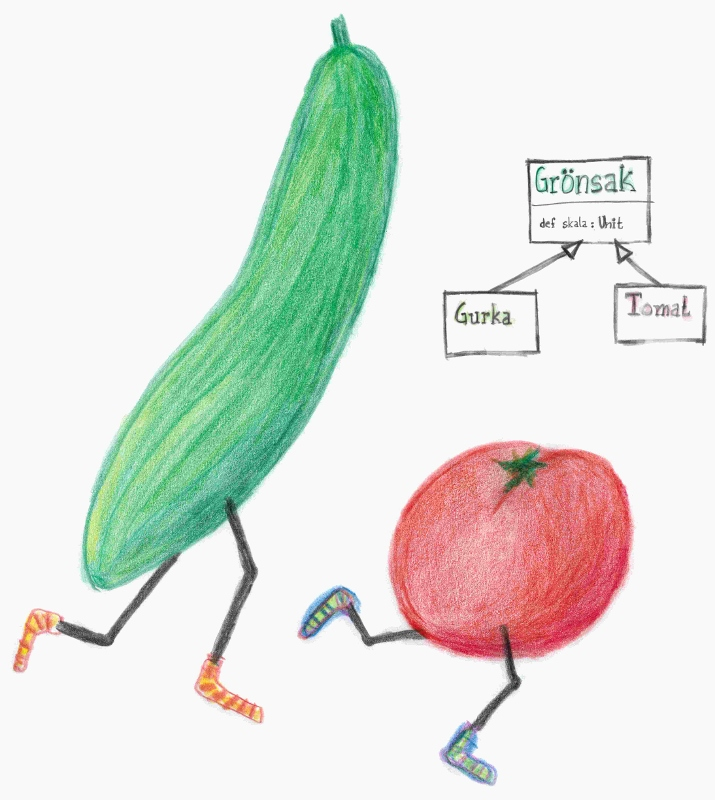
\includegraphics[width=1.5\textwidth]{../img/gurka-tomat-715x800}
\end{minipage}
\end{Slide}


\begin{Slide}{Varför behövs arv?}
\begin{itemize}
\item Man kan använda arv för att dela upp kod i:
\begin{itemize}
\item \Emph{generella} (gemensamma) delar och
\item \Emph{specifika} (specialanpassade) delar.
\end{itemize}

\item Man kan åstadkomma \Emph{kontrollerad flexibilitet}:
\begin{itemize}
\item Klientkod kan \Emph{utvidga} \Eng{extend} ett givet API med egna specifika tillägg.
\end{itemize}

\item Man kan använda arv för att deklarera en gemensam \Emph{bastyp} så att generiska samlingar kan ges en mer specifik elementtyp.
\begin{itemize}
\item Det räcker att man vet bastypen för att kunna anropa gemensamma metoder på alla element i samlingen.
\end{itemize}
\end{itemize}
\end{Slide}


\begin{Slide}{Behovet av gemensam bastyp}\SlideFontSmall
\begin{REPL}
scala> class Gurka(val vikt: Int)

scala> class Tomat(val vikt: Int)

scala> val gurkor = Vector(new Gurka(200), new Gurka(300))
gurkor: scala.collection.immutable.Vector[Gurka] =
  Vector(Gurka@60856961, Gurka@2fd953a6)

scala> gurkor.map(_.vikt)
res0: scala.collection.immutable.Vector[Int] = Vector(200, 300)

scala> val grönsaker = Vector(new Gurka(200), new Tomat(42))
grönsaker: scala.collection.immutable.Vector[Object] =
  Vector(Gurka@669253b7, Tomat@5305c37d)

scala> grönsaker.map(_.vikt)
<console>:15: error: value vikt is not a member of Object
       grönsaker.map(_.vikt)
\end{REPL}
Hur ordna en mer specifik typ än \code{Vector[Object]}? \pause$\rightarrow$ Skapa en \Emph{bastyp}!
\end{Slide}




\begin{Slide}{Skapa en gemensam bastyp}
Typen \textit{\textbf{\texttt{Grönsak}}} är en \Emph{bastyp} i nedan arvshierarki:

\vspace{1em}
\begin{center}
\newcommand{\TextBox}[1]{\raisebox{0pt}[1em][0.5em]{#1}}
\tikzstyle{umlclass}=[rectangle, draw=black,  thick, anchor=north, text width=2cm, rectangle split, rectangle split parts = 3]
\begin{tikzpicture}[inner sep=0.5em]
\node [umlclass, rectangle split parts = 1, xshift=0cm] (BaseType)  {
            \textit{\textbf{\centerline{\TextBox{\code{Grönsak}}}}}
            %\nodepart[]{second}\TextBox{\code{val vikt: Int}}
        };

\node [umlclass, rectangle split parts = 1]  at (2cm,-2cm) (SubType1) {
            \textbf{\centerline{\TextBox{\code{Gurka}}}}
            %\nodepart[]{second} \TextBox{~}
        };

\node [umlclass, rectangle split parts = 1] at (-2cm,-2cm) (SubType2)  {
            \textbf{\centerline{\TextBox{\code{Tomat}}}}
            %\nodepart[]{second} \TextBox{talk(): void}
        };
\draw[umlarrow] (SubType1.north) -- ++(0,0.5) -| (BaseType.south);
\draw[umlarrow] (SubType2.north) -- ++(0,0.5) -| (BaseType.south);
\end{tikzpicture}

\pause
\vspace{2em} Pilen ~ \tikz\draw[umlarrow] (0,0) -- (0,0.5); ~ betecknar \Emph{arv} och utläses ''\Alert{är en}''

\pause
{\vspace{1em}\SlideFontSmall Typerna \code{Tomat} och \code{Gurka} är \Emph{subtyper} till den \Emph{abstrakta} typen \code{Grönsak}.}
\end{center}
\end{Slide}







\begin{Slide}{Skapa en gemensam bastyp med \texttt{trait} och \texttt{extends}}\SlideFontSmall
Med \code{trait Grönsak} kan klasserna \code{Gurka} och \code{Tomat} få en gemensam \Emph{bastyp} genom att båda \Emph{subtyperna} gör \code{extends Grönsak}:
\begin{REPL}
scala> trait Grönsak

scala> class Gurka(val vikt: Int) extends Grönsak

scala> class Tomat(val vikt: Int) extends Grönsak

scala> val grönsaker = Vector(new Gurka(200), new Tomat(42))
grönsaker: scala.collection.immutable.Vector[Grönsak] =
  Vector(Gurka@3dc4ed6f, Tomat@2823b7c5)


\end{REPL}
\pause
Men det är fortfarande inte som vi vill ha det:
\begin{REPLnonum}
scala> grönsaker.map(_.vikt)
<console>:15: error: value vikt is not a member of Grönsak
       grönsaker.map(_.vikt)
\end{REPLnonum}
\end{Slide}



\begin{Slide}{En gemensam bastyp med gemensamma delar}\SlideFontSmall
Placera gemensamma medlemmar i bastypen:

\vspace{1em}
\begin{center}
\newcommand{\TextBox}[1]{\raisebox{0pt}[1em][0.5em]{#1}}
\tikzstyle{umlclass}=[rectangle, draw=black,  thick, anchor=north, text width=3cm, rectangle split, rectangle split parts = 3]
\begin{tikzpicture}[inner sep=0.5em]
\node [umlclass, rectangle split parts = 2, xshift=0cm] (BaseType)  {
            \textit{\textbf{\centerline{\TextBox{\code{Grönsak}}}}}
            \nodepart[]{second}\TextBox{\code{val vikt: Int}}
        };

\node [umlclass, rectangle split parts = 1]  at (2cm,-3cm) (SubType1) {
            \textbf{\centerline{\TextBox{\code{Gurka}}}}
            %\nodepart[]{second} \TextBox{~}
        };

\node [umlclass, rectangle split parts = 1] at (-2cm,-3cm) (SubType2)  {
            \textbf{\centerline{\TextBox{\code{Tomat}}}}
            %\nodepart[]{second} \TextBox{talk(): void}
        };
\draw[umlarrow] (SubType1.north) -- ++(0,0.5) -| (BaseType.south);
\draw[umlarrow] (SubType2.north) -- ++(0,0.5) -| (BaseType.south);
\end{tikzpicture}
\end{center}
\vspace{2em}
\begin{itemize}
\item Alla grönsaker har attributet \code{val vikt}.
\item Det specifika värdet på vikten definieras \Alert{inte} i bastypen.
\item Medlemen \code{vikt} kallas  \Emph{abstrakt} eftersom den \Alert{saknar implementation}.
\end{itemize}
\end{Slide}





\begin{Slide}{Placera gemensamma delar i bastypen}

Vi inkluderar det gemensamma attributet \code{val vikt} som en \Emph{abstrakt medlem} i bastypen:

\begin{Code}
trait Grönsak { val vikt: Int }

class Gurka(val vikt: Int) extends Grönsak

class Tomat(val vikt: Int) extends Grönsak
\end{Code}
Nu vet kompilatorn att alla grönsaker har en vikt:
\begin{REPL}
scala> val grönsaker = Vector(new Gurka(200), new Tomat(42))
grönsaker: scala.collection.immutable.Vector[Grönsak] =
  Vector(Gurka@3dc4ed6f, Tomat@2823b7c5)

scala> grönsaker.map(_.vikt)
res0: scala.collection.immutable.Vector[Int] = Vector(200, 42)
\end{REPL}

\end{Slide}





\begin{Slide}{Scalas typhierarki och typen \texttt{Object}}
Den översta delen av typhierarkin i Scala:
\vspace{1em}
\begin{center}
\newcommand{\TextBox}[1]{\raisebox{0pt}[1em][0.5em]{#1}}
\tikzstyle{umlclass}=[rectangle, draw=black,  thick, anchor=north, text width=2.5cm, rectangle split, rectangle split parts = 3]
\begin{tikzpicture}[inner sep=0.5em]
\node [umlclass, rectangle split parts = 1, xshift=0cm] (BaseType)  {
            \textit{\textbf{\centerline{\TextBox{\code{Any}}}}}
            %\nodepart[]{second}\TextBox{\code{def toString: String}}
        };

\node [umlclass, rectangle split parts = 1]  at (2cm,-2cm) (SubType1) {
            \textit{\textbf{\centerline{\TextBox{\code{AnyRef}}}}}
            %\nodepart[]{second} \TextBox{~}
        };

\node [umlclass, rectangle split parts = 1] at (-2cm,-2cm) (SubType2)  {
            \textit{\textbf{\centerline{\TextBox{\code{AnyVal}}}}}
            %\nodepart[]{second} \TextBox{talk(): void}
        };
\draw[umlarrow] (SubType1.north) -- ++(0,0.5) -| (BaseType.south);
\draw[umlarrow] (SubType2.north) -- ++(0,0.5) -| (BaseType.south);
\end{tikzpicture}
\end{center}
\begin{itemize}\SlideFontSmall
\item De numeriska typerna \code{Int}, \code{Double}, etc är subtyper till \Emph{\code{AnyVal}} och kallas \Emph{värdetyper} och lagras på ett speciellt, effektivt sätt i minnet.
\item Alla dina egna klasser är subtyper till \Emph{\texttt{AnyRef}} och kallas \Emph{referenstyper} och kräver (direkt eller indirekt) konstruktion med \code{new}.
\item \texttt{AnyRef} motsvaras av \Alert{\code{java.lang.Object}} i JVM.
\end{itemize}
\end{Slide}



\begin{Slide}{Implicita supertyper till dina egna klasser}
Alla dina egna typer ingår underförstått i Scalas typhierarki:

\vspace{1em}
\begin{center}
\newcommand{\TextBox}[1]{\raisebox{0pt}[1em][0.5em]{#1}}
\tikzstyle{umlclass}=[rectangle, draw=black,  thick, anchor=north, text width=2cm, rectangle split, rectangle split parts = 3]
\begin{tikzpicture}[inner sep=0.5em, scale=0.8, every node/.style={scale=0.8}]
\node [umlclass, rectangle split parts = 1, xshift=0cm] at (0,-0.3cm)(BaseType)  {
            \textit{\textbf{\centerline{\TextBox{\code{Any}}}}}
            %\nodepart[]{second}\TextBox{\code{def toString: String}}
        };

\node [umlclass, rectangle split parts = 1]  at (2cm,-2cm) (SubType1) {
            \textit{\textbf{\centerline{\TextBox{\code{AnyRef}}}}}
            %\nodepart[]{second} \TextBox{~}
        };

\node [umlclass, rectangle split parts = 1] at (-2cm,-2cm) (SubType2)  {
            \textit{\textbf{\centerline{\TextBox{\code{AnyVal}}}}}
            %\nodepart[]{second} \TextBox{talk(): void}
        };


\node [umlclass, rectangle split parts = 1] at (2cm,-3.5cm) (SubSubType)  {
            \textit{\textbf{\centerline{\TextBox{\code{Grönsak}}}}}
            %\nodepart[]{second} \TextBox{talk(): void}
        };

\node [umlclass, rectangle split parts = 1] at (3.5cm,-5.25cm) (SubSubSubType1)  {
            \textbf{\centerline{\TextBox{\code{Gurka}}}}
            %\nodepart[]{second} \TextBox{talk(): void}
        };

\node [umlclass, rectangle split parts = 1] at (0.5cm,-5.25cm) (SubSubSubType2)  {
            \textbf{\centerline{\TextBox{\code{Tomat}}}}
            %\nodepart[]{second} \TextBox{talk(): void}
        };


\draw[umlarrow] (SubType1.north) -- ++(0,0.3) -| (BaseType.south);
\draw[umlarrow] (SubType2.north) -- ++(0,0.3) -| (BaseType.south);
\draw[umlarrow] (SubSubType.north) -- (SubType1.south);
\draw[umlarrow] (SubSubSubType1.north) -- ++(0,0.3) -| (SubSubType.south);
\draw[umlarrow] (SubSubSubType2.north) -- ++(0,0.3) -| (SubSubType.south);
\end{tikzpicture}
\end{center}
\end{Slide}


\begin{Slide}{Vad är en trait?}
\begin{itemize}
\item \Alert{Trait} betyder \Emph{egenskap} på engelska.

\item En trait liknar en klass, \Alert{men} speciella regler gäller:

\begin{itemize}

\item den \Emph{kan} innehålla delar som \Emph{saknar implementation}

\item den \Emph{kan mixas} med flera andra traits så att olika koddelar kan återanvändas på flexibla sätt.

\item den \Alert{kan inte} instansieras direkt som den är.

\item den \Alert{kan inte} ha klassparametrar eller konstruktorer.
\end{itemize}

\pause
\item {\SlideFontSmall Jämförelse med Java:}
\begin{itemize}\SlideFontTiny
\item En Scala-trait liknar det som i Java kallas \jcode{interface}, men man kan göra mer med Scala-traits: färre begränsningar, fler abstraktionsmöjligheter.

\item En Scala-trait med enbart abstrakta medlemmar kompileras till bytekod i JVM:en som kan användas från Java-kod precis som ett Java-interface.
\end{itemize}
\end{itemize}

\end{Slide}

\begin{Slide}{Vad används en trait till?}
En \code{trait} används för att skapa en bastyp som kan vara hemvist för gemensamma delar hos subtyper:
\begin{Code}
trait Bastyp { val x = 42 }                 // Bastyp har medlemmen x
class Subtyp1 extends Bastyp { val y = 43 } // Subtyp1 ärver x, har även y
class Subtyp2 extends Bastyp { val z = 44 } // Subtyp2 ärver x, har även z
\end{Code}
\pause\vspace{-0.5em}
\begin{REPL}
scala> val a = new Subtyp1
a: Subtyp1 = Subtyp1@51016012

scala> a.x
res0: Int = 42

scala> a.y
res1: Int = 43

scala> a.z
<console>:15: error: value z is not a member of Subtyp1

scala> new Bastyp
<console>:13: error: trait Bastyp is abstract; cannot be instantiated
\end{REPL}

\end{Slide}


\begin{Slide}{En trait kan ha abstrakta medlemmar}
\begin{Code}
trait X { val x: Int }   // x är abstrakt, d.v.s. saknar implementation
class A extends X { val x = 42 }   // x ges en implementation
class B extends X { val x = 43 }   // x ges en annan implementation
\end{Code}
\pause\vspace{-0.5em}
\begin{REPL}
scala> val a = new A
a: A = A@5faeada1

scala> val b = new B
b: B = B@cb51256

scala> val xs = Vector(a,b)
xs: scala.collection.immutable.Vector[X] = Vector(A@5faeada1, B@cb51256)

scala> xs.map(_.x)
res0: scala.collection.immutable.Vector[Int] = Vector(42, 43)

scala> class Y { val y: Int }
  error: class Y needs to be abstract, since value y is not defined

scala> trait Z(x: Int)
  error: traits or objects may not have parameters

\end{REPL}
\end{Slide}


\begin{Slide}{Terminologi och nyckelord vid arv}\SlideFontTiny

\begin{tabular}{r  l}
\Emph{subtyp}           & en typ som ärver en supertyp\\
\Emph{supertyp}         & en typ som ärvs av en subtyp\\
\Emph{bastyp}           & en typ som är rot i ett arvsträd\\
\Emph{abstrakt medlem}  & en medlem som saknar implementation\\
\Emph{konkret medlem}   & en medlem som ej saknar implementation\\
\Emph{abstrakt typ}     & en typ som kan ha abstrakta medlemmar; kan ej instansieras\\
\Emph{konkret typ}      & en typ som ej har abstrakta medlemmar; kan instansieras\\
\code|class|            & en klass är en konkret typ: \Alert{kan ej ha abstrakta medlemmar}\\
\code|abstract class|   & en klass är en abstrakt typ som \Emph{kan ha parametrar}\\
\code|trait|            & är en abstrakt typ, \Alert{kan ej ha parametrar} men \Emph{kan mixas in}\\
\code|extends|          & står före en supertyp, medför arv av supertypens medlemmar\\
\code|override|         & en medlem överskuggar (byter ut) en medlem i en superttyp\\
\code|protected|        & gör en medlem synlig i subtyper till denna typ (jmf \code|private|)\\
\code|final gurka|      & gör medlemen gurka final: förhindrar överskuggning\\
\code|final class|      & gör klassen final: förhindrar vidare subtypning\\
\code|sealed trait|     & förseglad trait: bara de direkta subtyperna i denna kodfil\\
\code|super.gurka|      & refererar till supertypens medlem \code|gurka| (jmf \code|this|)\\
\end{tabular}

\ifkompendium\else
\pause
\begin{tikzpicture}[overlay]
     \node at (10.7,0.6) {
\includegraphics[scale=0.36]{../img/ttsuper}};
\end{tikzpicture}
\fi

\end{Slide}


\begin{Slide}{Abstrakta och konkreta medlemmar}
\vspace{-0.5em}\scalainputlisting[numbers=left,numberstyle=,basicstyle=\fontsize{6}{7}\ttfamily\selectfont]{../compendium/examples/workspace/w07-inherit/src/vego1.scala}
\end{Slide}


\begin{Slide}{Undvika kodduplicering med hjälp av arv}
\scalainputlisting[numbers=left,numberstyle=,basicstyle=\fontsize{6}{7.3}\ttfamily\selectfont]{../compendium/examples/workspace/w07-inherit/src/vego2.scala}
\end{Slide}




\begin{Slide}{Varför kan kodduplicering orsaka problem?}
\begin{itemize}
\item Mer att skriva (inte jättestort problem)
\pause
\item Fler kodrader att läsa och förstå
\pause
\item Fler kodrader som påverkas vid tillägg
\pause

\item Fler kodrader att underhålla:
\begin{itemize}
\item Om man rättar en bug på ett ställe måste man komma ihåg att göra \Alert{exakt samma ändring} på alla de ställen där kodduplicering förekommer $\rightarrow$ \Alert{risk för nya buggar}
\end{itemize}

\pause

\item Principen på engelska: \code{ DRY == "Don't Repeat Yourself!"}

\pause

\item {Men det kan finnas tillfällen när kodduplicering faktiskt är att föredra: t.ex. om man vill att olika delar av koden ska vara helt oberoende av varandra.}
\end{itemize}
\end{Slide}




\begin{Slide}{Överskuggning}
\vspace{-0.5em}\scalainputlisting[numbers=left,numberstyle=,basicstyle=\fontsize{6}{7.3}\ttfamily\selectfont]{../compendium/examples/workspace/w07-inherit/src/vego3.scala}
\end{Slide}

\begin{Slide}{En final medlem kan ej överskuggas}
\vspace{-0.5em}\scalainputlisting[numbers=left,numberstyle=,basicstyle=\fontsize{6}{7.3}\ttfamily\selectfont]{../compendium/examples/workspace/w07-inherit/src/vego4.scala}
\end{Slide}


\begin{Slide}{Protected ger synlighet begränsad till subtyper}
\begin{REPL}
scala> trait Super {
         private val minHemlis = 42
         protected val vårHemlis = 42
       }

scala> class Sub extends Super { def avslöjad = minHemlis }
error: not found: value minHemlis

scala> class Sub extends Super { def avslöjad = vårHemlis }

scala> val s = new Sub
s: Sub = Sub@2eee9593

scala> s.avslöjad
res0: Int = 42

scala> s.minHemlis
error: value minHemlis is not a member of Sub

scala> s.vårHemlis
error: Access to protected value vårHemlis not permitted
\end{REPL}
\end{Slide}


\begin{Slide}{Filnamnsregler och -konventioner}
\begin{itemize}
\item Java
\begin{itemize}
\item I Java får man bara ha \Alert{en enda} publik klass per kodfil.
\item I Java måste kodfilen ha \Alert{samma namn} som den publika klassen, t.ex. \code{KlassensNamn.java}
\end{itemize}
\item Scala
\begin{itemize}
\item I Scala får man ha \Emph{många} klasser/traits/singelobjekt i samma kodfil.
\item I Scala får man döpa kodfilerna \Emph{oberoende} av deras innehåll. \pause Dessa \Emph{konventioner} används:
\begin{itemize}
\item Om en kodfil bara innehåller \Emph{en enda} klass/trait/singelobjekt ge filen samma namn som innehållet, t.ex. \code{KlassensNamn.scala}
\item Om en kodfil innehåller \Emph{flera} saker, döp filen till något som återspeglar hela innehållet och använd \Emph{liten begynnelsebokstav}, t.ex. \code{drawing.scala} eller \code{bastypensNamn.scala}
\end{itemize}


\end{itemize}

\end{itemize}
\end{Slide}


\begin{Slide}{Klasser, arv och klassparametrar}\SlideFontTiny
Klasser kan ärva klasser. Om superklassen har klassparametrar måste primärkonstruktor ges argument efter \code{extends}.

\scalainputlisting[numbers=left,numberstyle=,basicstyle=\fontsize{6.4}{7.7}\ttfamily\selectfont]{../compendium/examples/workspace/w07-inherit/src/personExample1.scala}

\end{Slide}


\begin{Slide}{Statisk och dynamisk typ}\SlideFontSmall
\begin{Code}
    var p: Person = new Forskare("Robin Smith", "Lund", "Professor Dr")
\end{Code}
\begin{itemize}
\item Den \Emph{statiska typen} för \code{p} är \code{Person} vilket gör att vi sedan kan låta \code{p} referera till andra instanser som är av typen Person.
\begin{Code}
p = new Student("Kim Robinson", "Lund", "Data")
\end{Code}

\pause

\item Med ''statisk typ'' menas den typinformation som kompilatorn känner till vid kompileringstid.

\pause
\item Den \Emph{dynamiska typen}, även kallad \Emph{körtidstypen}, som gäller under körning är här mer specifik och mångfaceterad: \code{p} är efter tilldelning nu Student, Person och Akademiker (men inte Examinerad).

\pause

\item Man kan undersöka om den dynamiska typen för \code{p} är \code{EnVissTyp} med  \code{p.isInstanceOf[EnVissTyp]}

\pause

\item Man kan säga åt kompilatorn: \emph{''jag garanterar att p är av typen \code{EnVissTyp} så du kan omforma den till \code{EnVissTyp}''} med  \code{p.asInstanceOf[EnVissTyp]} \\ \pause (detta är inte så vanligt i normal Scala-kod)
\end{itemize}
\end{Slide}




\begin{Slide}{Inmixning}\SlideFontTiny
Man kan ärva flera traits. Detta kallas inmixning \Eng{mix-in} och görs med \code{with}.
\scalainputlisting[numbers=left,numberstyle=,basicstyle=\fontsize{6.4}{7.7}\ttfamily\selectfont]{../compendium/examples/workspace/w07-inherit/src/personExample2.scala}
\end{Slide}



\begin{Slide}{\texttt{isInstanceOf} och \texttt{asInstanceOf}}\SlideFontTiny
Testa körtidstyp med \code{isInstanceOf[Typ]}. Lova kompilatorn (och ta själv ansvar för) att det är en viss körtidstyp med \code{asInstanceOf[Typ]}. OBS! Använd hellre \code{match}.
\scalainputlisting[basicstyle=\small\SlideFontSize{6.2}{7.6}\ttfamily\selectfont]{../compendium/examples/workspace/w07-inherit/src/personExample3.scala}
\end{Slide}



\begin{Slide}{Polymorfism och dynamisk bindning}\SlideFontTiny
\begin{Code}[basicstyle=\SlideFontSize{6.2}{7.5}\ttfamily\selectfont]
trait Robot { def work(): Unit }

case class CleaningBot(name: String) extends Robot {
  override def work(): Unit = println(" Städa Städa")
}

case class TalkingBot(name: String) extends Robot {
  override def work(): Unit = println(" Prata Prata")
}
\end{Code}
\Emph{Polymorfism} betyder ''många former''. Referenserna r och bot nedan kan ha olika ''former'', d.v.s de kan referera till olika sorters robotar. \\ \Emph{Dynamisk bindning} innebär att körtidstypen avgör vilken metod som körs.
\begin{REPL}[numbers=left, basicstyle=\color{white}\SlideFontSize{6.2}{7.5}\ttfamily\selectfont]
scala> def robotDoWork(bot: Robot) = { print(bot); bot.work }

scala> var r: Robot = new CleaningBot("Wall-E")

scala> robotDoWork(r)
CleaningBot(Wall-E) Städa Städa

scala> r = new TalkingBot("C3PO")

scala> robotDoWork(r)
TalkingBot(C3PO) Prata Prata
\end{REPL}
\end{Slide}


\begin{Slide}{Anonym klass}
Om man har en abstrakt typ med saknade implementationer kan man fylla i det som fattas i dessa i ett extra block som ''hängs på'' vid instansiering:
\begin{REPL}
scala> trait Grönsak { val vikt: Int }
defined trait Grönsak

scala> new Grönsak
<console>:13: error: trait Grönsak is abstract; cannot be instantiated
       new Grönsak
       ^

scala> new Grönsak { val vikt = 42 }
res0: Grönsak = $anon$1@4e3f2908
\end{REPL}
Man får då vad som kallas en \Emph{anonym klass}. (I detta fall en ganska konstig grönsak som inte är någon speciell sorts grönsak med som ändå har en vikt.)
\end{Slide}


\Subsection{Uppräknade värden}


\begin{Slide}{Uppräknade värden med heltal}\SlideFontSmall
Vi kan använda heltalskonstanter för att representera olika färger.
\begin{Code}
object Färg {
  val Spader = 1
  val Hjärter = 2
  val Ruter = 3
  val Klöver = 4
}
\end{Code}
\begin{Code}[language=,keywords={case,class}]
case class Kort(färg: Int, valör: Int)
\end{Code}

Vi kan nu använda våra uppräknade färgvärden så här:
\begin{REPLnonum}
scala> import Färg._
scala> Kort(Ruter, 7)
\end{REPLnonum}
\pause Men kompilatorn \Alert{kan inte hindra} denna bugg:
\begin{REPLnonum}
scala> Kort(42, 7)
\end{REPLnonum}

\end{Slide}


\begin{Slide}{Uppräknade värden med case-objekt}\SlideFontSmall
Vi kan använda case-objekt för att representera olika färger.
\begin{Code}[language=,keywords={sealed,trait,object,case,class,extends}]
sealed trait Färg
case object Spader  extends Färg
case object Hjärter extends Färg
case object Ruter   extends Färg
case object Klöver  extends Färg

case class Kort(färg: Färg, valör: Int)
\end{Code}

Vi kan nu använda våra uppräknade färgvärden så här:
\begin{REPL}
scala> Kort(Ruter, 7)

scala> Kort(Spader, 1)
\end{REPL}
\begin{itemize}
\item Kompilatorn \Emph{garanterar} att vi bara använder exakt dessa färger.

\item Nyckelordet \code{sealed} förhindrar fler subtyper förutom de som finns här.

\item \code{case} före \code{object} ger en najs \code{toString} och möjliggör matchning \\
(mer om matchning i w10).

\end{itemize}

\end{Slide}

\begin{Slide}{Uppräknade värden i samling}\SlideFontSmall
Vi kan placera case-objekten i en samling som kan användas i loopar. \\ Ett lämpligt ställe för en sådan samling är i kompanjonsobjektet till \code{Färg}.
\begin{Code}
sealed trait Färg
object Färg {
  val values = Vector(Spader, Hjärter, Ruter, Klöver)
}
case object Spader extends Färg
case object Hjärter extends Färg
case object Ruter extends Färg
case object Klöver extends Färg
\end{Code}

\begin{REPL}
scala> val allaEss = for (f <- Färg.values) yield Kort(f, 1)
\end{REPL}
\end{Slide}


\begin{Slide}{Uppräknade värden med heltalsomvandling}\SlideFontSmall
Med en \code{sealed abstract class} och ett heltalsattrribut \code{toInt} som klassparameter kan vi erbjuda omvandling till heltal.
\begin{Code}
sealed abstract class Färg(final val toInt: Int)
object Färg {
  val values = Vector(Spader, Hjärter, Ruter, Klöver)
}
case object Spader  extends Färg(0)
case object Hjärter extends Färg(1)
case object Ruter   extends Färg(2)
case object Klöver  extends Färg(3)
\end{Code}

\begin{REPL}
scala> Kort(Ruter, 1).färg.toInt
res0: Int = 2
\end{REPL}
Nyckelordet \code{abstract} förhindrar instansiering av \code{Färg}. \\
Nyckelordet \code{final} förhindrar överskuggning av attributet \code{toInt}. \\
Nyckelordet \code{sealed} förhindrar vidare subtypning av \code{Färg}.
\end{Slide}



\Subsection{Exempel: Shape}


\begin{Slide}{Exempel: shapes1.scala}
Typisk Scala-kod: En trait som bastyp åt flera case-klasser.
\scalainputlisting[numbers=left,numberstyle=,basicstyle=\fontsize{6.4}{7.7}\ttfamily\selectfont]{../compendium/examples/workspace/w07-inherit/src/shapes1.scala}
\end{Slide}

\begin{Slide}{Exempel: shapesTest1.scala}
Test av konkreta subklasser till bastypen \code{Shape}.
\scalainputlisting[numbers=left,numberstyle=,basicstyle=\fontsize{6.4}{7.7}\ttfamily\selectfont]{../compendium/examples/workspace/w07-inherit/src/shapesTest1.scala}

\begin{REPL}
Rectangle((100.0,100.0),(75.0,120.0))
Rectangle((141.0,183.0),(75.0,120.0))
Triangle((0.0,0.0),(4.0,0.0),(4.0,3.0))
Triangle((1.0,1.0),(4.0,0.0),(4.0,3.0))
Triangle((0.0,0.0),(4.0,0.0),(4.0,3.0))
\end{REPL}
\end{Slide}


\begin{Slide}{Fördjupningsexempel gränssnitt: draw.scala}
Två traits som kan användas för att ''koppla ihop'' kod och ge flexibilitet i implementationen:
\scalainputlisting[%numbers=left,numberstyle=,
basicstyle=\fontsize{9}{11}\ttfamily\selectfont]{../compendium/examples/workspace/w07-inherit/src/draw.scala}

\pause
\setlength{\leftmargini}{0pt}
\begin{itemize}\SlideFontSmall
\item  Traits som använda för att abstrahera implementation och möjliggöra uppfyllandet av ett slags ''kontrakt'' om vad som ska finnas kallas \Emph{gränssnitt} \Eng{interface} och används ofta för att skapa av ett flexibelt api.

%\item Implementationen av de delar vi vill kunna ändra senare placeras i subtyper som inte används direkt av klientkoden. 

\item Vi visar bara information om vad som erbjuds men inte hur det ser ut ''inuti''.

\end{itemize}
\end{Slide}

\begin{Slide}{Exempel: shapes2.scala}\SlideFontTiny
Genom att \Emph{mixa in} vår \code{trait CanDraw} kan en rektangel nu även ritas ut:

\scalainputlisting[numbers=left,numberstyle=,basicstyle=\fontsize{6.5}{7.8}\ttfamily\selectfont]{../compendium/examples/workspace/w07-inherit/src/shapes2.scala}

\pause
\vspace{-0.5em}Notera: ingen ändring i \code {Shape}! Vi behöver nu bara ett \Emph{\code{DrawingWindow}}...
\end{Slide}


\begin{Slide}{Exempel: SimpleDrawingWindow.scala}\SlideFontTiny
\vspace{-0.35em}
Vi skapar en ny klass som ärver \code{SimpleWindow}, som \Alert{dessutom} även \Emph{är ett} \code{DrawingWindow}, tack vare \Emph{inmixning} med nyckelordet \code{with}.\\
Observera att vi måste skicka vidare klassparametrarna till superklassens konstruktor.

\scalainputlisting[numbers=left,numberstyle=,basicstyle=\fontsize{6.4}{7.7}\ttfamily\selectfont]{../compendium/examples/workspace/w07-inherit/src/SimpleDrawingWindow.scala}

\pause
\vspace{-0.35em}
\scalainputlisting[numbers=left,numberstyle=,basicstyle=\fontsize{6.4}{7.7}\ttfamily\selectfont]{../compendium/examples/workspace/w07-inherit/src/shapesTest2.scala}
\end{Slide}


%\begin{Slide}{Exempel: Robot}
%\begin{center}
%\newcommand{\TextBox}[1]{\raisebox{0pt}[1em][0.5em]{#1}}
%\begin{tikzpicture}[inner sep=0.5em]
%\node [umlclass, rectangle split parts = 2, xshift=0cm] (AbstractRobot)  {
%            \textit{\textbf{\centerline{\TextBox{AbstractRobot}}}}
%            \nodepart[]{second}\TextBox{work(): void}
%        };
%
%\node [umlclass, rectangle split parts = 2]  at (2cm,-3cm) (MuteRobot) {
%            \textbf{\centerline{\TextBox{MuteRobot}}}
%            \nodepart[]{second} \TextBox{~}
%        };
%
%\node [umlclass, rectangle split parts = 2] at (-2cm,-3cm) (TalkingRobot)  {
%            \textbf{\centerline{\TextBox{TalkingRobot}}}
%            \nodepart[]{second} \TextBox{talk(): void}
%        };
%\draw[umlarrow] (TalkingRobot.north) -- ++(0,0.5) -| (AbstractRobot.south);
%\draw[umlarrow] (MuteRobot.north) -- ++(0,0.5) -| (AbstractRobot.south);
%\end{tikzpicture}
%\end{center}
%\end{Slide}






\begin{Slide}{Attribut och metoder i UML-diagram}
\begin{center}
\begin{tikzpicture}
\node (Class) [umlclass, rectangle split parts = 3, xshift = -2cm, yshift=-1.5cm, text width = 4.2cm, scale=0.8]  {
            \textbf{\centerline{Name}}
            \nodepart[]{second}attr1: Type \newline attr2: Type
            \nodepart[]{third}method1(a: Type): Type \newline  method2(b: Type): Type
       };
\node (explain1)[above of = Class, yshift=1cm, text width=4.9cm]{En klass i ett \Emph{UML}-diagram kan ha 3 delar:};
\node (explain2)[below of = Class, yshift=-1cm]{Ibland utelämnar man typerna.};



\node [umlclass, rectangle split parts = 3]  at (4,0) (Robot) {
            \textbf{\centerline{Robot}}
            \nodepart[]{second}name: String
            \nodepart[]{third}work(): Unit
       };
\node [umlclass, rectangle split parts = 3]  at (4, -3) (TalkingRobot)  {
            \textbf{\centerline{TalkingRobot}}
            \nodepart[]{second} phrase: String
            \nodepart[]{third}speak(): Unit
        };
\draw[umlarrow] (TalkingRobot.north) -- ++(0,0.8) -| (Robot.south);
\end{tikzpicture}
\end{center}
\hskip2em\href{https://en.wikipedia.org/wiki/Class_diagram}{\SlideFontTiny en.wikipedia.org/wiki/Class\_diagram}
\end{Slide}

%!TEX encoding = UTF-8 Unicode
%!TEX root = ../lect-w09.tex

%%%


%\begin{Slide}{TODO: Begrepp att förklara}
%  Tänk igenom ordningen:
%  \begin{itemize}
%    \item OO, arv, supertyp, subtyp, bastyp, polymorfism, ... 
%  \end{itemize}
%\end{Slide}


\Subsection{Överskuggingsregler}

\begin{Slide}{Medlemmar, arv och överskuggning}\SlideFontTiny
\begin{multicols}{2}
Olika sorters överskuggningsbara medlemmar i klasser och traits i \Emph{Scala}:
\begin{itemize}
\item \code{def}
\item \code{val}
\item \code{lazy val}
\item \code{var}
\end{itemize}


\columnbreak

\pause

Olika sorters överskuggningsbara instansmedlemmar i \Emph{Java}:
\begin{itemize}
\item variabel 
\item metod
\end{itemize}

{\SlideFontTiny Medlemmar som är \jcode{static} kan ej överskuggas (men döljas) vid arv.}

\vspace{0.5em}
\end{multicols}

\pause
\begin{itemize}\SlideFontTiny
\item När man överskuggar \Eng{override} en medlemmen med en annan medlem med samma namn i en subtyp, får denna medlem en (ny) implementation. 

\item När man konstruerar ett objektorienterat språk gäller det att man definierar sunda överskuggningsregler vid arv. Detta är förvånansvärt knepigt.

\item Singelobjekt kan ej ärvas (och medlemmar i singelobjekt kan därmed ej överskuggas).
\end{itemize}
\end{Slide}


\begin{Slide}{Fördjupning: Regler för överskuggning i Scala} \SlideFontTiny
\label{slideW07:overriderules}
En medlem M1 i en supertyp får överskuggas av en medlem M2 i en subtyp, enligt dessa regler:
\begin{enumerate}
\item M1 och M2 ska ha samma namn och typerna ska matcha.
\item \code{def} får bytas ut mot: \code{def}, \code{val}, \code{var}, \code{lazy val}
\item \code{val} får bytas ut mot: \code{val}, och om M1 är abstrakt mot en \code{lazy val}.
\item \code{var} får bara bytas ut mot en \code{var}.
\item \code{lazy val} får bara bytas ut mot en \code{lazy val}.
\item Om en medlem i en supertyp är abstrakt \emph{behöver} man inte använda nyckelordet \code{override} i subtypen. (Men det är bra att göra det ändå så att kompilatorn hjälper dig att kolla att du verkligen överskuggar något.) 
\item Om en medlem i en supertyp är konkret \emph{måste} man använda nyckelordet \code{override} i subtypen, annars ges kompileringsfel.
\item M1 får inte vara \code{final}.
\item M1 får inte vara \code{private} eller \code{private[this]}, men kan vara \code{private[X]} om M2 också är \code{private[X]}, eller \code{private[Y]} om X innehåller Y.   
\item Om M1 är \code{protected} måste även M2 vara det.

\end{enumerate}
\end{Slide}


\begin{Slide}{Fördjupning: Regler för överskuggning i Java}
\url{http://docs.oracle.com/javase/tutorial/java/IandI/override.html}
\end{Slide}


\Subsection{\texttt{super}}

\begin{Slide}{Att skilja på mitt och ditt med \texttt{super}}
\begin{REPL}
scala> class X { val gurka = "super pepinos" }

scala> class Y extends X { 
         override val gurka = ":("
         val sg = super.gurka 
       }

scala> val y = new Y
y: Y = Y@26ba2a48

scala> y.gurka
res0: String = :(
\end{REPL}
Super Pepinos to the rescue:
\pause
\begin{REPLnonum}
scala> y.sg
res1: String = super pepinos

\end{REPLnonum}


\pause
\begin{tikzpicture}[overlay]
     \node at (7.5,1.7) {
\includegraphics[scale=0.5]{../img/ttsuper}};
\end{tikzpicture}
\href{http://www.pepinadas.com/tirassuper1.html}{\small www.pepinadas.com/tirassuper1.html}
\end{Slide}





\Subsection{Trait eller abstrakt klass?}

\begin{Slide}{Trait eller abstrakt klass?} 
\SlideFontSmall
\label{slideW07:traitorclass}
\begin{multicols}{2}
Använd en \Emph{trait} som supertyp om...
\begin{itemize}
\item ...du är osäker på vilket som är bäst. (Du kan alltid ändra till en abstrakt klass senare.)
\item ...du vill kunna mixa in din trait tillsammans med andra traits.
\item ...du bara har abstrakta medlemmar. 
\end{itemize}

\columnbreak

Använd en \Alert{abstrakt klass} som supertyp om...
\begin{itemize}
\item ...du vill ge supertypen en parameter vid konstruktion.
\item ...du vill ärva supertypen från klasser skrivna i Java.
\item ...du vill minimera vad som behöver omkompileras vid ändringar. 
\end{itemize}


\end{multicols}
\end{Slide}





%\begin{Slide}{Designexempel: Klassen ???}\small
%TODO:
%  \begin{itemize} 
%  \item 
%  \end{itemize}
%\end{Slide}











%!TEX encoding = UTF-8 Unicode
%!TEX root = ../lect-w09.tex

%%%

\ifkompendium\else


\Subsection{Veckans uppgifter}


\begin{Slide}{Övning: \texttt{inheritance}}
\begin{itemize}\SlideFontTiny
%!TEX encoding = UTF-8 Unicode

%!TEX root = ../compendium2.tex

\item Förstå följande begrepp: supertyp, subtyp, bastyp, abstrakt typ, polymorfism.
\item Kunna deklarera och använda en arvshierarki i flera nivåer med nyckelordet \code{extends}.
\item Kunna deklarera och använda inmixning med flera traits och nyckelordet \code{with}.
\item Kunna deklarera och känna till nyttan med finala klasser och finala attribut och nyckelordet \code{final}.
\item Känna till synlighetsregler vid arv och nyttan med privata och skyddade attribut.
\item Kunna deklarera och använda skyddade attribut med nyckelordet \code{protected}.
\item Känna till hur typtester och typkonvertering vid arv kan göras med metoderna \code{isInstanceOf} och \code{asInstanceOf} och känna till att detta görs bättre med \code{match}.
\item Känna till begreppet anonym klass.
\item Kunna deklarera och använda överskuggade metoder med nyckelordet \code{override}.
\item Känna till reglerna som gäller vid överskuggning av olika sorters medlemmar.
\item Kunna deklarera och använda hierarkier av klasser där konstruktorparametrar överförs till superklasser.
\item Kunna deklarera och använda uppräknade värden med case-objekt och gemensam bastyp.

\end{itemize}
\end{Slide}

\begin{Slide}{Instruktioner Grupplaboration}
\begin{itemize}\SlideFontSmall
%!TEX encoding = UTF-8 Unicode
%!TEX root = compendium.tex
\item 
Diskutera i din samarbetsgrupp hur ni ska dela upp koden mellan er i flera olika delar, som ni kan arbeta med var för sig. En sådan del kan vara en klass, en trait, ett objekt, ett paket, eller en funktion. 
\item
Varje del ska ha en \emph{huvudansvarig} individ. 
\item
Arbetsfördelningen ska vara någorlunda jämnt fördelad mellan gruppmedlemmarna.
\item
När ni redovisar er lösning ska ni börja med att redogöra för handledaren hur ni delat upp koden och vem som är huvudansvarig för vad. 
\item
Den som är huvudansvarig för en viss del redovisar den delen.
\item 
Grupplaborationer görs i huvudsak som hemuppgift. Salstiden används primärt för redovisning.
\end{itemize}
\end{Slide}

\begin{Slide}{Grupplaboration: \texttt{turtlerace-team}}
\begin{itemize}
%!TEX encoding = UTF-8 Unicode
%!TEX root = ../compendium2.tex

\item Kunna använda arv.
\item Kunna göra överskuggning av medlemmar i en supertyp med \code{override}.
\item Kunna referera till medlemmar i superklassen med \code{super} vid överskuggning.
\item Kunna förklara begreppet dynamisk bindning.

\end{itemize}
\end{Slide}



\fi


\Lecture{10}{Mönster, undantag}
%!TEX encoding = UTF-8 Unicode
%!TEX root = ../lect-week09.tex

%%%

\ifkompendium\else

\Subsection{Bonus}

\begin{Slide}{Grupper, antal medlemmar, bonus}
\begin{multicols}{2}
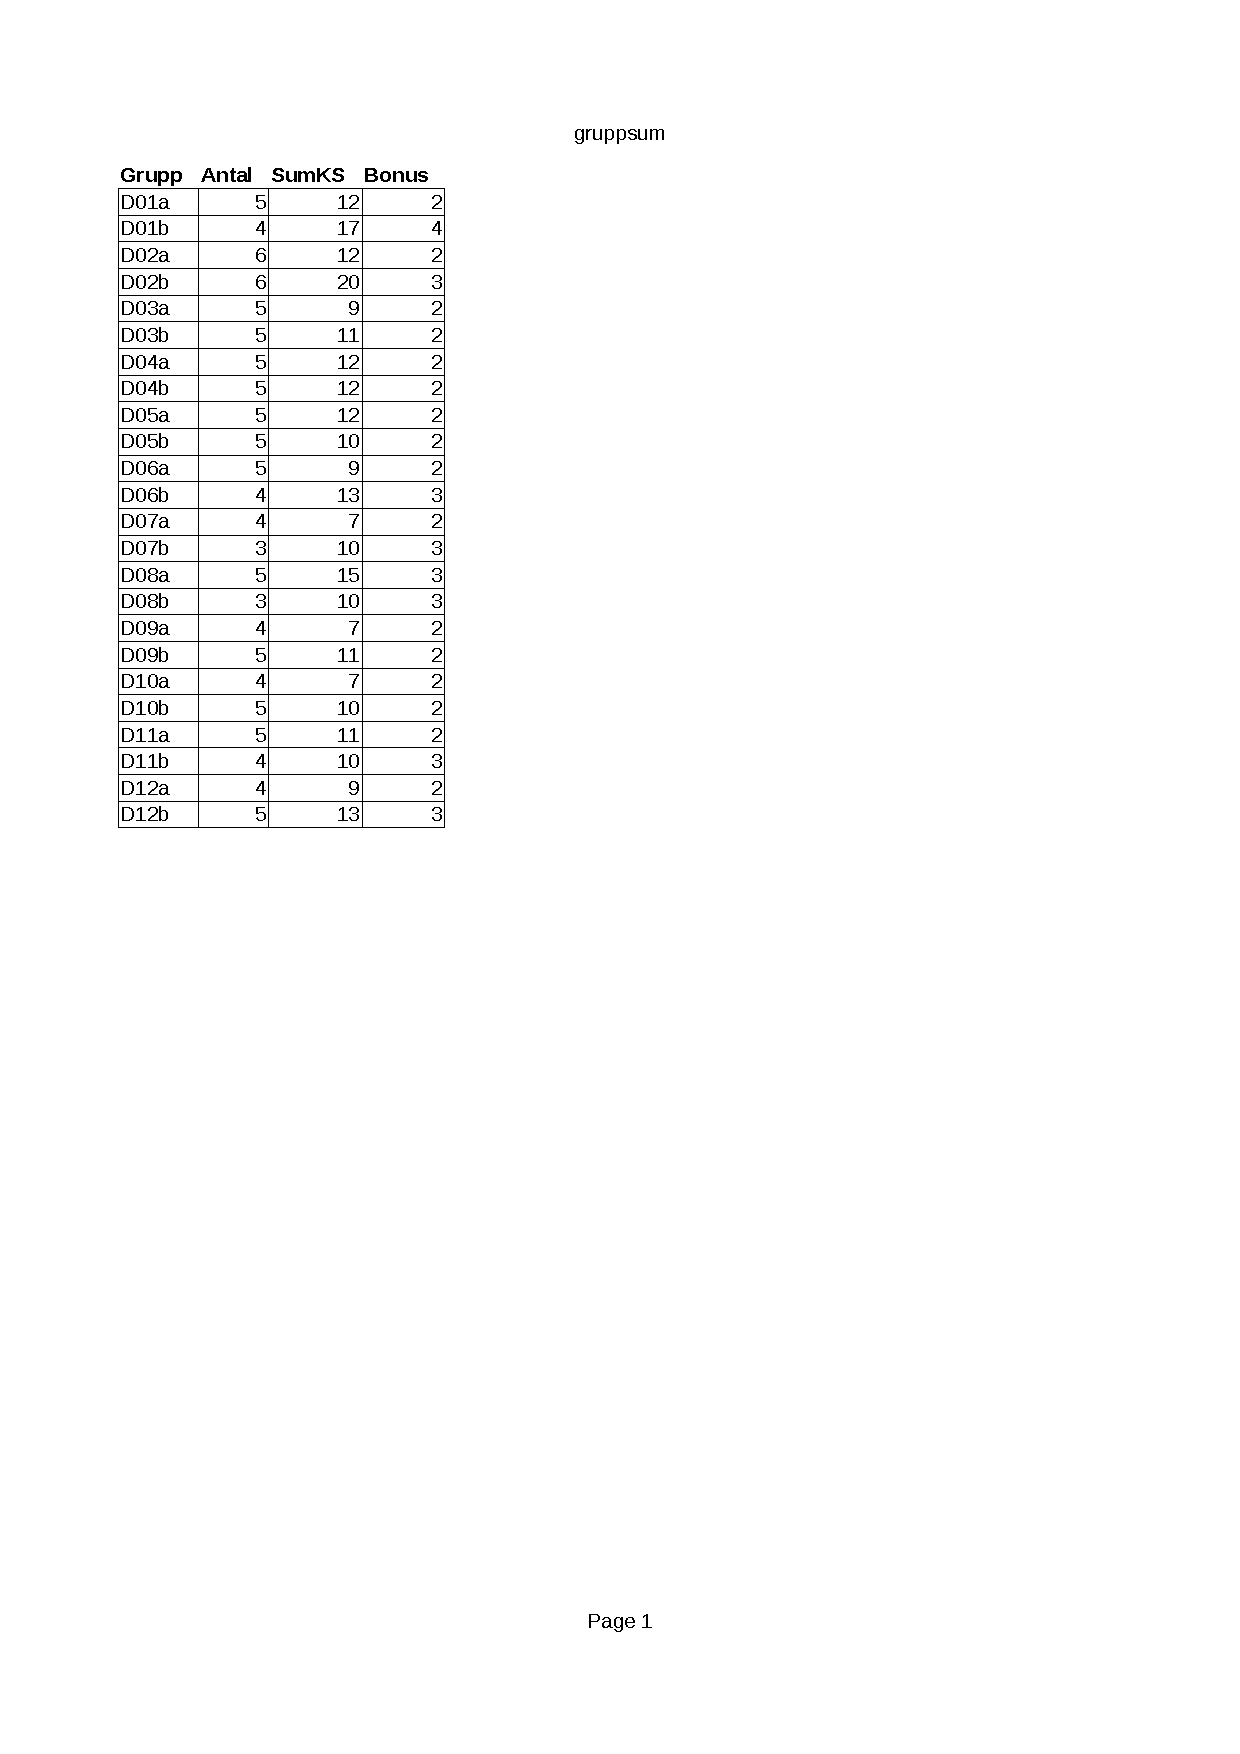
\includegraphics[clip, trim=0cm 1cm 3.2cm 2.5cm, width=0.9\textwidth]{../img/bonus-2016.pdf}

\columnbreak

\begin{itemize}
\pause
\item Bonus gäller vid första ordinarie tentatillfälle 
\pause
\item D07b och D08b har 3 st; \\ vill ni göra merge?

\end{itemize}
\end{multicols}
\end{Slide}

\Subsection{Specialundervisning}
\begin{Slide}{Specialundervisning}
Under vecka w09 och w10 (till att börja med) kommer vi att organisera \Emph{specialundervisning} under dessa \Alert{resurstider}:
\begin{itemize}
\item \Emph{Torsdag kl 8-10} i både \Alert{Falk} och \Alert{Val}  (Gustav, Valthor, Emil)
\item \Emph{Torsdag kl 10-12} i \Alert{Falk} (Maj)
\item OBS! Dessa rumtider är till för de som hade 0 eller 1 på kontrollskrivningen och som ansökt om specialundervisning via länk i speciell mejlinbjudan. 
\end{itemize}
\SlideFontSmall{Undantag: Om du har mer än 1 på kontrollskrivningen men inte alls har möjlighet att gå på någon annan resurstid än ovan är du också välkommen; anmäl då din situation till handledaren på plats och så får du vara med i gruppen och kan få svar på frågor etc. som vanligt.}
\end{Slide}
\fi












%!TEX encoding = UTF-8 Unicode
%!TEX root = ../lect-w10.tex

%%%


%\begin{Slide}{TODO: Begrepp att förklara}
%  Tänk igenom ordningen:
%  \begin{itemize}
%    \item java switch, scala match ... 
%  \end{itemize}
%\end{Slide}
%
%
%\begin{Slide}{Javas switch-sats}
%A switch in Java works with the byte, short, char, and int primitive data types. It also works with enumerated types (discussed in Enum Types), the String class, and a few special classes that wrap certain primitive types: Character, Byte, Short, and Integer
%\end{Slide}


\Subsection{Veckans lab: \texttt{chords-team}}
\begin{Slide}{Veckans lab: \texttt{chords-team}}\SlideFontSmall
Övergripande syfte:
\begin{itemize}
\item Träna på case-klasser, matchning, undantag
\item Jobba med ett större program med flera delar i olika filer
\item Jobba flera personer på samma program
\end{itemize}
Innehåll:
\begin{itemize}
\item Skapa och spara ackord på gitarr (6 strängar) och ukulele (4 strängar) 
\item Spela upp ackord med Javas inbyggda musikspelare inkapslad i \code{SimpleNotePlayer}
\item Rita ackord med \code{SimpleWindow} 
\end{itemize}
Hur mycket ni gör beror på hur många ni är i gruppen och hur stora ambitioner ni har. Diskutera detta med handledare på resurstid.
\end{Slide}

\begin{Slide}{Toner, oktaver och ackord}\SlideFontSmall
\begin{itemize}
\item Det finns 12 toner som har speciella namn: \\ C, C\#, D, D\#, etc. (uttalas: c, ciss, d, diss, etc.)
\item Jämför vita och svarta tangenter på ett piano: \\ avståndet mellan varje tangent är ett s.k. \emph{halvt tonsteg}. 
\item Toner återkommer i oktaver, modulo 12.
\item Tonen som representeras av strängen \code{"D2"} är tonen D i andra oktaven.
\item Tonen \code{"D2"} motsvarar heltalet \code{26} på labben.
\item Ett ackord består av flera toner.
\end{itemize}
\begin{REPL}[basicstyle=\color{white}\ttfamily\SlideFontSize{6}{7}\selectfont]
scala> val notes = Vector("C", "C#", "D", "D#", "E", "F", "F#", "G", "G#", "A", "A#", "B")

scala> notes.size
res0: Int = 12

scala> notes(26 % 12)
res1: String = D

\end{REPL}
\end{Slide}

\begin{Slide}{Toner på ett stränginstrument}
\begin{minipage}{0.5\textwidth}
\begin{itemize}\SlideFontSmall
\item Gitarr och ukulele har 6 resp. 4 strängar och en greppbräda med s.k. band.

\item Om man trycker ned ett finger på (egentligen bakom) första bandet höjs tonen ett halvt tonsteg. 

\item Exempel: om en sträng är stämd i D3 blir tonen om man trycker ned fingret på fjärde bandet F\#3.

\item \href{http://www.gitarr.org}{www.gitarr.org}

\item \href{http://www.stefansukulele.com}{www.stefansukulele.com}

\end{itemize}
\end{minipage}
\begin{minipage}{0.45\textwidth}
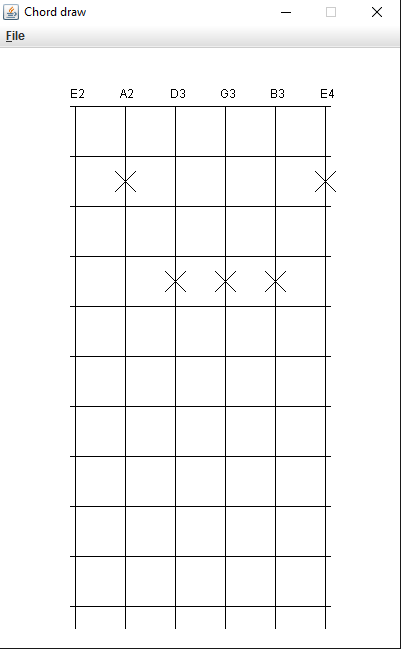
\includegraphics[width=1.0\textwidth]{../img/chords/ChordDraw}
\end{minipage}

\end{Slide}

\begin{Slide}{Modell av gitarr och ukulele}
\begin{Code}
object model {

  type Tuning = Vector[String]
  type Grip = Vector[Int]

  trait Chord {
    def name: String
    def tuning: Tuning
    def grip: Grip
  }
  
  case class Guitar(name: String, grip: Grip) extends Chord {
    val tuning = Vector("E2", "A2", "D3", "G3", "B3", "E4")
  }
  
  case class Ukulele(name: String, grip: Grip) extends Chord {
    val tuning = Vector("G4", "C4", "E4", "A4")
  }

}
\end{Code}
\end{Slide}

\begin{Slide}{En gemensam bastyp för olika ackord}\SlideFontSmall
\vspace{-0.5em}\begin{center}
\newcommand{\TextBox}[1]{\raisebox{0pt}[1em][0.5em]{#1}}
\tikzstyle{umlclass}=[rectangle, draw=black,  thick, anchor=north, text width=3cm, rectangle split, rectangle split parts = 3]
\begin{tikzpicture}[inner sep=0.5em]
\node [umlclass, rectangle split parts = 2, xshift=0cm, text width=5cm] (BaseType)  {
            \textit{\textbf{\centerline{\TextBox{\code{Chord}}}}}
            \nodepart[]{second}
            \TextBox{\code{def name: String}}\vspace{-0.25em}\newline
            \TextBox{\code{def tuning: Vector[String]}}\vspace{-0.25em}\newline
            \TextBox{\code{def grip: Vector[Int]}}\vspace{-0.25em}\newline

        };
        
\node [umlclass, rectangle split parts = 1]  at (2.5cm,-3.7cm) (SubType1) {
            \textbf{\centerline{\TextBox{\code{Guitar}}}}
            %\nodepart[]{second} \TextBox{~}
        };  
                
\node [umlclass, rectangle split parts = 1] at (-2.5cm,-3.7cm) (SubType2)  {
            \textbf{\centerline{\TextBox{\code{Ukulele}}}}
            %\nodepart[]{second} \TextBox{talk(): void}
        };        
\draw[umlarrow] (SubType1.north) -- ++(0,0.5) -| (BaseType.south);    
\draw[umlarrow] (SubType2.north) -- ++(0,0.5) -| (BaseType.south);            
\end{tikzpicture}
\end{center}
\pause\vspace{-0.7em}
\begin{REPL}
scala> import model._

scala> val uc = Ukulele("C", Vector(0, 0, 0, 3))
uc: model.Ukulele = Ukulele(C,Vector(0, 0, 0, 3))

scala> val ge = Guitar("E", Vector(0, 2, 2, 1, 0, 0))
ge: model.Guitar = Guitar(E,Vector(0, 2, 2, 1, 0, 0))
\end{REPL}
\end{Slide}


\begin{Slide}{Grupparbete}\SlideFontSmall
\begin{itemize}
\item Förslag på arbetssätt:
\begin{itemize}\SlideFontSmall
\item Träffas nu på rasten och boka nästa gruppmöte
\item Förberedelser inför första gruppmötet: individuella studier av labbinstruktioner och koden som är given i workspace \\
\href{https://github.com/lunduniversity/introprog/tree/master/workspace/w08_chords_team/src}{.../workspace/w08\_chords\_team/src} \\
OBS! numrering av labbarna enl. ''gamla'' veckor
\item Träffas gärna i ett studierum med whiteboard
\item På mötet: gå igenom uppgift och given kod så att alla fattar vad det går ut på; bestäm omfattning och ansvarsuppdelning
\item När ni träffas, skissa upp den kod som just du håller på med på whiteboard och få feedback och ge feedback till andra
\item På varje gruppmöte, bestäm tid för nästa möte och vad var och en ska försöka hinna tills dess
\end{itemize}


\item Ni får \Emph{lov att ändra på omfattningen} efter antalet gruppmedlemmar, ambition och förmåga: diskutera detta med handledare på resurstid

\item \Alert{Minimikrav}: att med textkommando kunna skapa/spara/ladda gitarr- och ukulele-ackord och att ni tränar på matchning

\end{itemize}
\end{Slide}


\Subsection{Matchning}

\begin{Slide}{Vad är matchning?}
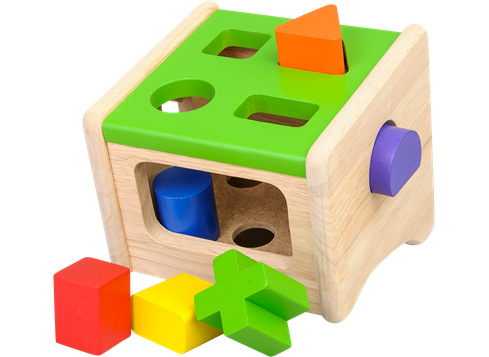
\includegraphics[width=0.8\textwidth]{../img/plocklada.png}
\end{Slide}


\begin{Slide}{Vad är matchning?}
Matchning gör man då man vill jämföra ett värde mot andra värden och hitta överensstämmelse \Eng{match}.

\pause

\vspace{1em}Detta kan man t.ex. göra med nästlade if-else-satser/uttryck:

\begin{Code}
val g = scala.io.StdIn.readLine("grönsak:")
val smak = 
  if (g == "gurka") "gott!"
  else if (g == "tomat") "jättegott!"
  else if (g == "broccoli") "ganska gott..."
  else "inte gott :("

println(g + " är " + smak)
\end{Code}
\end{Slide}




\begin{Slide}{Javas switch-sats}\SlideFontSmall
De flesta C-liknande språk (men inte Scala) har en \jcode{switch}-sats som man kan använda istället för (vissa) nästlade if-else-satser: 
\javainputlisting[basicstyle=\ttfamily\SlideFontSize{5.5}{6.8}\selectfont]{../compendium/examples/match/Switch.java}

\vspace{-0.5em}Funkar bara för primitiva typer och några till (t.ex. String).
\end{Slide}




\begin{Slide}{Javas switch-sats utan break}\SlideFontSmall
Saknad \jcode{break}-sats ''faller igenom'' till efterföljande gren: 

\javainputlisting[basicstyle=\ttfamily\SlideFontSize{6}{7}\selectfont]{../compendium/examples/match/SwitchNoBreak.java}
En glömd \jcode{break} kan ge svårhittad bugg... 
\end{Slide}

\begin{Slide}{Javas switch-sats med glömd break}\SlideFontSmall

\vspace{-0.5em}\javainputlisting[basicstyle=\ttfamily\SlideFontSize{5.5}{6.8}\selectfont]{../compendium/examples/match/SwitchForgotBreak.java}

\vspace{-0.7em}\pause
\begin{REPL}
$ java SwitchForgotBreak 
Skriv grönsak:
gurka
gott!
gott!
\end{REPL}

\end{Slide}


\begin{Slide}{Scalas \texttt{match}-uttryck}\SlideFontSmall
Scala har ingen \code{switch}-sats men erbjuder i stället ett \code{match}-\Emph{uttryck} som är kraftfullare och ger ett värde.

\begin{Code}
val g = scala.io.StdIn.readLine("grönsak:")
val smak = g match {
  case "gurka" => "gott!"
  case "tomat" => "jättegott!"
  case "broccoli" => "ganska gott..."
  case _ => "mindre gott..."
}
println(g + " är " + smak)
\end{Code}
Och den ''faller inte igenom'' som Javas \code{switch}-sats! 
\begin{itemize}
\pause\item Varje \code{case}-gren testas var för sig i tur och ordning uppifrån och ned.
\pause\item Det som står mellan \code{case} och \code{=>} kallas ett \Emph{mönster} \Eng{pattern}
\pause\item Sista default-grenen ovan kallas \Emph{wildcard-mönster}: \code{case _ => } 
\pause\item Ovan är exempel på matchning mot \Emph{konstant-mönster}, \\ i detta fallet tre stycken strängkonstantmönster.
\pause\item Det finns många andra sätt att skriva mönster.
\end{itemize}
\end{Slide}



\begin{Slide}{Matchning med gard}
Man kan stoppa in en s.k \Emph{gard} \Eng{guard} innan pilen \code{=>} för att villkora matchningen: (notera \code{if}, parenteser behövs ej)
\begin{Code}
val g = scala.io.StdIn.readLine("grönsak:")
def f = g match {
  case "gurka" if math.random > 0.5 => "gott ibland!"
  case "tomat" => "jättegott!"
  case "broccoli" => "ganska gott..."
  case _ => "mindre gott..."
}
\end{Code}
\code{case}-grenen med gard ger bara en lyckad matchning \\ om uttrycket efter \code{if} är sant; annars provas nästa gren, etc.
\end{Slide}

\begin{Slide}{Matchning med variabelmönster}\SlideFontSmall
Om det finns ett namn efter \code{case} som börjar med liten begynnelsebokstav, blir detta namn en variabel som automatiskt binds till uttrycket före \code{match}:

\begin{Code}
val g = scala.io.StdIn.readLine("grönsak:")
def f = g match {
  case "gurka" if math.random > 0.5 => "gott ibland!"
  case "tomat" => "jättegott!"
  case "broccoli" => "ganska gott..."
  case other => "smakar bakvänt: " + other.reverse
}
\end{Code}

Ett enkelt variabelmönster, så som \\ \code{case other => ...} \\ i exemplet ovan, matchar \Emph{allt}! \\\code{other} får alltså värdet av \code{g} om \code{g} \Alert{inte} är \code{"gurka"}, \code{"tomat"}, \code{"broccoli"}.  

\end{Slide}





\begin{Slide}{Matchning med typade mönster}\SlideFontSmall
Med en typannotering efter en variabel får man ett \Emph{typat mönster} \Eng{typed pattern}. Om matchningen lyckas blir värdet \Alert{omvandlat} till den specifika typen och binds till variabeln.
\begin{Code}
def f = if (math.random < 0.5) 42 + math.random else "gurka" + math.random
def g = f match {
  case x: Double => x.round.toInt
  case s: String => s.length
}
\end{Code}
Vad har funktionen \code{f} för returtyp? \\ \pause
Matchning mot specifika typer enl. ovan används i idiomatisk Scala hellre än \code{isInstanceOf} men man kan göra motsvarande ovan med if-uttryck:
\begin{Code}
def g2 = {
  val x = f
  if (x.isInstanceOf[Double]) x.asInstanceOf[Double].round.toInt
  else if (x.isInstanceOf[String]) x.asInstanceOf[String].length
}.asInstanceOf[Int]
\end{Code}
\end{Slide}


\begin{Slide}{Konstruktormönster med case-klasser}\SlideFontSmall
En basklass med gemensamma delar och två subtyper:
\begin{Code}
trait Grönsak {
  def vikt: Int
  def ärRutten: Boolean
}
case class Gurka(vikt: Int, ärRutten: Boolean) extends Grönsak
case class Tomat(vikt: Int, ärRutten: Boolean) extends Grönsak
\end{Code}
\pause
Tack vare case-klasserna kan man använda \Emph{konstruktormönster} \Eng{constructor pattern} för att kolla vad som finns \Alert{inuti} en instans:
\begin{Code}
def testa(g: Grönsak): String = g match {
  case Gurka(v, false) => "gott, väger " + v
  case Gurka(_, true)  => "inte gott"
  case Tomat(v, r)     => (if (r) "inte " else "") + "gott, väger " + v 
  case _ => "okänd grönsak: " + g
}
\end{Code}

Konstruktormönster ''\Emph{plockar isär}'' det som matchas och binder variabler till de attribut som finns i case-klassens konstruktor.
\end{Slide}


\begin{Slide}{Plocka isär samlingar med djupa mönster}
Man kan plocka isär innehållet i en samling så här:
\begin{Code}
def visa(xs: Vector[Grönsak]): String = xs match {
  case Vector()               => "tom grönsaksvektor"
  case Vector(Gurka(v, true)) => "en rutten gurka som väger " + v
  case Vector(g)              => "exakt en grönsak: " + g
  case Vector(g1, g2)         => s"exakt två grönsaker: $g1, $g2"
  case g +: gs                => s"först en $g och sedan svansen: $gs" 
}
\end{Code}
Övning: prova ovan i REPL. Vad händer om du byter ordning på andra och tredje mönstret ovan?
\end{Slide}

\begin{Slide}{Mönstermatchning och case-objekt}
En bastyp och specifika singelobjekt av gemensam typ:
\begin{Code}
trait Färg
case object Spader  extends Färg
case object Hjärter extends Färg
case object Ruter   extends Färg
case object Klöver  extends Färg

def parallellFärg(f: Färg): Färg = f match {
  case Spader  => Klöver
  case Klöver  => Spader
  case Hjärter => Ruter
}
\end{Code}
Vilken case-gren har vi glömt? Kan kompilatorn hjälpa oss?
\pause
\begin{REPL}
scala> parallellFärg(Ruter)
scala.MatchError: Ruter (of class Ruter$)
  at .parallellFärg(<console>:18)

\end{REPL}
Runtime exception \code{:(} ~~och en bugg som kan vara svårhittad...
\end{Slide}

\begin{Slide}{Mönstermatchning och förseglade typer}
Med nyckelordet \code{sealed} får vi en kompileringsvarning \code{:)}
\begin{Code}
sealed trait Färg
case object Spader  extends Färg
case object Hjärter extends Färg
case object Ruter   extends Färg
case object Klöver  extends Färg

def parallellFärg(f: Färg): Färg = f match {
  case Spader  => Klöver
  case Klöver  => Spader
  case Hjärter => Ruter
}
\end{Code}
\begin{REPL}
// Exiting paste mode, now interpreting.

<console>:23: warning: match may not be exhaustive.
It would fail on the following input: Ruter
       def parallellFärg(f: Färg): Färg = f match {
\end{REPL}
\end{Slide}

\begin{Slide}{Stora/små begynnelsebokstäver vid matchning}
Fallgrop: att försöka matcha på värdet av en variabel som börjar med liten bokstav.
\begin{REPL}
scala> val livetsMening = 42

scala> def ärLivetsMeningBuggig(svar: Int) = svar match {
         case livetsMening => true    // lokalt namn som matchar allt!
         case _ => false
       }

scala> ärLivetsMeningBuggig(43)
res0: Boolean = true

scala> val LivetsMening = 42   // stor begynnelsebokstav

scala> def ärLivetsMening(svar: Int) = svar match {
         case LivetsMening => true    // funkar fint!
         case _ => false
       }

scala> ärLivetsMening(43)
res1: Boolean = false
\end{REPL}
\end{Slide}


\begin{Slide}{Stora/små begynnelsebokstäver vid matchning}
Ett sätt att komma runt problemet med liten begynnelsebokstav: \\
\Emph{backticks} to the rescue!
\begin{REPL}
scala> val livetsMening = 42

scala> def ärLivetsMeningBackTicks(svar: Int) = svar match {
         case `livetsMening` => true    // nu funkar det!
         case _ => false
       }

scala> ärLivetsMeningBackTicks(43)
res2: Boolean = false
\end{REPL}
\end{Slide}


\begin{Slide}{Mönster på andra ställen än i \texttt{match}}\SlideFontSmall
Mönster i \Emph{deklarationer}:
\vspace{-0.25em}\begin{REPL}
scala> case class Point(x: Int, y: Int)

scala> val p = Point(0, 1)

scala> val Point(x, y) = p          // konstruktormönster med case-klass
x: ???
y: ???

scala> val (x, y, z) = (0, 1, 2)    // konstruktormönster med tupel
x: ???
y: ???
z: ???

\end{REPL}
Mönster i \Emph{for-satser}:
\vspace{-0.25em}\begin{REPL}
scala> val xs = for ((x, y) <- Vector((1,2), (3,4))) yield x
xs: ???
\end{REPL}

\end{Slide}

\begin{Slide}{Mönster på andra ställen än i \texttt{match}}\SlideFontSmall
Mönster i \Emph{deklarationer}:
\vspace{-0.25em}\begin{REPL}
scala> case class Point(x: Int, y: Int)

scala> val p = Point(0, 1)

scala> val Point(x, y) = p          // konstruktormönster med case-klass
x: Int = 0
y: Int = 1

scala> val (x, y, z) = (0, 1, 2)    // konstruktormönster med tupel
x: Int = 0
y: Int = 1
z: Int = 2

\end{REPL}
Mönster i \Emph{for-satser}:
\vspace{-0.25em}\begin{REPL}
scala> val xs = for ((x, y) <- Vector((1,2), (3,4))) yield x
xs: scala.collection.immutable.Vector[Int] = Vector(1, 3)
\end{REPL}
\end{Slide}

\begin{Slide}{Fördjupning om mönster}
Avancerade saker för den intresserade (ingår ej): 
\begin{itemize}
\item binda variabler till mönsterdelar med \code{@}
\item partiella funktioner
\item att skapa extraherare med \code{unapply} och \code{unapplySeq}
\end{itemize}
Fördjupning:
\begin{itemize}
\item Läs mer om mönster här:  \href{http://www.artima.com/pins1ed/case-classes-and-pattern-matching.html}{\SlideFontTiny www.artima.com/pins1ed/case-classes-and-pattern-matching.html}

\item För djupare förståelse av hur \code{case} fungerar, läs speciellt om \Emph{partiella funktioner} här: \href{http://www.artima.com/pins1ed/case-classes-and-pattern-matching.html\#15.7}{\SlideFontTiny www.artima.com/pins1ed/case-classes-and-pattern-matching.html\#15.7}

\item Läs om extractors här: \href{http://www.artima.com/pins1ed/extractors.html}{\SlideFontTiny www.artima.com/pins1ed/extractors.html}

\end{itemize} 
\end{Slide}


\begin{Slide}{Fördjupning: metoden \texttt{unapply}}\SlideFontSmall
När du deklarerar en case-klass kommer kompilatorn att \Alert{automatiskt generera en metod} med namnet \Emph{\texttt{unapply}} som kan plocka isär instansen.
\begin{REPL}
scala> case class Gurka(vikt: Int, ärRutten: Boolean)

scala> Gurka.unapply // tryck TAB två gånger för att se metodhuvudet
 case def unapply(x$0: Gurka): Option[(Int, Boolean)]
 
scala> val g = Gurka(100, false)

scala> Gurka.unapply(g)
res0: Option[(Int, Boolean)] = Some((100,false))
\end{REPL}
Vi ska snart se hur \code{Option} kan hantera värden som \Emph{eventuellt} \Alert{saknas}. \\
\pause

{\SlideFontTiny\vspace{1em}\emph{Fördjupning:} Ett anrop av metoden \code{unapply} genereras av kompilatorn vid matchning och det är det som gör att case-klasser kan användas i konstruktormönster. Man kan skapa en egna s.k. extraktorer \Eng{extractors} som funkar i matchningar (se övn. 22).}
\end{Slide}







%!TEX encoding = UTF-8 Unicode
%!TEX root = ../lect-w10.tex

%%%

\Subsection{Option}


\begin{Slide}{Hur hantera saknade värden?}\SlideFontSmall
Olika sätt att hantera saknade värden:
\begin{itemize}
\item Hitta på ett specialvärde: exempel -1 för icke nedtryckt sträng
\item \code{null} om \code{AnyRef}/\code{Object} (vanligt i Java, mkt ovanligt i Scala) 
\item Använd en samling och låt tom samling representera saknat värde: \\
\code{val grip = Vector(Vector(2), Vector(7), Vector(), Vector(3))}

\item \code{Option[T]} gemensam bastyp för: \\
  \code{None} som representerar \Alert{saknat värde}, och \\ \code{Some[T]} som representerar att \Emph{värde finns}
\end{itemize}
\end{Slide}

\begin{Slide}{En gemensam bastyp för ett värde som kanske saknas}\SlideFontSmall
\vspace{-0.0em}\begin{center}
\newcommand{\TextBox}[1]{\raisebox{0pt}[1em][0.5em]{#1}}
\tikzstyle{umlclass}=[rectangle, draw=black,  thick, anchor=north, text width=3cm, rectangle split, rectangle split parts = 3]
\begin{tikzpicture}[inner sep=0.5em]
\node [umlclass, rectangle split parts = 2, xshift=0cm, text width=3.5cm] (BaseType)  {
            \textit{\textbf{\centerline{\TextBox{\code{Option[A]}}}}}
            \nodepart[]{second}
            \TextBox{\code{def get: A}}\newline
            \TextBox{\code{def isEmpty: Boolean}}

        };
        
\node [umlclass, rectangle split parts = 1]  at (-2.5cm,-3.0cm) (SubType1) {
            \textbf{\centerline{\TextBox{\code{Some[A]}}}}
            % \nodepart[]{second} \TextBox{\code{val x: A}}
        };  
                
\node [umlclass, rectangle split parts = 1] at (2.5cm,-3.0cm) (SubType2)  {
            \textbf{\centerline{\TextBox{\code{None}}}}
        };        
\draw[umlarrow] (SubType1.north) -- ++(0,0.5) -| (BaseType.south);    
\draw[umlarrow] (SubType2.north) -- ++(0,0.5) -| (BaseType.south);            
\end{tikzpicture}
\end{center}
\pause
\vspace{-0.5em}\begin{REPL}
scala> var x: Option[Int] = Some(42)

scala> x.isEmpty
res0: Boolean = false

scala> x = None

scala> x.isEmpty
res1: Boolean = true
\end{REPL}
\end{Slide}


\begin{Slide}{Option för hantering av ev. saknade värden}\SlideFontSmall
Alla vill inte berätta för Facebook vad de har för kön. \\ Förbättra Facebooks kod med ett litet Scala-program:
\begin{Code}
trait Gender
case object Male   extends Gender
case object Female extends Gender

case class Person(name: String, gender: Option[Gender])
\end{Code}
\pause
\begin{REPL}
scala> val p1 = Person("Björn",  Some(Male))
scala> val p2 = Person("Sandra", Some(Female))
scala> val p3 = Person("Andro",  None)
scala> val g2 = p2.gender
scala> def show(g: Option[Gender]): String = g match {
         case Some(x) => x.toString
         case None    => "unknown"
       }
scala> show(g2)
scala> show(p3.gender)
scala> val ps = Vector(p1,p2,p3)
scala> ps.map(_.gender).map(show)
\end{REPL}
\end{Slide}

\begin{Slide}{Några smidiga metoder på \code{Option}}\SlideFontSmall
Metoden \code{getOrElse} gör att man ofta kan undvika matchning.
\begin{Code}
var opt: Option[Int] = None

val x = opt.getOrElse(42)      // get the value or give a default if missing
\end{Code}

Flera av de vanliga samlingsmetoderna funkar, t.ex. \code{foreach} och \code{map}.
\begin{Code}
opt.foreach{x => println(x)}    // only done if value exists

opt.map{x => x + 1}             // only done if value exists

opt = Some(42)                  // change opt to now have some value

opt.foreach{x => println(x)}    // done as value now exists

opt.map{x => x + 1}             // done as value now exists

\end{Code}
\end{Slide}


\begin{Slide}{Några samlingsmetoder som ger en \code{Option}}
\begin{REPL}
scala> val (xs, ys) = (Vector(1,2,3), Vector())

scala> xs.headOption
res0: ???

scala> ys.headOption
res1: ???

scala> xs.find(_ > 1)
res2: ???

scala> xs.find(_ > 5)
res3: ???

scala> val huvudstad = Map("Sverige" -> "Sthlm", "Skåne" -> "Malmö")

scala> huvudstad.get("Skåne")
res4: ???

scala> huvudstad.get("Danmark")
res5: ???
\end{REPL}
\end{Slide}

\begin{Slide}{Några samlingsmetoder som ger en \code{Option}}
\begin{REPL}
scala> val (xs, ys) = (Vector(1,2,3), Vector())

scala> xs.headOption
res0: Option[Int] = Some(1)

scala> ys.headOption
res1: Option[Nothing] = None

scala> xs.find(_ > 1)
res2: Option[Int] = Some(2)

scala> xs.find(_ > 5)
res3: Option[Int] = None

scala> val huvudstad = Map("Sverige" -> "Sthlm", "Skåne" -> "Malmö")

scala> huvudstad.get("Skåne")
res4: Option[String] = Some(Malmö)

scala> huvudstad.get("Danmark")
res5: Option[String] = None
\end{REPL}
\end{Slide}





%!TEX encoding = UTF-8 Unicode
%!TEX root = ../lect-w10.tex

%%%

\Subsection{\texttt{equals}}
\begin{Slide}{Fördjupning: Implementera \texttt{equals} med \texttt{match}}
Det visar sig att \Emph{innehållslikhet} är \Alert{förvånansvärt komplicerat} att implementera, speciellt  i samband med arv.
\begin{itemize}
\item Det enklare fallet: Gör övningsuppgift \code{patterns:14} och implementera \code{equals} för innehållslikhet utan arv. \\ En bra träning på att använda \code{match}!

\item Svårare: Gör fördjupningsövning \code{matching:21--22} om du vill se hur en \emph{komplett} \code{equals} ska se ut som funkar i alla lägen.

\end{itemize}

Det ingår inte på tentan att själv kunna implementera en generellt fungerande \code{equals}. Men du ska förstå skillnaden mellan referenslikhet och innehållslikhet. Mer om \code{equals} i fortsättningkursen, men en liten inblick i problemet nu...
\end{Slide}

\begin{Slide}{Fördjupning: \texttt{equals} som fungerar för finala klasser}
Recept för implementation av \code{equals} som fungerar för typer som \Alert{inte} har några subtyper:
\begin{Code}
final class Gurka(val vikt: Int, ärÄtbar: Boolean) {
  override def equals(other: Any): Boolean = other match {
    case that: Gurka => vikt == that.vikt && ärÄtbar == that.ärÄtbar
    case _ => false
  }
  override def hashCode: Int = (vikt, ärÄtbar).## // ger bra hashcode
}
\end{Code}
\begin{itemize}\SlideFontSmall
  \item
  Du \Alert{måste} alltid överskugga \code{hashCode} också om du överskuggar \code{equals} annars funkar inte gurksamlingar (lång story ...)
  \item
  Notera typen \code{Any} -- detta följer hur man valde att göra i Java (tyvärr?).
  \pause
  \item
  Ett \Alert{typsäkrare} innehållslikhetstest som \Emph{garanterat} bara jämför en gurka med en gurka och inget annat:
  \begin{Code}
    def ===(other: Gurka): Boolean =
      vikt == other.vikt && ärÄtbar == other.ärÄtbar
  \end{Code}
\end{itemize}
\end{Slide}


\begin{Slide}{Fördjupning: Recept i 8 steg för arvssäker \code{equals}}\SlideFontTiny
%fungerar även för klasser som inte är \code{final}:
\setlength{\leftmargini}{0pt}
\begin{enumerate}\SlideFontTiny
\item Inför denna metod: \code{ def canEqual(other: Any): Boolean}\\Observera att typen på parametern ska vara \code{Any}. Om subklass behövs \code{override}.

\item Metoden \code{canEqual} ska ge \code{true} om \code{other} är av samma typ som \code{this}, t.ex.: \code{override def canEqual(other: Any): Boolean = other.isInstanceOf[Gurka]}

\item Inför metoden \code{equals} och var noga med att parametern har typen \code{Any}: \\ \code{override def equals(other: Any): Boolean}

\item Implementera metoden \code{equals} med ett match-uttryck som börjar så här:
\code|other match { ... } |

\item Match-uttrycket ska ha två grenar. Den första grenen ska ha ett typat mönster för den klass som ska jämföras, t.ex.: \\ \code{  case that: Gurka =>}

\item Om du implementerar \code{equals} i den klass som inför \code{canEqual}, börja med: \\ \code{(that canEqual this) &&} \\
och skapa därefter en fortsättning som baseras på innehållet i klassen, t.ex.: \code{this.vikt == that.vikt && this.längd == that.längd} \\
Om du överskuggar equals vill du nog börja med
 \code{super.equals(that) && }

\item Den andra grenen i matchningen ska vara:
\code{case _ => false}

\item Överskugga \code{hashCode}, t.ex. med tupel av attributvärden och metoden \code{##}: \\
\code{override def hashCode: Int  = (vikt, längd).## }

\end{enumerate}
\url{http://www.artima.com/pins1ed/object-equality.html}

\end{Slide}

%!TEX encoding = UTF-8 Unicode
%!TEX root = ../lect-w10.tex

%%%



\Subsection{Undantag}
\begin{Slide}{Vad är ett undantag \Eng{exception}?}
Undantag representerar ett fel eller ett onormalt tillstånd som upptäcks under exekvering och som  behöver hanteras på särskilt sätt vid sidan av det normala exekveringsflödet. 

\vspace{1em}\href{https://sv.wikipedia.org/wiki/Undantagshantering}{sv.wikipedia.org/wiki/Undantagshantering}


\vspace{1em} Exempel på undantag:

\pause

\begin{itemize}
\item Indexering utanför vektorns indexgränser.

\item Läsning bortom filens slut.

\item Försök att öppna en fil som inte finns.

\item Minnet är slut.

\item Division med noll.

\item \code{"hej".toInt} resulterar i \\\code{java.lang.NumberFormatException}

\end{itemize}

\end{Slide}

\begin{Slide}{''Kasta'' dina egna undantag med \texttt{throw}}\SlideFontSmall
Man kan själv generera ett undantag med \code{throw}, vilket kallas att \Emph{kasta} ett undantag som (om det inte \Emph{fångas}), gör att exekveringen \Alert{avbryts}.


\begin{REPL}
scala> def pang = throw new Exception("PANG!")
pang: Nothing

scala> pang
java.lang.Exception: PANG!
  at .pang(<console>:11)
  ...
  
\end{REPL}
\pause
Olika sätt att hantera undantag: 
\begin{itemize}
\item Scala: Man kan använda ett \code{try ... catch}-uttryck och ge ett \Emph{värde} i händelse av undantag.
\item Java: Man kan använda en \code{try ... catch}-sats och \Alert{göra något} i händelse av undantag.
 
\item Scala: Man kan \Emph{kapsla in} ett undantag med \Emph{\texttt{scala.util.Try}} och förhindra att exekveringen avbryts. (Finns ej i Java; att föredra i Scala.)
\end{itemize}
\end{Slide}


\Subsection{\texttt{scala.util.Try}}

\begin{Slide}{En gemensam bastyp för något som kan misslyckas}\SlideFontSmall
\begin{Code}
import scala.util.{Try, Success, Failure}
\end{Code}

\vspace{-0.5em}\begin{center}
\newcommand{\TextBox}[1]{\raisebox{0pt}[1em][0.5em]{#1}}
\tikzstyle{umlclass}=[rectangle, draw=black,  thick, anchor=north, text width=3.0cm, rectangle split, rectangle split parts = 3]
\begin{tikzpicture}[inner sep=0.5em]
\node [umlclass, rectangle split parts = 2, xshift=0cm, text width=3.8cm] (BaseType)  {
            \textit{\textbf{\centerline{\TextBox{\code{Try[T]}}}}}
            \nodepart[]{second}
            \TextBox{\code{def get: T}}\newline
            \TextBox{\code{def isFailure: Boolean}}\newline
            \TextBox{\code{def isSuccess: Boolean}}
        };
        
\node [umlclass, rectangle split parts = 2, text width=2.2cm]  at (-2.5cm,-3.7cm) (SubType1) {
            \textbf{\centerline{\TextBox{\code{Success[T]}}}}
            \nodepart[]{second} \TextBox{\code{val value: T}}
        };  
                
\node [umlclass, rectangle split parts = 2, text width=4.2cm] at (2.5cm,-3.7cm) (SubType2)  {
            \textbf{\centerline{\TextBox{\code{Failure[T]}}}}
            \nodepart[]{second} \TextBox{\code{val exception: Throwable}}
        };        
\draw[umlarrow] (SubType1.north) -- ++(0,0.5) -| (BaseType.south);    
\draw[umlarrow] (SubType2.north) -- ++(0,0.5) -| (BaseType.south);            
\end{tikzpicture}
\end{center}
\end{Slide}

\begin{Slide}{Hantera undantag med \texttt{Try}}
\vspace{-0.5em}\begin{REPL}
scala> def pang = throw new Exception("PANG!")

scala> def kanskePang = if (math.random < 0.5) 42 else pang

scala> import scala.util.{Try, Success, Failure}

scala> def försök = Try { kanskePang }

scala> val xs = Vector.fill(15){försök}

scala> val trettonde = xs(13) match {
         case Success(value) => value
         case Failure(e) => println(e); -1
       }

scala> (xs(13).isSuccess, xs(13).isFailure)

scala> försök.foreach(println)

scala> försök.map(_ + 1)

scala> for (Success(x) <- xs) yield x
\end{REPL}
\end{Slide}

\begin{Slide}{Fördjupning: \texttt{try}-\texttt{catch}-uttryck}\SlideFontSmall
Man kan fånga undantag med ett \code{try ... catch}-uttryck:
\begin{Code}
def carola = try {
  if (math.random > 0.5) throw new Exception("stormvind")
  42
} catch { 
  case e: Exception =>
    println("Fångad av en " + e.getMessage)
    -1
}  
\end{Code}
\pause
\begin{REPL}
scala> Vector.fill(5)(carola)
Fångad av en stormvind
Fångad av en stormvind
Fångad av en stormvind
res0: scala.collection.immutable.Vector[Int] = Vector(-1, 42, 42, -1, -1)
\end{REPL}
\pause
\emph{Fördjupning:} \\ Gör övning 9-10 som visar hur man fångar undantag i Scala och Java. \\Mer om undantag i fortsättningskursen.
\end{Slide}








\Lecture{11}{Scala \& Java}
%!TEX encoding = UTF-8 Unicode
%!TEX root = ../lect-w11.tex

%%%


\Subsection{Veckans lab: \texttt{javatext}}
\begin{Slide}{Veckans lab: \texttt{javatext}}\SlideFontSmall
\Emph{Förberedelse:}
\begin{itemize}
\item Gör övning \texttt{scalajava}:
\begin{itemize}\SlideFontSmall
\item Översätt spelet Hangman från Java till Scala
\item Översätt Point från Scala till Java
\item Undersök autoboxning \Eng{autoboxing}
\item Använda \code{import scala.collection.JavaConverters._}
\end{itemize}
\item Studera riktlinjerna för \code{javatext} i kompendiet.
\item Labben är indivuell men du ska spela någon annans spel och ge feedback på koden och någon annan ska spela ditt spel och ge feedback på koden.
\end{itemize}
\Emph{Laboration \code{javatext}}
\begin{itemize}
\item Gör ett (lagom) intressant/roligt textspel för terminalen med ca 80\% Java-kodrader och ca 20\% Scala-kodrader, enligt kraven som beskrivs i kompendiet. Du ska även spela någon annans spel och ge återkoppling.
\end{itemize}
\end{Slide}

%!TEX encoding = UTF-8 Unicode
%!TEX root = ../lect-w11.tex

%%%


\Subsection{Jämförelse Scala och Java}
\begin{Slide}{Grundläggande likheter och skillnader}\SlideFontSmall
\Emph{Några likheter:}
\begin{itemize}\SlideFontTiny
\item Kompilerar till bytekod som kör på JVM på många olika plattformar
\item Statisk typning: snabb maskinkod och kompilatorn hittar buggar vid kompilering
\end{itemize}

\Emph{Liknande men} \Alert{viss skillnad:}\vspace{-1em}
\begin{multicols}{2}
\Emph{Java}
\begin{itemize}\SlideFontTiny
\item \Emph{Objektorientering}, men inte ''äkta'' \Eng{pure} eftersom inte alla värden är objekt

\item Primitiva typer är inte objekt; representeras effektivt, normalt \Emph{utan boxning}

\item Visst stöd för \Emph{funktionsprogrammering}

\item Typer måste alltid anges, ibland två gånger (variabeldeklaration + instansiering)
\end{itemize}

\columnbreak

\Emph{Scala}
\begin{itemize}\SlideFontTiny
\item \Emph{Äkta objektorienterat} eftersom alla värden är objekt, även funktioner

\item \code{AnyVal}-instanser är äkta objekt men representeras ändå effektivt, normalt \Emph{utan boxning} 

\item Omfattande stöd för \Emph{funktionsprogrammering}

\item Typinfo ska finnas vid kompileringstid men kan ofta härledas av kompilatorn
\end{itemize}

\end{multicols}
\end{Slide}




\begin{Slide}{Några saker som finns i Scala men inte i Java}\SlideFontSmall
\vspace{-1em}\begin{multicols}{2}
\begin{itemize}\SlideFontSize{7}{8}
\item \code{case}-klasser

\item Lokala funktioner

\item Metoder som operatorer 

\item Infix operatornotation

\item Defaultargument

\item Namngivna argument

\item Engångsinitialisering: \code{val}

\item Fördröjd initialisering: \code{lazy val}

\item Enhetlig access för \code{def}, \code{val}, \code{var}

\item Egna setters med \code{def namn_=}

\item Namnanrop, fördröjd evaluering

\item Matchning, mönster och garder

\item Klassparametrar, primärkonstruktor

\item Singelobjekt: \code{object}

\item Kompanjonsobjekt

\item Inmixning: \code{trait} 

\item \code{for}-\code{yield}-uttryck

\item Block är uttryck; slipper \code{return}

\item Tomma värdet () av typen \code{Unit}

\item Option, Some, None

\item Try, Success, Failure

\item Samlingarna i Scalas standardbibliotek, speciellt de \Emph{oföränderliga} samlingarna \code{Vector}, \code{Map}, \code{Set}, \code{List}, etc.

\item Enhetlig användning av samlingar inkl. Array

\item Innehållslikhet med \code{==} för oföränderliga strukturer, inkl. \code{< <= > >= } på strängar

\item Implicita värden och klasser

\item Mer precis synlighetsreglering, \code{private[this]}, \code{private[mypackage]}

\item Flexibilitet och namnändring vid \code{import} 

\item Flexibel filstruktur och filnamngivning

\item Flexibel nästling av klasser, objekt, traits

\item Typ-alias och abstrakta typer med \code{type}

\item Implicita värden och klasser

\item ...
\end{itemize}
\end{multicols}
\end{Slide}


\begin{Slide}{Några saker som finns i Java men inte i Scala}\SlideFontSmall
\vspace{-0.7em}\begin{multicols}{2}
\begin{itemize}\SlideFontSize{7.5}{8.5}
\item Variabeldeklaration utan initialisering

\item Förändringsbara parametrar

\item C-liknande prefix- och postfix-inkrementering och -dekrementering: \code{i++ ++i i-- --i}

\item C-liknande \code{for}-sats

\item Semikolon efter alla satser

\item Parenteser efter alla metoder

\item Specialsyntax för indexering av array \code{[]} ej som i andra samlingar

\item Uppräknade typer med {\texttt{\bfseries{\color{eclipsepurple}{enum}}}}

\item Hoppa ut ur loop med \jcode{break} \\ \href{https://docs.oracle.com/javase/tutorial/java/nutsandbolts/branch.html}{\SlideFontSize{5.2}{8.5}docs.oracle.com/javase/tutorial/java/nutsandbolts/branch.html}

\item \jcode{switch} ''faller igenom'' utan \jcode{break}

\item Nästan alltid snabbare kompilering

\item Mer omfattande IDE-stöd

\item Kontrollerade undantag \Eng{checked exceptions} och \jcode{throws}

\item ...
\end{itemize}

\end{multicols}
\end{Slide}





\begin{Slide}{Huvudprogram i Scala och Java}
\begin{multicols}{2}
\Emph{Scala}
\begin{CodeSmall}[basicstyle=\ttfamily\SlideFontSize{6}{8}]
object Main {
  def main(args: Array[String]): Unit = {
    println("Hello!")
  }
}
\end{CodeSmall}

\columnbreak

\Emph{Java}
\begin{CodeSmall}[language=Java,basicstyle=\ttfamily\SlideFontSize{6}{8}]
public class JMain {
  public static void main(String[] args){
    System.out.println("Hello!");
  }
}
\end{CodeSmall}
\end{multicols}
\end{Slide}



\begin{Slide}{Syntax för variabeldeklaration i Scala och Java}\SlideFontSmall
Exempel på variabeldeklarationer i
\begin{multicols}{2}
\Emph{Scala}
\begin{CodeSmall}[basicstyle=\ttfamily\SlideFontSize{8}{10}]
  var i1: Int = 0
  var i2 = 0
  var i3 = 0: Int
  var p = new Point(0, 0)
  var (x, y) = (0, 0)        
  val a = 0
  final val Constant = 42
\end{CodeSmall}
\begin{itemize}\SlideFontTiny
\item i2 härledd typ; går ej i Java

\item i3 typ i uttryck; går ej i Java

\item (x, y) mönster i init; går ej i Java

\item \code{val} ger ''engångsinit''; ingen exakt motsvarighet i Java men \code{final} kan ofta användas i stället
\end{itemize}

\columnbreak

\Emph{Java}
\begin{CodeSmall}[language=Java,basicstyle=\ttfamily\SlideFontSize{8}{10}]
  int i1 = 0;
  int i4;
  Point p = new Point(0, 0);
  final int CONSTANT = 42;
\end{CodeSmall}
\begin{itemize}\SlideFontTiny
\item i4 ej explicit init; går ej i Scala
\end{itemize}
\end{multicols}

\end{Slide}




\begin{Slide}{For-sats i Scala och Java}
\begin{multicols}{2}
\Emph{Scala}
\begin{CodeSmall}[basicstyle=\ttfamily\SlideFontSize{6}{8}]
val s = "Abbasillen"

// Loopa över index framlänges:
  
for (i <- s.indices) {
  println(s(i))
}
  
// Loopa över index baklänges:
 
for (i <- s.indices.reverse) {
  println(s(i))
}
\end{CodeSmall}

\columnbreak

\Emph{Java}
\begin{CodeSmall}[language=Java,basicstyle=\ttfamily\SlideFontSize{6}{8}]
String s = "Abbasillen";

// Loopa över index framlänges:

for (int i = 0; i < s.length(); i++) {
    System.out.println(s.charAt(i));
}

// Loopa över index baklänges:
 
for (int i = s.length()-1; i >= 0; i--) {
    System.out.println(s.charAt(i));
}
\end{CodeSmall}
\end{multicols}
\end{Slide}



\begin{Slide}{For-sats i Scala och Java}
\begin{multicols}{2}
\Emph{Scala}
\begin{CodeSmall}[basicstyle=\ttfamily\SlideFontSize{6}{8}]
val s = "Abbasillen"

// Loopa över index framlänges:
  
for (i <- 0 until s.length) { 
  println(s(i))
}
  
// Loopa över index baklänges:
 
for (i <- s.length-1 to 0 by -1) { 
  println(s(i))
}  
\end{CodeSmall}

\columnbreak

\Emph{Java}
\begin{CodeSmall}[language=Java,basicstyle=\ttfamily\SlideFontSize{6}{8}]
String s = "Abbasillen";

// Loopa över index framlänges:

for (int i = 0; i < s.length(); i++) {
    System.out.println(s.charAt(i));
}

// Loopa över index baklänges:
 
for (int i = s.length()-1; i >= 0; i--) {
    System.out.println(s.charAt(i));
}
\end{CodeSmall}
\end{multicols}
I Scala är \code{s.indices} att föredra!
\end{Slide}



\begin{Slide}{For-each-sats i Scala och Java}
\begin{multicols}{2}
\Emph{Scala}
\begin{CodeSmall}[basicstyle=\ttfamily\SlideFontSize{6}{8}]
val s = "Abbasillen"

// Loopa över alla tecken:

for (ch <- s) {
  println(ch)
}
\end{CodeSmall}

\columnbreak

\Emph{Java}
\begin{CodeSmall}[language=Java,basicstyle=\ttfamily\SlideFontSize{6}{8}]
String s = "Abbasillen";

// Loopa över alla tecken:

for (char ch: s.toCharArray()) {
  System.out.println(ch);
}
\end{CodeSmall}
\end{multicols}

\pause\code{s.foreach(println)       } går ej i Java
\end{Slide}





\begin{Slide}{Exempel: oföränderlig klass i Scala och Java}\SlideFontTiny
\vspace{-1em}
\begin{multicols}{2}
%\Emph{Scala:}
\begin{CodeSmall}[basicstyle=\ttfamily\SlideFontSize{5.7}{6.7}]
class Person(val name: String, val age: Int){
  def isAdult = age >= Person.AdultAge
}

object Person {
  val AdultAge = 18
}
\end{CodeSmall}

\columnbreak

\pause
%\Emph{Java:}
\begin{CodeSmall}[language=Java,basicstyle=\ttfamily\SlideFontSize{5.7}{6.7}]
public class JPerson {
    private String name;
    private int age;
    static final int ADULT_AGE = 18;
      
    public JPerson(String name, int age) {
      this.name = name;
      this.age = age;
    }

    public String getName() {
        return name;
    }

    public int getAge() {
        return age;
    }
    
    public boolean isAdult() {
        return age >= ADULT_AGE;
    }
}
\end{CodeSmall}
Lär dig detta mönster utantill så du snabbt får grejerna på plats!
\end{multicols}
\pause\vspace{-11em} 
\Alert{Övning:}\\Gör \code{Person} + \code{JPerson} \Alert{förändringsbara}\\så att namnet och åldern går att uppdatera\\och följande krav uppfylls:
\begin{itemize}
\item namnet ska ges vid konstruktion,
\item åldern ska initieras till 0 vid konstr.,
\item åldern ska aldrig kunna bli negativ.
\end{itemize}
\end{Slide}


\begin{Slide}{Exempel: förändringsbar klass i Scala och Java}\SlideFontTiny
\vspace{-1.75em}
\begin{multicols}{2}

\begin{CodeSmall}[basicstyle=\ttfamily\SlideFontSize{5}{6}]
class MutablePerson(var name: String) {
  private var _age = 0
 
  def age: Int = _age
  
  def age_=(a: Int): Unit = 
    if (a >= 0) _age = a else _age = 0  //undantag?
  
  def isAdult: Boolean = age >= Person.AdultAge
}

object MutablePerson {
  val AdultAge = 18
}
\end{CodeSmall}

\columnbreak

\pause

\begin{CodeSmall}[language=Java,basicstyle=\ttfamily\SlideFontSize{5}{6}]
public class JMutablePerson {
    private String name;
    private int age = 0;
    static final int ADULT_AGE = 18;
      
    public JMutablePerson(String name) {
      this.name = name;
    }

    public String getName() {
        return name;
    }

    public void setName(String name) {
        this.name = name;
    }

    public int getAge() {
        return age;
    }
    
    public void setAge(int age) {
        if (age >= 0) {
          this.age = age;
        } else {
          this.age = 0;
        }
    }
    
    public boolean isAdult() {
        return age >= ADULT_AGE;
    }
}
\end{CodeSmall}
\end{multicols}

\end{Slide}


\begin{Slide}{Övning: Implementera dessa specifikationer}
\begin{multicols}{2}

{\hskip-0.31em\colorbox{black!70}{\parbox{\dimexpr0.44\textwidth-20\fboxsep-1.9\fboxrule\relax}{\fontsize{7}{8}\selectfont\color{white}{\textit{Specification} \textbf{Vegetable}}}}}

\vspace{-2em}
\begin{CodeSmall}
/** Representerar en grönsak. */
class Vegetable(val name: String) {

  /** Returnerar nuvarande vikt i gram. */
  def weight: Int = ???
  
  /** Ändrar vikten till w gram.
   *  w ska vara positiv, blir annars 0 */
  def weight_=(w: Int): Unit = ???
}
\end{CodeSmall}

\columnbreak

\begin{JavaSpec}{class JVegetable}
/** Skapar en grönsak. */
JVegetable(String name);

/** Returnerar namnet. */
String getName();

/** Returnerar nuvarande vikt i gram. */
int getWeight();

/** Ändrar vikten till weight gram.
 *  w ska vara positiv, blir annars 0 */    
void setWeight(int weight);
\end{JavaSpec}
\end{multicols}
\pause\SlideFontTiny
Fördjupning:\\ Kasta undantaget \code{IllegalArgumentException} vid försök till negativ vikt.\\
Läs om undantag i Java här: \href{https://docs.oracle.com/javase/tutorial/essential/exceptions/index.html}{docs.oracle.com/javase/tutorial/essential/exceptions/}

\end{Slide}




\begin{Slide}{Oföränderlig datatyp i Scala och Java}\SlideFontTiny
\vspace{-0.5em}
\begin{multicols}{2}

En oföränderlig datatyp implementeras i \Emph{Scala} helst som en \pause\code{case}-klass:

\begin{CodeSmall}[basicstyle=\ttfamily\SlideFontSize{5.7}{6.7}]
case class Person(name: String, age: Int) {
  def isAdult = age >= Person.AdultAge
}

object Person {
  val AdultAge = 18
}
\end{CodeSmall}

\columnbreak

En oföränderlig datatyp i \Emph{Java} med \Alert{motsvarande} funktionalitet kräver egen implementation av dessa metoder: 
\vspace{-0.25em}
\begin{itemize}
\item en getter för varje attribut
\item \code{equals}
\item \code{hashcode} (förklaras i forts.kurs)
\item \code{apply} \\ (men man kallar nog den \code{create} el. likn.; namnet måste ju skrivas)
\item \code{toString}
\item \code{copy} \\ (men det finns ju inte namngivna parametrar och defaultargument så denna blir osmidig)
\item \code{unapply} \\ (men det finns ju inte mönstermatchning så denna struntar man nog i)
\end{itemize}

\end{multicols}

\end{Slide}




\Subsection{Array}

\begin{Slide}{Repetition: Primitiva Array i JVM}
\begin{itemize}
\item Primitiva arrayer (\code{Array} i Scala, \code{[]} i Java) har \Emph{fördelar}:%
\footnote{\href{http://stackoverflow.com/questions/2843928/benefits-of-arrays}{stackoverflow.com/questions/2843928/benefits-of-arrays}} 
\begin{itemize}\footnotesize
\item Det är den snabbaste indexerbara datastrukturen i JVM: att läsa och uppdatera ett element på en viss plats är mycket effektivt om man vet platsens index. 
\item Fungerar lika bra med både primitiva värden och objektreferenser
\end{itemize}
\item ... men också \Alert{nackdelar}:
\begin{itemize}\footnotesize
\item Man måste bestämma sig för antalet element som ska allokeras när man gör \code{new}. 
\item Man kan ta i lite extra när man allokerar om man behöver plats för fler senare, men då måste man hålla reda på hur många platser man använder och veta var nästa lediga plats finns.
\item Det är krångligt att stoppa in \Eng{insert} och ta bort \Eng{delete} element.
\item Vill man ha fler platser måste man allokera en helt ny, större array och kopiera över alla befintliga element.
\end{itemize}

\end{itemize}
\end{Slide}




\begin{Slide}{Syntax för Array i Scala och Java}
\begin{multicols}{2}
\Emph{Scala}

\begin{CodeSmall}[basicstyle=\ttfamily\SlideFontSize{6}{8}]
var xs = Array(42, 43, 44)




val n = xs.length

var strings = new Array[String](42)

strings(0) = "first"

strings(1) = "second"
\end{CodeSmall}

\columnbreak

\Emph{Java}

\begin{CodeSmall}[language=Java,basicstyle=\ttfamily\SlideFontSize{6}{8}]
int[] xs = new int[]{42, 43, 44};

// samma som ovan, men kortare:
int[] xs2 = {42, 43, 44}; 

int n = xs.length;  // OBS! EJ length()

String[] strings = new String[42];

strings[0] = "first";

strings[1] = "second";
\end{CodeSmall}

\end{multicols}
\end{Slide}






\begin{Slide}{Exempel: Polygon med primitiv array i Java}
\begin{Code}[numberstyle=,numbers=left,language=Java]
public class Polygon {
    private Point[] vertices; // array med hörnpunkter
    private int n;            // antalet hörnpunkter
    
    /** Skapar en polygon */
    public Polygon() {
        vertices = new Point[1];
        n = 0;
    }
    
    ...
\end{Code}
\end{Slide}

\begin{Slide}{Polygon med primitiv array i Java: \\stoppa in sist och vid behov skapa mer plats}\SlideFontSmall
Implementera:\\
\jcode{private void extend()                // dubbla storleken}\\
\jcode{public void addVertex(int x, int y)  // lägg till hörnpunkt}
\pause
\begin{Code}[numberstyle=,numbers=left,language=Java]
    private void extend(){
        Point[] oldVertices = vertices;
        vertices = new Point[2 * vertices.length]; // skapa dubbel plats
        for (int i = 0; i < oldVertices.length; i++) {  // kopiera
            vertices[i] = oldVertices[i];
        }        
    }

    public void addVertex(int x, int y) {
        if (n == vertices.length) extend();
        vertices[n] = new Point(x, y);
        n++;
    }
\end{Code}
\end{Slide}


\begin{Slide}{Polygon med primitiv array i Java: \\stoppa in mitt i på angiven plats }\SlideFontSmall
Implementera:\\
\jcode{/** Sätt in hörnpunkt på plats pos */}\\
\jcode{public void insertVertex(int pos, int x, int y)}
\pause
\begin{Code}[numberstyle=,numbers=left,language=Java]
    public void insertVertex(int pos, int x, int y) {
        if (n == vertices.length) extend();   // utöka vid behov
        for (int i = n; i > pos; i--) {       // flytta element bakifrån
            vertices[i] = vertices[i - 1];
        }
        vertices[pos] = new Point(x, y);
        n++;
    }
\end{Code}
\end{Slide}





\Subsection{ArrayList}

\begin{Slide}{Generiska samlingar i Java}
\begin{itemize}
\item Från och med version 5 av Java (2004) så introducerades \Emph{generics} vilket möjliggör skapandet av klasser som kan erbjuda generell behandling av olika typer av objekt. 

\item Generiska klasser i Java känns igen med syntaxen \code{Klassnamn<Typ>}, till exempel  \code{ArrayList<Point>}  

\item Fördjupning: \href{https://docs.oracle.com/javase/tutorial/extra/generics/intro.html}{docs.oracle.com/javase/tutorial/extra/generics/intro.html}, mer om detta i fördjupningskursen.

\end{itemize}
\end{Slide}

\begin{Slide}{Om ArrayList i Java}\SlideFontSmall
\code{java.util.ArrayList} liknar \code{scala.collection.mutable.ArrayBuffer} som båda har dessa fördelar:
\begin{itemize}
\item Lagrar sina element internt i snabbindexerade primitiva arrayer.
\item Fungerar för alla typer av objekt.
\item Utökar samlingens storlek av sig själv vid behov.
\end{itemize}
Det finns dock vissa nackdelar med \code{ArrayList} i Java\\(som inte gäller för \code{ArrayBuffer} i Scala):
\begin{itemize}
\item Fungerar \Alert{inte} rakt av med primitiva typer \code{int}, \code{double}, \code{char}, ... \\ (men det finns sätt komma runt detta, tack vare s.k. wrapper-klasser och autoboxing; mer om detta snart)

\item Namnet \code{ArrayList} är inte helt lyckat, eftersom ordet ''lista'' normalt används för länkade snarare än array-liknande strukturer.
\end{itemize}
\end{Slide}

\begin{Slide}{Polygon med ArrayList i Java}\SlideFontSmall
Klassen \code{Polygon}, nu med ett attribut av typen \code{ArrayList<Point>}:
\begin{Code}[numberstyle=,language=Java]
public class Polygon {
    private ArrayList<Point> vertices; // lista med hörnpunkter
    
    /** Skapar en polygon */
    public Polygon() {
        vertices = new ArrayList<Point>();
    }
    
    ...
\end{Code}
Det behövs inget attribut \code{n} eftersom vi inte själva behöver hålla reda på antalet allokerade platser: allokering, insättning, och utökning av antalet platser sköts helt automatiskt av \code{ArrayList}-klassen vid behov. 
\end{Slide}

\begin{Slide}{Viktiga operationer på ArrayList (Urval)}
\begin{JavaSpec}{class ArrayList}
/** Skapar en ny lista */
ArrayList<E>();

/** Tar reda på elementet på plats pos */
E get(int pos);

/** Lägger in objektet obj sist */
void add(E obj);

/** Lägger in obj på plats pos; efterföljande flyttas */
void add(int pos, E obj);

/** Tar bort elementet på plats pos och returnerar det */
E remove(int pos);

/** Tar reda på antalet element i listan */
int size();
\end{JavaSpec}
Lär dig vad som finns om ArrayList i snabbreferensen för Java\\
\SlideFontSmall Överkurs för den nyfikne: kolla implementation av ArrayList \href{http://www.docjar.com/html/api/java/util/ArrayList.java.html}{här}.
\end{Slide}


\begin{Slide}{Övning ArrayList: new och add}
Skriv Java-kod som skapar en lista med element av typen \code{Point} och lägger in tre punkter i listan med koordinaterna:\\ (50, 50), (50,10) och (30, 40).
\pause
\\\vspace{1em} Lösning: \\\vspace{1em} 
\begin{Code}[numberstyle=,language=Java]
ArrayList<Point> vertices = new ArrayList<Point>(); 
vertices.add(new Point(50, 50));
vertices.add(new Point(50, 10)); 
vertices.add(new Point(30, 40)); 
\end{Code}
\end{Slide}


\begin{Slide}{For-each-sats i Java:}\SlideFontSmall
\begin{itemize}
\item  Antag att vi vill gå igenom alla element i en lista. 
\begin{Code}[numberstyle=,language=Java]
        ArrayList<String> words = new ArrayList<String>();
\end{Code}
\item Det finns två olika typer av \jcode{for}-satser i Java som kan göra detta:
\begin{itemize}\footnotesize
\item[]  Vanlig \jcode{for}-sats:
\begin{Code}[numberstyle=,language=Java]
for (int i = 0; i < words.size(); i++) {
    System.out.println(i + ": " + words.get(i));
}
\end{Code}

\item[]  Så kallad \Emph{for-each-sats} med denna syntax:\\
\jcode+for (Elementtyp element: samling) { ... }+ \\
\vspace{1em}Exempel:
\begin{Code}[numberstyle=,language=Java]
for (String s: words) {
    System.out.println(s);
}
\end{Code}
Men vi får ingen indexvariabel då...
\end{itemize}
\end{itemize}
\end{Slide}


\begin{Slide}{Polygon med ArrayList: metoderna blir enklare}
\begin{Code}[numberstyle=,language=Java]
    public void addVertex(int x, int y) {  
        vertices.add(new Point(x, y));
    }
    
    public void move(int dx, int dy) {
        for (Point p: vertices){
            p.move(dx, dy);
        }
    }
    
    public void insertVertex(int pos, int x, int y) {
        vertices.add(pos, new Point(x, y));
    }
    
    public void removeVertex(int pos) {
        vertices.remove(pos);
    }
\end{Code}

Se hela lösningen här:
\href{https://github.com/lunduniversity/introprog/tree/master/compendium/examples/scalajava/list/Polygon.java}{compendium/examples/scalajava/list/Polygon.java}
\end{Slide}

\begin{Slide}{Polygon med ArrayList: \\iterera över alla hörnpunkter i draw med indexering}
\begin{Code}[numberstyle=,language=Java]
    public void draw(SimpleWindow w) {
        if (vertices.size() == 0) {
            return;
        }
        Point start = vertices.get(0);
        w.moveTo(start.getX(), start.getY());
        for (int i = 1; i < vertices.size(); i++) {
            w.lineTo(vertices.get(i).getX(), 
                     vertices.get(i).getY());
        }
        w.lineTo(start.getX(), start.getY());
    }
\end{Code}

Övning: Skriv om med for-each-sats.
\end{Slide}

\begin{Slide}{Polygon med ArrayList: \\iterera över alla hörnpunkter i draw med foreach-sats}
\begin{Code}[numberstyle=,language=Java]
    public void draw(SimpleWindow w) {
        if (vertices.size() == 0) {
            return;
        }
        Point start = vertices.get(0);
        w.moveTo(start.getX(), start.getY());
        for (Point p: vertices){
            w.lineTo(p.getX(), p.getY());
        }
        w.lineTo(start.getX(), start.getY());
    }
\end{Code}

Se hela lösningen här:
\href{https://github.com/lunduniversity/introprog/tree/master/compendium/examples/scalajava/list/Polygon.java}{compendium/examples/scalajava/list/Polygon.java}
\end{Slide}




\begin{Slide}{Övning ArrayList: implementera metoden hasVertex}
Skriv kod som implementerar denna metod i klassen \code{Polygon}:
\begin{Code}[numberstyle=,language=Java]
/** Undersöker om polygonen har någon hörnpunkt med koordinaterna x, y. */ 
public boolean hasVertex(int x, int y) {
    ???
} 
\end{Code}
\end{Slide}

\begin{Slide}{Övning ArrayList: implementera metoden hasVertex}
\begin{Code}[numberstyle=,language=Java]
    public boolean hasVertex(int x, int y) {
        for (Point p: vertices) {
            if (p.getX() == x && p.getY() == y) {
                return true;
            }
        }
        return false;
    }
\end{Code}
\end{Slide}


\begin{Slide}{For-each-sats med array}
For-each-sats fungerar även med primitiv array:
\begin{Code}[numberstyle=,language=Java]
        String[] stringArray = {"hej", "på", "dej"};
        for (String s: stringArray) {
            System.out.println(s);
        }
\end{Code}
\end{Slide}





\Subsection{Autoboxing}



\begin{Slide}{Generiska klasser (t.ex. ArrayList) med primitiva typer}
\begin{itemize}\footnotesize
\item Men vad gör man om man vill ha element av primitiva typer, \\ så som \jcode{int} och \jcode{double}? 
Detta går alltså \Alert{INTE} i Java: \\
\sout{\texttt{ArrayList<int> list = new ArrayList<int>();}}

\vspace{2em}
\item Javas lösning på problemet består av två delar:
\begin{itemize}\footnotesize
\item Klasser som packar in primitiva typer, \Eng{wrapper classes}
\item Speciella regler för implicita konverteringar, s.k. ''auto-boxing'' \Eng{Boxing / Unboxing conversions}
\end{itemize}
\end{itemize}
\scriptsize\vspace{1em}
Detta kan bli ganska komplicerat och det finns fallgropar.\\
(Om du är nyfiken på alla intrikata detaljer, se
\href{https://docs.oracle.com/javase/tutorial/java/data/autoboxing.html}{Java tutorial} och   \href{https://docs.oracle.com/javase/specs/jls/se8/html/jls-5.html#jls-5.1.7}{Javaspecifikationen}.)
\end{Slide}

\begin{Slide}{Wrapper-klassen \code{Integer}}\footnotesize
En skiss av klassen \code{Integer} \\ (ligger i paketet \href{http://docs.oracle.com/javase/8/docs/api/java/lang/package-summary.html}{\code{java.lang}} och importeras därmed implicit):

\begin{minipage}{0.65\textwidth}
\begin{Code}[numberstyle=,language=Java]
public class Integer {
    private int value;
    
    public static final MIN_VALUE = -2147483648;
    public static final MAX_VALUE = 2147483647;
    
    public Integer(int value) {
        this.value = value;
    }
    
    public int intValue() {
        return value;
    }
    ...
}
\end{Code}
\end{minipage}
\begin{minipage}{0.33\textwidth}
\centering
\includegraphics[width=0.95\textwidth]{../img/box}
\end{minipage}
Javadoc för klasen \code{Integer} finns här: \\
\scriptsize\url{http://docs.oracle.com/javase/8/docs/api/java/lang/Integer.html}
\end{Slide}





\begin{Slide}{Wrapper-klasser i \code{java.lang}}\footnotesize
\begin{tabular}{l | l}
\Emph{Primitiv typ}                  & \Emph{Inpackad typ}                 \\ \hline

 boolean & Boolean\\
 byte & Byte\\
 short& Short\\
 char & Character\\
 int & Integer\\
 long & Long\\
 float & Float\\
 double & Double\\
\end{tabular}
\end{Slide}


\begin{Slide}{Övning: primitiva versus inpackade typer}
Med papper och penna:
\begin{itemize}
\item Deklarera en variabel med namnet  \code{gurka} av den primitiva heltalstypen och initiera den till värdet 42.
\item Deklarera en referensvariabel med namnet  \code{tomat} av den inpackade (''wrappade'') heltalstypen och initiera den till värdet 43.
\item Rita hur det ser ut i minnet.
\end{itemize}
\end{Slide}

\begin{Slide}{Exempel: Lista med heltal}
\lstinputlisting[language=Java, basicstyle=\ttfamily\SlideFontSize{6}{8}, numberstyle=, numbers=left,]{../compendium/examples/scalajava/generics/TestIntegerList.java}
\scriptsize Koden finns här: \href{https://github.com/lunduniversity/introprog/tree/master/compendium/examples/scalajava/generics/TestIntegerList.java}{compendium/examples/scalajava/TestIntegerList.java}
\end{Slide}




\begin{Slide}{Specialregler för wrapper-klasser}\footnotesize
\begin{itemize}
\item Om ett \code{int}-värde förekommer där det behövs ett \code{Integer}-objekt, så lägger kompilatorn automatiskt ut kod som skapar ett \code{Integer}-objekt som packar in värdet.
\item Om ett \code{Integer}-objekt förekommer där det behövs ett \code{int}-värde, lägger kompilatorn automatiskt ut kod som anropar metoden \code{intValue()}.
\end{itemize}
Samma gäller mellan alla primitiva typer och dess wrapper-klasser: 

\begin{tabular}{r c l}
 {\lstinline!boolean!} &$\Leftrightarrow$& {\lstinline!Boolean!} \\
 {\lstinline!byte!} &$\Leftrightarrow$& {\lstinline!Byte!}\\
 {\lstinline!short!}&$\Leftrightarrow$& {\lstinline!Short!}\\
 {\lstinline!char!} &$\Leftrightarrow$& {\lstinline!Character!}\\
 {\lstinline!int!} &$\Leftrightarrow$& {\lstinline!Integer!}\\
 {\lstinline!long!} &$\Leftrightarrow$& {\lstinline!Long!}\\
 {\lstinline!float!} &$\Leftrightarrow$& {\lstinline!Float!}\\
 {\lstinline!double!} &$\Leftrightarrow$&{\lstinline!Double!}\\
\end{tabular}

\end{Slide}






\begin{Slide}{Exempel: Lista med heltal och autoboxing}
\lstinputlisting[language=Java, basicstyle=\ttfamily\SlideFontSize{6}{8}, numberstyle=, numbers=left,]{../compendium/examples/scalajava/generics/TestIntegerListAutoboxing.java}
\scriptsize Koden finns här: \href{https://github.com/lunduniversity/introprog/tree/master/compendium/examples/scalajava/generics/TestIntegerList.java}{scalajava/generics/TestIntegerListAutoboxing.java}
\end{Slide}

\begin{Slide}{Fallgropar vid autoboxing}
\begin{itemize}
\item Jämförelser med \code{==} och \code{!=} \\
\href{https://github.com/lunduniversity/introprog/blob/master/compendium/examples/scalajava/generics/TestPitfall1.java}
{\SlideFontSmall  compendium/examples/scalajava/generics/TestPitfall1.java}
\item[]
\item Kompilatorn hittar inte förväxlad parameterording, t.ex. \code{add(pos, item)} i fel ordning: \sout{\code{add(item, pos)}}\\
\href{https://github.com/lunduniversity/introprog/blob/master/compendium/examples/scalajava/generics/TestPitfall2.java}
{\SlideFontSmall compendium/examples/scalajava/generics/TestPitfall2.java}
\end{itemize}
\end{Slide}

\Subsection{Equals}
\begin{Slide}{Fallgrop med samlingar: \\ metoden contains kräver implementation av equals}\SlideFontSmall
Antag att vi vill implementerar  \code{hasVertex()} i klassen \code{Polygon} genom att använda metoden \code{contains} på en lista. Hur gör vi då?
\pause
\begin{Code}[numberstyle=,language=Java]
public boolean hasVertex(int x, int y) {  
    return vertices.contains(new Point(x, y)); // FUNKAR INTE om ...
    // ... inte Point har en equals som kollar innehållslikhet
}
\end{Code}
Vi behöver implementera metoden \code{equals(Object obj)} i klassen \code{Point} som kollar innehållslikhet och ersätter den \code{equals} som finns i \code{Object} som kollar referenslikhet, eftersom metoden \code{contains} i klassen \code{ArrayList} anropar \code{equals} när den letar igenom listan efter lika objekt. \\
Se exempel här: \href{https://github.com/lunduniversity/introprog/tree/master/compendium/examples/scalajava/generics/TestPitfall3.java}{compendium/examples/scalajava/generics/TestPitfall3.java} \\


\vspace{1em}{\SlideFontTiny Det krävs ofta även att man även ersätter  \href{http://stackoverflow.com/questions/27581/what-issues-should-be-considered-when-overriding-equals-and-hashcode-in-java}{hashcode}, mer om det i forts.kursen}
\end{Slide}


\begin{Slide}{Fördjupning: Fullständigt recept för \texttt{equals}}
För den nyfikne inför fortsättningskursen efter jul: \\

\vspace{2em}
Läs om fallgropar för att implementera equals i \Emph{Java} här: \\
\href{http://www.artima.com/lejava/articles/equality.html}{www.artima.com/lejava/articles/equality.html}


\vspace{2em}
Läs receptet för att implementera equals i \Emph{Scala} här: \\
\href{http://www.artima.com/pins1ed/object-equality.html#28.4}{www.artima.com/pins1ed/object-equality.html\#28.4}
\end{Slide}


\Subsection{Fördjupning diverse}




\begin{Slide}{Fördjupning: Villkorsuttryck i Java}\SlideFontSmall
Det går att använda villkorsuttryck i Java, men med syntax från språket C:
\begin{multicols}{2}
\Emph{Scala}
\begin{CodeSmall}[basicstyle=\ttfamily\SlideFontSize{6}{8}]
var r = math.random
var answer = if (r > 0.5) 42 else 0
\end{CodeSmall}

\columnbreak

\Emph{Java}
\begin{CodeSmall}[language=Java,basicstyle=\ttfamily\SlideFontSize{6}{8}]
double r = Math.random();
int answer = (r > 0.5) ? 42 : 0;
\end{CodeSmall}
\end{multicols}

\end{Slide}




\begin{Slide}{Fördjupning: Typtest och typkonvertering}

\begin{multicols}{2}
\Emph{Scala}
\begin{CodeSmall}[basicstyle=\ttfamily\SlideFontSize{6}{8}]
var x = "hej"

var isString = x.isInstanceOf[String]

var y = 42

var z = y.asInstanceOf[Double]

\end{CodeSmall}

\columnbreak

\Emph{Java}
\begin{CodeSmall}[language=Java,basicstyle=\ttfamily\SlideFontSize{6}{8}]
String x = "hej";

boolean isString = x instanceof String;

int y = 42;

double z = (double) y;
\end{CodeSmall}
\end{multicols}


\end{Slide}


\begin{Slide}{Fördjupning: Fånga undantag i Scala och Java}
Typisk skillnad mellan Scala och Java:\\konstruktioner som är \Emph{uttryck} i Scala är ofta \Alert{satser} i Java.
\begin{multicols}{2}
\Emph{Scala}
\begin{CodeSmall}[basicstyle=\ttfamily\SlideFontSize{6}{8}]
val a = try { 2 / 0 } catch { 
  case e: ArithmeticException => 0 
}

val b = try { 4 / 2 } catch { 
  case e: ArithmeticException => 0 
}
\end{CodeSmall}

\columnbreak

\Emph{Java}
\begin{CodeSmall}[language=Java,basicstyle=\ttfamily\SlideFontSize{6}{8}]
int a;
try {
    a = 2 / 0
} catch (ArithmeticException e) {
    a = 0;
}

int b;
try {
    b = 4 / 2
} catch (ArithmeticException e) {
    b = 0;
}

\end{CodeSmall}
\end{multicols}

Mer om undantag \Eng{exceptions} i fortsättningskursen.
\end{Slide}



\begin{Slide}{Fördjupning: scala.collection.JavaConverters}\SlideFontSmall
Med hjälp av \code{import scala.collection.JavaConverters._} \\
får man smidig \Emph{interoperabilitet} med Java och dess standardbibliotek, \\ 
speciellt metoderna \Alert{\code{asJava}} och \Alert{\code{asScala}}:
\begin{REPL}
scala> import scala.collection.JavaConverters._

scala> Vector(1,2,3).asJava
res0: java.util.List[Int] = [1, 2, 3]

scala> val xs = new java.util.ArrayList[String]()
xs: java.util.ArrayList[String] = []

scala> xs.add("hej")
res1: Boolean = true

scala> xs.asScala
res2: scala.collection.mutable.Buffer[String] = Buffer(hej)
\end{REPL}

Läs mer här: \url{http://docs.scala-lang.org/overviews/collections/conversions-between-java-and-scala-collections}

\end{Slide}

\begin{Slide}{Fördjupning: Gränssnittet \texttt{List} i Java}\SlideFontSmall
\begin{itemize}
\item I Java finns inte \code{trait} och inmixning.

\item I stället finns \jcode{interface} som liknar \code{trait} men är mer begränsad vad gäller vilka medlemmar som får finnas.

\item Man kan bara göra \code{extends} på exakt en annan klass, men man kan i Java göra \jcode{implements} på flera \jcode{interface}.\\(Jämför Scalas \code{with} på \code{trait}s)

\item Exempel: 
\begin{Code}[language=Java]
public class ArrayList<E> extends AbstractList<E>
    implements List<E>, RandomAccess, Cloneable, java.io.Serializable
\end{Code}

\item Att implementera ett gränssnitt innebär att uppfylla ett kontrakt som utlovar att vissa speciella metoder finns tillgängliga.

\item Gränssninttet \code{List} uppfylls av en av dess implementationer \code{ArrayList} \\

på liknande sätt i Scala där gränssnittet \code{Seq} uppfylls av \code{Vector} etc.

\item[] \jcode{List<String> xs = new ArrayList<String>();}

\item I Hangman-övningen: 

\item[]\jcode{Set<Character> found = new HashSet<Character>();}

\item Mer om gränssnitt i fördjupningskursen.

\end{itemize}
\end{Slide}

\begin{Slide}{Fördjupning: Skapa generisk Array}\SlideFontTiny
\begin{itemize}
\item I Java kan man \Alert{inte} skapa en primitiv array av godtycklig typ enligt generisk typparameter: \sout{\code{T[] xs = new T[42]}}

\item Man måste istället skapa en array av den mest generella referenstypen: \\
\code{Object[] xs = new Object[42]} \\
och sedan typtesta och typkonvertera under körtid; se t.ex. implementationen av \code{ArrayList}: \href{http://hg.openjdk.java.net/jdk7/jdk7/jdk/file/00cd9dc3c2b5/src/share/classes/java/util/ArrayList.java#l111}{hg.openjdk.java.net/.../ArrayList.java}

\item[]
\pause
\item Detta går faktiskt att göra i Scala med hjälp av \code{ClassTag} så här: \\
\begin{REPLnonum}[basicstyle=\ttfamily\SlideFontSize{6}{8}\color{white}]
scala> def fyrtiotvå[T](x: T): Array[T] = Array.fill(42)(x)
<console>:11: error: No ClassTag available for T

scala> import scala.reflect.ClassTag

scala> def fyrtiotvå[T: ClassTag](x: T): Array[T] = Array.fill(42)(x)
fyrtiotvå: [T](x: T)(implicit evidence$1: scala.reflect.ClassTag[T])Array[T]

scala> fyrtiotvå("hej")
res2: Array[String] = Array(hej, hej, hej, hej, hej, hej, hej, hej, hej, hej, hej, hej, hej, hej, hej, hej, hej, hej, hej, hej, hej, hej, hej, hej, hej, hej, hej, hej, hej, hej, hej, hej, hej, hej, hej, hej, hej, hej, hej, hej, hej, hej)

scala> fyrtiotvå(1)
res3: Array[Int] = Array(1, 1, 1, 1, 1, 1, 1, 1, 1, 1, 1, 1, 1, 1, 1, 1, 1, 1, 1, 1, 1, 1, 1, 1, 1, 1, 1, 1, 1, 1, 1, 1, 1, 1, 1, 1, 1, 1, 1, 1, 1, 1)

\end{REPLnonum}


\end{itemize}


\end{Slide}



\Subsection{Grumligt-lådan och Nyfiken-på-lådan}
\begin{Slide}{Grumligt-lådan och Nyfiken-på-lådan}
\begin{itemize}
\item Skriv lapp i \Alert{GRUMLIGT}-lådan om du har något \Alert{grundläggande begrepp} i kursen som du fortfarande tycker är \Alert{svårt att begripa}.

\item[]

\item Skriv lapp i \Emph{NYFIKEN-PÅ}-lådan om du vill veta mer om något ämne inom programmering och som går \Emph{bortom grunderna}.
\end{itemize}
\end{Slide}














\Lecture{12}{Sökning, sortering}
%!TEX encoding = UTF-8 Unicode
%!TEX root = ../lect-week11.tex

%%%

\ifkompendium\else

\Subsection{Veckans labb: \texttt{survey2}}
\begin{Slide}{Veckans labb: \texttt{survey2}}\SlideFontTiny
\begin{minipage}{0.65\textwidth}
Nya version 2 av labben är enklare och kräver ej att du implementerar parsning av \code{args}. Välj själv vilken du gör.

\vspace{0.5em}
\Emph{Förberedelse:}
\begin{itemize}
\item Studera givna koden: {\SlideFontTiny \href{https://github.com/lunduniversity/introprog/tree/master/workspace/w10_survey2/src/main/scala/stats}{workspace/w10\_survey2}}
\item Fyll i denna enkät:
\\{\SlideFontTiny \url{https://goo.gl/forms/hC6JK2UQXVpbGECc2}} 
\end{itemize}

\Emph{Grunduppgift:}
\begin{itemize}
\item Implementera en klass \code{Table} för hantering av strängmatriser med rubrikrad från kolumnsepararade textfiler.
\item Öva på att kombinera matriser, sortering, registrering för att räkna statistik.
\item Använda inbyggda sorteringsfunktioner: \\\code{sortBy} och \code{sortWith}
\item Implementera din egen sortering ''från scratch''.
\end{itemize}
\Emph{Extrauppgift:}
\begin{itemize}
\item Implementera stapeldiagram.
\end{itemize}
\end{minipage}
\hfill\begin{minipage}{0.27\textwidth}
\centering
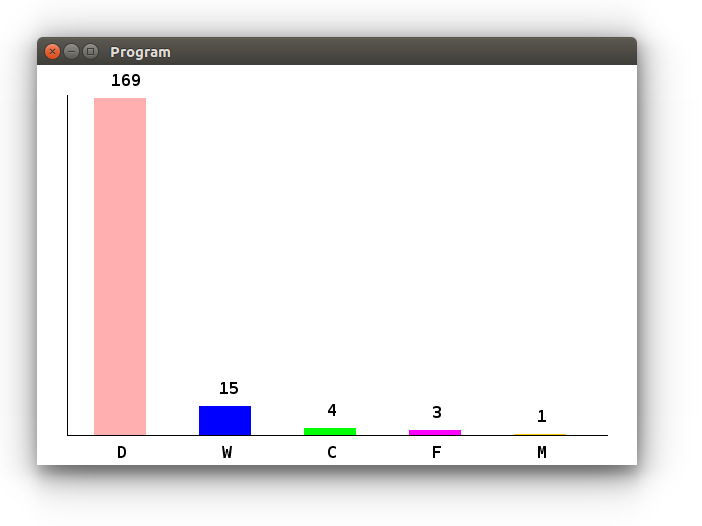
\includegraphics[width=0.9\textwidth]{../img/survey/bar}

\vspace{2em}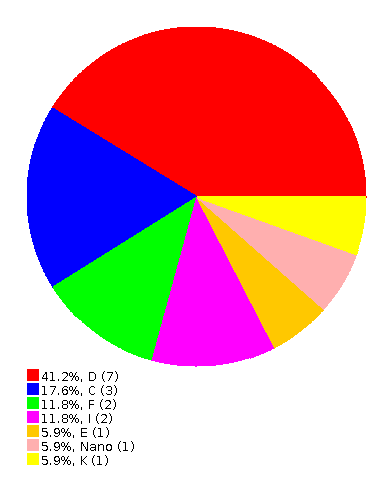
\includegraphics[width=0.7\textwidth]{../img/survey/pie}
\end{minipage}
\end{Slide}


\fi












%!TEX encoding = UTF-8 Unicode
%!TEX root = ../lect-w12.tex

%%%


\Subsection{Repetition: Vad är en algoritm?}
\begin{Slide}{Repetition: Vad är en algoritm? }\SlideFontTiny
\pause En \href{https://sv.wikipedia.org/wiki/Algoritm}{algoritm} är en stegvis beskrivning av hur man löser ett problem. \\ 
Exempel: SWAP, MIN, Registrering, Sökning, Sortering \\
\pause\vspace{0.5em}
Problemlösningsprocessens olika steg (inte nödvändigtvis i denna ordning): 
\begin{itemize}
\item Dela upp problemet i enklare delproblem och sätt samman.
\item Finns redan färdig lösning på (del)problem?
\item Formulera (del)\Emph{problemet} och ange tydligt indata och utdata: \\ exempel MIN: indata: sekvens av heltal; utdata: minsta talet
\item Kom på en \Emph{lösningsidé}: (kan  vara mycket klurigt och svårt) \\ exempel MIN: iterera över talen och håll reda på ''minst hittills''
\item Formulera en \Emph{stegvis beskrivning} som löser problemet: \\ exempel: pseudo-kod med sekvens av instruktioner
\item Implementera en \Emph{körbar lösning} i ''riktig'' kod: \\ exempel: en Scala-metod i en klass eller i ett singelobjekt
\item Har algoritmen acceptabel komplexitet i förhållande till tids- och minneskrav?
\end{itemize}
\pause Det krävs ofta \Emph{kreativitiet} i stegen ovan  -- även i att \Emph{känna igen} problemet!\\
Simpelt exempel: Du stöter på problemet MAX och ser likheten med MIN.\\
\pause\vspace{0.5em}\Emph{Övning}: Diskutera hur du löser detta problem i relation till stegen ovan: \\
\emph{Att räkna antalet förekomster av olika unika ord i en textsträng.} 
\end{Slide}













%!TEX encoding = UTF-8 Unicode
%!TEX root = ../lect-week11.tex

%%%

\ifkompendium\else

\Subsection{Jämföra strängar}

\begin{Slide}{Att jämföra strängar lexikografiskt}\SlideFontSmall
Teckenstandard \href{https://sv.wikipedia.org/wiki/UTF-16}{UTF-16}: Alla stora bokstäver är ''mindre'' än alla små:
\begin{REPLnonum}
scala> Array("hej","Hej","gurka").sorted
\end{REPLnonum}
\pause\vspace{-1.2em}
\begin{REPLnonum}
res0: Array[String] = Array(Hej, gurka, hej)\end{REPLnonum}
\pause
\begin{itemize}
\item Antag att vi vill lösa detta problem ''från scratch'': \\ \Emph{att sortera en sekvens med strängar} 
\item För att göra detta behöver vi lösa dessa delproblemen: 
\begin{itemize}
\item \Emph{att} \Alert{jämföra strängar}
\item \Emph{sökning i sekvenser}
\item \Emph{SWAP} (om på-plats-sortering i förändringsbar sekvens)
\end{itemize}
\item Vad betyder det att två strängar är ''lika''?

\item Vad betyder det att en sträng är ''mindre'' än en annan?
\end{itemize}
\pause {\SlideFontTiny Vi använder här strängjämförelse, sökning och sortering för att illustrera typiska \Emph{imperativa algoritmer}. \Alert{Normalt} använder man \Emph{färdiga lösningar} på dessa problem!}

\end{Slide}

\begin{Slide}{Jämföra strängar: likhet}\SlideFontSmall
Antag att vi inte kan göra \code{s1 == s2} utan bara kan jämföra strängar tecken för tecken, 
t.ex. så här: \code{s1(i) == s2(i)}. Antag också att vi inte har tillgång till annat än metoderna \code{length} och \code{apply} på strängar, samt  \code{while} och variabler av grundtyp. \Emph{Lös problemet att \emph{avgöra om två strängar är lika}.}

\pause
\begin{itemize}
\item Indata: två strängar
\item Utdata: \code{true} om lika annars \code{false}
\end{itemize}
\begin{enumerate}
\item Klura ut din lösningsidé
\item Formulera algoritmen i pseudokod
\item Implementera algoritmen i Scala: \code{def isEqual(s1: String, s2: String): Boolean} = ???
\end{enumerate}
\end{Slide}

\begin{Slide}{Algoritmexempel: stränglikhet, pseudokod}
\begin{Code}
def isEqual(s1: String, s2: String): Boolean = {
  if (/* lika längder */) {
    var foundDiff = false
    var i = /* första index */
    while (!foundDiff && /* i inom indexgräns */) {
      if (/* tecken på plats i är olika */) foundDiff = true
      else i = /* nästa index */
    }
    !foundDiff
  } else false
}
\end{Code}

\pause Detta är en variant av s.k. \Emph{linjärsökning} där vi söker från början i en sekvens till vi hittar det vi söker efter (här söker vi efter tecken som skiljer sig åt). 
\\\pause\vspace{2.5em} Hur ser implementationen i exekverbar Scala ut?
\end{Slide}

\begin{Slide}{Algoritmexempel: stränglikhet, implementation}\SlideFontSmall
\begin{Code}
def isEqual(s1: String, s2: String): Boolean = {
  if (s1.length == s2.length) {
    var foundDiff = false
    var i = 0
    while (!foundDiff && i < s1.length) {
      if (s1(i) != s2(i)) foundDiff = true
      else i += 1
    }
    !foundDiff
  } else false
}
\end{Code}
\pause 
{\SlideFontTiny Fördjupning: jämför ovan med implementationen av \code{String.equals} här:
\href{http://hg.openjdk.java.net/jdk8u/jdk8u60/jdk/file/935758609767/src/share/classes/java/lang/String.java#l976}{hg.openjdk.java.net/jdk8u/jdk8u60/jdk/file/935758609767/src/share/classes/java} \\ och använd \code{timed} nedan och jämför prestanda med \code{isEqual} ovan.\\
Obs! Mät många gånger så att JVM:en optimerar din kod.}
\vspace{-0.25em}\begin{Code}
def timed[T](block: => T): (Double, T) = { 
  val (t, res) = (System.nanoTime, block)
  ((System.nanoTime - t) / 1e9, res) 
}
\end{Code}

\end{Slide}

\begin{Slide}{Algoritmexempel: stränglikhet, prestanda}
\begin{REPL}
scala> val enMiljon = 1000000

scala> val s = Array.fill(enMiljon)('x').mkString

scala> val t = s.updated(enMiljon - 1, 'y')

scala> timed { s == t }
res42: (Double, Boolean) = (3.76459E-4,false)

scala> timed { isEqual(s,t) } 
res43: (Double, Boolean) = (3.31597E-4,false)
\end{REPL}
Ovan är kört efter ''uppvärmning'' på i7-4790K CPU @ 4.00GHz \\
Skillnaden inom mätfelmarginalen!
\end{Slide}



\begin{Slide}{Jämföra strängar: ''mindre än''}\SlideFontSmall
Med \code{s1 < s2} menar vi att strängen s1 ska sorteras före strängen s2 enligt hur de enskilda tecknen är ordnade med uttrycket \code{s1(i) < s2(i)}. \\
Antag också att vi inte har tillgång till annat än metoderna \code{length} och \code{apply} på strängar, samt  \code{while} och variabler av grundtyp, samt \code{math.min}
\\\Emph{Lös problemet att \emph{avgöra om en sträng är ''mindre'' än en annan}.}\\
\begin{itemize}
\item Indata: två strängar, s1, s2
\item Utdata: \code{true} om s1 ska sorteras före s2 annars \code{false}
\end{itemize}
\begin{enumerate}
\item Klura ut din lösningsidé
\item Formulera algoritmen i pseudokod
\item Implementera algoritmen i Scala: \code{def isLessThan(s1: String, s2: String): Boolean} = ???
\end{enumerate}
\end{Slide}

\begin{Slide}{Jämföra strängar: ''mindre än''}\SlideFontSmall
Pseudokod:
\begin{Code}
def isLessThan(s1: String, s2: String): Boolean = {
  
  val minLength = /* minimum av längderna på s1 och s2 */
  
  def firstDiff(s1: String, s2: String): Int = 
    /* index för första skillnaden (om de börjar lika: minLength) */

  val diffIndex = firstDiff(s1, s2)
  if (diffIndex == minLength) /* s1 är kortare än s2 */
  else /* tecknet s1(diffIndex) är mindre än tecknet s2(diffIndex) */ 
}
\end{Code}
\end{Slide}

\begin{Slide}{Jämföra strängar: ''mindre än''}\SlideFontSmall
\begin{Code}
def isLessThan(s1: String, s2: String): Boolean = {

  val minLength = math.min(s1.length, s2.length)

  def firstDiff(s1: String, s2: String): Int = {
    var foundDiff = false
    var i = 0
    while (!foundDiff && i < minLength) 
      if (s1(i) != s2(i)) foundDiff = true 
      else i += 1
    i
  }

  val diffIndex = firstDiff(s1, s2)
  if (diffIndex == minLength) s1.length < s2.length
  else s1(diffIndex) < s2(diffIndex)
}
\end{Code}
\end{Slide}

\begin{Slide}{Jämföra strängar i Java}\SlideFontTiny
\begin{itemize}
\item I Java kan man \Alert{inte} jämföra strängar med operatorerna \code{<}, \code{<=}, \code{>}, och \code{>=}

\item Dessutom ger operatorerna \code{==} och \code{!=} \emph{inte} innehålls(o)likhet utan \Alert{referens(o)likhet} \code{:(}

\item Istället \Alert{måste} man i Java använda metoderna \code{equals} och \code{compareTo} 
\\Dessa fungerar även i Scala eftersom strängar i Scala och Java är av samma typ, nämligen \code{java.lang.String}.
\pause
\item \code{s1.compareTo(s2)} ger ett heltal som är:
\begin{itemize}\SlideFontTiny
\item \code{0} om s1 och s2 har samma innehåll
\item \Alert{negativt} om s1 < s2 i lexikografisk mening, alltså s1 ska sorteras \Alert{före}
\item \Emph{positivt} om s1 > s2 i lexikografisk mening, alltså s1 ska sorteras \Emph{efter}
\end{itemize}

\pause
\item Undersök följande:
\begin{REPL}
scala> new String("hej") eq new String("hej") // motsvarar == i Java
scala> "hej".equals("hej")                    // samma som == i Scala
scala> "hej".compareTo("hej")
scala> "hej".compareTo("HEJ")         // alla stora är 'före' alla små
scala> "HEJ".compareTo("hej")
\end{REPL}
\end{itemize}

\href{http://docs.oracle.com/javase/8/docs/api/java/lang/String.html#compareTo-java.lang.String-}{docs.oracle.com/javase/8/docs/api/java/lang/String.html\#compareTo-java.lang.String-}
\end{Slide}


\begin{Slide}{Jämföra strängar i Java: exempel}\SlideFontSmall
Vad skriver detta Java-program ut?
\javainputlisting{../compendium/examples/StringEqTest.java}
\pause
\begin{REPL}
$ javac StringEqTest.java 
$ java StringEqTest 
false
true
0
\end{REPL}
\end{Slide}


\fi












%!TEX encoding = UTF-8 Unicode
%!TEX root = ../lect-week11.tex

%%%

\ifkompendium\else

\Subsection{Jämförelse Scala och Java}
\begin{Slide}{Grundläggande likheter och skillnader}\SlideFontSmall

\begin{itemize}
\item \Emph{Sökning} återkommer i många skepnader: \\ i en datastruktur, vilken det än må vara, vill man ofta kunna \\ \Emph{hitta ett element med en viss egenskap}. 

\pause
Några färdiga linjärsökningar i Scalas standardbibliotek:

\begin{REPL}
scala> Vector("gurka","tomat","broccoli").indexOf("tomat")
res0: Int = 1

scala> Vector("gurka","tomat","broccoli").indexWhere(_.contains("o"))
res1: Int = 1

scala> Vector("gurka","tomat","broccoli").find(_.contains("o"))
res2: Option[String] = Some(tomat)
\end{REPL}

\pause
\item Sökning efter ett visst index i en sekvens:

\begin{itemize}\SlideFontTiny
\item Indata: en sekvens och ett \Emph{sökkriterium}
\item Utdata: index för första eftersökta element, annars -1 
\end{itemize}

\pause
\item Två typiska varianter av sökning i en sekvens:
\begin{itemize}\SlideFontTiny
\item Linjärsökning: börja från början och sök tills ett eftersökt element är funnet
\item Binärsökning: antag sorterad sekvensen; börja i mitten, välj rätt halva ...
\end{itemize}
\end{itemize}
\end{Slide}

\Subsection{Linjärsökning}

\begin{Slide}{Linjärsökning: hitta index för elementet 42}
Skriv pseudokod för:\\ \code{def indexOf42(xs: Vector[Int]): Int = ???}
\pause
\begin{Code}
def indexOf42(xs: Vector[Int]): Int = {
  var i = /* index för första elementet */
  var found = false
  while (!found && /* index inom indexgräns */) {
    if (/* element på plats i är 42 */) found = true 
    else i = /* nästa index */
  }
  if (/* hittat */) i else -1
} 
\end{Code}
\end{Slide}

\begin{Slide}{Linjärsökning: hitta index för elementet 42}
Implementera:\\ \code{def indexOf42(xs: Vector[Int]): Int = ???}
\pause
\begin{Code}
def indexOf42(xs: Vector[Int]): Int = {
  var i = 0
  var found = false
  while (!found && i < xs.length) {
    if (xs(i) == 42) found = true 
    else i += 1
  }
  if (found) i else -1
} 
\end{Code}
\end{Slide}

\begin{Slide}{Linjärsökning: hitta index för elementet x}
Implementera:\\ \code{def indexOf(xs: Vector[Int], x: Int): Int = ???}
\pause
\begin{Code}
def indexOf(xs: Vector[Int], x: Int): Int = {
  var i = 0
  var found = false
  while (!found && i < xs.length) {
    if (xs(i) == x) found = true 
    else i += 1
  }
  if (found) i else -1
} 
\end{Code}
\end{Slide}

\begin{Slide}{Linjärsökning: hitta index för elementet p(x)}\SlideFontSmall
Implementera:\\ \code{def indexWhere(xs: Vector[Int], p: Int => Boolean): Int = ???}
\pause
\begin{Code}
def indexWhere(xs: Vector[Int], p: Int => Boolean): Int = {
  var i = 0
  var found = false
  while (!found && i < xs.length) {
    if (p(xs(i))) found = true 
    else i += 1
  }
  if (found) i else -1
} 
\end{Code}
\end{Slide}

\begin{Slide}{Linjärsökning: generalisera till godtycklig typ}\SlideFontSmall
Implementera:\\ \code{def indexWhere[T](xs: Vector[T], p: T => Boolean): Int = ???}
\pause
\begin{Code}
def indexWhere[T](xs: Vector[T], p: T => Boolean): Int = {
  var i = 0
  var found = false
  while (!found && i < xs.length) {
    if (p(xs(i))) found = true 
    else i += 1
  }
  if (found) i else -1
} 
\end{Code}
\end{Slide}

\begin{Slide}{Linjärsökning: generalisera till godtycklig typ}\SlideFontSmall
Typinferensen fungerar bättre om stegad funktion:\\ 
\code{def indexWhere[T](xs: Vector[T])(p: T => Boolean): Int}
\begin{Code}
def indexWhere[T](xs: Vector[T])(p: T => Boolean): Int = {
  var i = 0
  var found = false
  while (!found && i < xs.length) {
    if (p(xs(i))) found = true 
    else i += 1
  }
  if (found) i else -1
} 
\end{Code}
\end{Slide}


\begin{Slide}{Linjärsökning: generalisera till godtycklig sekvens}\SlideFontSmall
Implementera:\\ \code{def indexWhere[T](xs: Seq[T])(p: T => Boolean): Int = ???}
\pause
\begin{Code}
def indexWhere[T](xs: Seq[T])(p: T => Boolean): Int = {
  var i = 0
  var found = false
  while (!found && i < xs.length) {
    if (p(xs(i))) found = true 
    else i += 1
  }
  if (found) i else -1
} 
\end{Code}
\end{Slide}

\begin{Slide}{Linjärsökning: generalisera till godtycklig sekvens}\SlideFontSmall
Implementera:\\ \code{def find[T](xs: Seq[T])(p: T => Boolean): Option[T] = ???}
\pause
\begin{Code}
def find[T](xs: Seq[T])(p: T => Boolean): Option[T] = {
  var i = 0
  var found = false
  while (!found && i < xs.length) {
    if (p(xs(i))) found = true 
    else i += 1
  }
  if (found) Some(xs(i)) else None
} 
\end{Code}
\end{Slide}

\Subsection{Binärsökning}

\begin{Slide}{Binärsökning: snabbare men kräver sorterad sekvens}
\begin{REPL}[basicstyle=\color{white}\ttfamily\SlideFontSize{6.5}{8}]
scala> val enMiljon = 1000000

scala> val xs = Array.tabulate(enMiljon)(i => i + 1)   // sorterad

scala> xs(enMiljon - 1)
res0: Int = 1000000

scala> timed { xs.indexOf(enMiljon) }        // linjärsökning
res42: (Double, Int) = (0.016622994,999999)

scala> import scala.collection.Searching._  // ger tillgång till metoden search
import scala.collection.Searching._

scala> timed { xs.search(enMiljon) }        // binärsökning
res54: (Double, collection.Searching.SearchResult) = (2.45691E-4,Found(999999))

\end{REPL}
\pause
Citat från scaladoc för \code{search}:\\
''The sequence \Alert{should be sorted} before calling; otherwise, the results are \Alert{undefined.}''
\end{Slide}

\begin{Slide}{Binärsökning: lösningsidé}
\Emph{Problemlösningsidé}: Om sekvensen är sorterad kan vi utnyttja detta för en mer effektiv sökning, genom att jämföra med mittersta värdet och se om det vi söker finns före eller efter detta, och upprepa med ''halverad'' sekvens tills funnet.
\pause
\begin{itemize}\SlideFontSmall
\item \Emph{Indata}: sorterad sekvens av heltal och det eftersökta elementet
\item \Emph{Utdata}: \code{Found(index)} för det eftersökta elementet
\\ om saknas: \code{InsertionPoint(index)}
\pause
\begin{Code}
sealed trait SearchResult {
  def insertionPoint: Int
}

case class Found(foundIndex: Int) extends SearchResult {
  override def insertionPoint = foundIndex
}
  
case class InsertionPoint(insertionPoint: Int) extends SearchResult
\end{Code}
\end{itemize} 
\end{Slide}

\begin{Slide}{Binärsökning: pseudokod, iterativ lösning}
\Emph{Pseudo-kod}: iterativ lösning
\begin{Code}
def binarySearch(xs: Vector[Int])(elem: Int): SearchResult = {
  var found = false
  var (low, high) = (/* lägsta index */, /* högsta index */)
  var mid = /* något startvärde */ 
  while (!found && /* finns fler element kvar */) {
    mid = /* mittpunkten i intervallet (low, high) */
    if (xs(mid) == elem) found = true
    else if (xs(mid) < elem) /* flytta intervallets undre gräns */
    else /* flytta intervallets övre gräns" */
  }
  if (found) Found(mid)
  else InsertionPoint(low)
}
\end{Code}
\end{Slide}



\begin{Slide}{Binärsökning: implementation, iterativ lösning}
\Emph{Implementation}: iterativ lösning
\begin{Code}
def binarySearch(xs: Vector[Int])(elem: Int): SearchResult = {
  var found = false
  var (low, high) = (0, xs.length - 1)
  var mid = -1 
  while (!found && low <= high) {
    mid = (low + high) / 2
    if (xs(mid) == elem) found = true
    else if (xs(mid) < elem) low = mid + 1
    else high = mid - 1 
  }
  if (found) Found(mid) 
  else InsertionPoint(low)
}
\end{Code}
\end{Slide}

\begin{Slide}{Binärsökning: instrumentering av iterativ lösning}
\vspace{-0.5em}
\begin{CodeSmall}
def waitForEnter: Unit = scala.io.StdIn.readLine("")
def show(msg: String): Unit = {println(msg); waitForEnter}

def binarySearch(xs: Vector[Int])(elem: Int): SearchResult = {
  var found = false                         ; show(s"found = $found")
  var (low, high) = (0, xs.length - 1)      ; show(s"(low, high) = ($low, $high)")
  var mid = -1                              ; show(s"mid = $mid")
  while (!found && low <= high) {           ; show(s"while ${!found && low <= high}")
    mid = (low + high) / 2                  ; show(s"mid = $mid")
    if (xs(mid) == elem) {found = true      ; show(s"found = $found")}
    else if (xs(mid) < elem) {low = mid + 1 ; show(s"low = $low")}
    else {high = mid - 1                    ; show(s"high = $high")}
  }
  if (found) Found(mid) 
  else InsertionPoint(low)
}
\end{CodeSmall}
\vspace{-0.5em}
\begin{REPL}[basicstyle=\color{white}\ttfamily\SlideFontSize{6}{7}]
scala> binarySearch(Vector(0,1,2,3,42,5))(42)
found = false
(low, high) = (0, 5)
mid = -1
while true
mid = 2
low = 3
while true
mid = 4
found = true
res0: collection.Searching.SearchResult = Found(4)
\end{REPL}
\end{Slide}

\begin{Slide}{Binärsökning: rekursiv lösning}
\Emph{Fördjupning}: rekursiv lösning
\begin{Code}
def binarySearch(xs: Vector[Int])(elem: Int): SearchResult = {
  def loop(low: Int, high: Int): SearchResult = 
    if (low > high) InsertionPoint(low) 
    else (low + high) / 2 match {
      case mid if xs(mid) == elem => Found(mid)
      case mid if xs(mid) < elem  => loop(mid + 1, high)
      case mid                    => loop(low, mid - 1)
    }
    
  loop(0, xs.length - 1) 
}
\end{Code}
\end{Slide}


\begin{Slide}{Binärsökning: generisk rekursiv lösning}
\Emph{Fördjupning}: iterativ generisk lösning med implicit ordning
\begin{CodeSmall}
def binarySearch[T](xs: Seq[T])(elem: T)(implicit ord: Ordering[T]): SearchResult = {
  import ord._
  def loop(low: Int, high: Int): SearchResult = 
    if (low > high) InsertionPoint(low) 
    else (low + high) / 2 match {
      case mid if xs(mid) == elem => Found(mid)
      case mid if xs(mid) < elem  => loop(mid + 1, high)
      case mid                    => loop(low, mid - 1)
    }
    
  loop(0, xs.length - 1) 
}
\end{CodeSmall}
{\SlideFontSmall För den intresserade:\\Se fördjupningsuppgifter om implicita ordningar i veckans övning.}
\end{Slide}

\begin{Slide}{Tidskomplexitet, sökning}\SlideFontSmall

\Emph{Fördjupning:}\\Algoritmteoretisk analys av sökalgoritmerna ger:
\begin{itemize}
\item Linjärsökning: tiden är proportionell mot $n$, skrivs: $O(n)$ 
\item Binärsökning:  tiden är proportionell mot $\log_2 n$, skrivs: $O(\log n)$
\end{itemize}
\vspace{1em}\pause
Empirisk analys: Vi har en vektor med 1000 element. Vi har mätt tiden för att söka upp ett element många gånger och funnit att det tar ungefär 1 $\mu$s både med linjärsökning och binärsökning. 
\\\vspace{1em}Hur lång tid tar det om vi har fler element i vektorn?\\
\vspace{1em}
\begin{tabular}{rccccc}
       & 1000 & 10 000 & 100000 & 1 000 000 & 10 000 000 \\ \hline
linjärsökning & 1     & 10     & 100     & 1000     & 10 000 \\
binärsökning  & 1     & 1.33   & 1.67    & 2.00     & 2.33
\end{tabular}
\vspace{1em} 

{\SlideFontTiny 

Kurserna: \\
''\Emph{Utvärdering av programvarusystem}'', obl. för D1, studerar detta \Alert{empiriskt}\\
''\Emph{Algoritmer, datastrukturer och komplexitet}'', obl. för D2, studerar detta \Alert{analytiskt}
}
\end{Slide} 


\fi











%!TEX encoding = UTF-8 Unicode
%!TEX root = ../lect-w12.tex

%%%

\Subsection{Sortering}


\begin{Slide}{Sorteringsproblemet}
\Emph{Problem}: Vi har en osorterad sekvens med heltal. Vi vill ordna denna osorterade sekvens i en sorterad sekvens från minst till störst.
\pause

\vspace{2em}
En \emph{generalisering} av problement: \\ \vspace{1em} Vi har många element av godtycklig typ och en \Emph{ordningsrelation} som säger vad vi menar med att ett element är \emph{mindre än} eller \emph{större än eller lika med} ett annat element. \\ \vspace{1em}
Vi vill lösa problemet att ordna elementen i sekvens så att för varje element på plats $i$ så är efterföljande element på plats $i + 1$ större eller lika med elementet på plats $i$.

\end{Slide}

\begin{Slide}{Två enkla sporteringsalgoritmer: \\ Insättningssortering \& Urvalssortering}
\begin{itemize}
\item Insättningssortering \Emph{lösningsidé}: Ta ett element i taget från den osorterade listan och \Alert{sätt in} det på \Alert{rätt plats} i den sorterade listan och upprepa till det inte finns fler osorterade element.
\pause
\item Urvalsssortering \Emph{lösningsidé}: \Alert{Välj ut} det minsta kvarvarande elementet i den osorterade listan och placera det \Alert{sist} i den sorterade listan och upprepa till det inte finns fler osorterade element.
\end{itemize}
\end{Slide}



\begin{Slide}{Tidskomplexitet, sortering, medeltal}
\begin{tabular}{ll}
Urvalssortering, insättningssortering: & $O(n^2)$ \\
''Bra'' metoder, tex Quicksort, Timsort:  & $O(n\log n)$
\end{tabular}

\vspace{1em}\footnotesize
Vi har en vektor med 1000 element. Vi har mätt tiden för att sortera elementen många gånger och funnit att det tar ungefär 1 ms både med urvalssortering (eller någon annan ''dålig'' metod) och en ''bra'' metod. Hur lång tid tar det om vi har fler element i vektorn?

\vspace{1em}
\begin{tabular}{rccccc}
       & 1,000 & 10,000 & 100,000 & 1,000,000 & 10,000,000 \\ \hline
dålig  & 1     & 100    & $10^4$  & $10^6$   & $10^8$ \\
bra    & 1     & 13.3   & 167     & 2000     & 23000
\end{tabular}
\end{Slide}

\begin{Slide}{Bogo sort}
\begin{Code}
def bogoSort(xs: Vector[Int]) = {
  var result = xs
  while(result != result.sorted) {
    result = scala.util.Random.shuffle(result)
  }
  result
}
\end{Code}
När blir denna färdig? \pause \\
\url{https://en.wikipedia.org/wiki/Bogosort}\\
Antal jämförelser i medeltal vid många mätningar: $ O(n \cdot n!) $
\end{Slide}





\begin{Slide}{Det finns många olika sorteringsalgoritmer}
\begin{itemize}
\item Visualisering av 15 olika sorteringsalgoritmer på 6 min:\\{\SlideFontSmall\url{https://www.youtube.com/watch?v=kPRA0W1kECg}}
\item Olika sorteringsalgoritmer har olika tids- \& minneskomplexitet: i bästa fall, i värsta fall, i medeltal, för nästan sorterad, etc.
\\{\SlideFontSmall\url{https://en.wikipedia.org/wiki/Sorting_algorithm}}
\item Olika sorteringsalgoritmer lämpar sig olika väl för parallellisering på många kärnor.
\end{itemize}
\end{Slide}




\begin{Slide}{Insättnings- och urvalssortering}
\Emph{Insertion sort}
\begin{itemize}
\item Wikipedia:\\
{\SlideFontSmall\url{https://sv.wikipedia.org/wiki/Insättningssortering}}
{\SlideFontSmall\url{https://en.wikipedia.org/wiki/Insertion_sort}}

\item AlgoRythmics: Insert-sort with Romanian folk dance\\
{\SlideFontSmall\url{https://www.youtube.com/watch?v=ROalU379l3U}}
\end{itemize}

\vspace{2em}
\Emph{Selection sort}

\begin{itemize}
\item Wikipedia:\\ 
{\SlideFontSmall\url{https://sv.wikipedia.org/wiki/Urvalssortering}}\\
{\SlideFontSmall\url{https://en.wikipedia.org/wiki/Selection_sort}}

\item AlgoRythmics: Select-sort with Gypsy folk dance \\ 
{\SlideFontSmall\url{https://www.youtube.com/watch?v=Ns4TPTC8whw}}
\end{itemize}
\end{Slide}




\begin{Slide}{Sortera till ny vektor med insättningssortering: pseudo-kod}

{\SlideFontSmall Det är nog lättare att förstå \Emph{insertion sort} om man sorterar till en ny vektor. \\ Vi ska sedan se hur man sorterar ''på plats'' \Eng{in place} i en  array.\\} \vspace{1em}
\Emph{Indata}: en osorterad vektor med heltal \\
\Emph{Utdata}: en ny, sorterad vektor med heltal
\begin{Code}
def insertionSort(xs: Vector[Int]): Vector[Int] = {
  val sorted = /* tom ArrayBuffer */
  for (/* alla element i xs */) {
     /* linjärsök rätt position i sorted */
     /* sätt in element på rätt plats i sorted */
  }
  sorted.toVector
}
\end{Code}
\end{Slide}


\begin{Slide}{Sortera till ny vektor med insättningssortering: implementation i Scala}
\begin{Code}
def insertionSort(xs: Vector[Int]): Vector[Int] = {
  val sorted = scala.collection.mutable.ArrayBuffer.empty[Int]
  for (elem <- xs) {
     // linjärsök rätt position i sorted:
     var pos = 0
     while (pos < sorted.length && sorted(pos) < elem) {
       pos += 1
     }
     // sätt in element på rätt plats i sorted:
     sorted.insert(pos, elem)
  }
  sorted.toVector
}
\end{Code}
\end{Slide}

\begin{Slide}{Sortera till ny vektor med insättningssortering: implementation i Java med foreach-sats}
\SlideFontTiny\vspace{-0.5em}
\begin{Code}[language=Java]
import java.util.ArrayList;

public class JSort {
    public static ArrayList<Integer> insertionSort(ArrayList<Integer> xs) {
        ArrayList<Integer> sorted = new ArrayList<Integer>();
        for (int elem : xs) {
            // linjärsök rätt position i sorted:
            int pos = 0;
            while (pos < sorted.size() && sorted.get(pos) < elem) {
                pos++;
            }
            // sätt in element på rätt plats i sorted:
            sorted.add(pos, elem);
        }
        return sorted;
    }
}
\end{Code}
\vspace{-0.3em}
\href{http://stackoverflow.com/questions/85190/how-does-the-java-for-each-loop-work}{ stackoverflow.com/questions/85190/how-does-the-java-for-each-loop-work}

Javasamlingar måste ''wrappa'' primitiva \jcode{int} i klassen \code{Integer} (mer om detta senare)
\end{Slide}

\begin{Slide}{Sortera till ny vektor med urvalssortering: pseudo-kod}

{\SlideFontSmall Det är nog lättare att förstå \Emph{selection sort} om man sorterar till en ny vektor. \\ Vi ska sedan se hur man sorterar ''på plats'' \Eng{in place} i en  array.\\} \vspace{1em}
\Emph{Indata}: en osorterad vektor med heltal \\
\Emph{Utdata}: en sorterad vektor med heltal
\begin{Code}
def selectionSort(xs: Vector[Int]): Vector[Int] = {
  val unsorted = xs.toBuffer
  val sorted = scala.collection.mutable.ArrayBuffer.empty[Int]
  while (/* unsorted inte är tom */) {
    var indexOfMin = /* index för minsta element i unsorted */
    /* flytta elementet unsorted(indexOfMin) till sist i sorted */
  }
}
\end{Code}
\end{Slide}

\begin{Slide}{Sortera till ny vektor med urvalssortering: implementation i Scala}
\SlideFontTiny\vspace{-0.5em}
\begin{Code}
def selectionSort(xs: Vector[Int]): Vector[Int] = {
  val unsorted = xs.toBuffer
  val sorted = scala.collection.mutable.ArrayBuffer.empty[Int]
  while (unsorted.nonEmpty) {
    var indexOfMin = 0
    // index för minsta element i unsorted:
    for (i <- 1 until unsorted.length) {
      if (unsorted(i) < unsorted(indexOfMin)) indexOfMin = i
    }
    val elem = unsorted.remove(indexOfMin)  // ta bort ur unsorted
    sorted.append(elem)  // lägg sist i sekvensen med sorterade
  }
  sorted.toVector
}
\end{Code}
\pause
\begin{itemize}
\item Funkar tom sekvens?
\item Funkar en sekvens med ett element?
\item Funkar det för osorterad sekvens med (minst) två element?
\item Vad händer om sekvensen är sorterad?
\end{itemize}
\end{Slide}

\begin{Slide}{Sortera till ny vektor med urvalssortering: implementation i Java}
\begin{Code}[language=Java]
public static ArrayList<Integer> selectionSort(ArrayList<Integer> unsorted) {
    ArrayList<Integer> sorted = new ArrayList<Integer>();
    while (unsorted.size() > 0) {
        int indexOfMin = 0;
        // index för minsta element i unsorted:
        for (int i = 1; i < unsorted.size(); i++) {
            if (unsorted.get(i) < unsorted.get(indexOfMin)) {
                indexOfMin = i;
            }
        }
        int elem = unsorted.remove(indexOfMin);  // ta bort ur unsorted
        sorted.add(elem);  // lägg sist i sekvensen med sorterade
    }
    return sorted;
}
\end{Code}
OBS! Ovan algoritm ''\Alert{förstör}'' innehållet i inparametern! \\ Hur förhindra det?
\end{Slide}

\begin{Slide}{Sortera till ny vektor med urvalssortering: implementation i Java}
\begin{Code}[language=Java]
public static ArrayList<Integer> selectionSort(ArrayList<Integer> xs) {
    ArrayList<Integer> unsorted = new ArrayList<Integer>(xs); //ref copy
    ArrayList<Integer> sorted = new ArrayList<Integer>();
    while (unsorted.size() > 0) {
        int indexOfMin = 0;
        // index för minsta element i unsorted:
        for (int i = 1; i < unsorted.size(); i++) {
            if (unsorted.get(i) < unsorted.get(indexOfMin)) {
                indexOfMin = i;
            }
        }
        int x = unsorted.remove(indexOfMin);  // ta bort ur unsorted
        sorted.add(x);  // lägg sist i sekvensen med sorterade
    }
    return sorted;
}
\end{Code}
\end{Slide}

\begin{Slide}{Urvalssortering på plats: pseudo-kod}
\Emph{Indata:} en array med heltal\\
\Emph{Utdata:} samma array, men nu sorterad\\

\begin{Code}
def selectionSortInPlace(xs: Array[Int]): Unit = {
  def minIndex(fromIndex: Int): Int = {
    /* index för minsta element från fromIndex  */
  }

  for (i <- /* från första till NÄST sista index */) {
    /* byt plats mellan xs[i] och xs[minIndex(i)] */
  }
}
\end{Code}
\pause
Se animering här: \href{https://sv.wikipedia.org/wiki/Urvalssortering}{Urvalssortering på Wikipedia}
\end{Slide}

\begin{Slide}{Urvalssortering på plats: implementation i Scala}\SlideFontSmall
\vspace{-0.25em}
\Emph{Indata:} en array med heltal\\
\Emph{Utdata:} samma array, men nu sorterad\\

\begin{Code}[numberstyle=\ttfamily\SlideFontSize{6}{7.5},numbers=left]
def selectionSortInPlace(xs: Array[Int]): Unit = {
  def minIndex(fromIndex: Int): Int = {
    var result = fromIndex
    for (i <- fromIndex + 1 until xs.length) {
      if (xs(i) < xs(result)) result = i
    }
    result
  }

  def swap(i: Int, j: Int): Unit = {
    val temp = xs(i)
    xs(i) = xs(j)
    xs(j) = temp
  }

  for (i <- 0 until xs.length - 1) { // till NÄST sista
    swap(i, minIndex(i))
  }
}
\end{Code}
\end{Slide}

\begin{Slide}{Selection sort, in place, Java}\SlideFontTiny
Om man ''slår ihop'' del-lösningarna minIndex och swap så kan man skriva detta lite kortare och utnyttja att variablen min nedan kan användas i stället för temp.  \\
OBS! Det är viktigare att koden är lättläst än att den är kort och koden optimeras åt oss av kompilatorn och/eller JVM så extra variabler och funktionsanrop är sällan problem.
\begin{Code}[language=Java,basicstyle=\ttfamily\SlideFontSize{6}{7.5},numberstyle=\ttfamily\SlideFontSize{6}{8}, numbers=left]
public static void selectionSortInPlace(int[] xs) {
    for (int i = 0; i < xs.length - 1; i++) {
        int min = Integer.MAX_VALUE;
        int minIndex = -1;
        for (int k = i; k < xs.length; k++) {
            if (xs[k] < min) {
                min = xs[k];
                minIndex = k;
            }
        }
        xs[minIndex] = xs[i];
        xs[i] = min;
    }
}
\end{Code}


\pause Det finns ett specialfall som kommer krascha denna implementation. Vilket?
\pause\\\jcode|new int[]{Integer.MAX_VALUE, Integer.MAX_VALUE}|
\end{Slide}

\begin{Slide}{Insättningssortering på plats -- pseudo-kod}
\Emph{Indata:} en array med heltal\\
\Emph{Utdata:} samma array, men nu sorterad\\
\begin{Code}
def insertionSortInPlace(xs: Array[Int]): Unit = {
  for (i <- 1 until xs.length) {  //från ANDRA till sista
    var j = i
    while (j > 0 && xs(j - 1) > xs(j)) {
      /* byt plats på xs(j) och xs(j - 1) */
      j -= 1;  // stega bakåt
    }
  }
}
\end{Code}
\pause
Se animering här: \href{https://sv.wikipedia.org/wiki/Ins\%C3\%A4ttningssortering}{Insättningssortering på wikipedia}\\
Gå igenom alla specialfall och kolla så att detta fungerar!
\end{Slide}

\begin{Slide}{Insertion sort, in place, Scala}
\begin{Code}
def insertionSortInPlaceSwap(xs: Array[Int]): Unit = {
  def swap(i: Int, j: Int): Unit = {
    val temp = xs(i)
    xs(i) = xs(j)
    xs(j) = temp
  }
  for (i <- 1 until xs.length) {  //från ANDRA till sista
    var j = i
    while (j > 0 && xs(j - 1) > xs(j)) {
      swap(j, j - 1)
      j -= 1;  // stega bakåt
    }
  }
}
\end{Code}
\end{Slide}


\begin{Slide}{Insertion sort, in place, with swap, Java}
Vi kan tyvärr inte ha lokala funktioner i Java.
\begin{Code}[language=Java]
private void swap(int[] xs, int a, int b) {
    int temp = xs[a];
    xs[a] = xs[b];
    xs[b] = temp;
}

public void insertionSortInPlaceSwap(int[] xs) {
    for (int i = 1; i < xs.length; i++) {
        int j = i;
        while (j > 0 && xs[j - 1] > xs[j]) {
            swap(xs, j, j - 1);
            j = j - 1;
        }
    }
}
\end{Code}
\end{Slide}

\begin{Slide}{Insertion sort, in place, kortare implementation}
Kortare! Men kanske inte mer lättläst?
\begin{Code}[language=Java]
    public void insertionSortInPlace(int[] xs) {
        for (int i = 1; i < xs.length; i++) {
            int current = xs[i];
            int j = i;
            while (j > 0 && xs[j - 1] > current) {
                xs[j] = xs[j - 1];
                j--;
            }
            xs[j] = current;
        }
    }
\end{Code}

\end{Slide}




\begin{Slide}{Sortera samlingar med godtyckligt ordningspredikat}
\begin{Code}
def sortWith(xs: Vector[Int])(lt: (Int, Int) => Boolean ): Vector[Int] = {
  val sorted = scala.collection.mutable.ArrayBuffer.empty[Int]
  for (elem <- xs) {  // insertion sort using lt as "less than"
     var pos = 0
     while (pos < sorted.length && lt(sorted(pos), elem)) {
       pos += 1
     }
     sorted.insert(pos, elem)
  }
  sorted.toVector
}
\end{Code}
\pause
\begin{REPL}
scala> val xs = Vector(1,2,1,2,12,42,1)
xs: scala.collection.immutable.Vector[Int] = Vector(1, 2, 1, 2, 12, 42, 1)

scala> sortWith(xs)(_ < _)
res0: Vector[Int] = Vector(1, 1, 1, 2, 2, 12, 42)

scala> sortWith(xs)(_ > _)
res1: Vector[Int] = Vector(42, 12, 2, 2, 1, 1, 1)
\end{REPL}
\end{Slide}


\begin{Slide}{Fördjupning: Sortera samlingar av godtycklig typ}
\vspace{-0.25em}
\begin{Code}
def sortWith[T](xs: Vector[T])(lt: (T, T) => Boolean ): Vector[T] = {
  val sorted = scala.collection.mutable.ArrayBuffer.empty[T]
  for (elem <- xs) {
     var pos = 0
     while (pos < sorted.length && lt(sorted(pos), elem)) {
       pos += 1
     }
     sorted.insert(pos, elem)
  }
  sorted.toVector
}
\end{Code}
\pause\vspace{-0.25em}
\begin{REPL}
scala> case class Gurka(namn: String, vikt: Int)

scala> val xs = Vector(Gurka("a", 100), Gurka("b", 50), Gurka("c", 100))

scala> sortWith(xs)(_.vikt > _.vikt)
res0: Vector[Gurka] = Vector(Gurka(c,100), Gurka(a,100), Gurka(b,50))

scala> sortWith(xs)(_.vikt >= _.vikt)
res1: Vector[Gurka] = Vector(Gurka(a,100), Gurka(c,100), Gurka(b,50))
\end{REPL}
\end{Slide}


\begin{Slide}{Vad menas med att en sorteringsalgoritm är stabil?}
En sorteringsalgoritm är \Emph{stabil} om \Alert{ordningen} mellan element som anses \Emph{lika} enligt sorteringsordningsrelationen \Alert{bevaras}.\\\vspace{1em}
Fördjupning:
\href{https://en.wikipedia.org/wiki/Sorting_algorithm#Stability}
{en.wikipedia.org/wiki/Sorting\_algorithm\#Stability}
\end{Slide}

\begin{Slide}{Sortera samlingar med inbyggda sortBy och sortWith}
\begin{REPL}
scala> case class Gurka(namn: String, vikt: Int)
defined class Gurka

scala> val xs = Vector(Gurka("a", 100), Gurka("b", 50), Gurka("c", 100))

scala> xs.sortBy(_.vikt)
res0: scala.collection.immutable.Vector[Gurka] =
        Vector(Gurka(b,50), Gurka(a,100), Gurka(c,100))

scala> xs sortWith (_.vikt > _.vikt)
res1: scala.collection.immutable.Vector[Gurka] =
        Vector(Gurka(a,100), Gurka(c,100), Gurka(b,50))

\end{REPL}
\end{Slide}



\begin{Slide}{Fördjupning: sortera samlingar implicit ordning}
\begin{REPL}
scala> case class Gurka(namn: String, vikt: Int)
defined class Gurka

scala> val xs = Vector(Gurka("a", 100), Gurka("b", 50), Gurka("c", 100))

scala> xs.sorted
<console>:15: error: No implicit Ordering defined for Gurka.
       xs.sorted
          ^
\end{REPL}
\pause
Detta kan fixas genom att tillhandahålla en \Emph{implicit} ordning för \code{Gurka}:
\begin{Code}
implicit object minGurkOrdning extends Ordering[Gurka] {
  def compare(x: Gurka, y: Gurka): Int =
    if (x == y) 0
    else if (x.vikt < y.vikt) -1
    else 1
}
\end{Code}
\end{Slide}


\begin{Slide}{Fördjupning: sortera samlingar implicit ordning}
\begin{REPL}
scala> case class Gurka(namn: String, vikt: Int)
defined class Gurka

scala> val xs = Vector(Gurka("a", 100), Gurka("b", 50), Gurka("c", 100))

scala> implicit object minGurkOrdning extends Ordering[Gurka] {
         def compare(x: Gurka, y: Gurka): Int =
           if (x == y) 0
           else if (x.vikt < y.vikt) -1
           else 1
       }

scala> xs.sorted
res0: scala.collection.immutable.Vector[Gurka] =
        Vector(Gurka(b,50), Gurka(a,100), Gurka(c,100))
\end{REPL}
{\SlideFontTiny Se exempel på olika bekvämare sätt att definiera en ordning för dina egna typer: 
\url{https://stackoverflow.com/questions/19345030/easy-idiomatic-way-to-define-ordering-for-a-simple-case-class}}
\end{Slide}


\begin{Slide}{Vad kommer (inte) på tentan?}
Detta \Emph{kan} komma på tentan:
\begin{itemize}
\item Använda färdiga söknings- och sorteringsfunktioner på samlingar av specifik typ
\item Implementera egen linjärsökning i samlingar av specifik typ
\item Implementera egen binärsökning i samlingar av specifik typ
\item Implementera egen sortering till ny samling av specifik typ (du får själv välja algoritm, lämpligen insättnings- eller urvalssortering)

\end{itemize}
Detta kommer \Alert{inte} på tentan:
\begin{itemize}
\item Implementera generisk sökning
\item Implementera generisk sortering
\item Implementera sortering ''på plats''
\item Bogo sort
\end{itemize}
\end{Slide}


\Lecture{13}{Tentaträning, Projekt}
%!TEX encoding = UTF-8 Unicode
%!TEX root = ../lect-week14.tex

%%%

\Subsection{Tentatips}
\begin{Slide}{Före tentan:}\SlideFontSmall
\begin{enumerate}
\item Repetera övningar och labbar i kompendiet.
\item Läs igenom föreläsningsanteckningar.
\item Studera \Emph{snabbref} \Alert{mycket noga} så att du vet vad som är givet och var det står, så att du kan hitta det du behöver snabbt.
\item Skapa och \Emph{memorera} en personlig \Emph{checklista} med programmeringsfel du brukar göra, som även inkluderar småfel, så som glömda parenteser och semikolon, och annat som en kompilator/IDE normalt hittar.
\item Tänk igenom hur du ska disponera dina 5 timmar på tentan.
\item Gör minst en extenta som om det vore \Alert{skarpt läge}:
\begin{enumerate}\SlideFontTiny
\item Avsätt 5 ostörda timmar (stäng av telefon, dator etc).
\item Inga hjälpmedel. Bara snabbref.
\item Förbered dryck och tilltugg.
\end{enumerate}
\end{enumerate}
\end{Slide}

\begin{Slide}{På tentan:} \SlideFontTiny
\begin{enumerate}
\item Läs igenom \Alert{hela} tentan först. \\ \Emph{Varför?} Förstå helheten. Delarna hänger ihop.
\item Notera och begrunda specifika begrepp och definitioner. \\ \Emph{Varför?} Begreppen är avgörande för förståelsen av uppgiften.
\item Notera förenklingar, antaganden och specialfall. \\ \Emph{Varför?} Uppgiften blir mkt enklare om du inte behöver hantera dessa.
\item \Alert{Fråga} tentamensansvarig om du inte förstår uppgiften -- speciellt om det finns misstänkta felaktigheter eller förmodat oavsiktliga oklarheter. \\ \Emph{Varför?} Det är inte lätt att konstruera en ''perfekt'' tenta. \\ Du får fråga vad du vill, men det är inte säkert du får svar :)
\item Läs specifikationskommentarerna och metodsignaturerna i alla givna klass-specifikationer \Alert{mycket noga}. \\ \Emph{Varför?} Det är ett vanligt misstag att förbise de ledtrådar som ges där.
\item Återskapa din memorerade personliga checklista för vanliga fel som du brukar göra och avsätt tid till att gå igenom den på tentan. Varje fix plockar poäng!
\item Lämna in ett försök även om du vet att lösningen inte är fullständig. Det gäller att ''plocka poäng'' på så mycket som möjligt. En dålig lösning kan ändå ge poäng.

\item Om du har svårigheter kan det bli kamp mot klockan. Försök hålla huvudet kallt och prioritera utifrån var du kan plocka flest poäng. Ge inte upp! Ta en kort äta-dricka-paus för att få mer energi!

\end{enumerate}
\end{Slide}

\ifkompendium\else

\begin{Slide}{Planeringstips}\SlideFontTiny
Exempel på saker som du kan lägga in tid för i din julpluggkalender:
\begin{enumerate}
\item Välja ut övningar att repetera
\item Repetera övning X, Y, Z, ... Både läsa och skriva kod. Fundera på typ och värde.
\item Välja ut labbar att repetera
\item Repetera labb X, Y, Z, ... Lär dig ''trick'' och ''mönster''.
\item Träna på att skriva program med papper och penna
\item Göra checklista med vanliga fel och misstag som du brukar göra
\item Det finns inte så många Scala-extentor, men du kan använda Java-extentor som om de vore i skarpt läge; du kan med fördel lösa vissa delar i Scala och vissa delar i Java beroende på vad du behöver träna på

\item Läsa igenom de extentor i Scala och Java som du inte väljer att göra som om det vore skarpt läge och studera uppgifterna och lösningarna och notera generella mönster och typiska trick
\end{enumerate}
\end{Slide}

\begin{Slide}{Tentans struktur}
\begin{itemize}
\item Del A 20\%:\\\Emph{Läsa uttryck} där du ska \Alert{ange typ och värde}
\begin{itemize}\SlideFontTiny
\item Testar förståelse av variabler, uttryck, samlingar, algoritmer, arv, etc.
\item Det är bra/nödvändigt att skriva ner delsteg och variablers värden, då det kan vara svårt att tänka ut svaren direkt i huvudet.
\item Ev. ''rättningströskel'': \textit{Om du på del A erhåller färre poäng än vad som krävs för att nå upp till en bestämd ''rättningströskel'', kan din tentamen komma att underkännas utan att del B bedöms.}
\end{itemize}


\item Del B 80\%:\\\Emph{Skriva kod} som uppfyller \Alert{krav och designspecifikation}
\begin{itemize}\SlideFontTiny
\item Testar att du själv kan skapa kod med delar som samverkar
\item Testar förmåga att gå från indata-utdata till algoritm \\
 givet: ledtrådar, design, ev. skiss på lösning, ev. pseudokod etc.
\item En uppgift ska besvaras i Java, men den testar mer än bara Java-kompetens. Det är bättre att svara i Scala-liknande Java om du är osäker på Java än att inte lämna in alls.
\end{itemize}
\item Blanka inlämningar ger 0 poäng; det är alltid bättre att försöka än att lämna in blankt.
\end{itemize}
\end{Slide}


\begin{Slide}{Vad kommer på tentan? (1 av 3)}\SlideFontTiny
\hspace{-1em}\begin{minipage}{1.0\textwidth}
Allmänt:
\begin{itemize}\SlideFontTiny
\item Begrepp som är ''fördjupning'' krävs ej på tentan (men ökar förståelse)
\item Ok om du väljer en enklare lösning med basala begrepp som fungerar bra, \\i stället för en kortare/elegantare/mer avancerad lösning
\item Dessa moduler ingår ej på tentan: ''Trådar, webb'', ''Design, api''
\end{itemize}

\vspace{1em}\begin{tabular}{l | l | l}
\textbf{Modul} & \textit{Ingår t.ex.}& \textit{Avgränsning} (ej krav; ok anv. om lämpl.)\\\hline
Introduktion & uttryck, aritmetik, slumptal, & kan ha nytta av deMorgan men ej krav\\
             & strängar, typer, Unit     \\
             & skillnad mellan heltal \& flyttal & Float, Byte, Short\\
             & variabler, for, while, if & hex-literaler, backticks\\
\hline
Kodstrukturer & iterering, SWAP, SUM, MIN/MAX & import, paketnamn\\
              & loopar, Range, sats vs uttryck & ok att välja vilken loop du tycker passar\\
              & namn, synlighet, skuggning & scaladoc, javadoc, jar \\
\hline
Funktioner,   & definiera, anropa, parameter& skapa egen kontrollstruktur\\
objekt        & returtyp, namnarop, defaultarg & stegad funktion, rekursion\\
              & punktnotation, objekt vs static & lazy val\\
              & map/foreach med egen funktion & \\
              & anonyma funktioner (lambda)  & \\

\end{tabular}
\end{minipage}
\end{Slide}


\begin{Slide}{Vad kommer på tentan? (2 av 3)}\SlideFontTiny
\hspace{-2em}\begin{minipage}{1.0\textwidth}
\begin{tabular}{l | l | l}
\textbf{Modul} & \textit{Ingår t.ex.}& \textit{Avgränsning} (ej krav; ok anv. om lämpl.)\\\hline
Datastrukt. & attribut, medlem, metod, klass & isInstanceOf (anv. match istället) \\
            & tupler, Vector, Set, Map & List (oftast Vector istället)\\
            & Source.fromFile          & java.nio.file \\
\hline
Sekvensalg. &  skapa ny samling från befintlig &  \\
            &  registrering, Scanner, ArrayBuffer & StringBuilder\\
            &  uppdatera Array, ArrayBuffer, Vector & \\
            &  slumptalsfrö, scala.util.Random  &  \\
\hline

Klasser     &  new, this, synlighet  & null \\
            &  inkapsling, accessregler, private  & private[this] \\
            &  klassparameter, fabriksmetod  & \\
            &  class vs case class    & \\
            &  referenslikhet vs innehållslikhet    & \\
            &  föränderlig vs oföränderlig klass & \\
\hline
Arv         &  bastyp, subtyp, trait, extends  & \\
            &  överskuggning,                  & inmixning, \\
            &  Any, AnyVal, AnyRef, Object     & Null, Nothing\\
            &  accessregler vid arv, protected & final\\
            &  abstract class, case object     & \\

\end{tabular}
\end{minipage}
\end{Slide}


\begin{Slide}{Vad kommer på tentan? (3 av 3)}\SlideFontTiny
\hspace{-2em}\begin{minipage}{1.0\textwidth}
\begin{tabular}{l | l | l}
\textbf{Modul} & \textit{Ingår t.ex.}& \textit{Avgränsning} (ej krav; ok anv. om lämpl.)\\\hline

Mönster     & match, Option, Try & try catch, unapply\\
            & flatten, sealed            & flatMap, partiella funktioner\\
            & enkel equals utan arv     & hashcode, fullständig equals   \\
            & wildcard-mönster  & variabelbindn. i mönster, sekvensmönster\\
\hline

Matriser,     & indexering i nästlade strukturer & \\
typparametrar & nästlad for-sats  & \\
              & matriser i Java med array  & \\
              & använda generiska strukturer & skapa generiska strukturer\\
\hline

Sök, sortera & linjärsökning, binärsökning & algoritmisk komplexitet\\
            & compareTo, strängjämförelse & Ordering, Ordered\\
            & insättningssortering & räcker kunna en valfri sortering \\
\hline


Scala/Java & översätta enkel Java/Scala & try catch i Java \\
           & implemenetera Java-klass     &  arv i Java med super vid konstr.\\
           & grundläggande syntaxskillnader & \\
           & ArrayList vs ArrayBuffer & java.util.\{List, Set\}\\
           & Autoboxing vid ArrayList<Integer> & \\
\multicolumn{3}{c}{OBS! Java-övningar finns även här och där i andra moduler}\\
\hline

\end{tabular}
\end{minipage}
\end{Slide}



\begin{Slide}{Några tumregler/tips vid val av abstraktion}\SlideFontSmall
Ofta ger tentan en specifik design, men du kan ha stor nytta av egna abstraktioner, speciellt \Emph{lokala funktioner} för att göra enklare dellösningar!

\pause\vspace{1em}Om du skulle behöva samla både attribut och metoder utöver givna specifikationer:
Singelobjekt, case-klass, klass, trait eller abstrakt klass?
\begin{itemize}\SlideFontTiny
\item Använd \code{object} om du behöver samla metoder (och variabler) i en modul som bara finns i en upplaga. Du får lokal namnrymd och punktnotation på köpet.
\item Använd en \code{case class} om du har \Emph{oföränderlig data}. Du får då även innehållslikhet, möjlighet till mönstermatchning, etc. på köpet!
\item Behöver du \Alert{föränderligt tillstånd} använd en vanlig \code{class}.\\ Det normala är att tillståndet (alla attribut) är \code{private} eller \code{protected} och att all uppdatering och avläsning av tillståndet sker indirekt genom metoder (getters/setters/...).
\item Behöver du en abstrakt bastyp utan konstruktorparametrar använd en \code{trait}. \\(Du får inmixningsmöjlighet med \code{with} på köpet. Inmixning kommer ej på tenta.)
\item Behöver du en abstrakt bastyp med konstruktorparametrar använd en \code{abstract class}. (Går dock ej att använda vid inmixning med \code{with}.)
\end{itemize}
\end{Slide}


\begin{Slide}{Tips om hur man läser en specifikation}\SlideFontSmall
När du läser en specifikation av en klass, en trait, eller ett singelobjekt:
\begin{itemize}
\item Tänk igenom vilket ansvar olika delar av koden har
\item Vad håller klassen reda på? \\$\rightarrow$ Ledtrådar till attribut
\item Vad ska klassen göra/räkna ut? \\$\rightarrow$ Ledtrådar till metoder och deras algoritm
\item Vilka andra klasser har nytta av denna metod? \\$\rightarrow$ Ledtrådar till hur klasserna samverkar för att lösa uppgiften
\end{itemize}
Rita gärna en bild med ett specifikt exempel på vilken data som olika instanser håller reda på och fundera på hur data skapas/beräknas/förändras
\end{Slide}


\begin{Slide}{Tips om val av samling}\SlideFontSmall

Generellt: Det är ofta enklare med oföränderliga samlingar med oföränderliga element och skapa nya samlingar vid förändring. Men ibland blir det enklare om man har föränderliga samlingar.

\begin{itemize}
\item Behöver du hantera värden \code{x} av t.ex. typen String med \Emph{heltalsindex}?
\begin{itemize}\SlideFontTiny
\item Om du klarar dig utan förändring av innehållet:\\ \code{ val xs: Vector[String]}
\item Om du behöver ändra innehåll men \Alert{inte} antal element: \\ \code{ val xs: Array[String]}
\item Om du behöver ändra innehåll \Alert{och} antal element:
\\ \code{ var xs: Vector[String] } (se metoden \code{patch}) eller \\ \code{ val xs: ArrayBuffer[String]} (har metoden \code{insert})
\end{itemize}

\item Behöver du hantera värden \code{x} som ska vara unika?
\begin{itemize}\SlideFontTiny
\item Oföränderlig: \code{  val xs: Set[String] }
\item Förändringsbar: \code{val xs: scala.collection.mutable.Set[String]}
\end{itemize}

\item Behöver du leta upp värden \code{x:Int} utifrån en nyckel av t.ex. String?
\begin{itemize}\SlideFontTiny
\item Oföränderlig: \code{   val xs: Map[String, Int] }
\item Förändringsbar: \code{val xs: scala.collection.mutable.Map[String, Int]}
\end{itemize}


\end{itemize}
\end{Slide}

% \begin{Slide}{Tillåtna uppdateringar i din QuickRef}
% Du får med egen penna göra dessa fixar i din QuickRef:
% \begin{itemize}
% \item Grundtypernas implementation, sid 4:
% \begin{itemize}
%
% \item omfång för Int ska ha exponent 31 (inte 15),
% \item omfång för Long ska ha exponent 63 (inte 15).
% \end{itemize}
%
% \item Saknade samlingsmetoder:
% \begin{itemize}
% \item Under rubriken "Methods in trait Map[K, V]" saknas metoderna keySet och mapValues.
% \item Saknade metoderna för mutable.ArrayBuffer[T]: \\ \code{update} \code{insert} \code{remove} \code{append} \code{prepend}, etc. \\ lägg till beskrivning på lediga platsen på sista sidan \\
% (se vidare commit \href{https://github.com/lunduniversity/introprog/commit/a5e29d000062}{a5e29d000062a} i kursrepot)
% \end{itemize}
% \end{itemize}
% \end{Slide}


\begin{Slide}{ArrayBuffer}
Viktigast att känna till: update, insert, remove, append
{\SlideFontTiny

\vspace{2.5em}\begin{tabular}{@{}p{4.2cm}  p{6.5cm}}
\texttt{xs(i) = x \newline xs.update(i, x)} & Replace element at index i with x. \newline Return type Unit.\\   \cline{1-2}

\texttt{xs.insert(i, x)\newline xs.remove(i)} & Insert x at index \texttt{i}. Remove element at i. \newline Return type Unit.\\   \cline{1-2}

\texttt{xs.append(x)~~~xs~+=~x} & Insert x at end.  Return type Unit.\\   \cline{1-2}

\texttt{xs.prepend(x)~~x~+=:~xs} & Insert x in front.  Return type Unit.\\   \cline{1-2}

\texttt{xs -= x} & Remove first occurance of x (if exists). \newline Returns xs itself. \\\cline{1-2}

\texttt{xs ++= ys} & Appends all elements in ys to xs and returns xs itself. \\

\end{tabular}
}
\end{Slide}





\Subsection{Repetition}

\begin{Slide}{Översikt av innehållet i Grumligt-lådan}\SlideFontSmall
Ämnen (antal)
\begin{multicols}{2}
\begin{itemize}\SlideFontTiny
\item arv (4)
\item getter, setter (4)
\item kompanjonsobjekt (4)
\item case-objekt (4)
\item try (4)
\item java (3)
\item matriser (3)
\item sortering (3)
\item ArrayBuffer (2)
\item loopar (2)
\item Map och map (2)
\item option (2)
\item problemlösning (2)
\item (1) \\
funktionsvärden;
generiska funktioner;
groupBy;
in-mixning;
klasser och case-klasser;
konstanter;
konstruktor;
läsa från textfil;
läsa kod;
match case;
objektfabriksmetod;
pirateslabben;
private[this];
sortBy;
static;
type;
typparameter;

\end{itemize}
\end{multicols}
\end{Slide}

\begin{Slide}{Översikt av innehållet i Nyfiken-på-lådan}\SlideFontSmall
Ämnen (antal)
\begin{multicols}{2}
\begin{itemize}\SlideFontTiny
\item gränssnitt (3)
\item Java (3)
\item rekursion (3)
\item funktionsprogrammering (2)
\item generiska typer (2)
\item implicit (2)
\item trådar, Future (2)
\item webb, html (2)
\item (1) \\
bilder, ljud och spara filer;
enkel AI;
minneshantering i olika språk (GC eller manuell);
gå igenom och förklara QuickRef mer noggrant;
hacka andras kod i låsta applikationer;
hashcode;
kryptering;
prestanda och minnesåtgång Scala vs Java;
Stream[T];
teorin bakom neurala nätverk;
\end{itemize}
\end{multicols}
\end{Slide}


\begin{Slide}{Oföränderlig punkt  i Scala och Java}\SlideFontSmall
I Scala: (utan case-klass ingen najs \code{toString} och måste skriva \code{new}, etc.)
\begin{Code}
class Point(val x: Int, val y: Int)
\end{Code}

I Java:
\begin{Code}[language=Java,basicstyle=\ttfamily\SlideFontSize{5.8}{7}]
public class JPoint {
    private int x;
    private int y;

    public JPoint(int x, int y){
        this.x = x;
        this.y = y;
    }

    public int getX(){
        return x;
    }

    public int getY(){
        return y;
    }
}
\end{Code}
\end{Slide}

\begin{Slide}{Föränderlig punkt  i Scala och Java}\SlideFontSmall
I Scala:
\begin{Code}
class Point(var x: Int, var y: Int)
\end{Code}

I Java:
\begin{Code}[language=Java,basicstyle=\ttfamily\SlideFontSize{5.2}{6}]
public class JPoint {
    private int x;
    private int y;

    public JPoint(int x, int y){
        this.x = x;
        this.y = y;
    }

    public int getX(){
        return x;
    }

    public int getY(){
        return y;
    }

    public void setX(int x){
        this.x = x;
    }

    public void setY(int y){
        this.y = y;
    }
}
\end{Code}
\end{Slide}

\begin{Slide}{Punkt med räknare och setter i Scala}
Övning: lägg till getter och setter för y-koordinaten.
\begin{Code}
class Point(private var myX: Int, private var myY: Int){
  import Point._
  def x = myX
  def x_=(newX: Int): Unit = {
    myX = newX
  }
  myCount += 1   // kod i klasskroppen körs vid konstruktion
}

object Point {
  private var myCount = 0
  def count = myCount
}
\end{Code}
\SlideFontSmall
Man brukar kalla privata attribut som har getter (och ev. setter) för något i stil med \code{myX} eller vanligare \code{_x} för att namnet inte ska krocka med getter/setter.
\end{Slide}



\begin{Slide}{Punkt med räknare i Java}

\begin{Code}[language=Java,basicstyle=\ttfamily\SlideFontSize{5.2}{6}]
public class JPoint {
    private int x;
    private int y;

    static private int count = 0;  // static: finns bara en upplaga av detta attribut

    public JPoint(int x, int y){
        this.x = x;
        this.y = y;
        count++;
    }

    public int getX(){
        return x;
    }

    public int getY(){
        return y;
    }

    public void setX(int x){
        this.x = x;
    }

    public void setY(int y){
        this.y = y;
    }

    static public int getCount(){
       return count;
    }
}
\end{Code}


\end{Slide}

\begin{Slide}{Gamla Java-kursen}
Du hittar genomgång av olika Java-begrepp i gamla Java-kursen som finns här: \\\vspace{1em}
\url{http://cs.lth.se/eda016/}
\\\vspace{2em}

Övning: träna på att översätta Java-exempel till scala

\end{Slide}



\Subsection{Genomgång av extenta}

\begin{Slide}{Genomgång av extenta}
\url{http://cs.lth.se/pgk/examination/}

\vspace{1em}
\begin{itemize}
\item \Alert{Omtenta 2017-08-23}:
\begin{itemize}
  \item mängder (Keno)
  \item tabeller (Quiz)
  \item linjärsökning i Java (UberSquare)
\end{itemize}
\item \href{http://fileadmin.cs.lth.se/pgk/EDAA45-exam-2017aug23.pdf}{tentamen}
\item \href{http://fileadmin.cs.lth.se/pgk/EDAA45-exam-2017aug23-solution.pdf}{lösning}
\end{itemize}
\end{Slide}




\fi


\Lecture{14}{Repetition, Extramaterial}
%!TEX encoding = UTF-8 Unicode
%!TEX root = ../lect-week13.tex

%%%

\ifkompendium\else

\Subsection{Repetition, uppsamling, kursutvärdering}

\begin{Slide}{Repetition}
  \begin{itemize}
    \item Fortsättning på extenta-genomgång
    \item Grumligtlådan
    \item Nyfiken-på-lådan
  \end{itemize}
\end{Slide}


\begin{Slide}{Uppsamling: obligatoriska moment}\SlideFontSmall
\begin{itemize}
\item Kolla vilka oblikatoriska moment du har kvar här:
\url{http://cs.lth.se/pgk/sam}
\item Sök på din födelsemånad/dag, tex 0102 för andra januari.
\item Du måste ha gjort \Emph{kontrollskrivning} och vara godkänd på alla \Emph{laborationer} (utom rekommenderade men valfria w12\_survey) och vara godkänd på \Emph{projektet} för att få tentera \code{pgk}!
\item Din ev. \Emph{samarbetsbonus} (max 5p) från kontrollskrivningen gäller endast första ordinarie tentamenstillfälle.
\item Läs \Alert{alla} instruktioner \Alert{noga} och \Alert{anmäl dig} här: \\
\href{http://www.student.lth.se/studieinformation/anonyma-tentor/}{www.student.lth.se/studieinformation/anonyma-tentor}
\item Du måste vara \Emph{godkänd} på alla obligatoriska labbar och projektet \Alert{innan du får påbörja pfk} \href{http://cs.lth.se/edaa01vt}{EDAA01}
\item Använd återstående \Emph{resurstider} för \Alert{redovisning av labbar/projekt}.
\end{itemize}
\end{Slide}

\begin{Slide}{CEQ -- Course Experience Questionnaire}\SlideFontSmall
\begin{itemize}
\item Görs på hela LTH på samma sätt. Alla får länkar via mejl.
\item Snälla fyll i CEQ! Jag är \Alert{mycket tacksam} för all konstruktiv feedback! \\ Hög svarsfrekvens är viktigt för att kunna dra slutsatser om variationen i svaren och signifikansen i sammanställningen.
\item Del 1: Generella påståenden, alla med 5-gradig skala: \\ tar helt avstånd ... instämmer helt
\item Del 2: \Emph{Fritextfrågor}: \\
''Vad  tycker  du  var  det  bästa  med  den här  kursen?'' \\
''Vad  tycker  du  främst  behöver  förbättras?''
\item Mer om CEQ här: \url{https://www.ceq.lth.se/}
\item \Emph{Fördel} med CEQ: Samma alla kurser alla år medger jämförelse över tid.
\item \Alert{Begränsning}: Saknar frågor kopplat till specifika kursmoment.
\end{itemize}
\end{Slide}

\begin{Slide}{Kursspecifik utvärdering om specifika kursmoment}\SlideFontSmall
\begin{itemize}
\item Jag vill gärna att \Alert{alla} gör den LTH-gemensamma, anonyma kursutvärderingsenkäten \href{https://www.ceq.lth.se/}{CEQ}. Dina fritext-kommentarer om vad som är det bästa med kursen och vad som främst behöver förbättra emottages mycket tacksamt i CEQ-utvärderingen!
\item Jag kommer att komplettera CEQ med en \Emph{kursspecifik utvärdering} av specifika kursmoment i denna kurs och jag är därför \Alert{mycket tacksam} om alla fyller enkäten när länk kommer via mejl.
\item Jag behandlar dina svar \Alert{konfidentiellt}, men sparar din email så att jag kan återkomma om jag mot förmodan undrar något mer.
\item Din input är \Emph{mycket värdefull} vid framtida kursutveckling!
\end{itemize}
\end{Slide}

\begin{Slide}{Intresserad av att arbeta som handledare?}
\begin{itemize}
\item Vi har ständigt behov av nya handledare i våra kurser
\item Det är lärorikt att jobba som timanställd handledare
\item Kontakta \verb|bjorn.regnell@cs.lth.se| eller annan kursansvarig i den kurs du vill jobba
\end{itemize}
\end{Slide}

\Subsection{Utblick: Vad kan framtidens dataingenjörer från LTH?}

\begin{Slide}{Framtidens (data)ingenjör}
Vårt utbildninguppdrag vid institutionen för Datavetenskap:
\begin{itemize}
  \item Utbilda \Emph{dataingenjörer} för \Alert{framtidens} arbetsmarknad
  \item Säkerställa att alla typer av LTH-ingenjörer har \Emph{tillräckliga} kunskaper i datavetenskap och modern systemutveckling
  \item Förbereda för \Emph{livslångt lärande} inom \Alert{datavetenskap}: rätt grundkunskaper för att kunna lära sig ny teknik/forskning
  \item Tillgodo se behovet av den \Emph{djupa datavetenskapliga kompetens} som dagens och morgondagens näringsliv är i så \Alert{skriande behov} av: \\
  \url{https://computersweden.idg.se/2.2683/1.693037/bransch-it-jobb} \\
\end{itemize}
\Alert{''Nytt branschlarm: Behövs 70000 fler som jobbar med it''}
\end{Slide}

\begin{Slide}{Vad är de två allra största utmaningarna för framtiden inom software engineering?}
  \begin{enumerate}
    \item Kompetensbristen
    \item
    \pause Att hantera den ständigt ökande \Alert{komplexiteten}
  \end{enumerate}
  \pause(Del)lösning: \pause \Emph{kraftfullare abstraktionsmekanismer}
\end{Slide}


\begin{Slide}{Framtidens kurser för D-are}
\begin{itemize}
  \item \href{http://cs.lth.se/utbildning/}{Undervisningen i Datavetenskap} har fördubblats på 5 år
  \item D-programmet utvecklas: flera nya kurser införda/på gång
  \item Exempel på kurser som direkt bygger på grundkursen i programmering med Scala, \code{pgk}:
\begin{itemize}
\item Fördjupningskursen (Java)
\item \Alert{Ny sedan 2016:} Utvärdering av programvarusystem (R)
\item \Alert{Ny sedan 2016:} Diskreta strukturer (Clojure)
\item Programvaruutveckling i grupp (Java)
\item Objekt-orienterad modellering och design (Java)
\item \Alert{Numera obligatorisk:} Funktionsprogrammering (Haskell)
\end{itemize}
\item Exempel på pågående/föreslagen kursutveckling:
\begin{itemize}
  \item Machine Learning
  \item Concurrency, distribution, real-time embedded systems
  \item Open Source Software Engineering
  \item Development for web apps, cloud, back-end, (front-end)
  \item Tool chain for continuous software engineering
\end{itemize}
\end{itemize}
\end{Slide}


\begin{Slide}{Mål med nya grundkursen i Scala}
\begin{itemize}
  \item Hantera stora spridningen i förkunskaper. Andel nybörjare:
  \begin{itemize}
    \item 2015: ca 20\% har aldrig kodat före kursstart
    \item 2016: ca 30\% har aldrig kodat före kursstart
    \item 2017: ca 40\% har aldrig kodat före kursstart
  \end{itemize}
  \item Hantera stora spridningen i förmåga att ta sig över trösklar:
  \begin{itemize}
    \item Många studenter har höga ambition och hög motivation
    \item Några studenter har stora svårigheter i början
  \end{itemize}
  \item Modernisera innehåll och pedagogik:
  \begin{itemize}
    \item grundläggande objektfunktionell programmering
    \item använda ett modernt, kraftfullt samlingsbibliotek
    \item oföränderliga datastrukturer
    \item samarbete mellan studenter
    \item allt kursmaterial är fri öppenkällkod med studentdeltagande i den kontinuerliga utvecklingen:
    \url{https://github.com/lunduniversity/introprog}
  \end{itemize}
\end{itemize}
\end{Slide}


\begin{Slide}{Varför Scala?}
Lätt för nybörjare och intressant för icke-nybörjare:
\begin{itemize}
\item enhetlig semantik; alla värden är objekt
\item koncis och uttrycksfull semantik
\item interaktivt lärande med Scala REPL
\item Multi-paradigm, pragmatiskt: \\ imperativt, objekt-orienterat, funktionellt
\item Rik semantik: kan demonstrera många koncept
\item Modernt språk som utvecklas med forskningen
\item Språket och verktygen är fri öppen källkod
\end{itemize}
\pause Några risker som vi identifierade som inte visat sig vara några problem: omogna verktyg, brist på kursmaterial för nybörjare, kritisk massa i communityn, industriell spridning.
%\begin{itemize}\fontsize{9}{10}\selectfont
%\item Tools not becoming mature fast enough?
%\item Lack of beginner-oriented teaching material?
%\item Future industrial relevance?
%\item Critical mass of community?
%\end{itemize}
\end{Slide}


\Subsection{Utblick: Framtiden för Scala?}

\begin{Slide}{Hur populärt blir Scala bland utvecklare i framtiden?}
Mest älskade språk på \code{stackoverflow} (2016)
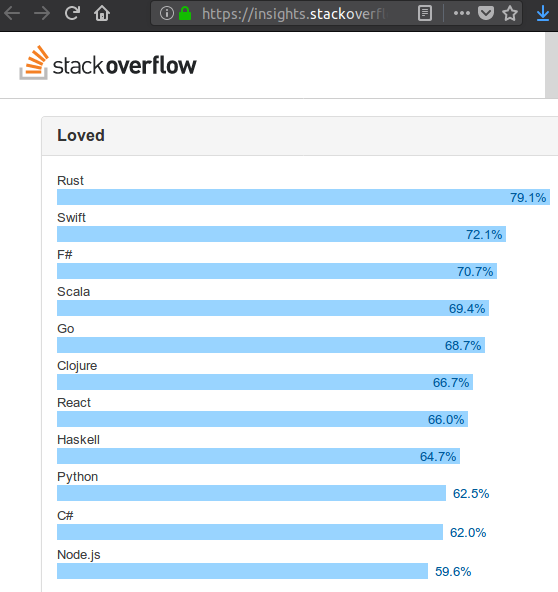
\includegraphics[width=0.9\textwidth]{../img/w14/most-loved-2016.png}
\end{Slide}

\begin{Slide}{Hur ser framtidens jobbmarknad för Scala ut?}\SlideFontTiny

\hspace{-2.5em}\begin{minipage}{1.0\textwidth}
Jobbmarknaden för Scala växer globalt och i Sverige:

\begin{minipage}{0.48\textwidth}
\href{www.indeed.com/joptrends/q-scala.html}{www.indeed.com/joptrends/q-scala.html}\\
\vspace{1em}
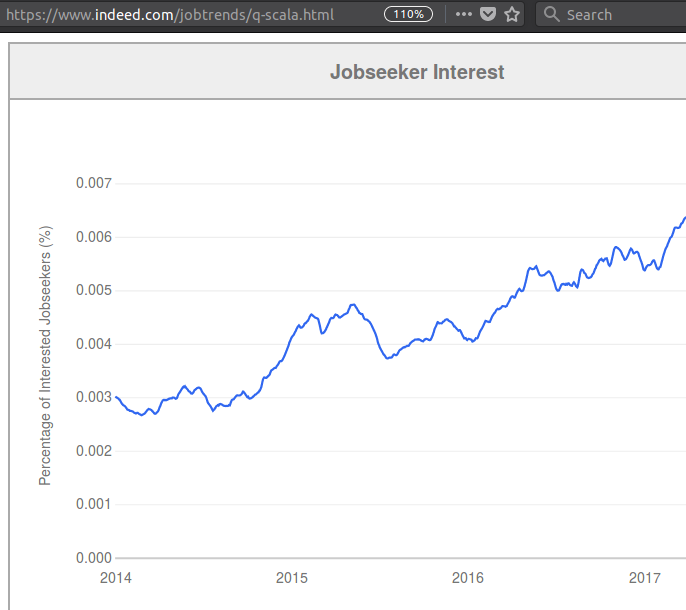
\includegraphics[width=1.0\textwidth]{../img/w14/scala-jobs-indeed-2017.png}~~
\end{minipage}
\hfill\begin{minipage}{0.48\textwidth}
\vspace{1.25em}
\href{https://www.linkedin.com/jobs/search/?keywords=scala&location=Sweden&locationId=se%3A0}{https://www.linkedin.com/jobs/search/?keywords=scala}\\
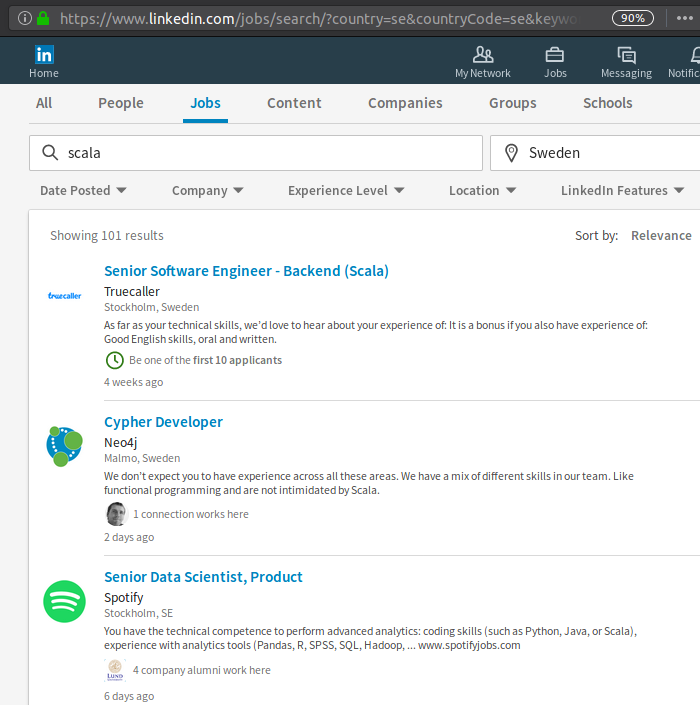
\includegraphics[width=1.2\textwidth]{../img/w14/scala-jobs-sweden-linkedin-2017-dec07.png}
\end{minipage}
\end{minipage}
\end{Slide}


\begin{Slide}{Hur ser framtiden ut för Scala?}\SlideFontSmall

Framtiden för \Emph{Scala}:
\begin{itemize}
\item Scala 2.12 bättre bytekod med lambda i JVM Java 8
\item Scala 2.13 bättre standardbibliotek
\item Ny kompilator: \Emph{dotty}; Nytt format ''över'' bytekod: \Emph{Tasty}
\item Scala.JS: dela kod+kompetens mellan backend och frontend
\item Scala native: kör Scala kompilerat direkt ''på metallen''
\item Scala-ramverk för stordata, massiv parallellism, AI, ...
\end{itemize}
\end{Slide}

\Subsection{Överraskning: LUFOSS}
\begin{Slide}{LUFOSS: Lund University Fund for Open Source Software}
\begin{itemize}
  \item Prisutdelning
  \begin{itemize}
    \item Studentpris
    \item Doktorandpris
    \item Hederspris
  \end{itemize}
  \item Gästföreläsning hederspristagare
\end{itemize}
\end{Slide}


\Subsection{Avslutning}

\begin{Slide}{Hoppas att pgk-kursen varit intressant och lärorik!}
\pause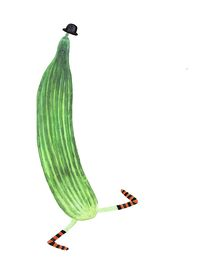
\includegraphics[width=5cm]{../img/gurka.jpg}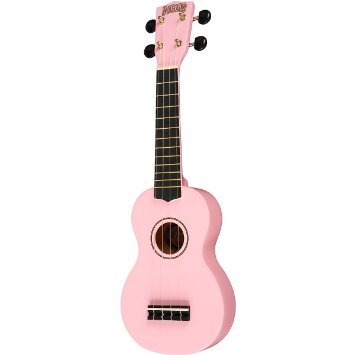
\includegraphics[width=5cm]{../img/ukulele.jpg}
\end{Slide}

\begin{Slide}{Ett stort TACK...}
\begin{itemize}
  \item
... till alla \Emph{handledare} som jobbat hårt för att ni ska lära er så mycket som möjligt!
\item ... till alla \Alert{studenter} som gått kursen för:
\begin{itemize}
\item ... att ni kämpat så hårt!
\item ... att ni ställt massor med frågor!
\item ... att det har varit så hög närvaro på föreläsningarna!
\item ... att ni hjälp till med värdefull återkoppling!
\item ... att ni är så konstruktiva och verkligen vill lära er!
\end{itemize}
\vspace{2em} \pause

\end{itemize}
\Alert{Ett stort LYCKA TILL på vägen till att bli en \\ kompetent och innovativ systemutvecklare!}
\end{Slide}



\fi


\end{document}
